\documentclass{article}

\usepackage{enumerate}
\usepackage[margin=1.5in]{geometry}
\usepackage{quiver}
\usepackage{tikzit}
\usepackage{tikz-cd}
\usepackage{amsthm}
\usepackage{amsmath}
\usepackage{amsfonts}
\usepackage{amssymb}
\usepackage{mathrsfs}  
\usepackage{braket}
\usepackage{mathtools}
\usepackage{lmodern}
\usepackage{float}
\usepackage{upgreek}



\newtheorem{theorem}{Theorem}[section]
\newtheorem{lemma}{Lemma}[section]
\newtheorem{corollary}{Corollary}[section]
\newtheorem{conjecture}{Conjecture}[section]
\newtheorem{proposition}{Proposition}[section]
\newtheorem{propositionph}{$\text{Proposition}^{ph}$}[section]

\theoremstyle{definition}
\newtheorem*{definition}{Definition}

\DeclareMathOperator{\wind}{wind}
\DeclareMathOperator{\Free}{Free}
\DeclareMathOperator{\Sym}{Sym}
\DeclareMathOperator{\Hom}{Hom}
\DeclareMathOperator{\swap}{swap}
\DeclareMathOperator{\id}{id}
\DeclareMathOperator{\SO}{SO}
\DeclareMathOperator{\SL}{SL}
\DeclareMathOperator{\GL}{GL}
\DeclareMathOperator{\End}{End}
\DeclareMathOperator{\ev}{ev}
\DeclareMathOperator{\coev}{coev}
\DeclareMathOperator{\op}{op}
\DeclareMathOperator{\tr}{tr}
\DeclareMathOperator{\FPdim}{FPdim}
\DeclareMathOperator{\Rep}{Rep}
\DeclareMathOperator{\Aut}{Aut}
\DeclareMathOperator{\MCG}{MCG}
\DeclareMathOperator{\func}{func}

\newcommand{\RR}{\mathbb{R}}
\newcommand{\ZZ}{\mathbb{Z}}
\newcommand{\QQ}{\mathbb{Q}}
\newcommand{\CC}{\mathbb{C}}

\newcommand{\NN}{\mathcal{N}}
\newcommand{\Cc}{\mathcal{C}}
\newcommand{\C}{\mathscr{C}}
\newcommand{\Dcat}{\mathscr{D}}
\newcommand{\LL}{\mathcal{L}}
\newcommand{\D}{\mathfrak{D}}
\newcommand{\Z}{\mathcal{Z}}
\newcommand{\OO}{\mathcal{O}}
\newcommand{\PP}{\mathcal{P}}

\newcommand{\0}{\left|0\right>}
\newcommand{\1}{\left|1\right>}


\renewcommand{\P}{\textsc{\textbf{P}}}
\newcommand{\BPP}{\textsc{\textbf{BPP}}}
\newcommand{\BQP}{\textsc{\textbf{BQP}}}
\newcommand{\NP}{\textsc{\textbf{P}}}
\newcommand{\NOT}{\textsc{NOT}}
\newcommand{\CNOT}{\textsc{CNOT}}
\newcommand{\AND}{\textsc{AND}}
\newcommand{\OR}{\textsc{OR}}

\newcommand{\one}{\mathbf{1}}
\renewcommand{\Set}{\mathbf{Set}}
\renewcommand{\Vec}{\mathbf{Vec}}

\newcommand{\dual}{\prescript{*}{}}



\graphicspath{ {./images/} }
\numberwithin{figure}{section}
\setcounter{section}{-1}



\title{The Algebraic Theory\\ of \\ Topological Quantum Information}
\author{by Milo Moses}

\date{\textit{California Institute of Technology} \\ [2ex] \today}


\begin{document}


\maketitle


\begin{abstract}
This book aims to give a comprehensive account of the algebraic theory of topological quantum information. It is intended to be accessible both to mathematicians unfamiliar with quantum mechanics and theoretical physicists unfamiliar with category theory. Additionally, this text should make a good reference for working researchers in the field. A primary focus of this text is balancing powerful algebraic generalities with concrete examples, principles, and applications.
\end{abstract}


\newpage

\tableofcontents

\newpage


\section{Preface}
\label{Preface}

This book is a mathematical treatment of topological quantum information, with a focus on formal algebraic aspects and a special eye towards topological quantum computation. This manuscript began as an extended set of notes from a course on topological quantum field theory given by Zhenghan Wang in the winter of 2022 at UC Santa Barbara. Through his courses, his private tutoring, and his reccomendations, Zhenghan took me from a state of almost complete ignorance of mathematical physics to being a young researcher in the field. I am greatly emdebted to him for this, and it is certain that this book would not have existed without his guidance - he richly deserves of my apple.

This book would not have been possible without the tutelage of my esteemed mentors. Those who most direct contributed are the ones who used their time and energy to teach me topological quantum information - Dave Aasen, Mike Freedman, and Yuri Lensky. There are also those who took a chance on a young mathematician when they had every reason not to - Roald Dejean, Peter Bloomsburgh, Edward Frenkel, and Ken Ribet.

[WORK: There's some other people to thank. Andrew Sylvester for letting me try out my arguments on him. ]

Great pains have been taken to make this book as pedagogical and accessable as possible. The hope is that it should be readable by both mathematicians unfamilar with quantum mechanics as well as theoretical physicists unfamiliar with category theory. A primary focus of this text is balancing powerful algebraic generalities with concrete examples, principles, and applications. The prerequisites for this book are a undergraduate-level understanding of topology, linear algebra, and group theory, as well as a popular-science level of familarity with quantum mechanics.

There are already many great references to learn aspects of the material covered in this book. An excellently written and relatively complete book on topological quantum information from the perspective of a physicist is Steven Simon's text \cite{simon2023topological}. Simon's book is algebraic, but does \textit{not} include any category theory. The main references for the relevant category theory are Bakalov-Kirillov \cite{bakalov2001lectures} and Etingof-Gelaki-Nikshych-Ostrik \cite{etingof2016tensor}. While both excellent texts, they suffer notable shortcomings for learning topological quantum information. Bakalov-Kirillov was written in 2001, making it outdated. Etingof-Gelaki-Nikshych-Ostrik is modern, but makes no connections to physics and does not use the language of string diagrams. The manuscript most similar to this one is Kong-Zhang's preprint \cite{kong2022invitation}. We distinguish ourself from Kong-Zhang by our different choice of topics, our different choice of treatment, and our extended scope. Other relevant books and review articles include Wang's monograph \cite{wang2010topological} and Kauffman-Lomonaco's quantum topology themed review \cite{kauffman2009topological}.

[WORK: I will add a section detailing the structure of this book, and how it should be read. I have not written enough for this to be useful yet.]

\section{Overview}
\label{overview}

\subsection{Conceptual introduction}
\label{conceptual introduction}

\subsubsection{Motivation and applications}

I will take as a definition \textit{topological quantum information} to be the study of information in topological quantum systems. A topological quantum system is some mathematical or physical system which is in a fundamental sense described by the mathematics of both quantum mechanics and topology. The term \textit{quantum system} here is used in contrast to \textit{classical system}. The flow of current through a conducting copper wire is described perfectly well by classical electromagnetism, whereas the flow of current through a superconducting niobium-titanium wire necessarily requires quantum mechanics for its description.

The term \textit{topological system} is used in contrast to \textit{geometric systems}, though the term “geometric system” is a nonstandard one. In a geometric system measurable quantities and phenomena depend on quantitative local aspects of the system - the distance between wires, the exact shape of some sample, or the curvature of some component. In a topological system measurable quantities and phenomena depend only on qualitative global aspects of the system - whether two wires cross or not, whether a sample is connected or not, whether a component curves into a ball or has a boundary.

I say that this book is about “topological quantum information” and not “topological quantum systems” for two reasons. The first is to highlight the fact that there is more to a topological quantum systems than its global topological properties. Topological quantum systems also have local geometric descriptions which are important for understanding many phenomina. However, we will mostly be ignoring these local effects in favor of focusing on global topological properties. The beauty of topological quantum systems lies exactly in the fact that this global perspective retains all the essential information in the system. The second reason is to highlight this book’s eye towards topological quantum computing, the idea of making computers using topological quantum systems. 

Since Peter Shor’s 1994 discovery of an efficient factoring algorithm on quantum computers \cite{shor1994algorithms}, the primary goal of quantum information theorists has been to harness quantum information sufficiently well so that it can be used to make an efficient scalable quantum computer. One of the major hurdles in achieving this goal is that quantum information is \textit{fragile}. Small amounts of noise coming from nearby electromagnetic fields or imperfections in experimental devices are often enough to affect the information being stored, resulting in \textit{errors} in the computation. In the early days of quantum computing it was not clear whether there was any way around this problem. Perhaps the inherent fragility of quantum information would make quantum computation impossible. This turned out to be false.

The beautiful observation is that errors are not nearly as catastrophic in \textit{topological} quantum systems. Errors are typically local. By definition the information topological systems does not depend on local properties, and hence is not affected by local changes. Hence, under suitable conditions, topological systems are naturally error resistant! In the same way that invariants of topological spaces are supposed to be invariant under deformations in pure mathematics, information in topological systems is invariant under errors in mathematical physics. Hence, to solve the problem of noise all one has to do is make a \textit{topological} quantum computer! This observation was made in 1997 and is due independently to Alexei Kitaev and Michael Freedman \cite{kitaev2003fault, freedman1998p}. Since then topological quantum computing has grown and evolved, finding its way into almost every modern proposal for fault-tolerant quantum computing.

The first approach to topological quantum computing is to use a physical material, some literal condensed collection of atoms, which naturally behaves as a topological quantum system. These exist and have been studied for a long time. For instance, a two dimensional sheet of graphene behaves topologically when it is subjected to low temperatures ($\approx$5 degrees Kelvin) and large magnetic fields ($\approx$15 Teslas) \cite{bolotin2009observation}. Topological quantum materials which can be used to make scalable quantum computers require intricate experiments to operate, which has been the most prominent roadblock in this approach.

The second approach to topological quantum computing is to artificially construct a topological system within a geometric one. The function of a quantum computer, almost by definition, is to simulate quantum systems. In particular, it can simulate \textit{topological} quantum systems. Since topological systems are resistant to local errors, this means that the original computer which is simulating the topological system will itself become resistant to local noise! This works exactly as described as long as the simulation itself is local, that is, local effects in the original system correspond to local effects in the simulated system. This technique of simulating topological systems to inherit their error-resistant properties is known as \textit{topological quantum error correction}. The advantage of this approach is that it works on any hardware available. The disadvantage is that to perform useful computations one must pass through simulation involved the topological quantum error correction. This additional layer adds a hefty amount of overhead, which can eat up the majority of runtime and resources. It is for this reason that \textit{efficient} topological quantum error correction is an important and active area of research.

\begin{figure}
\[\begin{tikzcd}
	& \begin{array}{c} \substack{\text{topological}\\ \text{quantum}\\\text{materials}} \end{array} \\
	\begin{array}{c} \substack{\text{topological} \\ \text{quantum} \\ \text{information}} \end{array} \\
	& \begin{array}{c} \substack{\text{topological}\\\text{quantum}\\ \text{error correction}} \end{array}
	\arrow["\begin{array}{c} \substack{\text{intrinsic}\\\text{realization}} \end{array}", from=2-1, to=1-2]
	\arrow["\begin{array}{c} \substack{\text{local}\\\text{simulation}} \end{array}"', from=2-1, to=3-2]
\end{tikzcd}\]
\caption{The two major branches of topological quantum information.}
\end{figure}

Of course, the above discussion presents only one motivation for topological quantum information and only one example of an application. Topological quantum materials open a whole world of potential applications, and it seems they may play an important role in the techonologies of the future \cite{ramirez2020dawn}. Some proposed applications include processing classical information using topological defects in magnetic devices (with the end goal of making high-speed low-energy transmissions) \cite{marrows2021perspective, vsmejkal2018topological}, creating highly sensitive photodetectors (with the end goal of making night-vision goggles or sensors) \cite{chan2017photocurrents}, creating technolgies with high thermoelectric effect (with the end goal of making efficient fridges or electric generators) \cite{skinner2018large}, creating highly-efficient transistors \cite{fuhrer2021proposal}, and engineering tiny electrical components \cite{viola2014hall, placke2017model}. 

This breadth of potential applications is due in part to the number of different types of topological materials which have been discovered or theorized. This includes quantized Hall states \cite{von202040}, topological insulators \cite{hasan2010colloquium}, fractional Chern insulators \cite{regnault2011fractional}, Weyl/Dirac semimetals \cite{armitage2018weyl}, and topological superconductors \cite{sato2017topological}. The contents of this book certainly do not provide the entire picture for any of these materials. However, the hope is that it gives a picture of the algebraic structures within them, hence helping readers think both concretely and conceptually about these materials and their applications.

\subsubsection{Mathematical picture}

The term \textit{topological quantum system} is broad. To get a rigorous mathematical subject, we will focus on a specific type of topological quantum system known as a \textit{topologically ordered} quantum system. Topological order is much more precise, though there are still conflicting definitions in the literature. Specifically, I will be focusing on \textit{(2+1)-dimensional} topological order. Here, I am using the physicist convention of using (2+1)D to refer to two space dimensions and one time dimension. That is, I will be discussing a locally flat topologically ordered system. For example, a single sheet of graphene at low temperatures and large magnetic fields can exhibit a form of (2+1)D topological order, and any quantum computer running topological quantum error correction can also exhibits a form of (2+1)D topological order.

\begin{center}
\fbox{All systems in this book are two-dimensional unless stated otherwise.}
\end{center}

Topological quantum systems can be described in many different ways. In this book we will take an \textit{algebraic} approach. [WORK: what does it mean to take an algebraic approach to something?]. The algebraic structure which houses the algebraic data of a (2+1)D topologically ordered system is known as a \textit{modular tensor category}. These algebraic structures are the main mathematical object of this text. Once one has a modular tensor category it is easy to manipulate the stored information to perform computations. This gives us the overall schema of our mathematical discussion, illustrated visually below:

\begin{equation*}
\tikzfig{mathematical-outline}
\end{equation*}

In Chapter [ref] we describe topological order. In Chapter [ref] we describe topological order algebraically in terms of modular tensor categories. In Chapter [ref] we describe further algebraic structures which lie beyond plain modular tensor categories, which allow us to describe more complex behaviors in topological order. Finally, in Chapter [ref] we will use the tools we have established to detail several algorithms and procedures for topological quantum computaiton. Two introductory chapters are also included: Chapter [ref] which establishes the theory of finite dimensional quantum systems and Chapter [ref] which establishes category theory.

\subsubsection{History of the subject}

Like with any sufficiently rich subject, the history of topological quantum information can be traced back as far as one wants. So let us do exactly that. The first use of topology in information science was roughly 2600 BCE, with the South American \textit{Quipu} \cite{ascher1981code}. Quipu are intricate knotted strings typically made out of cotton fibers. The knots in the string are used to store various types of information, typically numbers. Mathematically we say that Quipu store their information in knot invariants, and hence hold \textit{topological} information.

Quipu were so successful that they remained the primary method of information processing in much of South America for thousands of years. They reached their peak of usage in the 15th century via the Inca empire. The Inca empire was the largest pre-Columbian empire in the western hemisphere, with over ten million subjects and spanning over two million square kilometers. Despite their intricate government, the Incas had \textit{no written language}. This distinguished them from their contemporary empires, such as the Mali, Mongolian, or Chinese empires, which all relied on the written word. The success of the Inca empire can be seen as a testament to the versatility and power of knot invariants. The difference between the Inca and modern proposals for topological quantum computers is that instead of the strings being made out of cotton fibers they are made out of the spacetime trajectories of quasiparticles in topological systems.

Just like the history of topology in information science can be traced back to the origin of information science, the history of topology in quantum mechanics can be traced back to the origins of quantum mechanics. There is a 1931 paper of Paul Dirac \cite{dirac1931quantised} which introduces many of the ideas which would become foundational to topological quantum mechanics. In the 1950s, explicitly topological ideas such as the Aharanov-Bohm effect \cite{aharonov1959significance} and the theory of point defects by Tony Skyrme \cite{skyrme1962unified} were beginning to emerge. By the 1970s nontrivial abstract topological considerations were leading to novel contributions to contemporary physics, such as the theoretical description of the A-phase of superfluid Helium-3 \cite{anderson1977phase} and the theory of phase transitions in the xy model proposed by Kosterlitz-Thouless \cite{kosterlitz1973ordering}. These results were associated with the 1996 and 2016 Nobel prize respectively.

It was in the 1980s, however, that topology established itself as one of the leading themes in condensed matter physics. The discovery of the quantum Hall effect in 1980 \cite{klitzing1980new} and the subsequent discovery of the fractional quantum Hall effect in 1982 \cite{tsui1982two} gave the first examples of topologically ordered systems in our modern sense of the word, and resulted in the 1985 and 1998 Nobel prizes respectively. These systems gave theorists the license to dream big about what possibilities could lie ahead. This led to major work by theorists such as Frank Wilczek \cite{wilczek1982quantum, arovas1985statistical}, Duncan Haldane \cite{haldane1983nonlinear, haldane1988model}, and others on the theory of topological quantum systems.

The most notable of these theorists for our present story is Edward Witten, with his introduction of \textit{topological quantum field theory} in 1988 \cite{witten1988topological}. This work not only put the modern experiments within a larger context, but it also connected these developments to a parallel story which had been developing within pure mathematics. Namely, knot theory. In 1984 Vaughn Jones discovered his landmark knot invariant, which was powerful in its ability to distinguish between non-equivalent knots \cite{jones1997polynomial}. This marked the first major progress in the field since Alexander's invariant in 1928 \cite{alexander1928topological}. However, Jones’ construction was steeped in opaque subfactor theory, so much so that the fact that it resulted in knot invariant felt almost like a happy accident. Hence, a widespread topic on the mind of contemporary mathematicians was how to properly interpret the Jones invariant, and how to construct other invariants like it. Witten seemed to answer both. After defining topological quantum field theory, he showed how the Jones invariant could be obtained as an observable quantity within a certain field theory \cite{witten1989quantum}! This shocking result gave a new interpretation of the Jones invariant in terms of mathematical physics which was appealing to experts. Seeing as the Jones invariant was constructed from a topological quantum field theory, it was natural to expect that other field theories might give new invariants which could distinguish between even more knots. This vision of invariants in low-dimensional topology constructed using topological quantum field theory became known as \textit{quantum topology}, and evolved into its own discipline in the following years.

This brings us to 1997. Quantum topology is an active area in pure mathematics, and topological themes in condensed matter physics are at the forefront of the field. The open problem is how to construct a fault tolerant quantum computer. Peter Shor had recently discovered his factoring algorithm \cite{shor1994algorithms}, and there was debate about whether scalable quantum error correction was possible \cite{landauer1995quantum}. This led to two independent proposals for topological quantum computation in the same year. One was by the mathematician Michael Freedman \cite{freedman1998p}. His vision was clear. A recent paper had shown that computing the Jones invariant of knots was in general an NP-hard problem \cite{jaeger1990computational}. However, by the work of Witten, the Jones invariants of knots were observables in certain topological quantum field theories. Hence, if one could construct physically a topologically ordered system which was described by Witten’s topological quantum field theory then the Jones polynomial of knots could be computed efficiently by making measurements on the system. Hence, one would obtain a very powerful computer! This was Freedman’s proposal.

The other proposal was made by theoretical physicist Alexei Kitaev \cite{kitaev2003fault}. His proposal was much more precise. He gave a toy model for a certain family of topologically ordered systems. He then outlined a technique for storing and manipulating information within these systems. The deep observation was that these systems were intricate enough that they could be used to make a powerful quantum computer \cite{mochon2003anyons}.

In the subsequent years Freedman and Kitaev teamed up with collaborators Zhenghan Wang, Michael Larsen, and others to study the new field of topological quantum information and the possibility of constructing a topological quantum computer. One of the first major results was that no topological quantum computer could be more powerful than a standard quantum computer \cite{freedman2002simulation}. This went against Freedman’s original hope to solve NP-hard problems using topological quantum computers. Freedman’s mistake was in asserting that topological quantum computers could compute the Jones polynomial. The measurements which give the Jones invariant in topological quantum field theory will always be \textit{approximate}. Approximating the Jones invariant in this way is computationally easier than evaluating the Jones invariant exactly. In fact, this way of approximating the Jones invariant is \textit{not} NP-hard - it can only be used to solve problems which could efficiently be solved using standard quantum computers.

The second major result of Freedman, Kitaev, Wang, and Larsen was the converse of their first result \cite{freedman2002modular}. Namely, they showed that every quantum algorithm can be efficiently run on a topological quantum computer. They do this by showing that every quantum algorithm can be efficiently reinterpreted in terms of computing the Jones invariant of some knot. In this way computing the Jones invariant is not NP-hard, but it is a \textit{universal problem} for quantum computation. They then formalize Freedman’s ideas about topological quantum field theory, and show directly that realistic operations on a topologically ordered quantum system described by Witten’s quantum field theory can be used to compute the Jones invariants of knots.

Together, these two results show in a real sense that topological quantum computing is equally powerful as standard quantum computing with quantum circuits. This laid the groundwork for fruitful studies of fault-tolerant topological quantum computing, both using error correcting codes and physical materials. This has resulted in a great number of important results, which we will discuss at length throughout the rest of this manuscript.

\subsection{Technical introduction}
\label{technical introduction}

\subsubsection{Principles of topological quantum information}

In this section we will lay out the general principles of topological quantum information. As an organizational tool, these principles are introduced one by one as we construct a sample topological system. This example is meant to be representative of the systems we will encounter throughout this text, and within the broader field of topological quantum information. As a further organization tool, this example is constructed with the stated goal of obtaining a topological quantum computer.

Our system will be flat, containing only two spatial dimensions. Our system will be mostly homogenous, essentially identical everywhere, at the exception of finitely many localized regions. These regions will differ substantially from the top-dimensional homogeneous bulk. These localized regions are called \textit{quasiparticles}. The beauty of systems like these is that they behave as though the homogeneous bulk were empty, and the quasiparticles were fundamental particles within the bulk. In fact, in its algebraic description, these topological systems are \textit{identical} to ones in which the homogenous bulk is empty and the quasiparticles are fundamental particles. This is where the term quasiparticle arises. It is important however to remember that in most relevant applications the bulk is \textit{not} empty and the quasiparticles are \textit{not} fundamental particles. The bulk is typically some highly entangled quantum wavefunction, and the quasiparticles are emergent phenomena made up of smaller microscopic degrees of freedom.

\begin{figure}[h]
\begin{center}
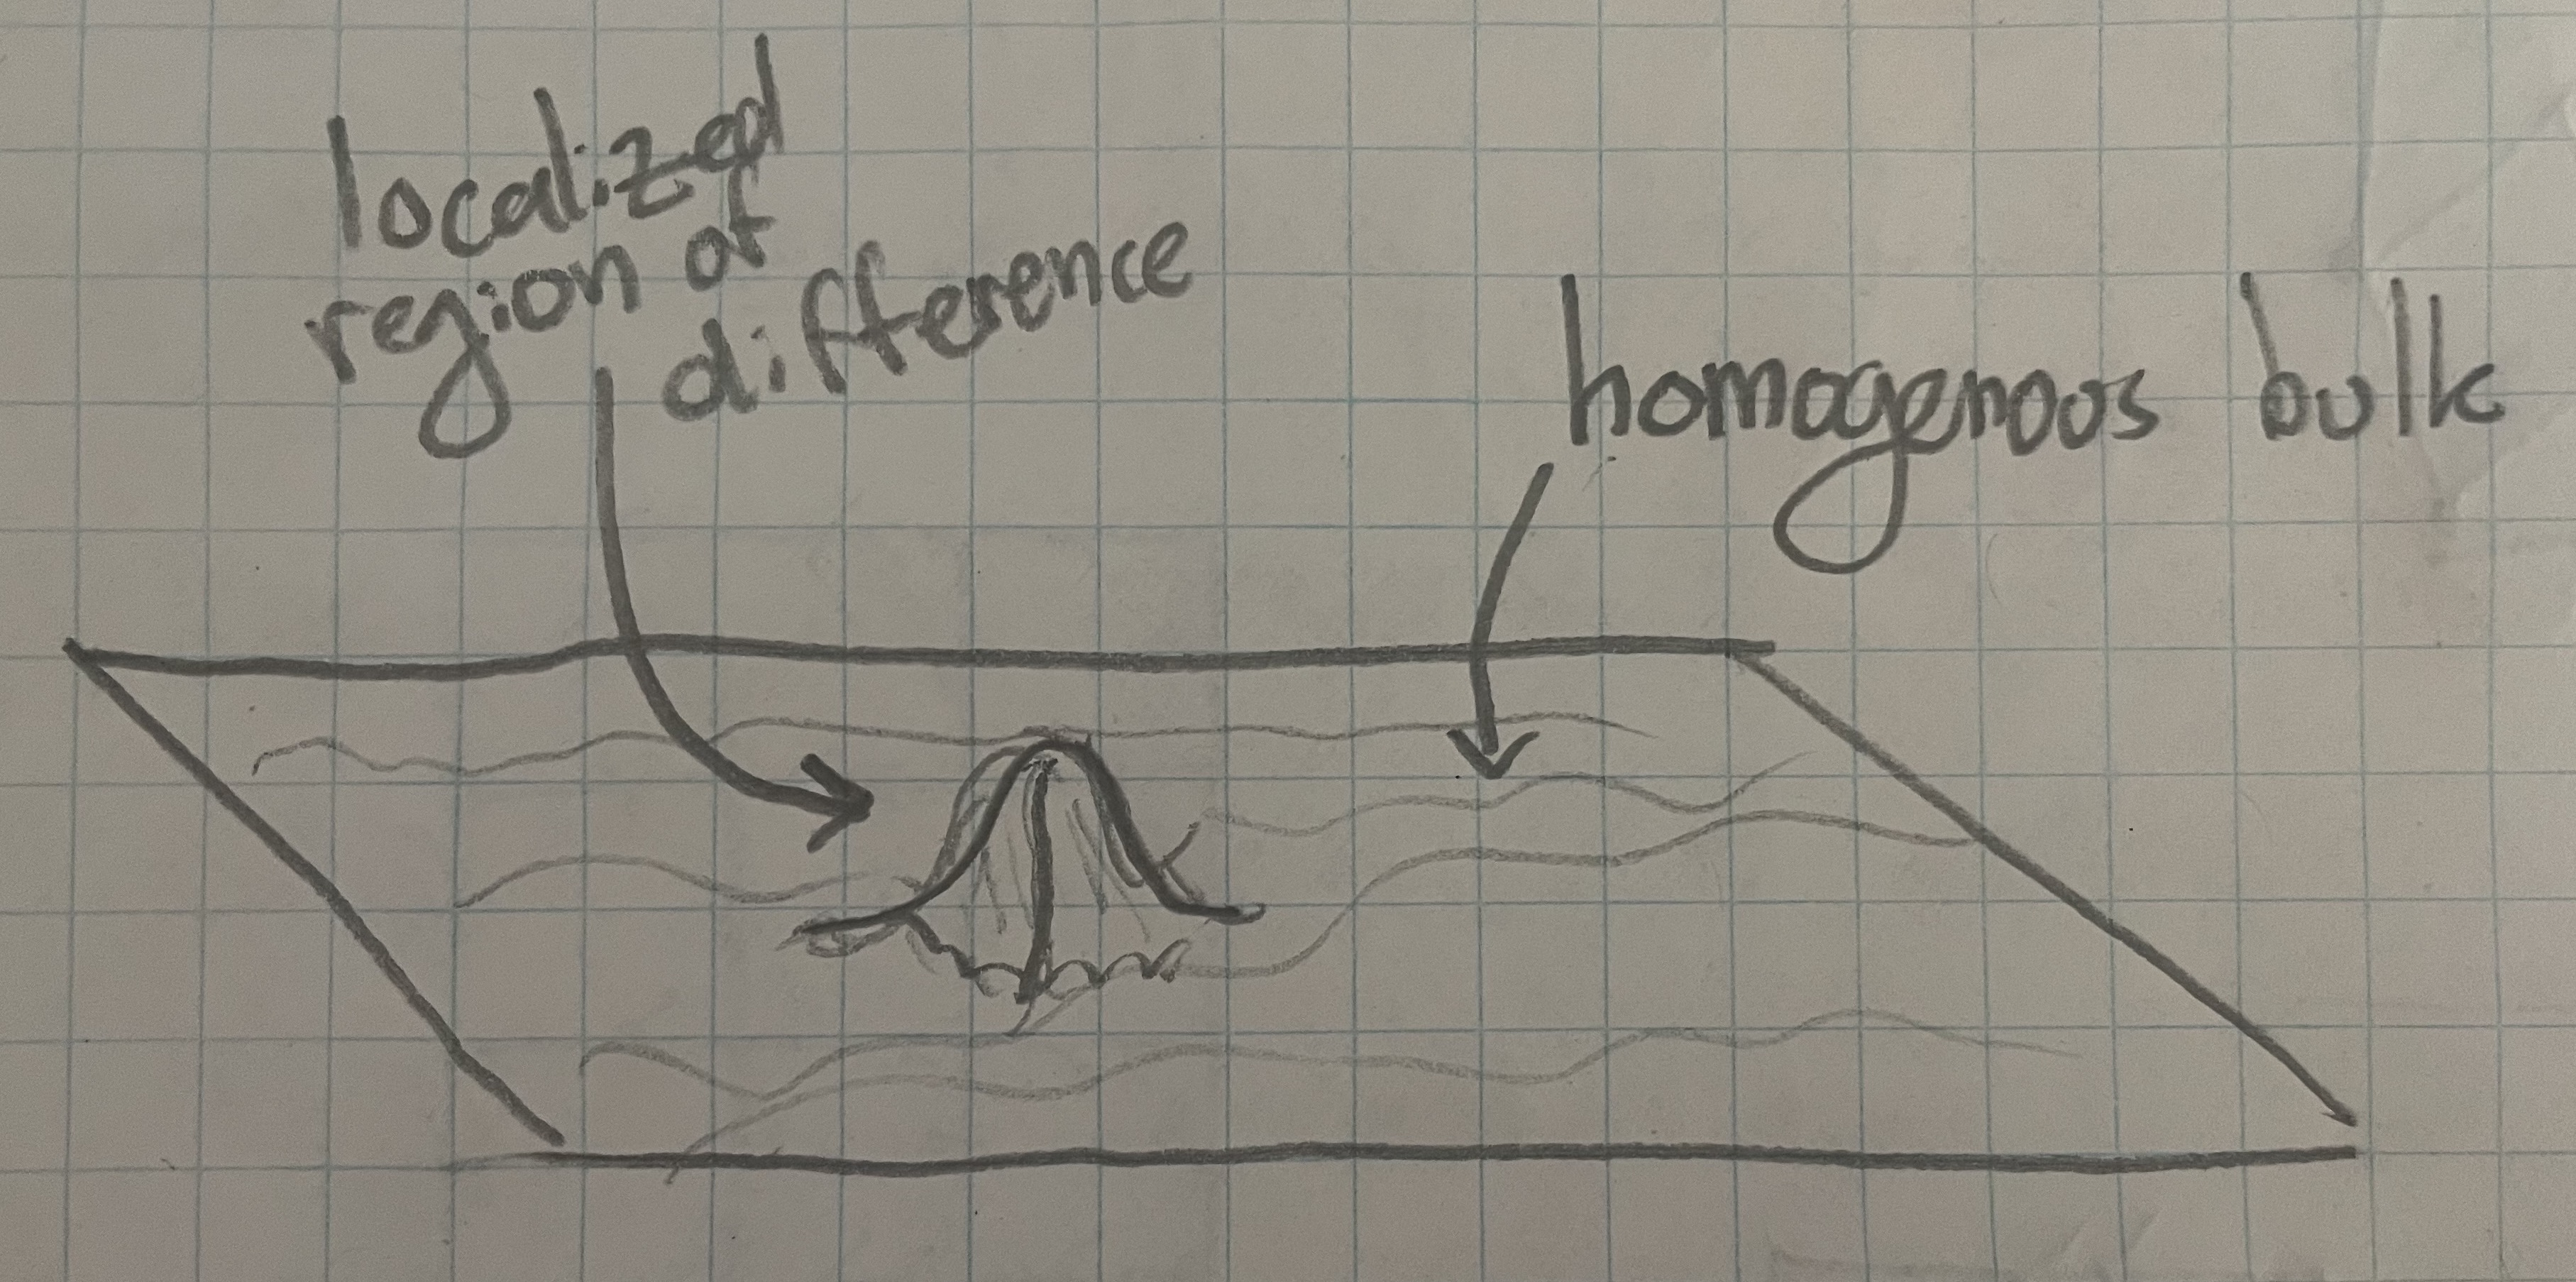
\includegraphics[scale=.04]{quasiparticle}
\end{center}
\caption{A quasiparticle in a two dimensional system}
\end{figure}

Our aim is to build a computer. In general this requires three components:

\begin{enumerate}
\item A method of storing information;
\item A method of manipulating information;
\item A method of reading out information.
\end{enumerate}

Information is stored in the state of the system - the bulk is described by some parameters, and the details of those parameters encodes information. Our method for manipulating information is \textit{braiding}. Braiding is the process whereby quasiparticles are moved along continuous paths around one another. There are two important points about braiding to keep in mind. The first is that braiding changes the state of the system. Even though the quasiparticles might be in identical places before and after the braid, the details of the system will change - there is more to the state of the system than just the positions of the quasiparticles. The second point is that the way that the state of the system changes depends \textit{only depends on the topology of the braid}, and not the geometry. Small deformations in the path taken by the quasiparticles do not affect the result - only global changes, like whether a path is taken clockwise or counterclockwise, makes a difference. This invariance is due to the fact that our system is topological. In geometric systems we expect the exact path taken by quasiparticles matters a great deal. The independence of the details of the paths is extremely specific to topological systems, and in the present setting is the \textit{defining topological feature}.

[WORK: add braid diagrams to demonstrate what braiding is like. Doesn't have to be string-diagram like - probably best to keep it in-plane 2D.]

At this point we can already see we have succeeded in our goal of making our computations fault-tolerant. Noise in the system will correspond to uncontrolled perturbations in the trajectories of the quasiparticles. This uncontrolled movement won’t change global properties of paths taken, and hence will not change the action of the braids on the system. That is, small errors won't affect computation! Of course, large enough errors could unintentionally make one quasiparticle wind around another. This would change the topology of the braid and hence ruin the computation. These errors are controllable, however, by moving the quasiparticles far apart and limiting the magnitude of the noise.

The final step in making our computer is to introduce a method for reading out information. This is done using \textit{fusion}. Fusion is the process whereby two quasiparticles are brought together, resulting in a single quasiparticle. In sufficiently complicated topological systems the result of fusion depends on the details of the state of the overall system. That is, the result of fusion can be used as a way of reading out information about the state! In its most basic form, when two quasiparticles fuse they can either result in a localized region which is identical to the homogenous bulk or is different from the homogenous bulk. If they result in a localized region identical to the bulk we say that the two quasiparticles have \textit{annihilated} each other. This can be seen as the difference between constructive and destructive interference. Two waves can either have destructive interference and annihilate each other when they meet, or they can have constructive inteference and result in a new wave. Measuring whether or not two quasiparticles annihilate upon fusion gives a method for reading out information.

In some situations, the result of fusion can even be nondeterministic. In this case the fusion can be repeated multiple times, which allows one to measure the \textit{probability} that two quasiparticles will annihilate each other. These probabilities are a rich source of data, and will serve as our way of reading out information in the current setting. The fact that our system is topological implies that the result of fusion does not depend on the specifics of the path taken, and hence this method of readout preserves the invariance of our computation to noise. This gives us a full picture of topological quantum computation, as seen in figure \ref{fig:TQC-outline}.

\begin{figure}
\begin{center}
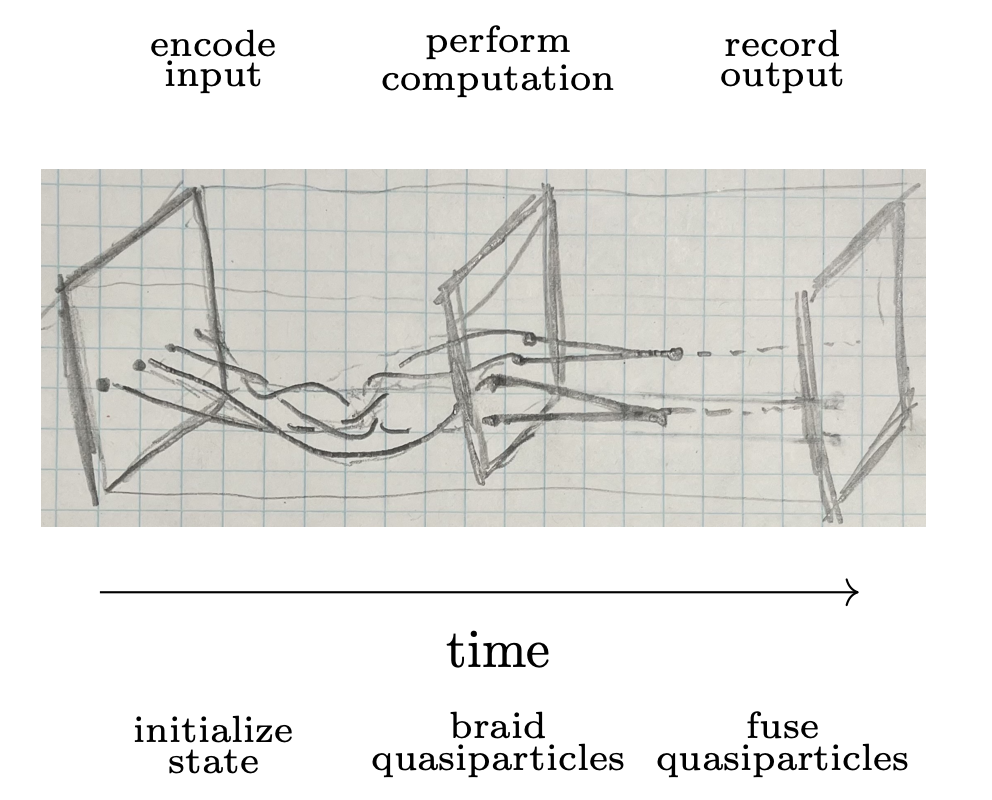
\includegraphics[scale=0.35]{TQC-outline}
\caption{A schematic of topological quantum computing}
\label{fig:TQC-outline}
\end{center}
\end{figure}

To make the above discussion more concrete, we will give a worked example. In this example we use a specific topological order known as the \textit{Fibonacci particle theory} to run Shor’s efficient quantum factorization algorithm \cite{shor1994algorithms}. The input of Shor’s algorithm is a positive integer. The output of Shor’s algorithm is the factorization of that integer. Shor’s algorithm is \textit{efficient} in the sense that it uses polynomially many quantum logic gates to arrive at its answer relative to the size of the input. Throughout this passage we will use \textit{efficient} and \textit{polynomially sized} interchangeably. The Fibonacci particle theory is a specific topological order, which describes in an algebraic fashion how the overall state changes when quasiparticles are braided and fused.

The first step in running Shor’s algorithm on a Fibonacci quantum computer is to translate the positive integer input into a certain braid. This is done using an efficient classical algorithm. The second step is to run this braid on a Fibonacci quantum computer. This is done by initializing some prescribed state and then braiding its quasiparticles. This initialization and braiding is performed repeatedly, and after every time two of the quasiparticles are fused. This lets us record a real number between 0 and 1, which is the probability that the two quasiparticles annihilate after the braiding. An efficient classical algorithm is then used to take this real number and obtain from it the factorization of the original input. Since all of these steps are efficient, it gives a topological quantum algorithm for factoring integers. The schematic for this process is shown below:

\begin{equation*}
\tikzfig{shor-fibonacci}
\end{equation*}

The magic in the above procedure is the existence of these two efficient classical algorithms: a first one for encoding integers into braids and a second one for decoding real numbers into factorizations. These algorithms are nontrivial. They are due to Freedman-Larsen-Kitaev-Wang \cite{freedman2002modular}. In fact, Freedman-Larsen-Kitaev-Wang showed that any problem which can be efficiently solved using a quantum circuit can also be solved using the Fibonacci particle theory, via a similar method of efficient classical preprocessing and postprocessing. It is in this sense that the Fibonacci theory is \textit{universal} for quantum computation.

The final step of this process would be to create a physical topological system which is described by the Fibonacci theory, which would serve as our quantum computer. In the realm of materials, the most promising approach seems to be to use specially tuned versions of the fractional quantum Hall system \cite{zhu2015fractional}. While these materials are theorized to host quasiparticles described by the Fibonacci theory, the difficulty of the experiment makes them inaccessible to current technology. There has been progress made on topological quantum error correcting codes which work by simulating the Fibonacci theory \cite{schotte2022quantum, schotte2022fault, xu2024non}. However these codes at the current moment have structural issues and require an unbearable amount of overhead to run, making them unfeasible to use on modern computers.

Progress on topological quantum computing has thus been focused on realizing topological particle theories other than the Fibonacci theory. These other theories can be constructed in more workable materials, and can be simulated as topological quantum error correcting codes with less overhead. The drawback of these other theories is that they are typically less computationally powerful, meaning that they require more tricks and techniques to achieve universal quantum computing. There are a great number of different proposals for how to achieve universal topological quantum computing, based on different particle theories, different methods of encoding information, different methods of manipulating information, and different methods of reading out information. It is an exciting time to be a theorist in the field of topological quantum information!

\subsubsection{Defects in ordered media}

We will now work through a complete mathematical example of a family of topological systems. Seeing as we don't assume that the reader is familiar with quantum mechanics, our examples will be \textit{classical} topological systems. Many of the important subtlties of topological quantum information are already present in the classical case. However, topological classical information is a smaller domain than topological quantum information - the reader should have a relatively complete grasp of the subject by the end of the chapter. Much of the discussion in this chapter is taken from an excellent review article by Mermin \cite{mermin1979topological}.

The family of systems we will describe goes by many names. In communities of experimentally focused physicists it goes by the name \textit{ordered media}. In mathematical physics communities it goes by the name \textit{classical field theory}. In pure mathematics it would be described as \textit{homotopy theory}. We will construct a system based on every topological space $M$. We will call $M$ the order space of our theory. We will assume throughout this chapter that $M$ is path connected.

To describe a system in physics, the first step is to define the space of possible states of the system. In this case, states will correspond to \textit{continuous maps $\phi: \RR^2\to M$}. We now give physical intuition for this choice of state space. The choice of $\RR^2$ as a source represents the underlying material. We are working on an infinite flat plane. Describing a function $\phi: \RR^2\to M$ amounts to choosing a value $\phi(x)$ for every point $x\in \RR^2$. In this way we imagine our system as being made up of infinitely many objects, one placed at each point in $\RR^2$, each of which has an internal state space $M$. Choosing the state of the overall system amounts to choosing the state of each individual object, that is, a value in $M$ for every point in the plane. The fact that $\phi$ must be continuous is a compatibility condition between the states of the objects at nearby points. It says that nearby objects must have similar states. We now list some examples which are described by this model:

\begin{itemize}
\item \textbf{Classical xy model of a 2D electron gas}. This model describes a possible behavior electrons in a flat 2D plane. An electron can be modeled as a point particle with a magnetic dipole pointing in some direction. This magnetic dipole is known as the \textit{spin} of the election, and can point in any direction in the plane. The topological space of all possible directions in the plane is a circle. Hence, in this system, the order space $M$ is the circle. The fact that nearby electrons must have similar spins is known as Hund’s rule, and is the most fundamental incarnation of ferromagnetism. It is physically derived as a consequence of the Pauli exclusion principle.

\item \textbf{Superfluid Helium-3} One famous example of ordered media is superfluid helium-3. Helium is an element. It has two stable isotopes: helium-3 and helium-4. The vast majority of helium on earth is helium-4, but there still is naturally occuring helium-3. At extremely cold temperatures helium-3 undergoes a phase transition, and becomes a superfluid. There are several different superfluid phases helium-3 can go into: B-phase, dipole-locked A-phase, dipole-free A-phase. For our purposes we will work with the dipole-locked A-phase. Its order space is $M=\SO(3)$, the group of rotations in three dimensional space.

\item \textbf{Biaxial nematics}. The objects at every point in the biaxial nematic should be thought of as small rectangles with unequal side lengths. These rectangles can be oriented in any direction in three dimensional space. In practice these objects will often be molecular compounds. They will not be exactly rectangular, but have the same symmetry group as a rectangle which is enough for the model to be accurate. To compute the space of possible orientations of a small rectangle, we work by the method of symmetries. Choosing some reference orientation to start with, every rotation in three dimensional space brings the rectangles to new orientations. The space of orientations of the rectangle is hence equal to $\SO(3)$ modulo the rotations which fix the rectangle. That is, $M$ is equal to $\SO(3)$ modulo the symmetry group of a rectangle.
\end{itemize}

[WORK: add diagrams for all three models]

We will now analyze these systems. In doing this analysis we will want to use the ideas of \textit{deformation} and \textit{topological equivalence}. Of course, these ideas are vague and require rigorous notions to make precise. We define these notions now. [WORK: this need to be reworded, with a proper caveat about rigor. Maybe bring up Jordan curve theorem for a laugh. Need to figure out what the policy on statements is.]

We now add a picture of \textit{dynamics} into our model - how it will be changing through time. In particular, we image that as time passes the system changes continuously. Let $\phi_t:\RR^2\to M$ be the state of the system at time $t$. We image that if $t_0$, $t_1$ are similar times then $\phi_{t_0}(x)$ and $\phi_{t_1}(x)$ will be close. Formally, this means that the maps $\RR_{\geq 0}to M$ assigning $t$ to $\phi_t(x)$ is continuous for all $x\in \RR^2$. This captures our intuitive notion of \textit{deformation}. We will image that the state of the system is constantly changing by deformations.

The first thing to notice about our system is that it is not storing any topologically-invariant information. In particular, every state can be continuously deformed to every other state. This is a general fact from topology: every pair of maps $\phi_0,\phi_1: \RR^2\to M$ can be continuously deformed from one to the other.

Clearly, this means that our system is not complicated enough to build a computer yet because it cannot store information. We rectify the situation by introducing quasiparticles. These quasiparticles go by many names. In the theory of ordered media they are known as defects. In field theory they are known as particles. In homotopy theory they are known as point singularities. For the sake of brevity, we will use the term defect.

A defect is a point at which we will drop our condition that the state $\phi:\RR^2\to M$ be continuous. This is done by making $\phi$ \textit{undefined} at certain points. Our new system is called \textit{ordered media with finitely many defects}. The state space consists of pairs $(S,\phi)$, where $S\subset \RR^2$ is a finite set and $\phi: \RR^2\\ S\to M$ is a continuous map.

[WORK: add picture of defects in ordered media]

Dynamics in our new system still correspond to continuous deformations. The subtelty now is that the defects can move as the state is deformed. We call these \textit{defect-mobile deformations}.

The vision for building our computer is that the experimenter should have control of the trajectories of the defects. This means that the system will trasform under defect-mobile deformations with definite paths chosen by the epxerimenter, but the details of the rest of the deformation is arbitarily and uncontrollable.

We can now outline the big idea of how the computer will work. We will arrange $n$ defects on a line in the plane. We keep these defects still, so that the system is changing only by deformations which keep the defects in place. We call these \textit{defect-fixed deformations}. We store our information in the possible configurations of this system:

[WORK: information storage space = (states with n defects arranged in a line)/ (defect-fixed deformation)]

The way we act on this information is by moving the defects around each other. This movement of defects induces some defect-mobile deformation. The space we are storing our information in is invariant under defect-fixed deformation, but not defect-mobile deformations. Hence, moving the defects around non-trivial paths will have non-trivial action on the stored information. This action on stored information is exaclty how we perform our computations.

Finally, we must introduce a method for reading out information. This is done via fusion. Two defects can be brought together and fused. The result of this fusion is a topologically invariant quantity, and we will assume that it can be measured by an experimenter. In its most simple form, this amounts to detecting whether two defects annhilated or not.  This gives us some information about the state, which is the output of our computation.

[WORK: add schematic for this process]

In the rest of this chapter we will describe exactly what the space we are storing our information in looks like, how braids act on that information, and how this can be used to make a functioning computer. This will give a detailed picture of how topological computation works.

\subsubsection{The fundamental group}

To understand topological computation in ordered media we will need to put in some real work in analysing the system, and make some non-trivial observations. The structure of this analysis will be largely the same as the analysis which will be taking place throughout the rest of this book. We recall the overall outline of this text, which goes as follows:

[WORK: add outline.]

In this section we will do a very similar thing. We will take our physical model, ordered media, and take its algebraic description. That algebraic description can then be used for making a computer. Luckily for us, the algebraic theory underlying ordered media is much simpler than the algebraic theory underlying topological order: it's group theory. In particular, we will even assume that all relevant groups are \textit{finite}. In this way, modular tensor categories can be seen as vast quantum generalizations of finite groups. The schematic in our case is shown below:

[WORK: add outline w/ group theory instead of MTC.]

The way we go from defects in ordered media to group theory is by using a construction known as the \textit{fundamental group} from homotopy theory.

The fundamental group is derived from a careful analysis of loops in topological spaces. We first clairfy what we mean by \textit{loop}. Loops, for our purposes, are always \textit{oriented} and are allowed arbitrary self intersections. Examples of loops around a point are shown below:

[WORK: add pictures of loops.]

Formally, we define a loop in a topological space $M$ to be a continuous map $\alpha:[0,1]\to M$ such that $\phi(0)=\phi(1)$. Our main goal us to understand topological information. Topological information is stored in properties which are invariant under deformations. Hence, we are naturally interested in the space of loops up to deformation.

In the plane $\RR^2$ with a point removed, points up to deformation are classified by their \textit{winding number}. This winding number is an integer which says how many times the loop went around the point. This windingn number is an integer in $\ZZ$, with positive numbers corresponding to counterclockwise rotations and negative numbers corresponding to clockwise rotations. The loops in figure [ref] have their winding numbers given as an illustration of the concept.

The key ingredient we are missing is the \textit{group structure}. We want to get groups out of topological spaces, but so far all we have is a set. The group structure comes from composition. Given two loops we can compose them by first following one loop and then following the othe. In this language, we see the topologists' winding-number version of $1+1=2$ below:

[WORK: add 1+1=2 with winding numbers.]

This definition has a big problem though. To compose, we need to choice a point to start and stop two two loops being composed at. This special starting/stopping point is known as a \textit{basepoint}. This deal of choosing basepoints is very important for the theory. Formally, a loop in $M$ based at $m\in M$ is a map $\alpha:[0,1]\to M$ such that $\phi(0)=\phi(1)=m$. We define the composition of two loops $\alpha_0,\alpha_1$ in $M$ based at $m\in M$ to be

$$
(\alpha_1 \circ \alpha_0)(t)=
\begin{cases}
\alpha_0(2t) & 0\leq t \leq 1/2 \\
\alpha_1(2(t-1/2)) & 1/2 < t \leq 1.
\end{cases}$$

The reason we need to add the factors of $2$ is to ensure that the domain of the loop is still the unit interval $[0,1]$. Intuitively, to fit two loops in the same amount of time we had to speed-up both loops by a factor of 2.

We are now almost ready to define the fundamental group: we have defined based loops, and we have defined a rule for their composition. The last subtelty is in discussing what it means to deform based loops. In particular, should deformations be allowed to move the basepoint? The issue that we want to be able to compose our loops. To compose loops they need to have the same basepoint. If the basepoint moves then we will lose out composition structure. Hence, for the time being, we should only work with deformations which preserve the basepoint. With this subtelty out of the way, we can finally define the fundamental group. Given any connected topological space $M$ and any point $m\in M$, we define the \textit{fundamental group of $M$ based at $m$} to be the group

$$\pi_1(M,m)\coloneqq \left(\text{loops in $M$ based at $m$}\right)/\left(\text{basepoint preserving deformations}\right)$$

whose group structure is given by the composition of based loops. As an example, our earlier comments about loops around points can be summarized as the statement that $\pi_1(\RR^2\backslash\{p\},b)\cong \ZZ$ for any distinct points $b,p\in \RR^2$. The identity element in the fundamental group is the trivial loop which stays at its basepoint and doesn't move (formally, the constant map $\alpha:[0,1]\to M$), and inverses are given by reversing orientation (formally, the inverse of $\alpha:[0,1]\to M$ is $\alpha^{-1}(t)=\alpha(1-t)$.)

We can now start to use the fundamental group to analyse defects in ordered media. The first major insight is that loops in physical space yield loops in order space. Let $S$ be a finite set of defects and let $\phi: \RR^2 \backslash S \to M$ be a state. Given any loop $\alpha$ in $\RR^2\backslash S$ based at $b\not\in S$, postcomposing with $\phi$ gives a loop in $M$:

$$(\phi \circ \alpha): [0,1]\xrightarrow{\alpha} \RR^2 \backslash S \xrightarrow{\phi} M.$$

This loop has basepoint $(\phi \circ \alpha)(0)=(\phi\circ \alpha)(1)=\phi(b)$. This gives an element of $\pi_1(M,\phi(b))$. Given any state $\phi$ and given any loop $\alpha$ based at $b$, we call the corresponding element of $\pi_1(M,\phi(b))$ the \textit{winding number of $\phi$ along $\alpha$}. This sort of winding number generalizes the standard notion of a winding number of a loop around a point discussed before.

Now, consider the system with $n$ defects arranged in a line. We can choose a basepoint $b$ above all of the defects. We add loops $\alpha_i$ based at $b$ for each $1\leq i \leq n$, each of which go directly around defect $i$ counterclockwise exactly once. This is depicted visually below:

[WORK: add picture.]

Given any ordered state $\phi$ on this system, we can take the winding numbers of each loop $\{\alpha_i\}_{i=1}^n$. These winding numbers all live in $\pi_1(M,\phi(b))$. Hence, to each state we can assign an element in the $n$-fold Cartesian product $\pi_1(M,\phi(b))^n$.

Fantastically, the values in $\pi_1(M,\phi(b))^n$ change in a well-behaved way under braids. We use a $2$-defect system to illustrate the principle.

[WORK: add good pictures to show why making $g_1$ go under $g_2$ maps $(g_1,g_2)$ to $(g_2,g_1)$. Talk a bit about it in words too]

This gives us a picture for how our computer works: information is stored in the winding numbers of the defects, and braiding acts by conjugating the winding numbers by each other.

There are a still a few lingering points that need to be sorted out before we can start building our computer. The first is the issue of whether our information being stored is actually invariant under defect-fixed deformations. Unfortunately, it is \textit{not}. The problem is that deformations in general have no reason to preserve the value of $\phi(b)$. The deformations will hence change the basepoints. However, elements of the fundamental group are only defined up to basepoint-preserving deformations! Hence, deformations of the state will change its winding numbers. In general we have the following key relation:

$$\left(\text{loops in $M$ based at $m$}\right)/\left(\text{basepoint preserving deformations}\right)= \pi_1(M,m)$$

$$\left(\text{loops in $M$ based at $m$}\right)/\left(\text{arbitrary deformations}\right)= \left(\text{conjugacy classes in }\pi_1(M,m)\right).$$

The intution for this above fact is as follows. Let $\alpha$ be a loop based at $b$. Let $\alpha'$ be the same loop but with a different choice of basepoint $b'$. Let $\epsilon$ be the portion of the loop between $b$ and $b'$. Going along $\alpha$ is the same as first going along $\epsilon$ to get to $b'$, then going along $\alpha'$, and then going along $\epsilon^{-1}$ to get back to $b$. Hence, we have $\alpha = \epsilon^{-1}\circ \alpha' \circ \epsilon$. Hence, choosing different basepoints amounts to conjugation. This is illustrated below:

[WORK: add diagram]

All this is to say that the winding numebrs in an $n$-defect ordered media state $\phi$ are not preserved up to defect-fixed deformations. Properly dealing deformations requires properly keeping track of conjugacy classes versus group elements. This sort of effort, however, is unnececary because it does not change any of the key takeways or any of the important concepts. Hence, \textit{we will assume that all of our deformations do not change the value of $\phi(b)$}. We will choose some element $m\in M$ and assume $\phi(b)=m$ is fixed. For physical motivation, one can imagine moving the basepoint far away towards infinity. Since all of our physics is local we can imagine that the magnitute of the deformations go to zero away from the origin and hence the point at infinity is preserved by all local nosie.

Our last subtelty to discuss is reading out information. As we have just discussed, the values of the winding numbers in $\pi_1(M,m)$ are very dependent on the choice of basepoint. This means that the information encoded in this winding number is spread out over the whole region between the defect and the basepoint. This nonlocal nature makes it hard to measure, especially when the basepoint is taken away towards infinity. The readily measurable local information is the non basepoint-preserving winding number of the loop around defects. That is, the conjugacy classes in $\pi_1(M,m)$ associated to the defects. These conjugacy classes should be measurable in a reasonable experimental setup.

However, as we braid, these conjugacy classes do not change, and hence the outcomes of our measurments won't be affected. In a way, this is the point - braiding can change the spread-out global topological information, but will not change local quantities, like the conjugacy class in $\pi_1(M,m)$. In this way we can think of the conjugacy class as a well-defined \textit{type} of the defect, whereas the exact value in $\pi_1(M,m)$ is a global quantity which depends on the choice of basepoint

The way to get around this issue is to fuse the defects before braiding. Fusing defects together amounts to bringing them close together until they act like a single defect. If the defects have winding number $g_1,g_2$, then their fused defect will have winding number $g_1g_2$ as illustrated by the below diagram:

[WORK: add diagram.]

Hence, given a state $(g_1,g_2... g_n)$, the measurable quantities are the conjugacy classes of products of adjacent defects. For instance, fusing all of the defects one-by-one to the left would allow one to measure the conjugacy classes of $g_1$, $g_1g_2$, $g_1g_2g_3$, all the way up to $g_1g_2g_3...g_n$.

This completes our analysis of defects in ordered media based on the fundamental group.

\subsubsection{Topological classical computation}

We are now ready to describe the theory of topological classical computation. In the previous section, we showed how all of the topological information of defects in ordered media is controlled by the fundamental group $G=\pi_1(M,m)$ of the order space $M$ relative to some basepoint $m\in M$. This is the heart of the algebraic theory of topological computing. Even though our physical model is complicated, the algebraic data can be succicntly summarized as a single group $G=\pi_1(M,m)$. In this way, we will formulate our discussion of topological classical computation in a way which does not make reference to the order space at all. We will choose an abstract group $G$ and make a computer using it.

On a purely mathematical level we don't need to make any restrictions on the group $G$. It is a theorem from homotopy theory that every group is the fundamental group of some topological space. However, we will make restrictions on our choice of group coming from physical concerns. We will ask that our group be \textit{finite}. A first reason for this is error protection. Suppose that $G$ were some continuous group, like $G=\RR$. If the stored information was $\pi=3.1415...$, it would be difficult for this information to not drift to $3.1416...$. Even though there aren't any continuous deformations which would change a winding number, small non-continuous deformations could still make this sort of jump. For this reason it is preferable to work with \textit{discrete} groups - groups whose natural topology is discrete. Discreteness implies a degree of seperation, which means that winding numbers will not spontaneously jump from one element to the next. This gives the system error resistance.

The choice to make the group finite is more subtle. For instance, $G=\ZZ$ appears in many physically reasonable contexts. Our choice mainly steps from the practical consideration that finite groups are simpler to work with than infinite ones, and the general physical principle that symmetry groups should be compact. Any compact discrete group must be finite. This compactness argument will become especially relevant once we pass to quantum mechanics.

In summary, the algebraic theory of topological classical information we present is really just a special case of finite group theory, which is a well understood subject.

Our systems will consist of $n$ defects on a straight line. These defects will be labeled with group elements $g_i\in G$, for $1\leq i \leq n$. We recall that these labels correspond to winding numbers around loops:

[WORK: add diagram.]

Braiding $g_i$ under $g_{i+1}$ amounts to replacing $g_i$ with $g_{i+1}$, and replacing $g_{i+1}$ with $g_{i+1}^{-1}g_i g_{i+1}$. Fusing the defects $g_{i}$ and $g_{i+1}$ amounts to replacing them with a single defect labeled $g_{i}g_{i+1}$. The \textit{type} of a defect is the conjugacy class of its label in $G$. These types are local observables which can be measured by the experimenter.


[WORK: add little pictures summarizing these rules]

This leads to the very natural question: \textit{for which groups $G$ can I make a full classical computer?} This is a design problem in finite group theory.

Our first step towards answering it is making a closer analysis of how braiding works. We define the braid group as our main tool:

[WORK: Bn = ways of braiding n points around each other/endpoint-preserving deformations. Define Pn too. Also give examples. Maybe this is where to introduce the graphical language, things going thru time?]

Every braid can be made up piece-by-piece using indivudal swaps. Let $\sigma_{i}$ denote the swap which sends the point at positoin $i$ under the point at position $i+1$. The group $B_n$ is generated by the $\sigma_i$, for $1\leq i \leq n-1$. We observe that the following two braids can be deformed from one to the other:

[WORK: add Yang-Baxter braid]

Algebraically, this is the identity $\sigma_{i}\sigma_{i+1}\sigma_{i}=\sigma_{i+1}\sigma_{i}\sigma_{i+1}$. Additionally, if $i$ and $j$ are not adjacent, that is $|i-j|\geq 2$, then $\sigma_{i}\sigma{j}=\sigma_j\sigma_i$ as seen in the below picture:

[WORK: far-commutivity picture.]

This yields the algebraic fact that

$$B_n=\left<\left.\sigma_1,\sigma_2,...\sigma_{n-1}\right| \substack{\sigma_{i}\sigma_{i+1}\sigma_{i}=\sigma_{i+1}\sigma_{i}\sigma_{i+1}, \\ \sigma_i\sigma_j=\sigma_j\sigma_i}\,\,\,\,\forall 1\leq i,j \leq n-1,\,\, |i-j|\geq 2\right>.$$

It is at this point that we can move past our non-rigorous topological considerations for braiding. The lack of rigor in our treatment of braid groups and our lack of rigor in our treatment of defect trajectories cancel, giving us our first well-formed mathematical proposition. It encodes the fact that moving defects by braids acts on the stored information:

\begin{proposition} Let $G$ be a finite group, and let $n\geq 1$ be an integer. The map

\begin{align*}
\rho_n: B_n &\xrightarrow{} \Sym\left(G^n\right)\\
\sigma_i &\mapsto \left((g_1... g_i, g_{i+1} ... g_n)\mapsto (g_1... g_{i+1}, g_{i+1}^{-1}g_i g_{i+1} ... g_n) \right)
\end{align*}

defines a homomorphism of groups between the braid group $B_n$ and the group of set-wise permutations of the Cartesian product $G^n$, $\Sym(G^n)$.
\end{proposition}
\begin{proof}.[WORK: do proof]
\end{proof}

The dream would be that braids alone would be enough for universal classical computation. For instance, suppose that $G$ is a finite group with a conjugacy class $C$ that has order $2$. Identifying $C\cong \{0,1\}$ as a set, we can identity $C^n\cong \{0,1\}^{n}$ with $n$-bit strings. Suppose the homomorphism $\rho_n:B_n\to \Sym\left(C^n\right)\cong \Sym(\{0,1\}^n)$ were surjective. This would mean that every element of $\Sym(\{0,1\}^n)$ could be written in terms of braids on $G$. In the language of computer science, maps $\{0,1\}^n\to \{0,1\}^n$ are called \textit{boolean functions}. The surjectivity of the braid group homomorphism would say that every bijective boolean function could be implemented by braiding defects, and hence every bijective computation could be done using braiding. Bijective boolean functions in the world of computation are known as \textit{reversible}. Most problems we care about are not inversible. For instance, adding integers is not reversible because multiple summands could give the same sum as demonstrated in $1 + 3 = 2 + 2 = 4$.

This leads to two problems to deal with:

\begin{enumerate}
\item Braids can only ever give reversible computations. This is not a major issue because it's known that there is an efficient clever way of turning every non-reversible computation problem into a reversible one \cite{bennett1973logical}. However, reversibility is still cumbersome and annoying.

\item There aren't any groups $G$ which have conjugacy classes $C$ for which the map $\rho_n: B_n \to \Sym\left(C^n\right)$ is surjective.This is because, for instance, choosing some $x\in C^n$ we could have the whole input be a string of all $x$: $(x)_{i=1}^n\in C^n$. Since $x$ commutes by itself and the braid group acts by conjugation, every braid will act trivially on this input. Hence, $\rho_n(\beta)\left((x)_{i=1}^n\right)=(x)_{i=1}^n$ for every braid $\beta\in B_n$. There is no way to make a nontrivial computation from braiding if all inputs commute. 

\end{enumerate}

The way around the problem of commuting inputs is to use pair-creation. Just like how at any time two defects $(g_1,g_2)$ to make the defect $g_1g_2$, at any time this process could reverse and out of nothing the pair of defects $(g,g^{-1})$ could be created. The important part of this process is that $g$ can be chosen so that it does not commute with the inputs.

[WORK: add a bit of explanation about this, introducing all the ingredients we need]

We now have all of our ingredients, we can finally state our main results about making computers. Clearly, if $G$ is abelian then it won't be useful for making a computer. Our computer is based on acting by conjugation, and conjugaction is trivial in abelian groups. However, just being nonabelian is not enough. The group needs to be \textit{sufficiently non-abelian} so that conjugation is powerful enough to implement any computation possible.

We define the subgroup

$$[G,G]=\{\text{subgroup of $G$ generated by elements of the form }g_{0}g_{1}g_{0}^{-1}g_{1}^{-1}\text{ for }g_0,g_1\in G\}.$$

The subgroup $[G,G]$ is called the \textit{commutator subgroup} of $G$, and the elements $g_{0}g_{1}g_{0}^{-1}g_{1}^{-1}$ are called commutators. Clearly, if $G$ is abelian then all of its commutators are trivial and hence $[G,G]=0$. To make a good computer, we need sufficiently many commutators. In fact, we need the following condition: $[G,G]=G$. For technical reasons it also easiest to assume that $G$ is \textit{simple}. That is, it has no proper nontrivial normal subgroups.

We observe that every non-abelian simple group is automatically perfect. This follows from the fact that the commutator subgroup $[G,G]$ is a normal subgroup of $G$. Since $G$ is nonabelian the commutator subgroup $[G,G]$ is nontrivial, and since the only nontrivial subgroup of $G$ is itself we get that $[G,G]=G$.

In this case we have the following important result:

\begin{theorem}[Mochon] . [WORK: I want a good statement of Mochon's theorem, need to think more about it and read Mochon's paper again. State it as ``for every non-abelian simple group $G$".]
\end{theorem}
\begin{proof} . [WORK: do proof.]
\end{proof}

We can now give a full example of how this works. [WORK: give a full example, using $G=A_5$. Of course, full is a tricky word here. Enough to make what's going on clear to people.]

Now that we know how to make a universal computer, we can analyse how the power of computation changes as $G$ is chosen to be more or less abelian. The general theme is that if a group is more non-abelian then it will have more computaional power. Of course, being ``more" or ``less" abelian is not a well-defined term. We introduce here some formal notions from group theory which measure abelianness.

If a group is very nonabelian it should have a big commutator subgroup. That is, $[G,G]$ should be large in a certain sense. One way for this to be true is for the group to be perfect, that is, $[G,G]=G$. A weaker condition is that $G$ should have a perfect subgroup - a subgroup $H\leq G$ such that $[H,H]=H$. Intuitively, it makes sense that any group with a perfect subgroup should be useable for universal topological computatoin. You can just focus on the perfect subgroup and use Mochon's theorem, and forget about the rest of the group. A group with a perfect subgroup is called \textit{non-solvable}.

There is another useful step to consider between non-solvable and abelian. Some groups $G$ have subgroups $H$ such that $[H,H]$ might be small, but $[H,G]$ is bigger. When $H$ is allowed to take commutators with elements of $G$ you get potentially more elements, so $[H,H]\leq [H,G]$. When $H$ is a normal subgroup, we find that $[H,G]\leq H$ since for all $h\in H$, $g\in G$, the commutator

$$g h g^{-1} h^{-1}= (g h g^{-1}) h \in H$$

since $(g h g^{-1}) \in H$ by the normality of $H$ and $h\in H$ by assumption. If $G$ has a normal subgroup $H$ such that $[H,G]=H$, we call $G$ \textit{non-nilpotent}. Clearly we have the following inclusioins:

$$
\left(\substack{\text{non-solvable} \\ \text{groups}}\right)\subset
\left(\substack{\text{non-nilpotent} \\ \text{groups}}\right)\subset
\left(\substack{\text{non-abelian} \\ \text{groups}}\right).
$$

This induces a hierarchy of adjectives, from most abelian to least abelian:

\begin{equation*}
\tikzfig{hierarchy-of-adjectives}
\end{equation*}


The following phenominon presents itself. We find that less abelian a group is the more computational power it has. Additionally, the more computational power it has the harder it is to create topological systems in the lab which are algebraically described that group. It is harder to make systems which make good computers.

This phenominon is especially well developped in the quantum case. Given a finite group $G$, we can describe a classical system of ordered media based on $G$. This system can be \textit{quantized}. This turns it into a topological quantum system whose behavior is still goverened by the group $G$. This quantized system is known as the \textit{quantum double} of $G$, and is denote $\D(G)$. These systems behave very similarly to the ones discussed in this chapter, just made quantum. These quantum doubles and the algebraic theory describing them and their generalizations will be the topic of much of this book.

In the case of quantum doubles we can make a table detailing exactly the relationship between level of abelianness, computational power, and experimental status:

[WORK: need to introduce universality as a concept]

\begin{center}
\begin{tabular}{|| c | c | c | c ||} 

\hline
Abelianness & Smallest Example& Computational power of $\D(G)$& Experimental Status \\ [0.5ex] 
 \hline\hline
  &  & &\\ 
 non-solvable & $G=A_5,$ & Straightforwardly universal.& Fundamental limitations\\
  & alternating group & (Chapter [ref], \cite{mochon2003anyons})& coming from intensive\\ 
  & with $|A_5|=60$ & & circuit-depth requirements,\\ 
  &  & & and the size of the.\\ 
  &  & & smallest example.\\ 
  &  & & (\cite{bravyi2022adaptive}).\\ 
  &  & &\\ 
 \hline
  &  & &\\ 
 solvable& $G=S_3,$ & Universal with tricks. & Has yet to be done.\\
 non-nilpotent& symmetric group& (Chapter [ref], \cite{mochon2004anyon}) & There are some inherent \\ 
 & with $|S_3|=6$ & & difficulties involved.\\ 
  &  & & (\cite{tantivasadakarn2023hierarchy})\\ 
  &  & &\\ 
 \hline  &  & &\\ 
 nilpotent& $G=D_4,$ & ? & Preliminary experiments \\
 non-abelian& dihedral group & & have been successful.  \\ 
 & with $|D_4|=8$ & & (\cite{iqbal2024non})   \\ 
  &  & &\\ 
 \hline
  &  & &\\ 
 abelian & $G=\ZZ_2,$ & Universal schemes seem& Widely used\\ 
  & cyclic group & to be impossible.& in most applications. \\ 
  &with $|\ZZ_2|=2$ &  Non-topological methods& (\cite{bravyi2024high, hong2024entangling}\\ 
  &  & seem to be required.& \cite{balewski2024engineering, google2023suppressing})\\ 
  &  & (Chapter [ref], \cite{bravyi2013classification, eastin2009restrictions}) &\\ 
  &  & &\\ 
 \hline
\end{tabular}
\end{center}

We make a few comments about this table.

\begin{enumerate}
\item We notice that difficulty inherent to experimentally realizing topological phases is \textit{not} completely controlled by the size of that group. The quantum double $\D(D_4$) is simpler to realize than $\D(S_3)$ because it is nilpotent and $S_3$ is not, despite the fact that $|D_4|=8$ is larger than $|S_3|=6$.

\item All of the experimental results cited come from the side of topological quantum error correction and not topological quantum materials. This is because most topological quantum materials are described by algebraic theories which are not doubles of finite groups. Doubles of finite groups are primarily used in topological quantum error correction theory.

\item This table details a general programme. Given an algebraic theory of topological information, there is the question of how to make a universal quantum computer. The culmination of this book is Chapter [ref], where we show describe six different families of algebraic theories and show how to make a universal quantum computer out of all of them.

\end{enumerate}

This concludes our overview of the subject!

$\newline\newline$

\large \textbf{Exercises}:\normalsize

\begin{enumerate}[\thesection .1.]

\item .[WORK: show that simulability $\implies$ \textit{efficient} simulability. Do the work in the case $G=A_5$]

\item .[WORK: show that nilpotent $\implies$ polynomial growth? Can reference the more general picture of size of braid group images.]

\end{enumerate}




\section{Quantum mechanics}
\label{Quantum mechanics}

\subsection{Overview}

\subsubsection{Introduction}

In this chapter we will give an introduction to quantum mechanics. The goal of this book is to give an exposition of topological quantum information. So far we have described topological {\em classical} information - all that's missing now is quantum mechanics!

One of the difficulties of quantum mechanics is that it is physically unintuitive to most unitiated learners. Conversely, one of the advantages of quantum mechanics is that it is mathematically basic. Quantum mechanics is mathematically linear algebra. The mathematical intricacies of quantum mechanics often arrise from complications from working in infintie dimensional spaces. In topological quanum information, however, all of the spaces of interest are finite dimensional and hence the mathematics involved is quite straightforward: finite dimensional linear algebra is largely a solved subject. In this chapter we will give a dictionary between the physical language of quantum mechanics and the mathematical language of linear algebra.

The first physical principle about quantum mechanics to know is that it is typically used to describe small objects. A natural question is {\em why}. If quantum mechanics is correct, then it should equally well apply to small and large objects. The answer to this question is subtle, and brings us to back to the thesis of this book.

Large scale macroscopic phenomina are emergent from coherent small scale microscopic phenomina. The word {\em coherent} is used intentionally. It is used to mean ``held together", ``integrated", or ``organized". Sometimes collections of microscopic degrees of freedom fail to form observable macroscopic degrees of freedom. This failiture is known as {\em decoherence}. It is an empirically observed fact that microscopic quantum degrees of freedom typically decohere.  It is the ubiquity of decoherence which makes are macroscopic world seem classical.

It is exactly for this reason that topological quantum systems are so special. They are essentially unique in the fact that they can cohrently hold quantum information at macroscopic length and time scales. This is because decoherence is caused by repeated noise from the environment, which corrupts fragile quantum information. Topological quantum systems are defined by the property that their stored information is not affected by small local changes. Hence, if noise is sufficiently local and sufficiently controlled, the information in topological quantum systems will remain coherent. 

This makes topological quantum matter a fantastic place to first learn quantum theory. The mathematics is simple because all spaces involved are finite dimensional, and the quantum effects are more dominant than in almost any other macroscopic phenomina! It is an exciting and rich subject.

\subsubsection{Experimental motivation}

Before diving into a formal treatment of quantum mechanics, let us first motivate why quantum mechanics has to be like it is. The most famous aspect of quantum mechanics is its probabilistic nature. As Einstein famously said, {\em ``God does not play dice"}. If quantum mechanics was just probabilistic, however, it wouldn't bother physicists nearly as much at it does. Quantum mechanics is a sort of twisted probability theory:

\begin{quote}
``What happens if you try to come up with a theory that's {\lem ike} probability theory, but based on the $2$-norm instead of the $1$-norm?... Quantum mechanics is what inevitably results." - Scott Aaronson\footnote{Page 112 of Aaronson's ``Quantum Computing since Democritus" \cite{aaronson2013quantum}}
\end{quote}

Throughout this introduction to quantum mechanics we will take the lens of comparing quantum mechanics with classical probability theory. Some properties of quantum mechanics, like {\em superposition} and {\em entanglement}, are already clearly present in the world of probability. Other properties, like {\em interference}, are not. To make this clear, we will present a few experiements which demonstrate the proabilistic nature of quantum mechanics, and the ways in which quantum mechanics goes beyond probability theory.

\Note{which experiments should I chose? Double slit? Polarized light? Pairs of entangled photos? It would be cool to get experiments which are relevant to topological matter if possible. It would also be cool to get experiments which almost immediately motivate the exact form of quantum mechanics. I'm not a physicist though - need to get someone else more knowledgable to give me a lecture.}

\Note{talk to a physicist who can say why the Schrodinger equation is true. I only have vague waffle.}

\subsection{Axiomatic development}

\subsubsection{Probability theory}

Seeing as quantum mechanics is a modified probability theory, before axiomatizing quantum mechanics we will first axiomatize probability theory in terms of linear algebra. The goal is to highlight what an axiomatization of a physical theory should look like, so that the jump to quantum mechanics is as predictable as possible.

Intuitively, we all know what probability theory is. We start with some set $S$ which represents the possible outcomes of our probability theory. States in the probabilistic system are probability distributions on $S$. That is, assignments of probabilities (positive real numbers) to each elements of $S$ such that the total probability is $1$. We will focus entirely on {\em finite} probability spaces. This greatly simplifies our analysis. Finite probability spaces require only basic linear algebra to describe, wheras infinite probability spaces requires measure theory. Thus, we fix the notation throughout this section:

$$S\text{ is a finite set.}$$

A convement notation for proability distribution is the language of weighted sums. The state $\sum_{x\in S}p_x\ket{x}$ denotes the state with probability $p_x\geq 0$ of having outcome $\ket{x}$, where $\sum_{x\in S}p_x=1$. The notation $\ket{\dash}$ for states is known as a {\em ket}. This is part of so-called {\em Dirac notation} (or {\em bra-ket notation}), which is widespread in quantum theory. We use it here to help ease our transition from probability theory to quantum mechancis.

\begin{ex}
Suppose we are flipping a coin. The space of possible outcomes is $S=\{\text{head},\text{tails}\}$. A fair coin flip would have $50\%=1/2$ probability of giving heads, and $50\%=1/2$ probability of giving tails. In Dirac notation, we would write

$$\ket{\text{fair flip}}\coloneqq\frac{1}{2}\ket{\text{heads}}+\frac{1}{2}\ket{\text{tails}}.$$

\end{ex}

Mathematically a formal sum is an element of a vector space. That is, the weighted sums corresponding to probability distributions can be considered as elements of the vector space

$$\bR[S]\coloneqq \text{span} \left\{\left.\ket{x}\right| x\in S\right\}.$$

For convenience we will refer to elements of $\bR[S]$ of the form $\sum_{x\in S}p_x \ket{x}$ with $p_x\geq 0$, $\sum_{x\in S}p_x=1$ as {\em normalized vectors}. Our disucssion can be summarized as saying that probability distributions on $S$ correspond to normalized vectors in $\bR[S]$.

We now move on to discussing the way that probability spaces can evolve, or be related to one another. Certainly, a relation between a probability space with outcomes $S$ and a probability space with outcomes $S'$ will be some function

$$\left(\text{normalized vectors in }\bR[S]\right)\xrightarrow{}\left(\text{normalized vectors in }\bR[S']\right)$$

which gives a rule for going from proability distrubutions on $S$ to probability distributions on $S'$. However, not every function will give a valid assignment. They ket insight is that probabilistic processes are {\em linear}. That is, valid assignments of distributions on $S$ to distributions on $S'$ coming form probability theory will all be restrictions of linear mapas $\bR[S]\to\bR[S']$.

\begin{ex}
Suppose we are studying the outcomes of lottery tickets. Ticket 1 has an $80\%$ chance of being a winner, and Ticket 2 has a $40\%$ of being a winner. You haven't scratched your ticket yet, so you know you have a $50\%$ chance of having Ticket 1 and a $50\%$ chance of having Ticket 2. What is the probability that you win the lottery? The standard way of computing it would be as follows:

\begin{align*}
\text{result}(\ket{\text{your ticket}})&=\text{result}\left(\frac{1}{2}\ket{\text{Ticket 1}}+\frac{1}{2}\ket{\text{Ticket 2}})\right)\\
&=\frac{1}{2}\text{result}(\ket{\text{Ticket 1}})+\frac{1}{2}\text{result}(\ket{\text{Ticket 2}})\\
&=\frac{1}{2}\left(\frac{4}{5}\ket{\text{win}}+\frac{1}{5}\ket{\text{lose}}\right)+\frac{1}{2}\left(\frac{2}{5}\ket{\text{win}}+\frac{3}{5}\ket{\text{lose}}\right)\\
&=\frac{3}{5}\ket{\text{win}}+\frac{2}{5}\ket{\text{lose}}.
\end{align*}

Hence, you have a $3/5=60\%$ chance of winning. In this computation, we used the fact that there is a {\em linear map} $\text{result}:\bR[\{\text{Ticket 1}, \text{Ticket 2}\}]\to \bR[\text{win},\text{lose}]$. More generally, given finite sets $S,S'$ any linear map $\bR[S]\to\bR[S']$ which sends normalized vectors to normalized vectors could represent some valid probabilistic process.
\end{ex}

The final topic to tackle before giving the full axiomatization is the question of {\em joining} probabilitstic systems. In this book we will mostly be constructing systems out of a lot of smaller consitutent parts, so the question of fitting together smaller systems to make one larger system is of utmost importance. Suppose we have two smaller systems with possible outcomes $S$, $S'$. To describe a state in the joined system, it is neccecary and sufficient to describe how that state restricts to each subsystem. In this way, possible outcomes of the joined system will correspond to pairs $(x,x')$ where $x\in S$ is the portion of the overall state in $S$ and $x'\in S'$ is the portion of the overall state in $S'$. This means the space out outcomes in the joined system is the Cartesian product $S\times S'$.

We are now ready to state the full axioms of probability theory:

\begin{defn}[Axioms of probability theory] $\,$

\begin{enumerate}
\item (Systems) A probabilistic system is a real vector space of the form $\bR[S]$, where $S$ is a finite set. Valid states are normalized vectors in $\bR[S]$, which we call probability distributions on $S$.
\item (Processes) A probabilistic process going from a system $S$ to a system $S'$ is a linear map $\bR[S]\to \bR[S']$ which sends normalized vectors to normalized vectors.
\item (Joining systems) If $S$ and $S'$ are two finite sets, the system obtained by joining $\bR[S]$ and $\bR[S']$ is $\bR[S\times S']$.
\item (Measuring systems) Given a normalized vector $\sum_{x\in S}p_x \left |x\right>\in \bR[S]$, measurement corresponds to collapsing onto an outcome, where we collapse into each $x\in S$ with probability $p_x$.
\end{enumerate}
\end{defn}

\subsubsection{Basis-dependent quantum mechanics}

The basis-dependent version of quantum mechanics can be estblished by copying the axioms of probability theory almost verbatim, replacing the 1-norm with the 2-norm. Given a finite set $S$, a normalized vector in $\bR[S]$ is one of the form $\sum_{x\in S}p_x \ket{x}$, where $p_x\geq 0$ and $\sum_{x\in S}p_x=1$.  This quantity $\sum_{x\in S}p_x$ is known as the {\em 1-norm} of the vector $p=(p_x)_{x\in S}$.

In quantum mechanics we re-define the notation of normalized vector. A normalized vector in quantum mechanics is a state $\sum_{x\in S}c_x \ket{x}$, where $c_x\in \bC$ are arbitary complex numbers and $\sum_{x\in S}|c_x|^2=1$. The root of the sum of norm-squares $\sqrt{\sum_{x\in S}|c_x|^2}$ is known as the {\em 2-norm} of the vector $c=(c_x)_{x\in S}$. In this way, the norm-squares $|c_x|^2$ form a probility distrubution on $S$.

Thus, given some finite set $S$, states in the quantum system based on $S$ correspond to normalized vectors in $\bC[S]$. As a matter of convention, normalized vectors in $\bR[S]$ will always refer to the 1-norm definition and normalized vectors in $\bC[S]$ will always refer to the 2-norm definition. We are now ready to state the basic axioms of quantum theory, with the caveat that it does not give the full picture of measurement:

\begin{defn}[Axioms of quantum mechanics, basis dependent version] $\,$

\begin{enumerate}
\item (Systems) A quantum system is a complex vector space of the form $\bC[S]$, where $S$ is a finite set. The normalized vectors in $\bC[S]$ correspond to quantum states on $S$. Here, a {\em normalized} vector $v=\sum_{x\in S}c_x\left|x\right>$ is one for which $\sum_{x\in S}|c_x|^2=1$, where $|c_x|^2$ denotes the norm square.
\item (Processes) A quantum process going from a system $S$ to a system $S'$ is a linear map $\bC[S]\to \bC[S']$ which sends normalized vectors to normalized vectors.
\item (Joining systems) If $S$ and $S'$ are two finite sets, the system obtained by joining $\bC[S]$ and $\bC[S']$ is $\bC[S\times S']$.
\item (Measuring systems) Given a normalized vector $\sum_{x\in S}c_x \left |x\right>\in \bC[S]$, measurement corresponds to collapsing into a pure state, where we collapse into each $x\in S$ with probability $|c_x|^2$.
\end{enumerate}
\end{defn}

We now relate these axioms to the previous dicussion and introduce terminology. The formal sums $\sum_{x\in S}c_x\ket{x}$ are not probability distributions. They are called {\em wavefunctions}. Every state in quantum mechanics is encoded in a wavefunction. The numbers $c_x$ are not probabilities. They are called {\em amplitudes}. We say that the state $\ket{\psi}=\sum_{x\in S}c_x \ket{x}$ is in a {\em superposition} of the different basis states $\ket{x}$.

\begin{rem} In the case where the elements of $S$ as positions, we get the analogy

\begin{itemize}
\item Wave = multiple positions, spread-out =$\sum_{x\in S}c_x\ket{x}\in \bC[S]$;
\item Particle = single positions, definite = $\left|x\right>$, $x\in S$.
\end{itemize}

By axiom (4), measuring of wavefunction collapses it into a particle-like state. This is the essence of wave-particle duality in quantum mechanics.
\end{rem}

\begin{rem}
Within this framework it is easy to demonstrate the phenominon of interference. Define the transformation $M: \bC[S]\to \bC[S]$ by

$$M(\0)=\frac{1}{\sqrt{2}}\0+\frac{1}{\sqrt{2}}\1,$$

$$M(\1)=\frac{1}{\sqrt{2}}\0-\frac{1}{\sqrt{2}}\1.$$

Applying $M$ to $\0$ and measuring gives $0$ and $1$ with equal probability, and same with applying $M$ to $\1$. When we apply $M$ to the equal superposition of $0$ and $1$, however, this results in the state

$$H\left(\frac{1}{\sqrt{2}}\0+\frac{1}{\sqrt{2}}\1\right)=\frac{1}{\sqrt{2}}\left(\frac{1}{\sqrt{2}}\0+\frac{1}{\sqrt{2}}\1\right)+\frac{1}{\sqrt{2}}\left(\frac{1}{\sqrt{2}}\0-\frac{1}{\sqrt{2}}\1\right)=\0.$$

We can summarize this as saying that there was {\em constructive interference} in the $\0$, and {\em destructive interference} in the $\1$. The amplitudes had the same signs in the $\0$ causing the probability of measuring $0$ to add, and the amplitudes had opposite signs in the $\1$, causing the probabilities of measuring $1$ to cancel.
\end{rem}

\subsubsection{Measurement}

The axioms in the previous section are all accurate, but they do not give a complete picture of measurement in quantum theory. In particular, the type of measurment which takes a state $\sum_{x\in S}c_x \ket{x}$ and collapses it to $\ket{x}$ with probability $|c_x|^2$ is only a special type of measurement. There are key subtleties that are ignored in our naive treatment:

\begin{enumerate}
\item It is possible to measure with respect to bases other than the standard basis;
\item Measurements can be incomplete, meaning that they do not collapse a wavefunction all the way down to a particle;
\item Measurements always have {\em observables} associated with them.
\end{enumerate}

The easiest point to discuss is observables. Every time you measure something in a laboratory, there is always a real number output associated with the measurement:

\begin{itemize}
\item If you measure the velocity of a particle, the ouput is a speed in meters/second;
\item If you measure the relative position of two objects, the output is a distance in meters;
\item If you measure the intensity of a light source, the output is a luminescence in candelas/square meter;
\item etc, etc...
\end{itemize}

Seeing as these real numbers are the only quantities which we actually get to record as experiments, we have to incorporate them into our theory. For example, consider some finite set S with associated quantum system $\bC[S]$. Suppose we measure the energy of the system in joules (J). Since $S$ is finite there are finitely many possibilities for the energy, say 1J, 5J, 10J. In a quantum system, measuring with respect to energy will produce some output (1J, 5J, or 10J) and collapse the system onto a state with a well-defined energy.

A crucial point is that these states with well-defined energy have {\em absolutely no reason} to be the same as the elements of $S$. Different observables can have different collections of states with well-defined values of those observables. A state with a well-defined value of some observable is called an {\em eigenstate} of that observable. This will connect back to our usual notation of eigenvector from linear algebra.

As an example, suppose $S=\{0,1\}$. We define an observable called energy. We say that the state $\frac{1}{\sqrt{2}}\0+\frac{1}{\sqrt{2}}\1$ has energy $2J$ and the state $\frac{1}{\sqrt{2}}\0-\frac{1}{\sqrt{2}}\1$ has energy 3J. The state $\0$ can be decomposed as

$$\0=\frac{1}{\sqrt{2}}\left(\frac{1}{\sqrt{2}}\0+\frac{1}{\sqrt{2}}\1\right)+\frac{1}{\sqrt{2}}\left(\frac{1}{\sqrt{2}}\0-\frac{1}{\sqrt{2}}\1\right).$$

We see here that $\0$ is in an equal superposition of the state with energy 2J and the state with energy 3J. When we measure the energy of this state, it will collapse onto some energy eigenstate. It will collapse onto $\frac{1}{\sqrt{2}}\0+\frac{1}{\sqrt{2}}\1$ with probability $1/2$ and it will collapse onto $\frac{1}{\sqrt{2}}\0-\frac{1}{\sqrt{2}}\1$ with probability $1/2$, depending on the value of energy that was measured.

It is important that one needs to take care when defining observables to make sure that no contradictions appear. For instance, once the values of the observable are specified on a basis then the rest of the values of the observable follow by linearity.

\begin{ex}\label{no-orthogonality}
A more subtle restricition on the definition of observes is illustrated in the following example. Supose that $\0$ is given energy 2J and $\frac{1}{\sqrt{2}}\0+\frac{1}{\sqrt{2}}$ is given energy 3J. Then, we can write

$$\1=-\sqrt{2}(\0)+\sqrt{2}\left(\frac{1}{\sqrt{2}}\0+\frac{1}{\sqrt{2}}\right).$$

In this way, $\1$ has energy 2J with amplitude $-\sqrt{2}$ and energy 3J with amplitude $+\sqrt{2}$. Clearly, the norm squares of these amplitdues do not add to one and hence do not give a valid probability distribution. This means that our proposed definition of an observable was invalid.
\end{ex}

They key algebraic requirement illustrated by example \ref{no-orthogonality} is {\em orthogonality}. Namely, we have an {\em inner product} on $\bC[S]$ defined by

$$\left<\left.\sum_{x\in S}c_x\ket{x}\right| \sum_{x\in S}c'_x \ket{x}\right>=\sum_{x\in S}c_x\overline{c_x'}.$$

Two states in $\bC[S]$ are called {\em orthogonal} if their inner product is $0$. If the values of an observable are specififed with respect to a basis in which every basis vector is normalized and every pair of basis vectors is orthogonal, then this observable can be extended to all normalized vectors in $\bC[S]$ without issues. Before stating this axiom formally, we introduce some notation. If a basis of $\bC[S]$ consists of normalized pairwise orthogonal vectors, we call it {\em orthonormal}. An {\em obervable} on $\bC[S]$ is a pair $(B,v)$ where $B\subset \bC[S]$ is an orthonormal basis and $v:B\to \bR$ is a set function. For simplicity, for all states $\ket{\psi}$, $\ket{\varphi}$ we use the notation

$$\left< \left. \ket{\psi} \right| \ket{\varphi}\right>\coloneqq \left< \left. \psi \right| \varphi \right>.$$

This gives us our next version of the axioms of quantum mechanics. There are issues that arise when $v$ is not injective, so we state our axioms with a restriction on $v$ for now:

\begin{enumerate}[1'.]
\setcounter{enumi}{2}

\item (Measuring systems) Let $(B,v)$ be an observable for which $v$ is injective. The system $\bC[S]$ can be measured with respect to $(B,v)$. When $\ket{\psi} = \sum_{b\in B} c_b \ket{b}\in \bC[S]$ is measured with respect to $(B,v)$, the state collapses to each $\ket{b}$, $b\in B$, with probability $|c_b|^2$. In the case that $\ket{\psi}$ collapses onto $\ket{b}$, we say that the outcome of the measurement is $v(b)\in \bR$.
\end{enumerate}


We will verify that the values $|c_b|^2$ indeed form a probability distribuution later in the section.

\subsubsection{Incomplete measurement}

The above discussion is still missing some generality. Namely, it ignores the fact that that measurements can be {\em incomplete}. Incomplete measurements arrise when two linearly indendent vectors have the same value of an observable. When the observable is measured, it doesn't know which of those two linearly independent vectors to collapse to! In this situation, we say that the observable is {\em degenerate}. The term degeneracy here comes from its general mathematical usage, whereby it used to describe edge cases where not-neccecarily-equal values happen to be equal. Instead of collapsing all the way down to an eigenstate, the measurement of degenerate observables will project a state onto the subspace spanned by the eigenstates with the measured value of the observable.

\begin{ex}
Let $S=\{0,1,2\}$. Suppose that the state $\0$ has energy 5J, and that the states $\1$ and $\ket{2}$ have energy 10J. Suppose further that we measure the state

$$\frac{1}{\sqrt{3}}\0+\frac{1}{\sqrt{3}}\1-\frac{i}{\sqrt{3}}\ket{2}$$

with respect to energy, and the observed value is 10J. This will collapse the state onto $\frac{1}{\sqrt{2}}\1-\frac{i}{\sqrt{2}}\ket{2}$.
\end{ex}

Algebraically, the result of a measurement will be an orthogonal projection onto the space of states which the observed value of the observable, scaled so that the resulting state is normalized. To state this axiom it is good to introduce some notation.

This gives us a complete description of measurement in quantum mechanics:

\begin{enumerate}[1''.]
\setcounter{enumi}{2}

\item (Measuring systems) Let $(B,v)$ be an observable. The system $\bC[S]$ can be measured with respect to $(B,v)$. Let $\ket{\psi}=\sum_{b\in B}c_b \ket{b}\in \bC[S]$ be a state, and let $\lambda\in \bR$ be a real number. The probability that the outcome of the measurement is equal to $\lambda$ is $\sum_{v(b)=\lambda}|c_b|^2$. In this case, the state $\ket{\psi}$ will collapse onto

$$\left.\left(\sum_{v(b)=\lambda}c_b \ket{b}\right)\right/ \left(\sum_{v(b)=\lambda}|c_b|^2\right).$$
\end{enumerate}



\subsubsection{Basis-independent quantum mechanics}

From our discussion of measurement it is clear that, unlike probibilistic systems, quantum systems do not have a favored choice of basis. However, our definition of quantum system is still woefully basis-dependent. Namely, it starts by choosing a distinguished basis $S$ of $\bC[S]$. What would be better if we could remove this choice, and make a quantum system simply a vector space.

This poses some immediate problems however. The first is that vector spaces have no notion of norm. Hence, we cannot speak of normalized vectors, and hence we cannot speak of sates. What's more, measurements are required to use an orthonormal basis. To define orthogonality we used the canonical inner product on $\bC[S]$. Without a basis there is no distinguished choice of inner product. However, in a real sense that is the {\em only} piece of information we need about our basis - its inner product. This means that we can state the axioms of quantum mechanics for any vector space with a distinguished choice of inner product. We define what it means for a space to have an inner product below:

\begin{defn} A (finite-dimensional) Hilbert space $(V,\Braket{\cdot | \cdot})$ is a (finite-dimensional) vector space $V$, along with a map $\Braket{\cdot | \cdot}:V\times V\to \bC$, such that

\begin{enumerate}
\item $\Braket{\cdot,\cdot}$ is linear in the first argument;
\item $\Braket{x,y}=\overline{\Braket{y,x}}$ for all $x,y\in V$;
\item If $x$ is non-zero, then $\Braket{x,x}>0$.
\end{enumerate}
\end{defn}

In any Hilbert space $V$, we can define the 2-norm of a vector $\ket{\psi}\in V$ to be

$$|\ket{\psi}|=\sqrt{\Braket{\psi | \psi}}$$.

A normalized vector in a Hilbert space is any state for which $|\ket{\psi}|=1$. Observe that this agrees with our previous definition of normalized vector. If $B$ is any orthonormal basis of $V$ and $\ket{\psi}=\sum_{b\in B}c_b \ket{b}$, then

\begin{align*}
\Braket{\psi|\psi}&=\Braket{\sum_{b\in B}c_b\left|b\right>|\sum_{b\in B}c_b \left|b\right>}\\
&=\sum_{b_0,b_1\in B}c_{b_0}\overline{c}_{b_1}\Braket{b_0 | b_1}\\
&=\sum_{b\in B} |c_b|^2.
\end{align*}

Thus, $|\ket{\psi}|=1$ if and only if $\sum_{b\in B} |c_b|^2=1$ relative to any (equivalently, all) orthonormal bases.

The quantum process and quantum measurement axioms are obvious to state in any Hilbert space. The difficulty is in the joining axiom. It's here that we observe that for any finite sets $S,S'$, there is a canonical isomorphism

\begin{align*}
\bC[S\times S']&\cong \bC[S]\otimes \bC[S']\\
\ket{(x,x')}&\mapsto \ket{s}\otimes \ket{s'}
\end{align*}

where $\otimes$ is the tensor product. For those unfamilar with the tensor product, this could be taken as a {\em definition}. We note that the tensor product of two Hilbert spaces $(V,\left<\cdot|\cdot\right>_V)$, $(V',\left<\cdot|\cdot\right>_{V'})$ is a Hilbert space. The inner product on $V\otimes V'$ is given by

$$\left<(v\otimes v')| (w\otimes w')\right>_{V\otimes V'}=\left<v | w\right>_V\cdot \left<v' | w'\right>_{V'}.$$

This leads us to the following basis independent formulation of the axioms of quantum mechanics:

\begin{defn}[Axioms of quantum mechanics, basis independent version] $\,$

\begin{enumerate}
\item (Systems) A quantum system is a complex Hilbert space $V$
\item (Processes) A quantum process going from a system $V$ to a system $W$ is a unitary transformation from $V$ to $W$
\item (Joining systems) If $V$ and $W$ are two quantum systems, the system obtained by joining $V$ and $W$ is $V\otimes W$.
\item (Measuring systems) Let $(B,v)$ be an observable. The system $V$ can be measured with respect to $(B,v)$. Let $\ket{\psi}=\sum_{b\in B}c_b \ket{b}\in V$ be a state, and let $\lambda\in \bR$ be a real number. The probability that the outcome of the measurement is equal to $\lambda$ is $\sum_{v(b)=\lambda}|c_b|^2$. In this case, the state $\ket{\psi}$ will collapse onto

$$\left.\left(\sum_{v(b)=\lambda}c_b \ket{b}\right)\right/ \left(\sum_{v(b)=\lambda}|c_b|^2\right).$$
\end{enumerate}
\end{defn}

 Of course, without a basis we have no way of identifying linear operators with matrces, and hence no way of defining the transpose. 

Given a Hilbert space $V$ and a linear map $M:V\to V$ there may be no way to define the transpose but there {\em is} a way of defining the component-wise conjugate transpose of $V$

\begin{rem}
The space of operators which send normalized states to normalized states has a very concise charactarization in terms of the {\em adjoint}. Let $V$ be a Hilbert space, and let $M:V\to V$ be an operator. The adjoint is denoted $M^\dagger$, and is defined to be the unique operator on $V$ such that

$$\Braket{ U \psi  | \varphi}=\Braket{\psi | U^\dagger \varphi}$$

for all $\ket{\varphi}\in V$. It is verified in Exercise [ref] that this formula always specifies a unique well-defined operator. In fact, the adjoint can be constructed quite succinctly. Relative to any orthonormal basis of $V$, the adjoint $M^\dagger$ is equal to the {\em conjugate transpose} of $M$ relative to that basis.
\end{rem}

\begin{prop}\label{unitary equivilance} Let $V$ be a Hilbert space, and let $U:V\to V$ be a linear transformation. The following are equivalent:

\begin{enumerate}
\item $U$ sends normalized vectors to normalized vectors;
\item $U^{\dagger}=U^{-1}$.
\end{enumerate}

If either of these two equivalent conditions are met, we call $U$ a {\em unitary transformation}.
\end{prop}
\begin{proof} We observe that if $U^\dagger=U^{-1}$, then for any normalized vector $\ket{\psi}$

$$|U\ket{\psi}|=\Braket{U \psi | U \psi}=\Braket{\psi | U^\dagger U \psi}=\Braket{\psi | \psi} =1.$$

Hence, $(2)\implies (1)$. To show the other direction, suppose that $U$ sends normalized vectors to normalized vectors. By scaling, we observe that $|U\ket{\psi}|=|\ket{\psi}|$ for all $\ket{\psi}\in V$. We now show that $U$ sends orthogonal vectors to orthogonal vectors. Let $\ket{\psi},\ket{\varphi}$ be orthogonal vectors. We wish to show that $U\ket{\psi}$ and $U\ket{\varphi}$ are orthogonal as well. We compute:

\begin{align*}
|\ket{\psi}|^2+|\ket{\varphi}|^2&=\Braket{\psi+\varphi | \psi+ \varphi}\\
&=\Braket{U(\psi+\varphi) | U(\psi+ \varphi)}\\
&=\Braket{U\psi | U\psi}+\Braket{U\varphi | U \varphi}+\Braket{U\psi | U\varphi}+\Braket{U\varphi | U\psi}\\
&=|\ket{\psi}|^2+|\ket{\varphi}|^2+2\Re\left(\Braket{U\psi | U\varphi}\right)\\
\end{align*}

where $\Re(\cdot)$ denotes the real part of a complex number. Thus, we conclude that $\Re\left(\Braket{U\psi | U\varphi}\right)=0$. However, chaning $\ket{\varphi}$ by a phase, we can assume without loss of generality that $\Braket{U\psi | U\varphi}$ is real, and hence we conclude that $\Braket{U\psi | U\varphi}=0$. Thus, we conclude that $\Braket{U\psi | U\varphi}=\Braket{\psi | \varphi}$ whenever $\psi$ and $\varphi$ are equal or orthogonal. Letting $\psi$, $\varphi$ run over an orthonormal basis, we thus conclude that the equation $\Braket{U\psi | U\varphi}=\Braket{\psi | \varphi}$ holds on a basis. Extending via linearity we conclude it holds everywhere, which is exactly the statement that $U^\dagger=U^{-1}$, as desired. 
\end{proof}

\begin{rem}
In a similar spirit to how transformations in quantum mechanics can be characterized as unitary transformations, we can give an alternate characterization of the data of an observable. Given a Hilbert space $V$, instead of working with a choice of orthonormal basis $B$ and a function $v:B\to \bR$ we can work instead with a single operator $H:V\to V$. This is done by defining

$$H(b)=v(b)\cdot b$$

for all $b\in B$. In the case that $v$ is injective, the set $B$ can now be recovered as the eigenvectors of $H$, and the values $v(b)$ correspond to the eigenvalues. It is from this repackaging that the states in $B$ get the name eigenstate. This packaging is useful because the space of linear operators $H:V\to V$ has more structure than the space of orthonormal bases of $B$ paired with functions $v:B\to \bR$. For example, we can now add two observables together, or tensor two observables on smaller systems to obtain an observable on a larger system. These sorts of operations will be very important going forward. In fact, the operator $H$ will often have a simple form, and computing what the elements of $B$ are can be highly complex.

\end{rem}

\begin{prop}[Spectral theorem]\label{Spectral theorem} Let $H: V\to V$ be a linear transformation. The following are equivalent:

\begin{enumerate}
\item There exists an observable $(B,v)$ such that $H(b)=v(b)\cdot b$ for all $b\in B$;
\item $H=H^{\dagger}$.
\end{enumerate}

If any of the three equivalent conditions are met, we call $H$ a Hermitian matrix.
\end{prop}
\begin{proof} We do $(1)\implies (2)$ first. From Exercise [ref], we know that $H^{\dagger}$ can be computed as the conjugate transpose relative to any orthonormal basis. Choosing the orthonormal basis $B$, $H$ is a real diagonal matrix. Hence, it is clearly equal to its own conjugate transpose.

We now prove the converse. We consider the map $\left<\cdot |\cdot \right>$ as defined in the proof of Proposition \ref{unitary equivilance}. Since $\bC$ is algebraically closed the characteristic polynomial of $H$ must have a root, hence we know that $H$ has some eigenvector $e$, with eigenvalue $\lambda$. Scaling $e$ if neccecary, we can assume without loss of generality that $\left<e | e\right> = 1$. Let $V$ be the subspace of vectors $x\in \bC[S]$ such that $\left<e | x\right>=0$. This space has dimension one less than $V$. We know from the definiton of conjugate transpose that

$$\left<x | Hy\right>=\left<Hx |y\right>\,\, \forall x,y\in \bC[S].$$

In particular, if $\left<e | x\right>=0$ then

$$\left< e | Hx \right>=\left<He | x \right>=\lambda \left< e| x \right>=0.$$

Thus, $H$ restricts to a map on $V$. Continuing this proccess of picking eigenvectors and restricting $H$ to the subspace of vectors orthogonal to it, we find that $V$ has an orthonormal basis of eigenvectors. Moreover, all of these eigenvectors satisfy

$$\lambda \left<e | e\right>=\left<H(e) | e\right>=\left<e | H(e)\right>=\overline{\lambda}\left<e | e\right>,$$

so their eigenvalues $\lambda=\overline{\lambda}$ are real. Thus, $(2)\implies (1)$ as desired.
\end{proof}

This concludes our treatment of the basic axioms of quantum mechanics.

\subsubsection{Hamiltonians and the Schrodinger equation}

We now know the basic rules of quantum mechanics. Suppose, however, that we are given some quantum mechanical system in a lab. How will it evolve in time? Certinaly it will evolve by a unitary transformation, as per the axioms. But {\em which} unitary? The answer to this question is the Schrodinger equation. It gives us time dynamics in quantum mechanics. Once the initial state of the universe was set, the rest of time was just an evolution by the Schrodinger equation. 

At the heart of the Schrodinger equation is the {\em Hamiltonian} of a quantum system. The Hamiltonian is an observable. The physical quantity it coressponds to is {\em total energy}. States with definite total energy are known as energy eigenstates, and their energy is some real number. In line with general principles established in the previous subsection, we will think of the Hamiltonian as being a linear operator $H:V\to V$. The Schrodinger equation is defined as follows:

\begin{defn} (Schrodinger equation) Let $V$ be a Hilbert space, corresponding to a quantum system. Let $H$ be a Hermitian operator, corresponding to the Hamiltonian of $V$. Let $\ket{\psi(t)}$ denote the state of the system at time $t$. We have the formula

$$\ket{\psi(t)}=e^{-i H t}\ket{\psi(0)}$$

where $e^M=\sum_{n=0}^{\infty}\frac{M^n}{n!}$ is the matrix exponential.
\end{defn}

\begin{rem}
This equation deserves several comments. First, we comment on terminology. Initially the words ``state of the system at time $t$"currently have no meaning. In fact time itself is at the current moment undefined. In this way, the Schrodinger equation is defining what time is in quantum mechanics (a one dimensional real parameter) and what it means for a system to be in a state at a time. We still do need to verify that the Schrodiner equation is consistent with our intuitive notion of time. For instance, if we first evolve the system in forward by $t$ time units and then by $s$ time units is that the same as evolving the system forward by $t+s$ time units? Under the Schrodinger equation, this is the equation

$$e^{-i H (t+s)}\ket{\psi(0)}=e^{- i H t} e^{- i H s}\ket{\psi(0)},$$

which follows from proposition \ref{exponential-commuting}.
\end{rem}

\begin{prop}\label{exponential-commuting} If $A$ and $B$ are commuting operators, then

$$e^{A}e^{B}=e^{A+B}.$$
\end{prop}

\begin{rem}
We also need make sure that the Schrodinger equation is consistent with the axioms of quantum mechanics as we have previously developped them. In particular, is it true that the map $e^{-iHt}: V\to V$ really a unitary operator for every $t\in \bR$? This follows from the following important computation:

\begin{align*}
\left(e^{-iHt}\right)^\dagger &= \left(\sum_{n=0}^{\infty}\frac{(-i H t)^n}{n!}\right)^{\dagger}\\
&= \sum_{n=0}^{\infty}\frac{\left((-i H t)^\dagger\right)^n}{n!}\\
&= \sum_{n=0}^{\infty}\frac{\left(i H t\right)^n}{n!}\\
&=e^{i H t}.
\end{align*}

The operators $e^{- i H t}$ and $e^{i H t}$ are inverses by Proposition \ref{exponential-commuting}.
\end{rem}

\begin{rem}
It is worthwhile to take note of the {\em units} in the Shrodinger equation. Both time and energy, austensibly, should have units. However, we have treated them as dimensionless mathematical quantities. How can this be? The answer is that implicitely we {\em did} choose units. When different choices of units are made, different constants need to be put into the Schrodinger equation. The version of the Schrodinger equtaion which includes units is

$$\ket{\psi(t)}=e^{-i H t/\hbar}\ket{\psi(0)}$$

where $\hbar$ is the normalized plank constant. In our original statement of the Schrodinger equation we have simply decided to use units in which the normalized plank constant is equal to $1$.
\end{rem}

\begin{rem}
The Schrodinger equation tells us that all we need to do to understand the dynamics of a quantum system is solve the Schrodinger equation. Suppose now that $\ket{\psi(0)}$ is some initial state in a quantum system with extended state space $V$ and Hamiltonian $H$. Suppose that we have a decomposition $\ket{\psi(0)}=\sum_{x\in B}c_x \ket{x}$ where $B$ is the set of energy eigenstates of $H$. Then, the Schrodinger equation would tell us that

$$\ket{\psi(t)}=\sum_{x\in B}e^{- i v(b) t}c_x \ket{x}$$

where $v(b)$ is the eigenvalue corresponding to $v$. In this way, we see that by writing $\ket{\psi(0)}$ in terms of an energy eigenbasis we can exactly solve the Schrodinger equation.

In this way, solving quantum dynamics correponds exactly to finding the eigenvectors of the Hamiltonian. Or, in other words, diagonalizing the Hamiltonian. This task, while conceptually easy, can be very difficult in specific cases. Diagonalizing matrices has never been so exciting!

\end{rem}


$\newline$
\fbox{\parbox{\dimexpr\linewidth-2\fboxsep-2\fboxrule\relax}{

\begin{center}
\textbf{History and further reading:}\\
\end{center}

\Note{I should learn the history of quantum mechanics better. Maybe give references to the many good history books on this topic.}

A fantastic place to first learn about quantum mechanics and its principles is the popular science book ``Quantum computing since Democritus" \cite{aaronson2013quantum}. A more formal, but still excellent, introduction to finite-dimensional quantum theory is Nielsen-Chuang's book ``Quantum computation and quantum information" \cite{nielsen2010quantum}. Past this there are many great textbooks which go into full depth on infinite-dimensional quantum theory and advanced properties of quantum systems. A good physics-oriented text is Shankar's ``Principles of quantum mechanics" \cite{shankar2012principles}, and a good math-oriented text is Hall's ``Quantum theory for mathematicians" \cite{hall2013quantum}.

}}


$\newline\newline$

\large \textbf{Exercises}:\normalsize

\begin{enumerate}[\thesection .1.]

\item \Note{show that the adjoint really is the conjugate transpose}
\end{enumerate}

\Note{I need to add somewhere that global phases don't matter, clear up this ambiguity}

\section{Topological quantum order}

\subsection{Overview}

\subsubsection{Introduction}

In this chapter we will be giving a detailed analysis of topological quantum order, a particular type of topological quantum system. We recall below how this fits into the general framework of this book:

\begin{equation*}
\tikzfig{mathematical-outline-TQO}
\end{equation*}

Topological quantum systems are distinguished by the fact that their states don't depend on local properties - they depend only on global topological properties of the system. One way of getting this sort of topological invariance is through \textit{discreteness}. If a system is discrete, all of its parts are in a sense \textit{far away} from each other. Things which are far away cannot be continusly deformed from one to another - local changes can't change discrete objects. A real-number valued invariant could move all over the place and depend heavily on local properties of a system, but an integer-valued invariant is \textit{neccecarily} topological invariant.

We demonstrate this below in its most basic form. Suppose that $V$ is a Hilbert space and $H:V\to V$ is a Hermitian operator. This represents a quantum system and its Hamiltonian. Let $\ket{\psi}$ be an energy eigenstate with energy $E$. Suppose further that the $E$-eigensapce of $H$ is one dimensional, and that every other eigenvalue $E'$ on $H$ satisfies $|E'-E|\geq \Delta$ for some real number $\Delta>0$. This situation is demonstrated in the below graph:

\begin{equation*}
\tikzfig{TQO-spectrum-1}
\end{equation*}

This energy gap around $E$ adds a sort of discretness to the spectrum of $H$. Suppose that the system is in state $\ket{\psi}$ and we distort it a small amount. Typically, \textit{this will not affect the state}. The state $\ket{\psi}$ would need to jump all the way to some other state, but all other states have significantly different energies. In particular, if the perturbation applied to $\ket{\psi}$ has magnitutde significatly less than $\Delta$, then $\ket{\psi}$ cannot change. This connection between gaps in energy spectra and topological states is so essential that many physicists use the terms \textit{topological system} and \textit{gapped system} interchangably. 

So, in practice, how do we make sure that the perturbations being applied to $\ket{\psi}$ are always much smaller than $\Delta$? We make the system \textit{cold}. Roughly we say that a system has \textit{temperature} $T$ if the states of the Hamiltonian being occupied all have energy $<T$, and perturbations from the environment have magnitute $\approx T$. We renormalize our Hamiltonain so that the lowest energy eigenstate has energy $0$. We call the lowest energy eigenstates the \textit{ground states} of the system. We now assume that the ground state space is one dimensional, so there is a unique ground state. We assume that the next lowest energy eigenvalue is $\Delta>0$. This gives us a new picture:

\begin{equation*}
\tikzfig{TQO-spectrum-2}
\end{equation*}

So long as the temperature is much smaller than the energy gap ($T\ll \Delta$), then our system will remain in the ground state. We say that the system $(V,H)$ \textit{becomes topological at low temerature}. 

Of course, there's a big problem in our above discussion. \textit{Every} finite dimensional quantum system is gapped. The Hamiltonian has finitely many eigenvalues, so its spectrum is neccecarily discrete. What we should really be imagnining is an infinite family of systems, paramaterized by some real number $L>0$ called the \textit{linear system size}. Working in a two dimensional system, this will look like the below picture:

\begin{equation*}
\tikzfig{system-size}
\end{equation*}

Letting $\dim(V)$ denote the dimension of $V$, this gives us an assymptotic formula $\dim(V)\sim e^{(\text{const})\cdot L^2}$ where the constant in the exponent depends on the density of quantum degrees of freedom in the system. Let $\Delta_L$ be the lowest nonzero energy of the Hamiltonian in the size-$L$ system. Of course, we will always have a gap $\Delta_L>0$. What's important is that we require that $\Delta_L>\Delta$ for some uniform $\Delta>0$. In most quantum systems this will \textit{not} be there case - as the system size gets larger there will be states with smaller and smaller nonzero energies.

The issue with our discussion up to now is that it is \textit{no use} for making a topological quantum computing. There is only a single ground state, so there is no non-trivial topologically protected information. There's just a point. To make a quantum computer we will need to introduce \textit{degeneracy} into the ground states - make the lowest energy eigenspace higher dimensional. This degenerate ground space is where we will store our information.

If we do this naively, there's an immediate issue which appears. What if a perturbation of the system keeps the vectors in the ground space, but perturbs exactly which vector in the ground space is being stored. Wouldn't this corrupt the data? The trick is choose the ground space correctly so that this does not happen. The way this works is by choosing a ground space which has a basis consiting of vectors which are in a certain sense ``far apart". Because they are far apart, they cannot easily be distored from one to another.

More explicitley, let us choose standard basis $S$ for $V$, inducing an isomorphism $V= \CC[S]$. This basis should correspond to the physical degrees of freedom underlying the system. If $V$ is made up of an $L$ by $L$ grid of some repeating quantum sub-system, then choosing some arbitary basis $D$ for that subsystem a good choice for $S$ is $D^{L^2}$, coming from the isomorphism $\CC[S]\cong \CC[D]^{\otimes L^2}$ where $\otimes$ in the exponent denotes repeated tensor product. The canonical metric on $\CC$ induces a product metric on $V=\CC[S]$. It is with respect to this topology that we want our basis for the ground space to be far apart. That is, we require a basis $B$ for the ground space such that for every $b_1,b_2\in B$, $|b_1-b_2|$ is large. The exact scale of large depends on the topological system. At the very least it should tend to ininity with system size. In this case we will require an exponential scaling, $|b_1-b_2|>e^{(\text{const})L}$:

\begin{equation*}
\tikzfig{TQO-basis-distance}
\end{equation*}

[WORK: this stuff about distance is totally bogus. The real point is that if you differ at a large number of sites then it neccecarily takes a large number of local errors to make a difference! Probability gets exponentially suppressed. Global feature $\implies$ touches $>(\text{const})\cdot L$ sites.]

This allows us to state a full picture of how to store topological information in a gapped system. Suppose we have some gapped system as before with distinguished geometric basis $S$, Hilbert space $V=\CC[S]$, Hamiltonian $H$, temperature $T$, topological energy gap $\Delta$, and linear system size $L$. We suppose $T\ll \Delta$, $L\gg 0$. Suppose further that the information we wish to store is the ground state

$$\ket{\psi}=\sum_{x\in S}c_x \ket{x}.$$

As time goes, we image the coefficents $c_x$ continuously varying due to noise. This noise should have magnitute $\cong T$. We control our information by repeately measuring with repsect to $H$. This measurement continually projects the our information back into an eigenstate. This is a mathematical mechanism for \textit{cooling} - keeping the energy low. A few things could happen when $H$ is measured.

\begin{enumerate}
\item Typically, after measuring the state will be projected back into the ground state space. The stored information will change a small continuous amount. The magnitute of this change is on the order of $T/e^{(\text{const})L}$. This is because basis vectors in the ground space are on the scale of $e^{(\text{const})L}$ times further apart than the basis vectors of $\CC[S]$. Hence, the metric on the ground space is dialated by a factor of $e^{(\text{const})L}$, which has the effect of dampening the magnitute of the drift. Even though our stored information is always being corrupted by noise, the magnitute of this noise is tiny. Making the system size large, we can efficently make the drift arbitaraily small. For any polynomial-length algorithm, the total amount of drift is still suppressed to large enough degree that the errors are tolerable. This means that our information is \textit{topologically protected} in this case.

\item After measurement, the state could get projected onto an energy eigenstate which is \textit{not} a ground state. This corresponds to a spontanous jump in energy. The probability of such a jump is suppressed by the magnitute of the gap, giving a probability on the order of $T/\Delta$. Choosing $T\ll \Delta$, we can make this probability small. However, we cannot make it arbitrarily small, and errors of this type need to dealt with as they will surely appear in any sufficently long algorithm. The upside is that when these errors occur it is entirely detectable - the outcome of the measurement of $H$ is some observable energy, and it can be detected when that energy becomes nonzero. When it is detected that the energy is nonzero, then the experimenters can project the system back into the ground space by applying some external probe. The experiments can choose this projection carefully so that it sends the state to the nearest ground state, keeping the information drift on the order $T/e^{(\text{const})L}$. The details of how experimenters project non-ground states into ground states depends from topological system to topological system, and is often the heart of a proposal for topological quantum computing.
\end{enumerate}

All in all, we find that following the procedures outlined above we can store topological information with essentially no errors. This is topological quantum memory.

The question now is how to make a \textit{computer} of this. How do you act on the information stored this way in a gapped system? How do we go from one state to another in a topologically protected way? There are lots of different ways to do this, each of which have many equivalent descriptions. Here I will present a framework similar to the one introduced by Aasen-Wang-Hastings \cite{aasen2022adiabatic}. In this framework, we perform computations by slowly transformation which Hamiltonian $H$ we use to cool the system.

Suppose we have some state $\ket{\psi}$ we want to perform our computation on. We will choose some a family of Hamiltonians $H_t$, one for each time $t\in [0,1]$. We will require that $H_0=H_1=H$ is our original Hamiltonian. We will continuously transform which Hamiltonian we use to cool the system. That is, at every time step $t$, we measure the system with repsect to the Hamiltonian $H_t$. Assuming that the Hamiltonians vary slowly enough, our comments above apply. Namely, at time $t$ either the state will stay a ground state of $H_t$ with minimal drift or it will spontanously jump to an excited state. In the case that it jumps to an excited state, we can apply an external probe to project it back into a ground state. Letting $\ket{\psi(t)}$ denote the state at time $t$, we find that $\ket{\psi(1)}$ will be some new ground state of $H$, which is well-defined up to errors on the scale $T/e^{(\text{const})L}$.

The beautiful observation is that $\ket{\psi(1)}$ does not need to be equal to $\ket{\psi(0)}=\ket{\psi}$. If the path taken by the Hamiltonains is non-trivial it can have a non-trivial action on the ground states, and serve as a source of computation. This is topological quantum computation. This sort of continuous evolution of a Hamiltonian while keeping a state in the ground state is known as an \textit{adiabatic} evolution of the Hamiltonian. An important point to emphaize is that for the above procedure to work, the Hamiltonians $H_t$ must all have energy gaps, and these gaps must all be bounded below. Namely, $>\Delta$ for a fixed $\Delta$. This model of computation can be summarized as saying that computations are performed by adiabatically transforming the Hamiltonian along non-trivial paths in the configuration space of all possible gapped Hamiltonians.

This already allows us to make interesting comments about the nature of topological quantum computing. To make a powerful quantum computer, there needs to be a lot of different loops that the Hamiltonian can go around, corresponding to a lot of possible different gates that can be applied. This means that the path-connected component of the original Hamiltonian in the configuration space of all possible gapped Hamiltonians has to have lots of non-trivial loops - its fundamental group needs to be large. Choosing gapped Hamiltonains whose path connected component in the space of gapped Hamiltonians has interesting topology is the art of topological quantum computing. It is here that we can get the definition of what a topological order is. It is a path connected component in the configuration space of gapped Hamiltonians. Or, equivalently, an equivalence class of gapped Hamiltonian up to continuous deformation.

Note that the exact definition of gapped Hamiltonian is subtle, because really we are talking about infinite families of Hamiltonians paramaterized by system size, and so our above definiitons of topological order are only approximate. The point is that topological order captures the inherent algebraic structure and nontrivial topology with a gapped Hamiltonian, while forgetting the details of how that Hamiltonian is defined.

[WORK: How should I define topological order, as opposed to simply ``gapped Hamiltoninan"? What am I missing? Is this something I even want to define it? Add a subsection?]

[WORK: The papers \cite{cui2020kitaev, bravyi2010topological,bravyi2011short} all agree on two axioms of TQO, TQO-1 and TQO-2. The exact implementation of these axioms are different, but their philosophy is here. Bring them in.

TQO-1 = ground states are error correcting code (topological protection)

TQO-2 = local ground state coincides with global one (allows for quasiparticle picture)

]

\subsection{Discrete gauge theory}

\subsubsection{Ordered media on a lattice}

Above we defined topological order. The best way to demonstrate the general prinmciples of topological order is to give a good family of examples. The examples we will give in this section come from \textit{discrete gauge theory}. At its heart, discrete gauge theory is a quantum version of the notion of ordered media we defined in Chapter [ref] section [ref]. While mathematically unnececary, the next two subsections give physical motivation for why the formulas for discrete gauge theory have to be like they are, and why their analysis behaves like it does. Those who feel comfortable working with unmotivated formulas should skip to subsection [ref].

We will go from ordered media to discrete gauge theory in two steps:

\begin{enumerate}[Step 1:]
\item Put ordered media on a lattice;
\item Make it quantum.
\end{enumerate}

This first subsection is focused on Step 1. We will do Step 2 in the next subsection.

The first natural question to ask is \textit{what is a lattice}. For our purpose a lattice is something like the picture below:

\begin{figure}[h]
\begin{center}
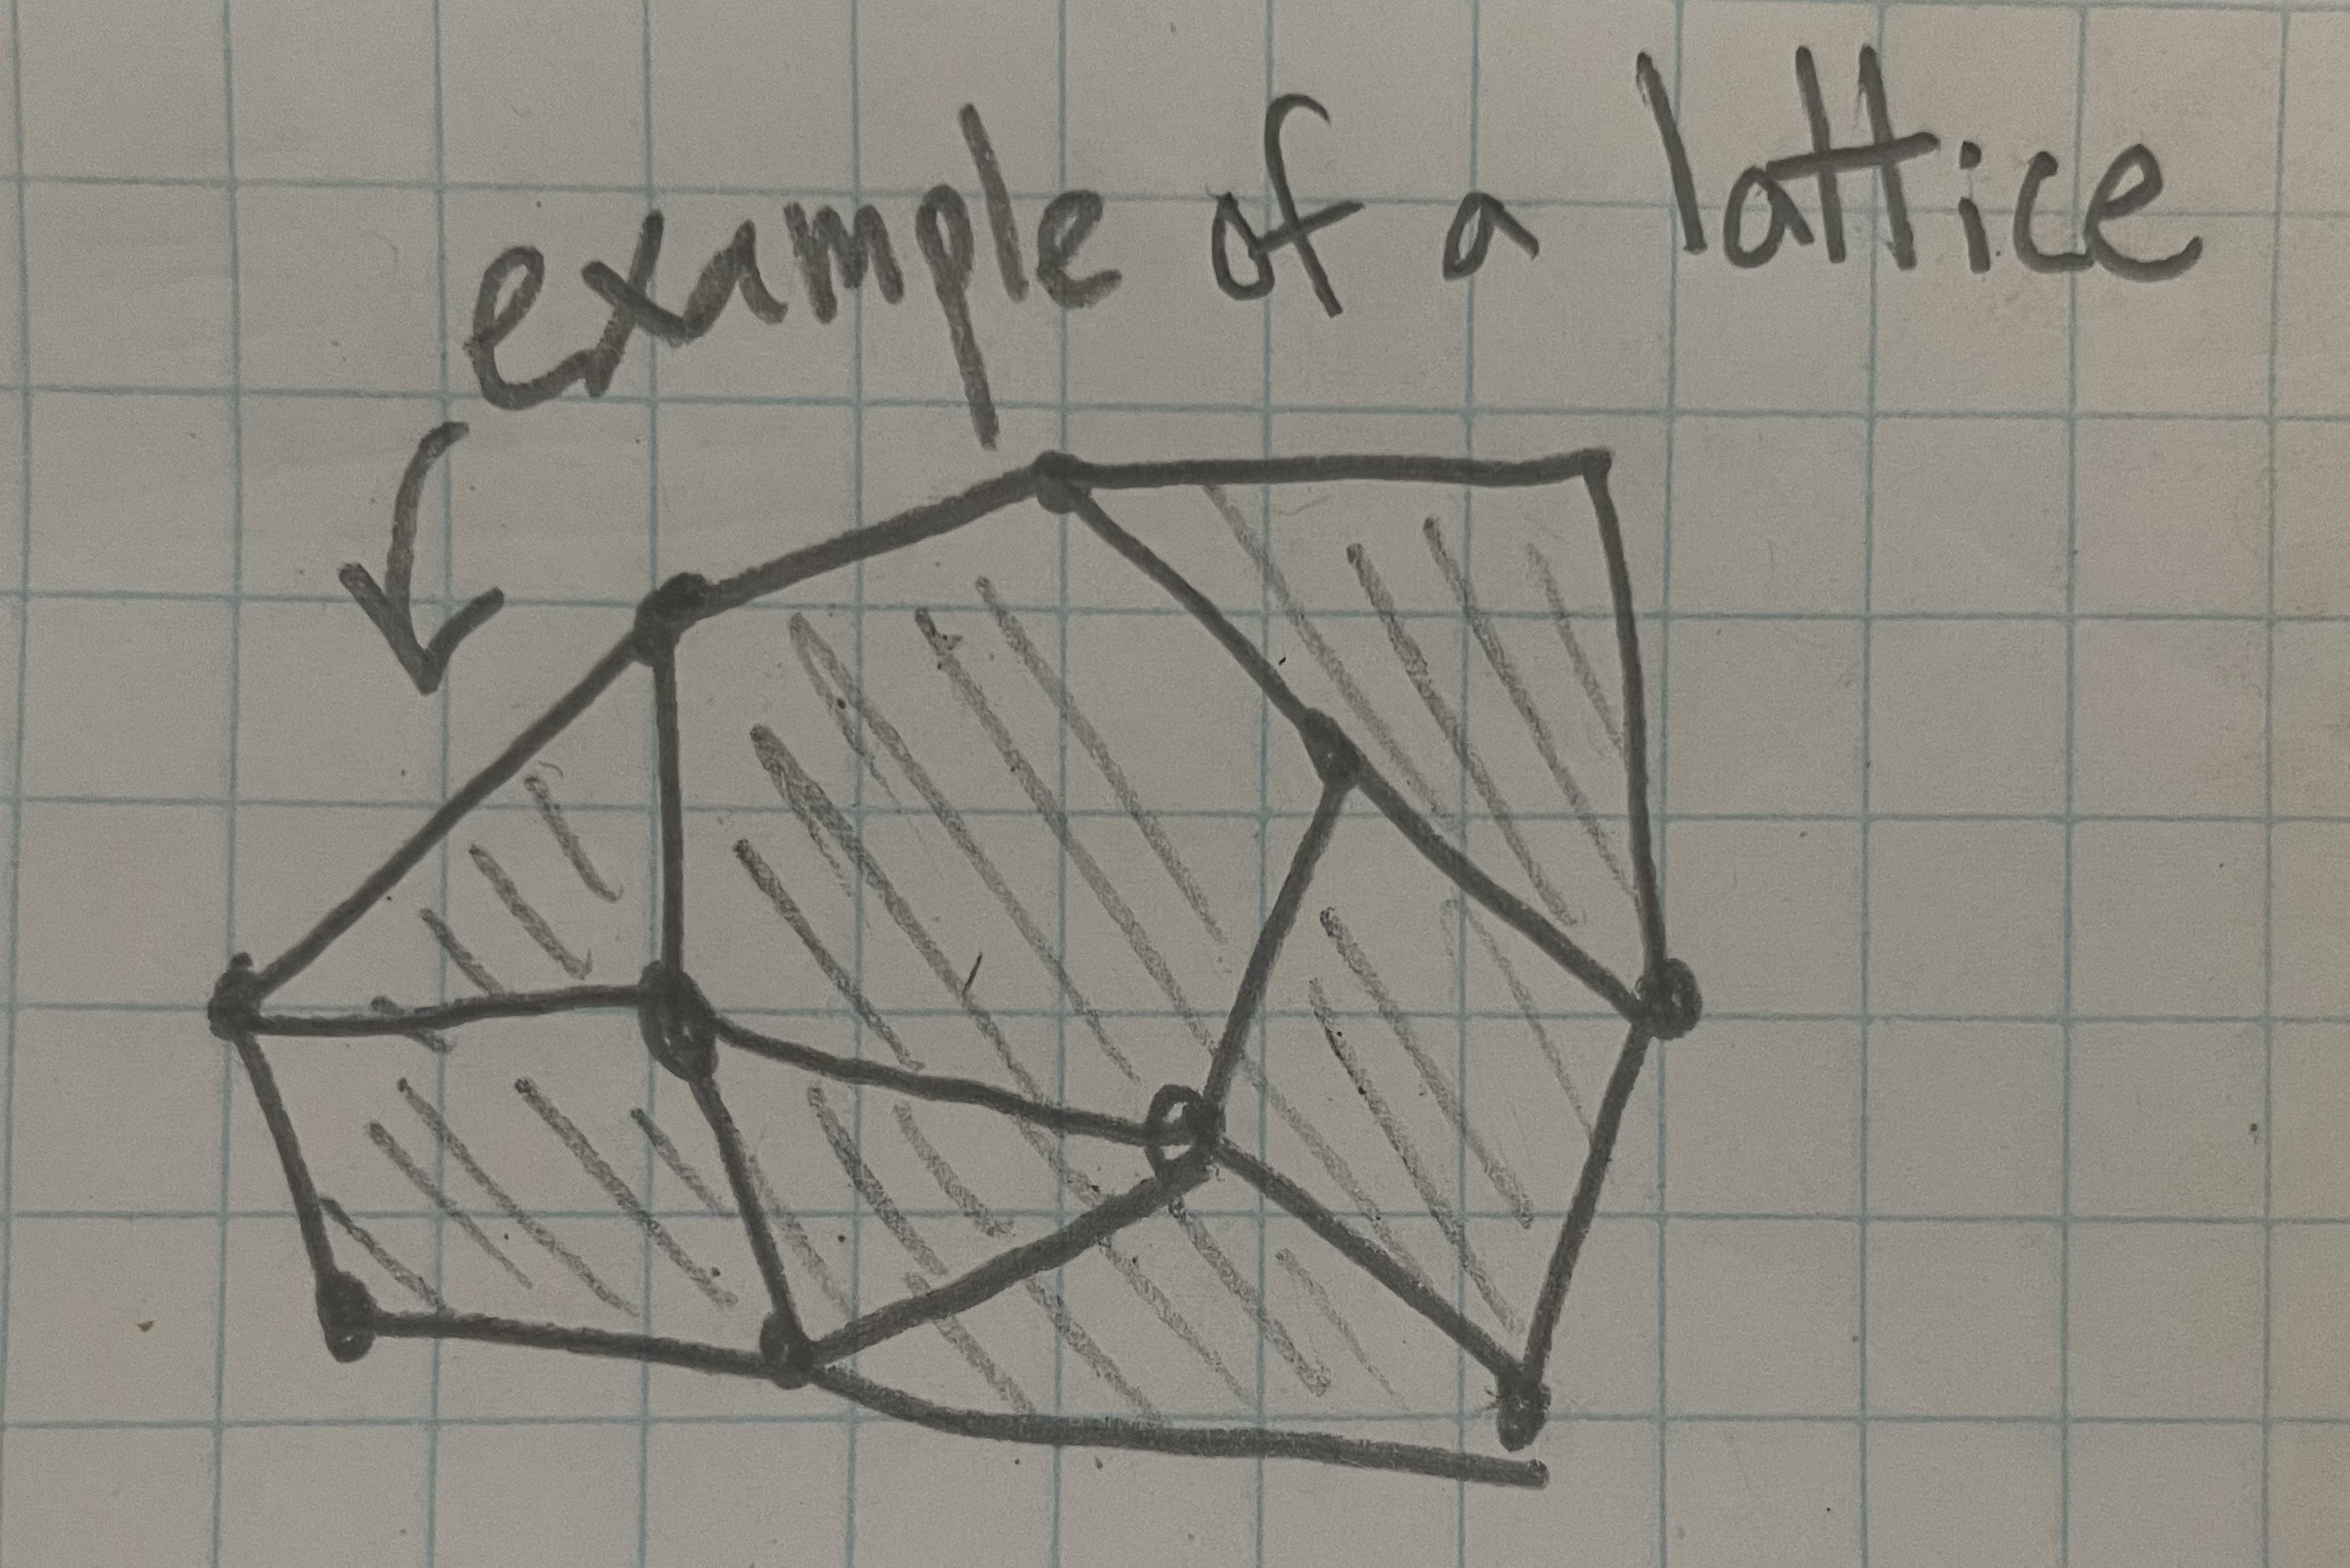
\includegraphics[scale=.04]{lattice-example}
\end{center}
\end{figure}

A lattice is a collection of vertices, edges, and faces connected in some way. To keep in line with the terminology common in topological quantum information, we refer to the faces of our lattices using the French term \textit{plaquette}. Formally, by lattice we mean ``simplicial 2-complex" though there is no need to go into details because we will never be dealing with the subtleties in the definition. Often times we will need to deal with \textit{directed} lattices. These are lattices in which every edge has a direction, which we represent as an arrow on that edge.

Before putting ordered media on a lattice, a good question is \textit{why} we would want to do this. There are two primary reasons. The first is that this will make this Hilbert spaces involved all finite dimensional. This is very important because we have only established quantum mechanics in the finite dimensional case, and working with the continuum limit can be highly complex. The second reason is that in practice, many of the systems physicists deal with are on lattices. For example, the chip of a quantum computer will store its information at finitely many sites, which can correspond to the vertices of some lattice. Many topological systems also arrise from materials which have crystal structures, which are modeled well by a lattice with atoms at the vertices and edges representing the geometry of the crystal.

The best setting for putting our ordered media on a lattice is by first putting on a torus. This helps for several reasons. Firstly, a torus is compact and hence it will add even more finiteness to the problem. Secondly, a torus has nontrivial topology which is useful for seeing the characteristic phenomina of topological order. Thirdly, a torus has no boundary, which helps because boundaries in topological order are subtle and require more work to describe. We denote the torus by $T^2$, and identify it with a square having its opposite sides glued:

\begin{figure}[h]
\begin{center}
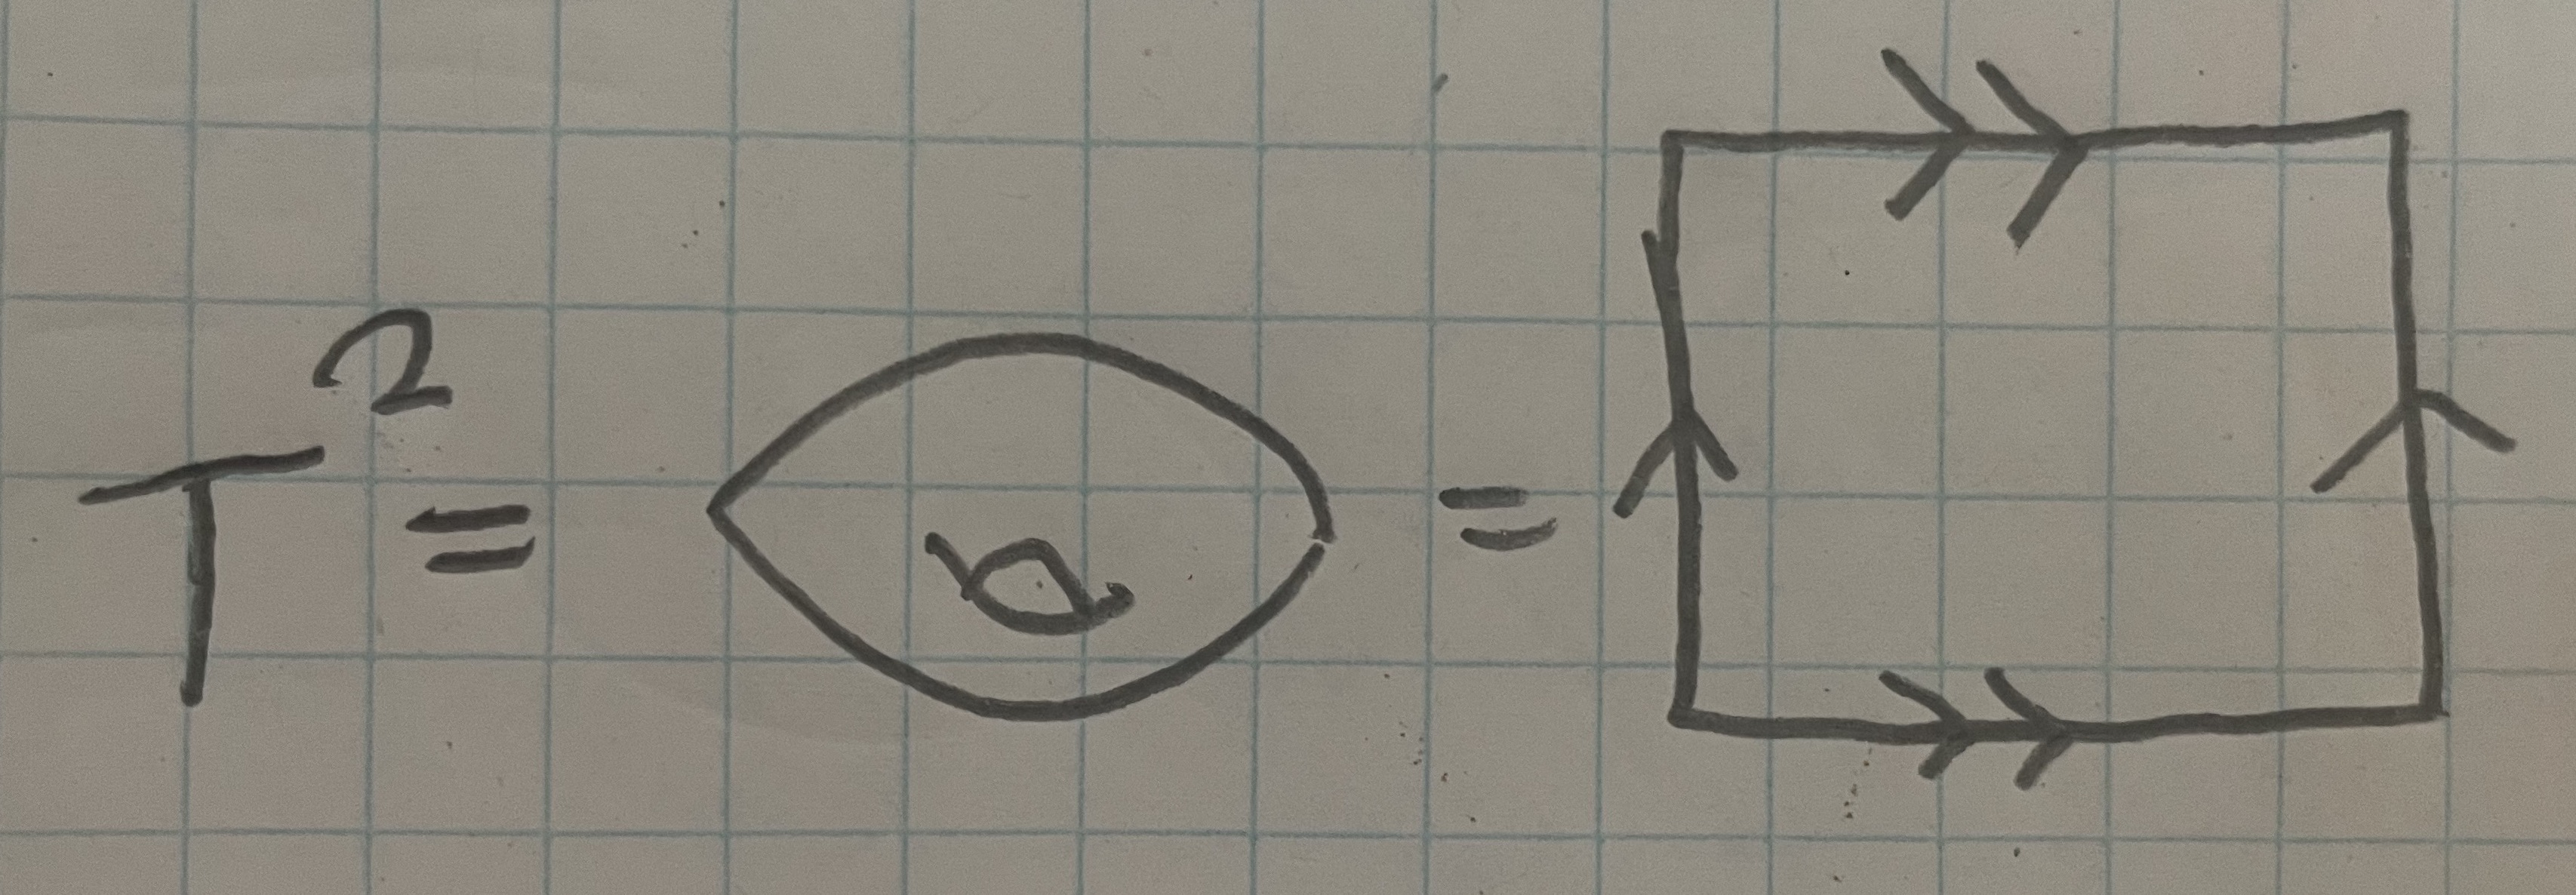
\includegraphics[scale=.04]{torus-definition}
\end{center}
\end{figure}

Ordered media on the torus corresponds to continuous maps $\phi: T^2\to M$ where $M$ is some fixed order space. The steps to transforming a state $\phi$ into a lattice version of itself go as follows:

\begin{enumerate}[Step $\text{1}$(a):]
\item Choose a directed lattice on the torus;
\item Choose a basepoint $m\in M$. Make \textit{local twists} around each vertex so that $\phi(v)=m$ for all vertices $v$ in the lattice.
\item On every edge, write down the winding number of $\phi$ along that edge, as an element of $\pi_1(M,m)$;
\item Forget $\phi$, and remember only the assignment of group elements in $\pi_1(M,m)$ to edges in the lattice.
\end{enumerate}

These steps deserve explanation. Step 1(a) is clear: we choose an arbitrary lattice on the torus. Typically we will choose the square lattice on the torus:

\begin{figure}[h]
\begin{center}
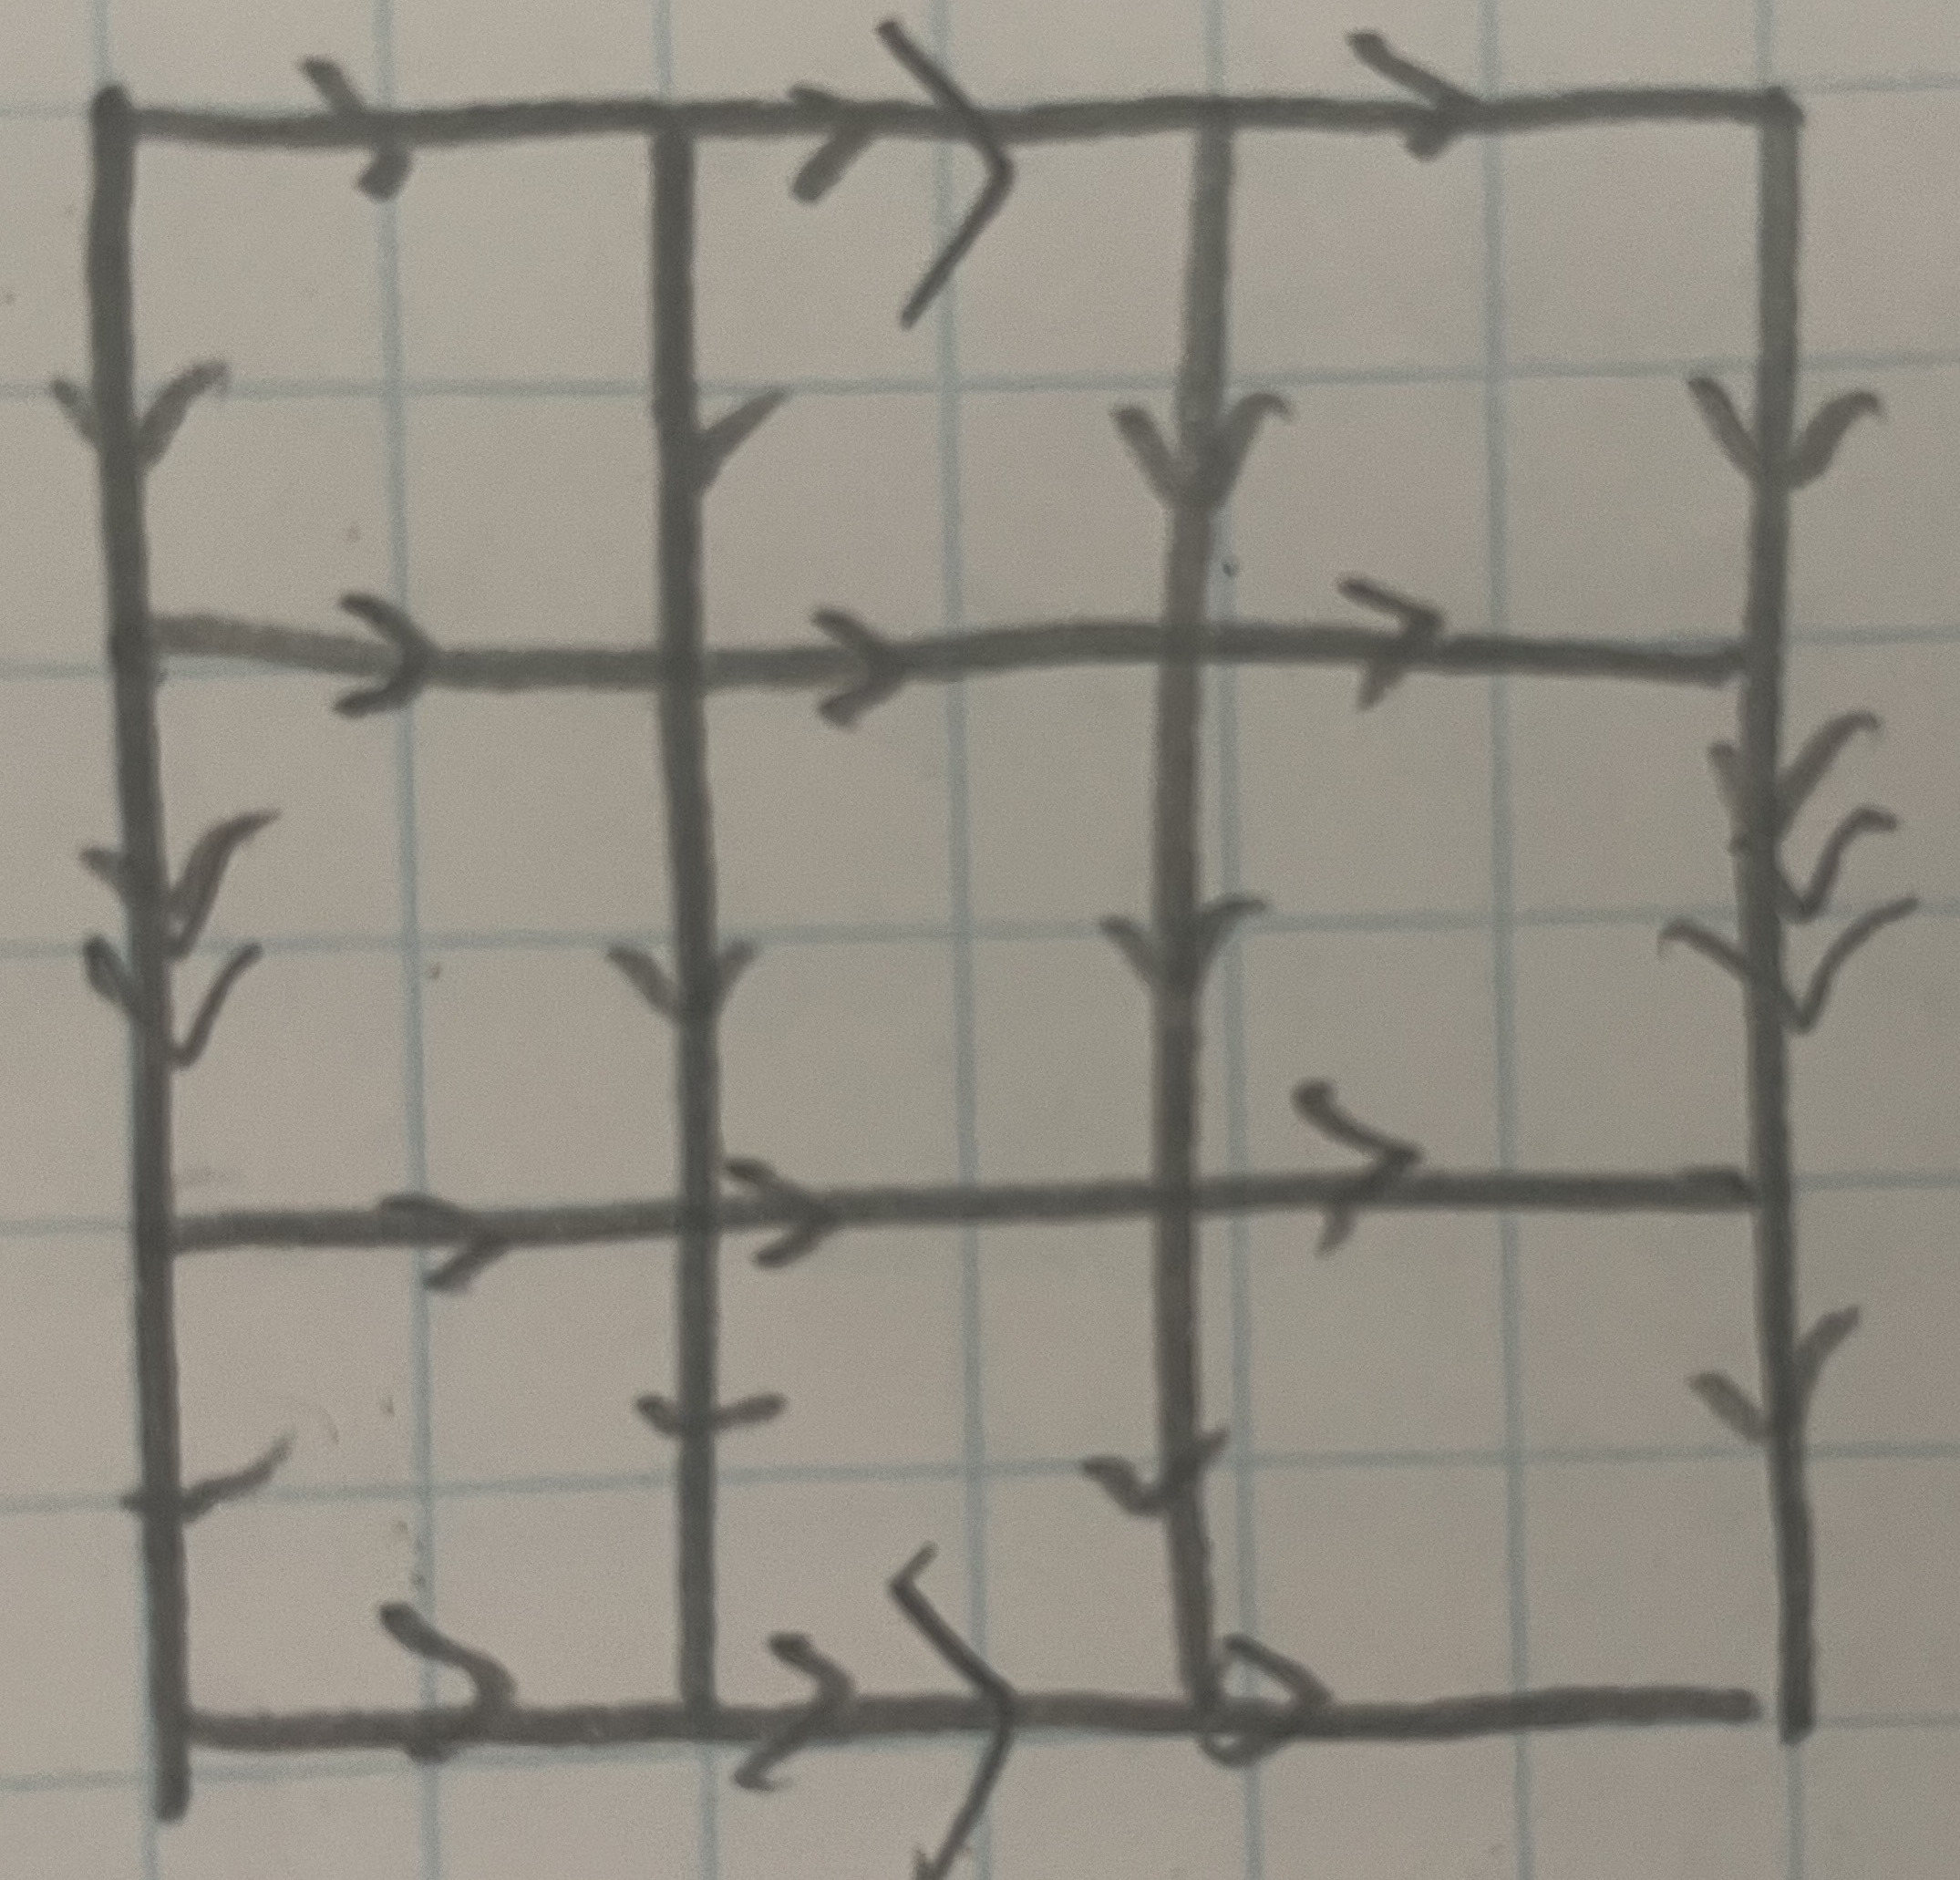
\includegraphics[scale=.04]{torus-lattice}
\end{center}
\end{figure}

Step 1(b) requires more explanation. The picture to imagine is that we take the state $\phi$ and twist its values in small neighborhoods around each vertex to enforce the condition $\phi(v)=m$. Formally, this means choosing another state $\tilde{\phi}$ such that $\tilde{\phi}(v)=m$ for every vertex $v$ of the lattice, and $\tilde{\phi}=\phi$ outside of some chosen small neighborhoods around each vertex. The fact that we can always choose such as state $\tilde{\phi}$ is a consequence of general mathematical principles in homotopy theory. Of course, different choices of $\tilde{\phi}$ will change the final result of our lattice encoding. However because any two choices of $\tilde{\phi}$ can only differ by local changes they can't be \textit{too} different, in a way we will quantify later in the subsection.

Step 1(c) is straightforward. Every edge can be thought of as a path. Pushing forward with $\phi$, this gives us a path in $M$. Since the edge starts and ends at vertices and $\phi$ sends all vertices to $m$, this means that the push forward of our edge gives a loop in $M$ based at $m$. Hence, it gives an element of $\pi_1(M,m)$. We can record this element and attach it as a piece of data associated to the edge.

Step 1(d) is entirely book keeping. It records the fact that we have successfully transformed our continuous data ($\phi:T^2\to M$) into discerete data (an assignement of group elements to edges in a lattice).

A worked example is shown below in the case that $M=S^1$ is the circle:

\begin{figure}[h]
\begin{center}
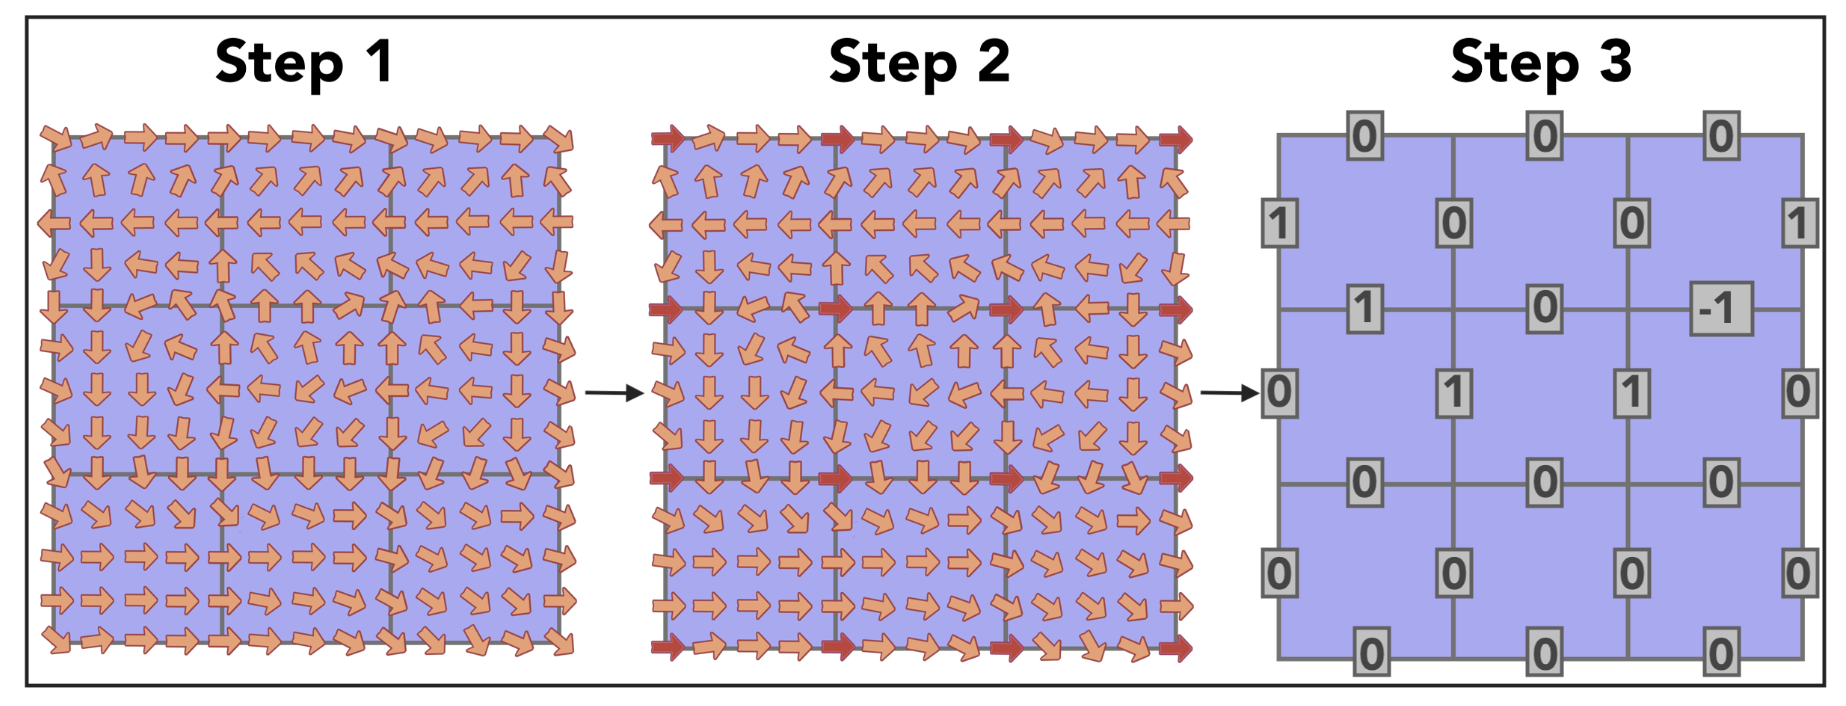
\includegraphics[scale=.3]{full-example}
\end{center}
\end{figure}

We now analyse our encoding of states in ordered media into assignements of group elements in $\pi_1(M,m)$ to edges in the lattice. The first fact from homotopy theory we will use is that these group elements determine the state $\phi$ exactly up to deformations localized within each face. Taking a limit of denser and denser lattices, this means that the group elements will specify $\phi$ up to increasingly local deformations. The intiution is that by taking an infinite lattice limit we should recover $\phi$ up to ``infinitely local deformations", i.e., we recover it exactly. In this way we did a good job with our lattice encoding.

We observe that not every assignement of group elements to edges appears in our construction. There are implicit conditions. In particular, imagine taking the product of the group elements on edges along some contractible loop, taking inverses appropriately so that all the arrows are pointing in the same direction. This product will be equal to the group element associated with the loop around this whole path. The winding number along any contractible path under a continuous map should be trivial. Hence, the product of these group elements should be trivial. In particular, given any plaquette, the ordered product of group elements along its edges should be zero:

\begin{figure}[h]
\begin{center}
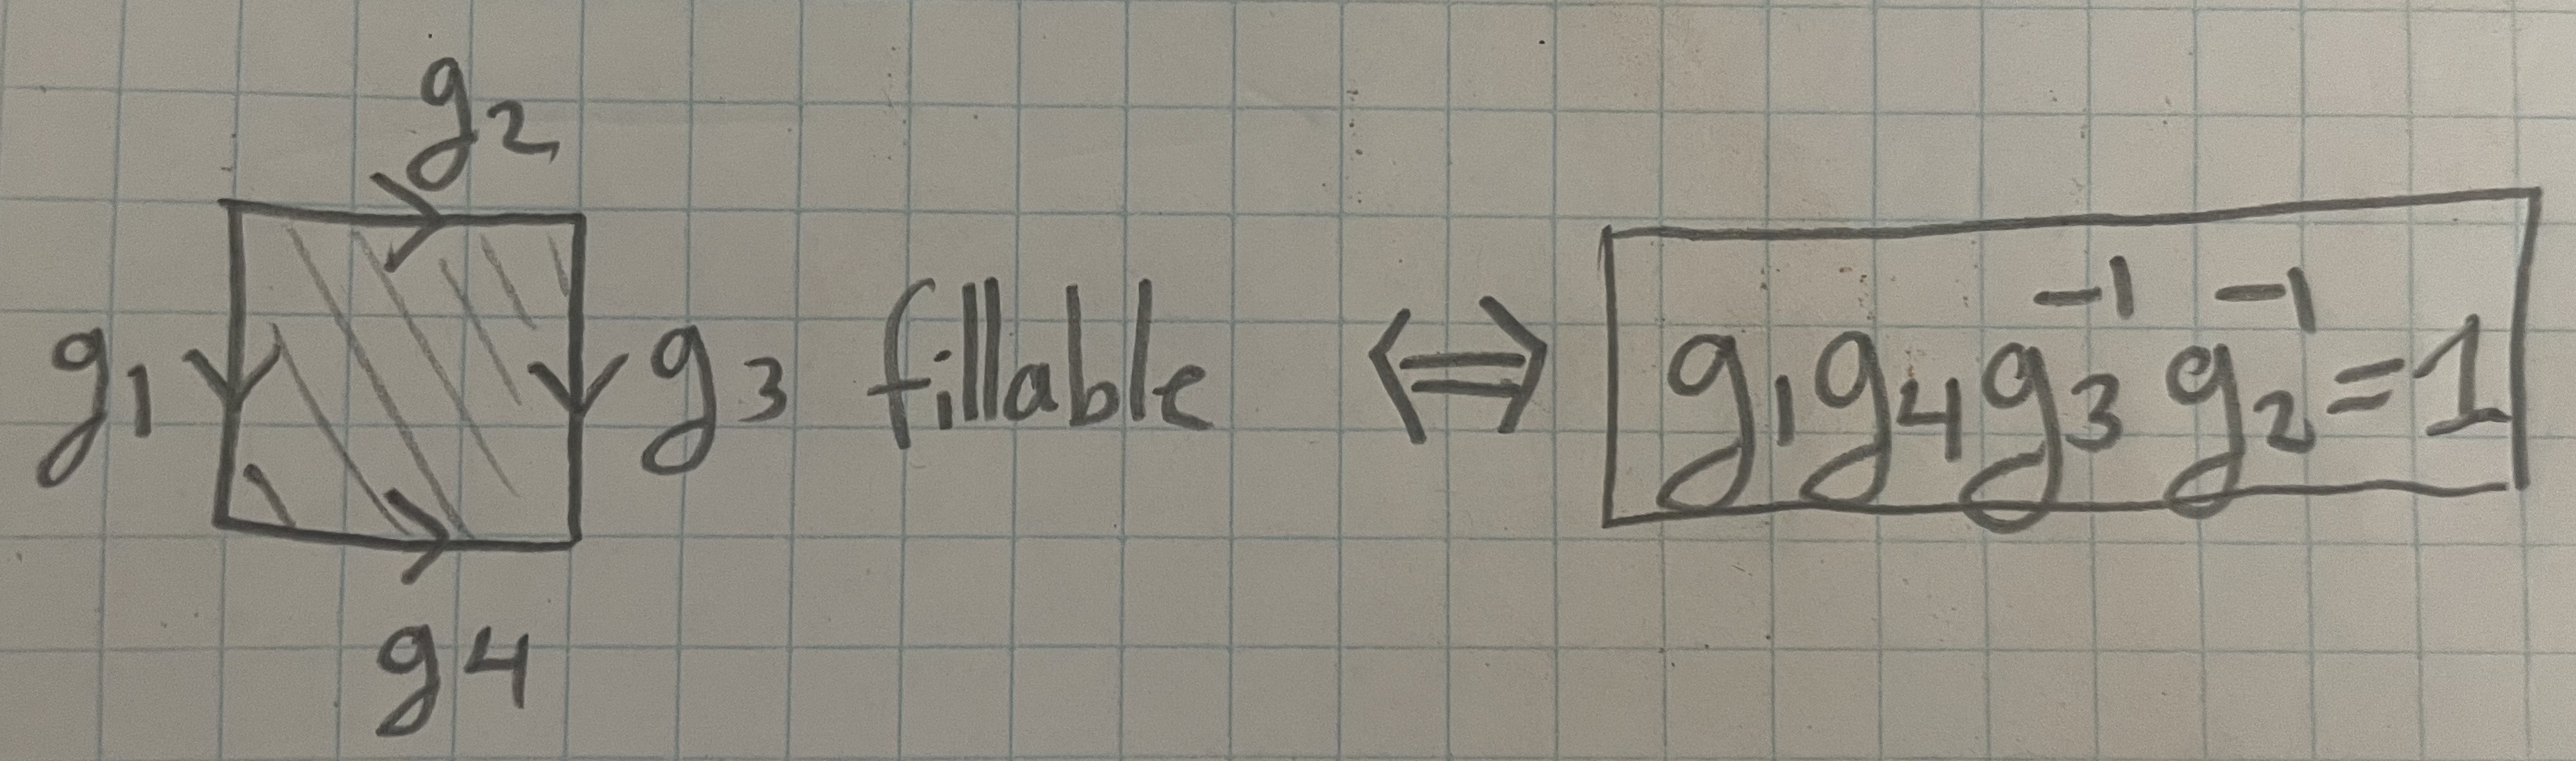
\includegraphics[scale=.06]{plaquette-rule}
\end{center}
\end{figure}

Moreover, \textit{any} coloring of the edges of the lattice by elements of $\pi_1(M,m)$ will come from some map $\phi$ so long as it satisfies the condition above. This is one of the key formulas of the theory. It is in a real sense a lattice version of the continuity condition, since it is \textit{equivalent} to the condition of continuity in the infinite lattice limit. This lattice version of continutity is called \textit{flatness}. Flatness conditions are the most common sort of compatibility conditions which appear when you have local degrees of freedom valued in some group, making this lattice situation very general.

The last thing do deal with in analysing our system is deformation. When analysing states in ordered media, a huge amount of our time was spent on performing continuous deformations. Topological information is defined to be information which is invariant under continuous deformation. What does this correspond to in the lattice model?

Suppose we are given an ordered media state $\phi$ and its corresponding lattice coloring. If we deform $\phi$ in some small neighborhood within a face, this will not change the values along the edges and hence will not change the coloring. If we deform $\phi$ in some small neighborhood around the interior of some edge this also won't change the coloring, because this will correspond to deforming the loop in $M$ induced by going along that edge, and elements of the fundamental group are invariant under deformations of this sort. Another way of seeing that the coloring can't change is that flatness must be preserved - if the group element on the deformed edge changed, it would ruin flatness on the faces it bounds.

Finally, we can consider deforming $\phi$ around some vertex. This certainly \textit{can} impact the coloring. An easy way to compute how it must impact the coloring is by using the fact that the flatness condition must be preserved. Suppose that an incoming edge labled by $g_1$ changes to $g_1 g$ after the deformation. Enforcing flatness along all of the faces touching the vertex allows one to conclude that all incoming edges $g_k$ will get changed to $g_k g$, and all outgoing edges $g_k$ will get changed to $g^{-1}g_k$, as shown below:

\begin{figure}[h]
\begin{center}
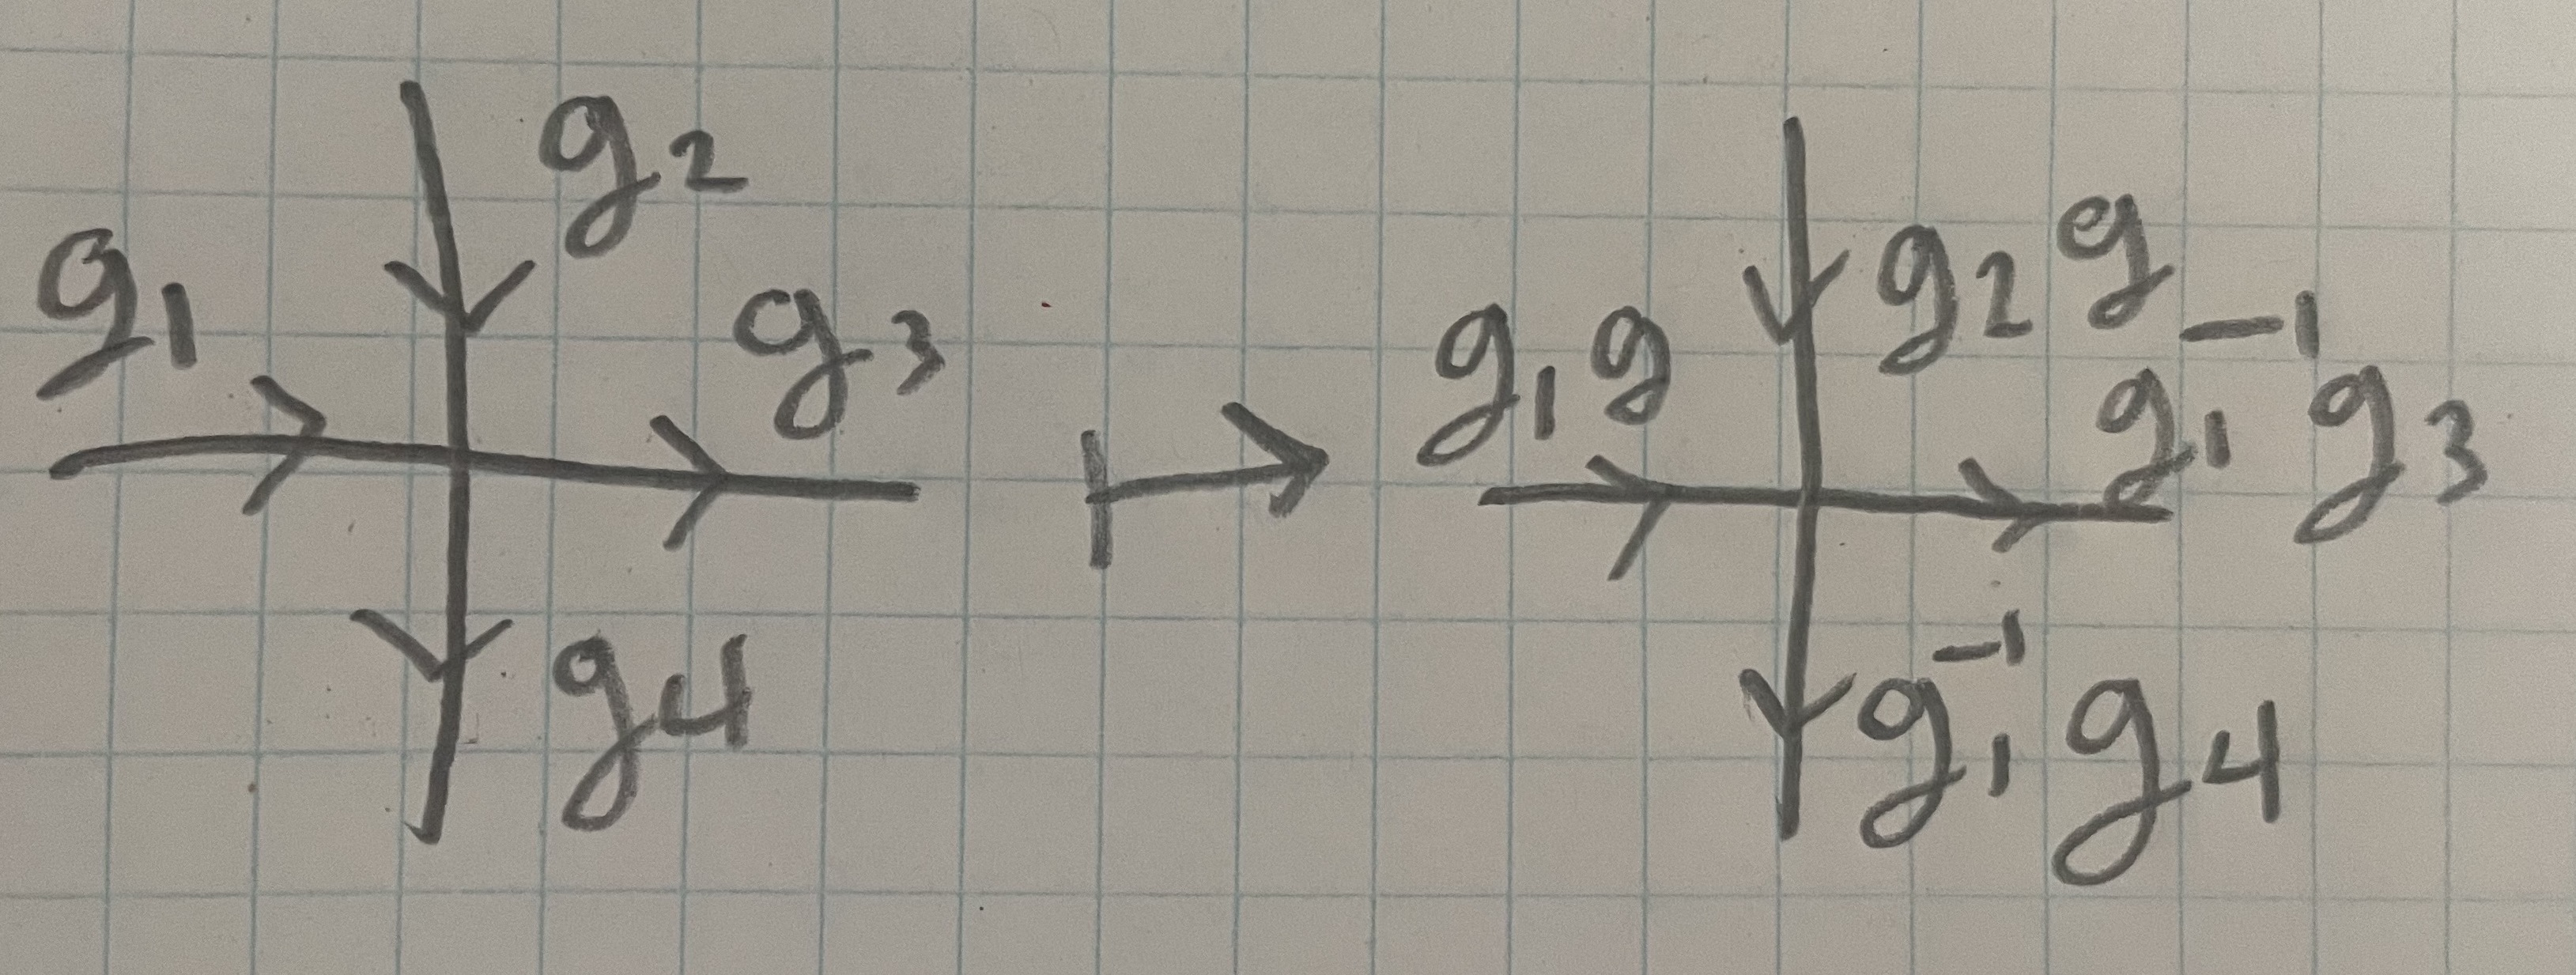
\includegraphics[scale=.04]{gauge-transformation}
\end{center}
\end{figure}

Another way of seeing this result is by anlysing what a deformation of $\phi$ does. The value $\phi(v)$ can move along some loop, starting and ending at $m$. This loop induces some element of the fundamental group, $g\in \pi_1(M,m)$. Performing this deformation exactly acts by precomposing/postcomposing the adject edges with $g$/ $g^{-1}$ accordingly. We can see below a concrete example for $G=S^{1}$:

\begin{figure}[h]
\begin{center}
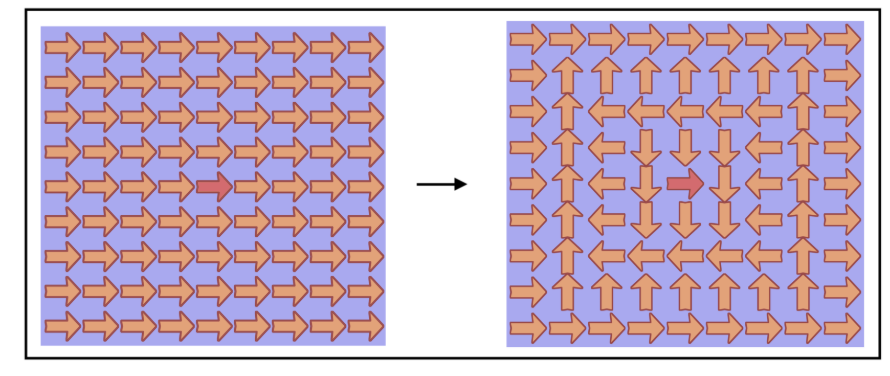
\includegraphics[scale=.45]{twisting}
\end{center}
\end{figure}

Hence, we have a picture for ordered media on the lattice: states correspond to flat colorings of elements of $\pi_1(M,m)$ on a fixed lattice, and continuous deformations correspond to certain vertex actions by elements of $\pi_1(M,m)$.

\subsubsection{From ordered media to gauge theory}

In the previous subsection we showed how to put ordered media on a lattice. In this section we show how to make it quantum, turning it from a classical field theory to a quantum gauge theory. The idea of this jump is as follows. In Section [ref] we obtained an equivalence

$$
\left(\substack{\text{topological information}\\ \text{in ordered media}}\right)=\left(\text{states}\right)/\left(\substack{\text{continuous} \\ \text{deformation}}\right).
$$

It is neccecary to mod out by continuous deformation because there is topoloigcal information in states, but also local degrees of freedom. For instance, the group element assigned to any indivudal edge in ordered media on a lattice can be changed by a gauge transformation and hence is not topologically invariant. The idea of going from ordered media to gauge theory is as follows: gauge theory is what results from ordered media when quantum fluxtuations become so strong that local degrees of freedom are completely washed out and only the topology remains.

The fluxtuations are quantum because we will imagine that our states will evolve in such a way that they are in a superposition of gauge transformations having been applied and not having been applied. Our states in gauge theory will be \textit{equal superpositions over all possible deformations} of a given state. In this way, we are using quantum mechanics as a physical mechanism for quotients. Equivalence classes under deformation will be physically realized as equal superpositions over all possible representatives.

This can all be made completely rigorous. Choose a lattice on the torus, an order space $M$, and a basepoint $m$. We define a Hilbert space

$$\NN=\bigotimes_{\text{edges}}\CC[G].$$

We canonically identify the standard basis of $\NN$ with $G$-colorings of the lattice. Let $C$ be an equivalence class of flat $G$-colorings of $\NN$ up to gauge transformations. There is a corresponding state

$$\ket{C}=\sum_{\gamma \in C}\frac{1}{\sqrt{|C|}}\ket{\gamma}.$$

This state is a normalized equal superposition of representatives of $C$. This defines a sub-Hilbert space

$$\Cc=\text{span}\left\{\left.\ket{C}\right| C\in \text{(flat $G$-colorings)}/\text{(gauge transformations)}\right\}.$$

This Hilbert space $\Cc$ stores the information in our gauge theory.

So far our system is relatively trivial - it is just a Hilbert space, with no Hamiltonian. We connect it back to our original picture of topological order. The space $\Cc$ is the collection of ground states in a topologically ordered system. Above it there is a whole spectrum of other states. This fuller picture with a Hamiltonian adds all of the subtlety and intrigue to the system.

In particular, we observed in Chapter [ref] section [ref] we observed the importants of quasiparticles in ordered media. These formed the heart of our information processing. Similarly, in gauge theory there will be quasiparticles as well which appear higher up in the spectrum of the Hamiltonian. Some of these quasiparticles will correspond to the classical quasiparticles in ordered media, but others are entirely new features of the system which did not exist before. We will analyse all this in more in the subsection that follows.

\subsubsection{Kitaev quantum double model}

[WORK: not sure if this is readable to someone who skipped the first two sections, but it should be. Something to keep an eye on.]

[WORK: Use $\D(G)$ as notation for the doubled quantum order associated to $G$.]

In this section we will give the Hamiltonian formulation of discrete gauge theory. Seeing as we have moved passed ordered media, we will no longer be working with order spaces and base points. Instead, we will choose an abstract finite group $G$ which replaces $\pi_1(M,m)$. The general picture for creating our Hamiltonian is simple, and follows a very general pattern in quantum theory: instead of enforcing properties rigidly as conditions, we will enforce them enforce properties energetically as terms in a Hamiltonian. The formulation we give below is known as the \textit{Kitaev quantum double model of discrete gauge theory}. It was introduced in Kitaev's seminimal paper on topological quantum information [ref]. It has been studied extensively in the literature by many authors [add more refs].

Choose a directed lattice on the torus. Let

$$\NN=\bigotimes_{\text{edges}}\CC[G]$$

be the HIlbert space of our quantum system. The space $\NN$ has a canonical basis given by $\prod_{\text{edges}}G$, which we  identify with $G$-colorings of the lattice. Given a $G$-coloring $\gamma$, we will denote the corresponding state in $\NN$ by $\ket{\gamma}$. For every plaquette $p$ in the lattice, we define an operator on $\NN$ by

$$B_p\ket{\gamma}=
\begin{cases}
\ket{\gamma} & \gamma \text{ flat at }p\\
0 & \text{otherwise}.
\end{cases}$$

We observe immediately that

$$\sum_{\text{plaquettes }p}(1-B_p)\ket{\gamma}=0 \iff \ket{\gamma} \text{ is flat.}$$

It is in this way that we can enforce properties energetically by adding them as terms to a Hamiltonian. If we chose the Hamiltonian to be $\sum_{\text{plaquettes }p}(1-B_p)$, then the lowest energy eigenspace would exactly correspond to the space spanned by flat $G$-colorings. For every vertex $v$ and group element $g\in G$, we define an operator on $\NN$ by

$$A_{v,g}\ket{\gamma}=\ket{\gamma \text{ acted on by the $g$ gauge action at $v$}}.$$

For any $\ket{\psi}\in \NN$, we call $\ket{\psi}$ \textit{gauge invariant at $v$} if $A_{v,g}\ket{\psi}=\ket{\psi}$ for all $g\in G$. We call $\ket{\psi}$ gauge invariant if it is gauge invariant at $v$ for all vertices $v$. We define

$$A_v=\frac{1}{|G|}\sum_{g\in G}A_{v,g}.$$

We define the Hamiltonian of our system to be

$$H=\sum_{\text{vertices $v$}}(I-A_v)+\sum_{\text{plaquettes $p$}}(I-B_p)$$

where $I$ is the identity operator. We summarize the basic properties of this Hamiltonian below:

\begin{proposition} The following properties of the Kitaev quantum double Hamiltonian hold:

\begin{enumerate}[(a)]
\item The operators $A_v$, $B_p$, and $H$ are Hermitian for all vertices $v$ and plaquettes $p$;
\item The formula $A_{v,g}^{\dagger}=A_{v,-g}$ holds for all vertices $v$ and $g\in G$;
\item All of the operators in the set $\{A_v,B_p\}_{v\in \text{vertices}, p\in \text{plaquettes}}$ commute with every other operator in the set;
\item The eigenstates of $H$ are simultaneous eigenstates of the operators $A_v$, $B_p$;
\item The eigenvalues of the $A_v,B_p$ are all $0$ or $1$;
\item The lowest eigenvalue of $H$ is $0$, and the $0$-eigenspace of $H$ is

$$\Cc=\text{span}\left\{\left.\ket{C}\right| C\in \text{(flat $G$-colorings)}/\text{(gauge transformations)}\right\}.$$

where for we define the ket

$$\ket{C}=\sum_{\gamma \in C}\frac{1}{\sqrt{|C|}}\ket{\gamma}$$

for any equivalence class $C$ of $G$-colorings of the lattice up to gauge transformations.

\end{enumerate}
\end{proposition}
\begin{proof}.[WORK: do proof]
\end{proof}

In particular, the above proposition tells us exactly that we have acheived our goal of realizing a Hamiltonian whose ground states capture the topological information in a lattice-version of ordered media.  The term ``double" in the Kitaev quantum double model refers to the fact that there are two families of terms in $H$ - one family of type $A_v$ and one family of type $B_p$. We can readily compute the dimension of the ground space as follows:

\begin{proposition} Choose a vertex $v$ in the lattice. Every $G$-coloring of the lattice induces an assignment of lattice loops on the torus based at $v$ to elements of $G$, based on taking the oriented winding number along that loop relative to the coloring. This restricts to a map

$$(\text{flat $G$-colorings})\xrightarrow{}\Hom(\pi_1(T^2,v), G)$$

where $\Hom(\cdot,\cdot)$ denotes the space of group homomorphisms between two groups. Any two flat $G$-colorings which differ by gauge transformations will induce the same map in $\Hom(\pi_1(T^2,v), G)$, up to global conjugation by an element of $G$. This induces a bijection

$$(\text{flat $G$-colorings})/(\text{gauge transformations})\xrightarrow{}\Hom(\pi_1(T^2,v), G)/\left(\substack{\text{simultaneous} \\ \text{conjugation}}\right).$$

The set of vectors ${\ket{C}}_{C\in (\text{flat $G$-colorings})/(\text{gauge transformations})}$ is linearly independent. Hence, there is a canonical isomorphism

$$\Cc \xrightarrow{}\CC[\Hom(\pi_1(T^2,v), G)/\left(\substack{\text{simultaneous} \\ \text{conjugation}}\right)]$$

given by taking winding numbers.
\end{proposition}
\begin{proof}.[WORK: give proof. I'm scared this could be too hard. It's already]
\end{proof}

The final step in using the above formula is to compute the fundamental group of the torus:

\begin{proposition} $\pi_1(T^2,v)\cong \ZZ^2$ for any vertex $v$. The two loops shown below are generators for $\pi_1(T^2,v)$:

\begin{figure}[h]
\begin{center}
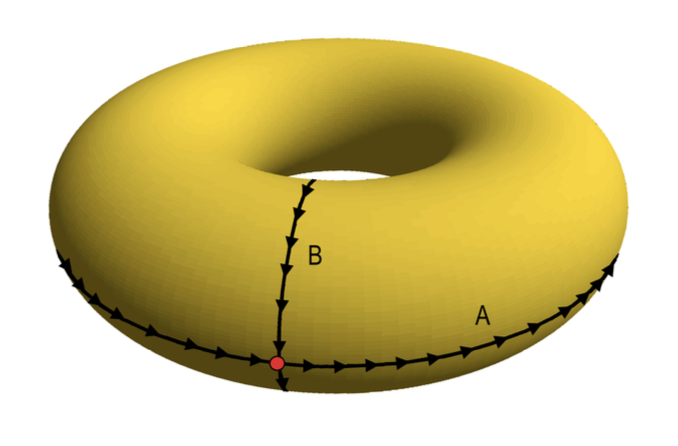
\includegraphics[scale=.3]{torus}
\end{center}
\end{figure}

\end{proposition}
\begin{proof}.[WORK: proof]
\end{proof}

One last observation to make about this ground space is that its ground states really are globally different:

\begin{proposition} Let $L$ be length of the shortest non-contractible loop on the lattice. Let $\gamma_0,\gamma_1$ be non-gauge equivalent flat $G$-colorings of the lattice. There are at least $L$ edges at which $\gamma_0$ and $\gamma_1$ assign different values.
\end{proposition} 
\begin{proof}.[WORK: do proof]
\end{proof}

In particular, if we choose the square lattice on the torus, then the length $L$ of the shortest non-contractible loop is obvioulsy a good measure of linear system size. Proposition [ref] tells us that the number of local changes requires to go from one ground state to another is on the order of $L$. This is exactly the sort of condition we needed in Section [ref] to conclude topological protection in the ground states. Of course, the smallest non-zero eigenvalue of $H$ is at least $1$, which is bounded away from zero and hence there is a system-size independent gap between the ground states and the other states. Hence, we see that $H$ is a good topologically ordered Hamiltonian. 

The excited states of $H$ will be described localized excitations with quasiparticle behavior. Given a state $\ket{\psi}\in \NN$, we will say that a state has an \textit{excitation at vertex $v$} if $A_v\ket{\psi}=0$ and we will say that is \textit{unnoccupied at $p$} if $A_v\ket{\psi}=1$. We say that $\ket{\psi}$ has an \textit{excitation at plaquette $p$} if $B_p\ket{\psi}=0$ and that it is \textit{unnocupied at $p$} if $B_p\ket{\psi}=1$. By Proposition [ref], every energy eigensate is either occupied or unoccupied at every vertex/plaquette. The regions in which $\ket{\psi}$ is unnoccupied are all essentially identical, leading to a homogenous bulk. The sites at which $\ket{\psi}$ is occupied are different, and behave as quasiparticles. We will define operators which move these excitations around.

[WORK: Add something about local indistinguishability of ground states - reinforce this ``homogenous bulk" idea.

More than this, it is important to note that earlier we are giving a rigorous definition of topological order. It is not immediately obvious that the KQDM satisfies this definition. This is the main content of the paper \cite{cui2020kitaev}. Should I include a proof? At the very least there should be some mention of how this fits into the definition. In fact, this should be a big point. The KQDM is being introduced with the main goal of giving an example of TO. Needs to talk about how it is topological.]

[WORK: Maybe also reinforce that this could be done on \textit{any manifold}, and the gound states would be the same? ]

\subsection{The toric code}

[WORK: Maybe this section can be re-done. We know that the total space $\NN$ can be decomposed as a direct sum

$$\NN=\bigoplus_{\lambda}\NN_\lambda$$

as a direct sum over syndromes, by general principles of diagonalizable matrices. To prove that all of the $\NN_\lambda$  have an even $\#$ of excited terms in $H$ of both $A_v$ and $B_p$ type is easy. Proving that they all have the same dimension involves the simple observation that applying $\sigma_X$ and $\sigma_Z$ between two excited terms will make them both ground states. Simple counting recovers the fact that the ground state is $4$-dimensional.

The beauty of this approach is that it is immediately grounded. We have a Hamiltonian, we want to solve it - i.e. we want to compute the dimensions of the $\NN_\lambda$, and explicitely have a way of creating those basis states. The proof in a real sense is using the quasiparticle nature of the $A_v$ and $B_p$ excitations. Namely they are being moved along paths to annhilate with one another.

Every operator can be decomposed as a sum of Pauli operators. Hence, unerstanding how Paulis act on $\NN$ lets understand how every operator acts on $\NN$. Paulis act on $\NN$ by creating/moving/fusing vertex/plaquette excitations. Hence, understanding vertex/plaquette excitations tells you everything you need to know about the toric code. Saying it this way makes everything feel very grounded, and it doesn't bring in anyons unnececarily early into the picture. We can talk about anyons after. Highlight the fact that they behave like quasiparticles and that they will become objects of independent interest, but that isn't the point yet.

]

\subsubsection{Simplified Hamiltonian}

In this section we move on to analyzing the Kitaev quantum double model for $G=\ZZ_2$, which is known as the \textit{toric code}. The name toric code comes from the fact that the toric code was first introduced as an error correcting code, and was only later recast as a topologically ordered system [refs]. The toric code is still the basis for many of the most popular error correcting codes [refs]. In a real sense the toric code is the simplest nontrivial topological order. It is a fantastic example which demonstrates almost all of the phenomina of topological order with relatively little work involved. The toric code, and more generally $\ZZ_2$ discrete gauge theories, can be found in all sorts of systems such as [WORK: give examples]. 

We describe the model now. Because $G=\ZZ_2$ is abelian, we will switch to additive notation for our group operation. We choose a \textit{non-oriented} lattice structure on the torus. This lattice does not need to be oriented because changing the direction of edges in the lattice corresponds to taking inverses, and $g=g^{-1}$ for every element $g\in \ZZ_2$. We define

$$\NN = \bigotimes_{\text{edges}}\CC[\ZZ_2]=\bigotimes_{\text{edges}}\CC^2.$$

Here, we identify $\CC[\ZZ_2]$ with $\CC^2$ for convenience, endowing $\CC^2$ with a canonical basis $\{\ket{0},\ket{1}\}$. We call $\CC^2$ a \textit{qubit}, in analogy to ``bits" for classical computing. It is a standard two-level quantum system. Most quantum computers are based on qubits, which makes the toric code especially accessable to practical implementation as an error correcting code. The definition of the Hilbert space $\NN$ can be summarized as putting a qubit on every edge of the lattice. The Hamiltonian is

$$H=\sum_{\text{vertices }v}(1-A_v)+\sum_{\text{plaquettes }p}(1-B_p).$$

We unpack the general definitions of $A_v$ and $B_p$ for the toric code. The operator $A_{v,0}$ is the identity. The operator $A_{v,1}$ acts by a gauge transformation,

\begin{figure}[h]
\begin{center}
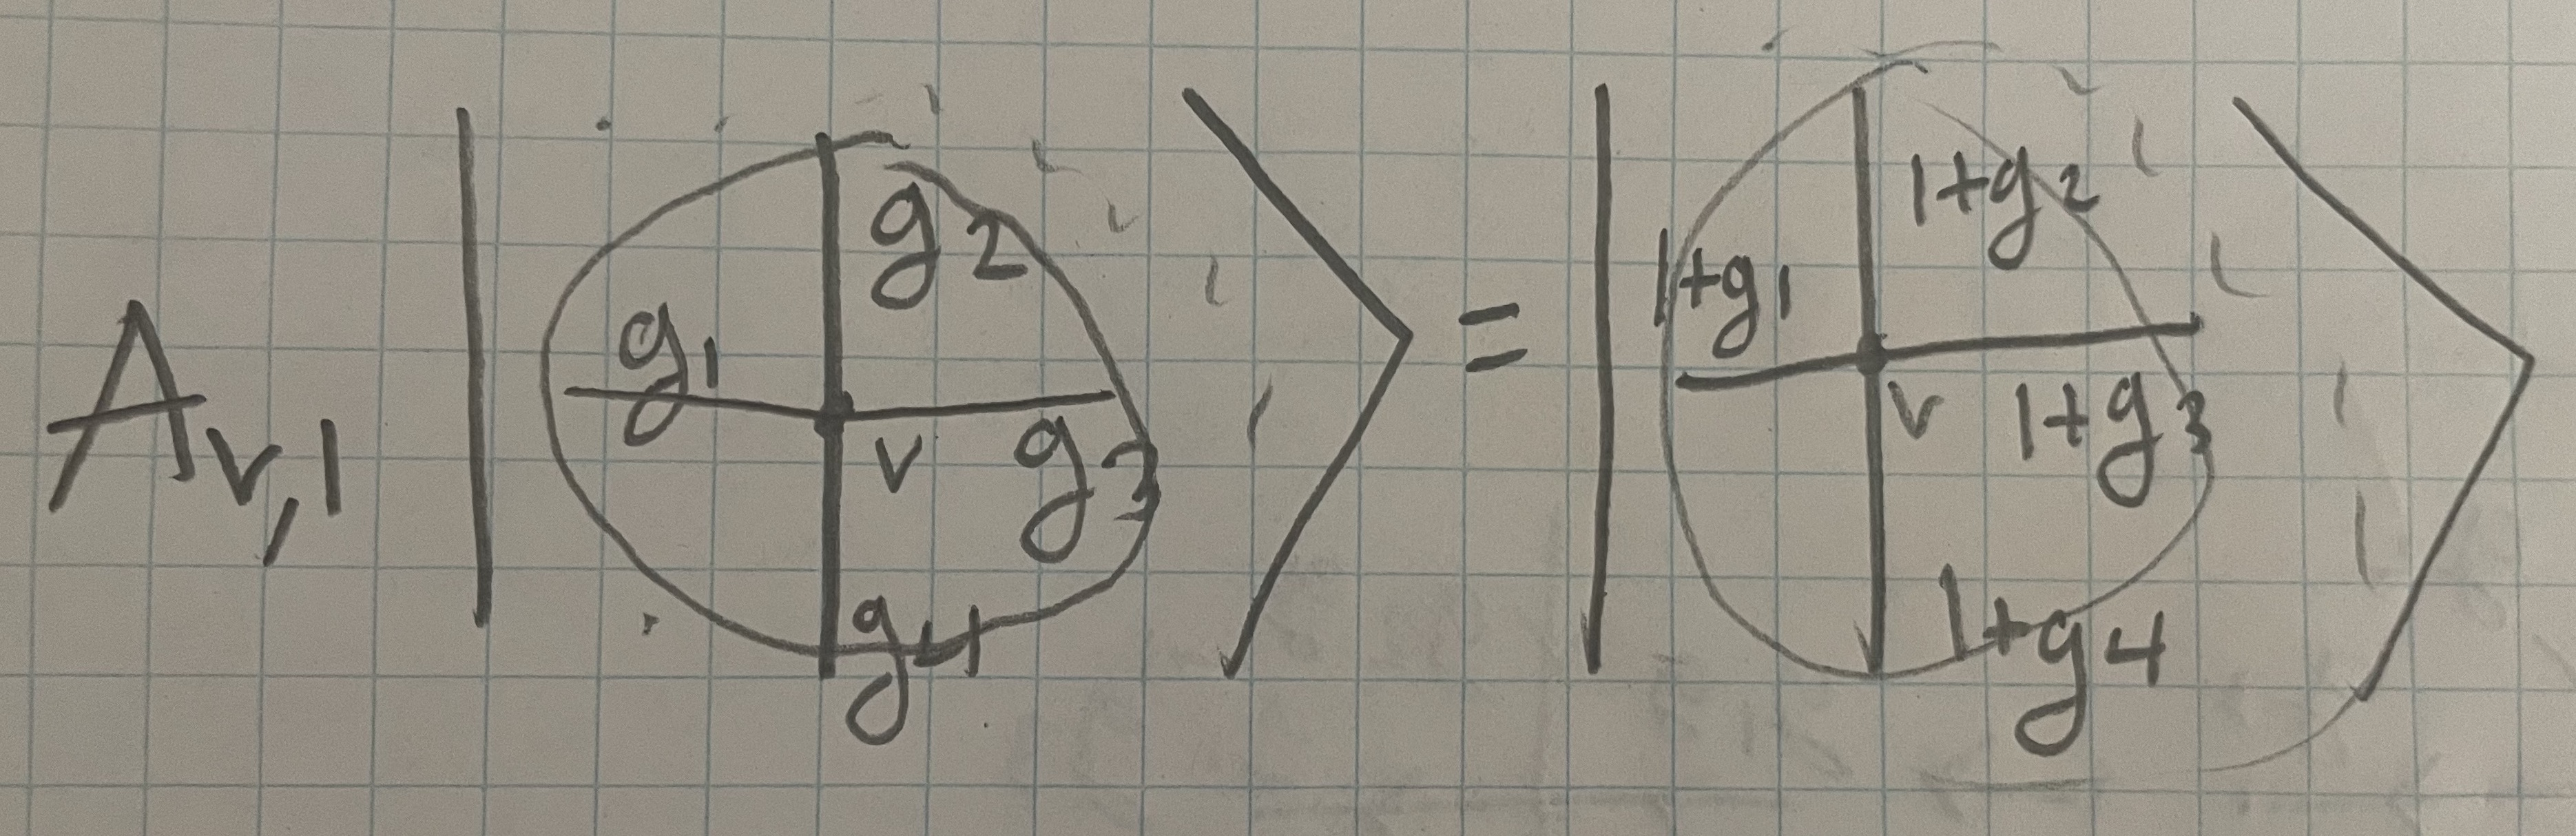
\includegraphics[scale=.04]{Av-gauge-action}
\end{center}
\end{figure}

Defining

\begin{align*}
\sigma_X:\CC^2&\xrightarrow{}\CC^2\\
\ket{0}&\mapsto \ket{1}\\
\ket{1}&\mapsto \ket{0}
\end{align*}

we thus find that

\begin{align*}
A_{v,1}=\bigotimes_{\substack{\text{edges} \\ \text{touching }v}}\sigma_X, && A_v=\frac{1}{2}\left(I + A_{v,1}\right).
\end{align*}

Moving on to $B_p$, we recall that

\begin{figure}[h]
\begin{center}
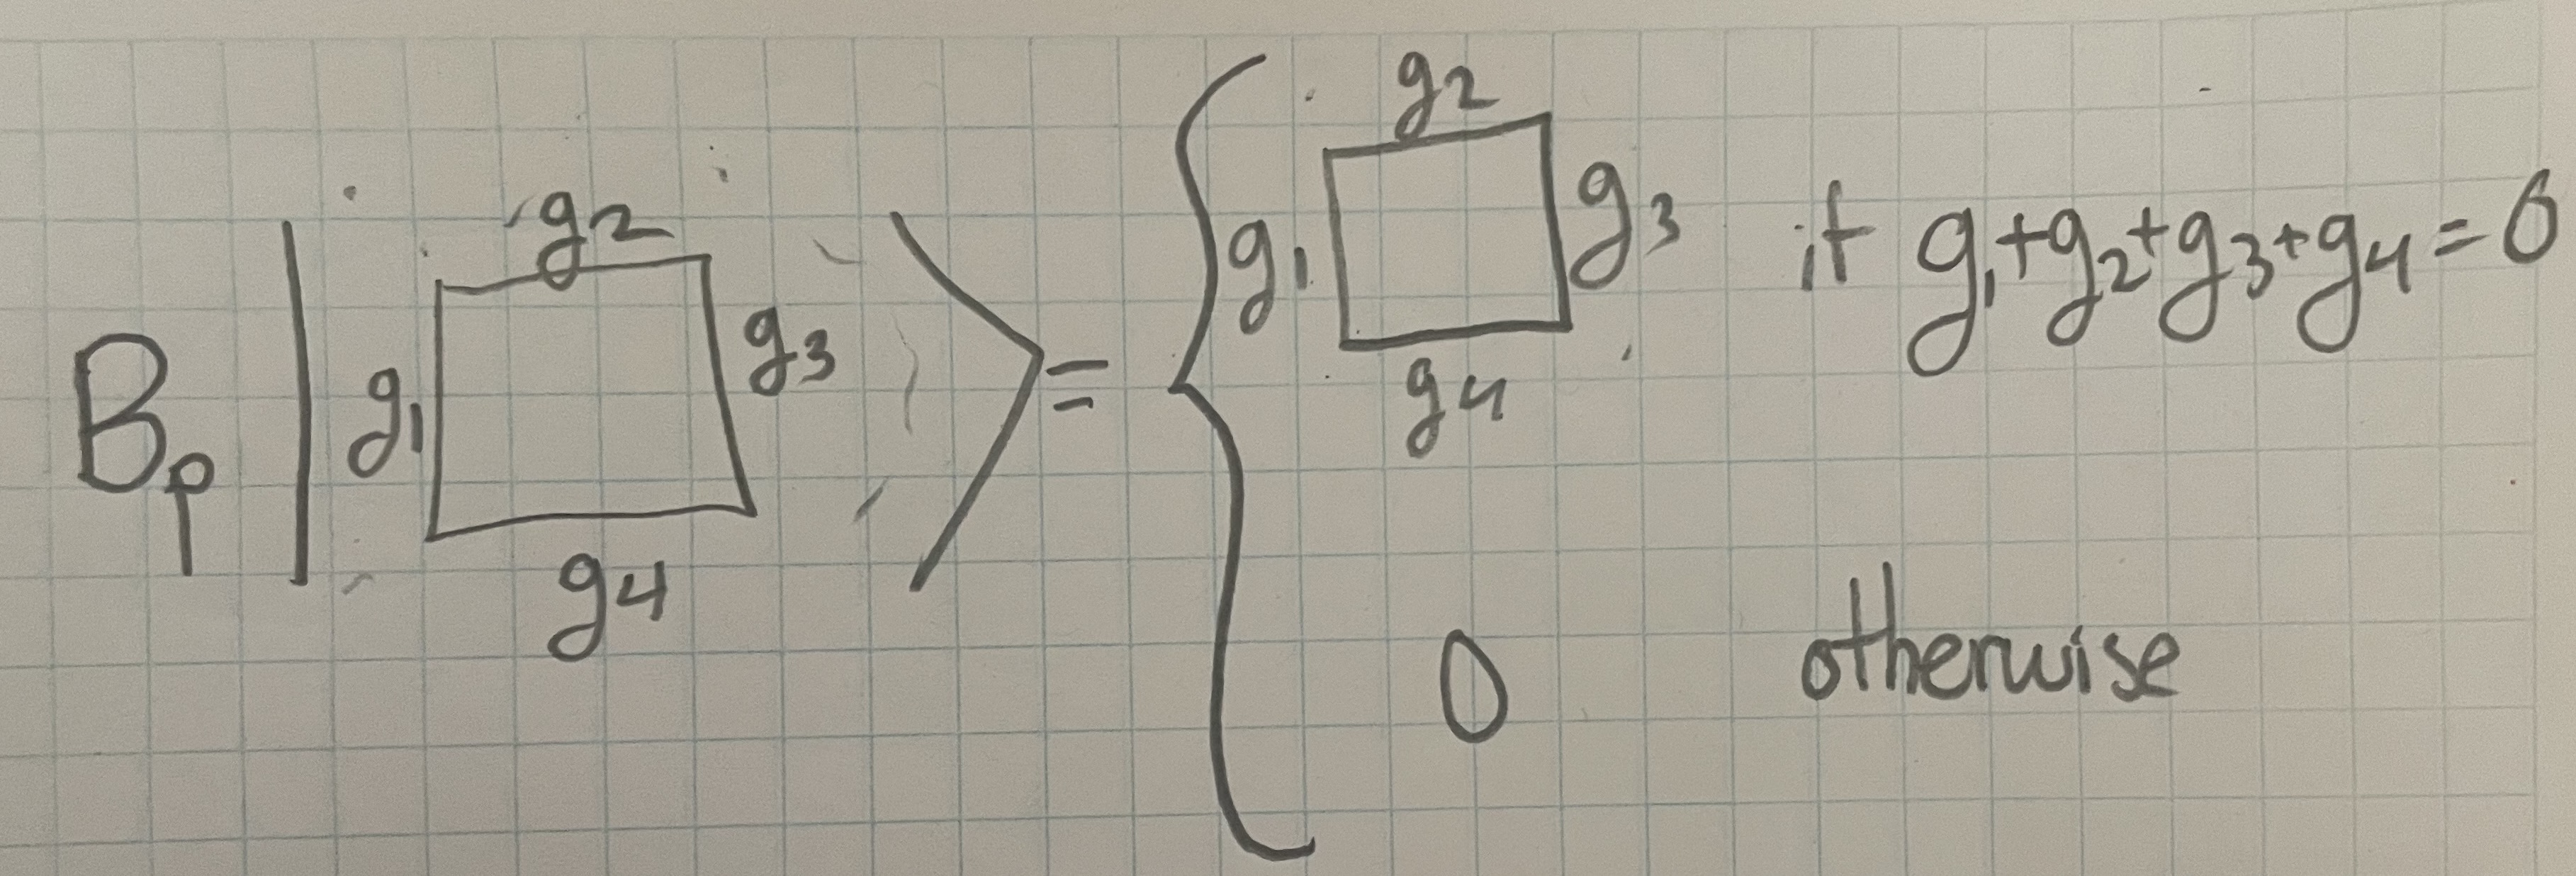
\includegraphics[scale=.04]{Bp-definition}
\end{center}
\end{figure}

In the present case, $B_p$ has a more workable expressing that is symmetric to our description of $B_p$. Define

\begin{align*}
\sigma_Z:\CC^2&\xrightarrow{}\CC^2.\\
\ket{0}&\mapsto \ket{0}\\
\ket{1}&\mapsto -\ket{1}
\end{align*}

Philosophically, it is useful to interpret $\sigma_Z$ as acting as $\ket{g}\mapsto \chi(g)\ket{g}$ where $\chi:\ZZ_2\to\CC^\times$ is the unique nontrivial character of $\ZZ_2$, $\chi(0)=1$, $\chi(1)=-1$. Since $\chi$ is a group isomorphism, for any $g_1,g_2,g_3,g_3\in G$ we have an equivalence

$$g_1+g_2+g_3+g_3=0 \iff \chi(g_1)\chi(g_2)\chi(g_3)\chi(g_4)=1.$$

Defining an auxillary $B_{p,1}$, we thus find the following expression for $B_p$:

\begin{align*}
B_{p,1}=\bigotimes_{\substack{\text{edges} \\ \text{bounding }p}}\sigma_Z, && B_p=\frac{1}{2}\left(I + B_{p,1}\right).
\end{align*}

For simplicity, we will often rewrite the Hamiltonian as

$$H=\frac{1}{2}\sum_{\text{vertices }v}(1-A_{v,1})+\frac{1}{2}\sum_{\text{plquettes }p}(1-B_{p,1}).$$

The matrices $\sigma_X$ and $\sigma_Z$ we defined are known as \textit{Pauli matrices}. They are extremely common across formulae in quantum mechanics - this is another reason that the toric code is so ammenable to error correction applications. The basic properties of these matrices are summarized below:

\begin{proposition}$\,$
\begin{enumerate}[(a)]
\item The operators $\sigma_X$ and $\sigma_Z$ are simultaneously unitary and Hermitian;
\item $\sigma_X^2=\sigma_Z^2=I$;
\item $\sigma_X \sigma_Z = - \sigma_Z \sigma_X$;
\end{enumerate}
\end{proposition}
\begin{proof}.[WORK: do proof]
\end{proof}

An important thing to note is that $A_{v,1}$ and $B_{p,1}$ commute, despite the fact that $\sigma_X$ and $\sigma_Z$ anticommute. The fact that they commute follows from Proposition [ref], though it fruitful to reavulate that proposition in this present context. The important fact is that given any vertex $v$ on the exterior of any face touching $p$,  there are an \textit{even number} of edges which both touch $v$ and bound $p$. Hence, the number of tensor factors in which $A_{v,1}$ and $B_{p,1}$ anticommute is even, and hence overall they commute.

The last step in reinterpreting our general theory of Kitaev quantum double models to the toric code is computing the ground space. We observe that since $\ZZ_2$ is abelian acting by conjugation does nothing, and hence

$$\Hom(\pi_1(T^2,v), \ZZ_2)/\left(\substack{\text{simultaneous} \\ \text{conjugation}}\right)=\Hom(\pi_1(T^2,v), \ZZ_2).$$

Seeing as we are no longer modding out by conjucation, the group operation on $\ZZ_2$ extends to a group operation on $\Hom(\pi_1(T^2,v), \ZZ_2)$. Hence this space forms an abelian group, which we denote

$$H^1(T^2,\ZZ_2)=\Hom(\pi_1(T^2,v), \ZZ_2)=(\text{flat $\ZZ_2$-colorings})/(\text{gauge transformations}).$$

[WORK: maybe set notation and write out four elements explicitely? Might be too much.]

This is the \textit{cohomology group of $T^2$ with coeffecients in $\ZZ_2$}. Since $\pi_1(T^2,v)\cong \ZZ^2$, we conclude that

$$H^1(T^2,\ZZ_2)\cong \ZZ_2^2.$$

Hence, we obtain the following:

\begin{proposition} The $0$-eigenspace of $H$ is four dimensional. It is spanned by the vectors

$$\ket{C}=\frac{1}{\sqrt{|C|}}\sum_{\gamma\in C}\ket{\gamma}$$

for $C\in H^1(T^2,\ZZ_2)$.
\end{proposition}
\begin{proof}.[WORK: do proof]
\end{proof}

\subsubsection{Exact solution of the toric code}

When given a quantum system, the first thing to do with it is to \textit{solve it}. This means diagonalizing the Hamiltonian. In this case of the toric code, the diagonalization of $\NN$ is the direct sum decomposition

$$\NN = \bigoplus_{E\in \RR}\NN_{E}$$

where $\NN_{E}$ is the energy $E$ eigenspace,

$$\NN_{E}=\{\ket{\psi} | ,\, H\ket{\psi}= E \ket{\psi}\}.$$

Solving the toric code amounts to explicitely describing $\NN_E$ for each $E$. In particular, this means computing the dimension of each space. The Hamiltonian for the toric code is 

$$H=\sum_{v}(1-A_v)+\sum_{p}(1-B_p).$$

Since the $A_v$ and $B_p$ all commute with each other, they are \textit{simultaneously diagonalizable}. This is a huge help in our analysis. We introduce some notation to take advantage of this insight. We define a \textit{syndrome} on the toric code to be a map

$$\lambda: (\text{faces})\sqcup (\text{vertices})\xrightarrow{}\{\pm 1\}.$$

We define the syndrome $\lambda$ subspace of $\NN$ to be

$$\NN_{\lambda}=\{\ket{\psi}\in \NN | \,\, A_{v,1}\ket{\psi}=\lambda(v)\ket{\psi},\,\, B_{p,1}\ket{\psi}=\lambda(p)\ket{\psi}    \forall v,p\}$$

We define the energy $E_{\lambda}$ of a syndrome $\lambda$ by the formula

$$E_{\lambda}=\sum_{v}\frac{1}{2}(1-\lambda(v))+\sum_{p}\frac{1}{2}(1-\lambda(p)).$$

The fact that the operators $A_v$, $B_p$, and $H$ are simultaneously diagonalizable is codified in the following observations:

\begin{proposition} We have that

\begin{align*}
\NN = \bigoplus_{\text{syndromes $\lambda$}} \NN_{\lambda}, && \NN_{E}=\bigoplus_{\substack{\text{syndromes $\lambda$}  \\ E_\lambda = E }  } \NN_{\lambda}.
\end{align*}

\end{proposition}
\begin{proof} This follows immediately from the above discussion.
\end{proof}


We can now solve the toric code:

\begin{proposition} We have that

\begin{equation*}
\dim(\NN_{\lambda}) = 
\begin{cases}
4 & \text{if }\prod_{v}\lambda(v) = \prod_{p}\lambda(p) = 1\\
0 & \text{otherwise.}
\end{cases}
\end{equation*}

\end{proposition}
\begin{proof}.[WORK: do proof]
\end{proof}

\begin{corollary} We have that

$$\dim (N_{E})=[WORK: write\,\, formula]$$
\end{corollary}
\begin{proof} . [WORK: do proof]
\end{proof}

[WORK: this section will have some commentary about how Pauli operators are being used to fuse $X$-type and $Z$-type excitations. The way this commentary sounds should depend on the way the proof looks. I might want to include this lemma before the proof:

Given an edge $e$ in the lattice and an operator $U:\CC^2\to \CC^2$, denote by $(U)_e:\NN\to\NN$ the operator which applies $U$ on the tensor factor of $\CC^2$ at edge $e$. We compute the following:

\begin{lemma} For any vertex $v$, edge $e$, plaquette $p$, we have

\begin{align*}
A_v  (\sigma_X)_e=(\sigma_X)e A_v, && B_p (\sigma_Z)_e=(\sigma_Z)e B_p,
\end{align*}

\begin{equation*}
A_v (\sigma_Z)_e=
\begin{cases}
- (\sigma_Z)_e A_v & \text{if $e$ touches $v$}\\
(\sigma_Z)_e A_V & \text{otherwise}
\end{cases}
\end{equation*}

and

\begin{equation*}
B_p (\sigma_X)_e=
\begin{cases}
- (\sigma_X)_e B_p & \text{if $e$ bounds $p$}\\
(\sigma_X)_e B_p & \text{otherwise}
\end{cases}
\end{equation*}


\end{lemma}

]

\subsubsection{Toric code as a topologically ordered system}

.[WORK: prove that toric code satisfies axioms of TO.]

[WORK: This section will really dig into how the Pauli algebra acts on states]

[WORK: this section can also show that \textit{global} errors (e.g. $\sigma_X$ all the way around a torus) acts non-trivially. Maybe give a proof? Make a little quantum computer? If I do, I should reformulate it in in the ``adiabatically changing Hamiltonian" way to tie it into the way I talked about it in the introduction.]



\subsection{Anyons}

\subsubsection{Topological quantum information in excited states}

Let us recap our current picture of topological quantum information. We introduced topological order, and argued as a general principle that its ground states are invariant under local deformations. That is, if we start with a ground state in a topologically ordered system, apply some local operator, and then project back onto ground states, then we will get back to the state we started with up to some phase. This lets us store information in ground states. This information can be used as a place to store stable information, and can be acted on by global operators to perform computations such as in proposition [ref].

We now take this perspective to its logical extreme. The dimension of the ground state space depends only on the topological order of the system and the global topology of the physical space. For instance, toric code topological order on a torus will always have a four dimensional ground space, independent of system size or choice of microscopic lattice.

To make a computer, however, we need to be able to store arbitrarily large amounts of information. This means that either we will need to work with increasingly complex topological orders or increasingly complex surfaces. There are only a handful of topological orders known to be physically realizable, so working with increasinlgy complex topological orders is out of the question. Hence, once needs to work with increasingly complex surfaces. By working on high-genus surfaces, the ground state space can be made as large as possible. This gives the following picture for a topological quantum computer:

[WORK: add picture, a-la Freedman et al.]

This approach is potentially possible, and we will explore it more in section [ref]. However, no matter the implimentation it adds a great deal of complexity. Adding genus onto a computer chip is hard work. It would be much better to work with a state with the least complex topology possible, preferably a plane, sphere, or torus.

It is for this reason that we turn to a key idea in the theory of topological order: \textit{being careful, it is possible to store topologically protected information in the excited states of a topologically ordered system}.

[WORK: picture of spectrum diagram, with excited states boxed. ``Use these to store information!"]

Using the excited states of a topologically ordered system to store information comes with several obstacles:

\begin{enumerate}
\item It requires careful study. This isn't a fundamental problem, but it is relevant to us since we are about to embark on that study;
\item It requires a more powerful control over the topologically ordered system than working only with ground states. This can make the approach impossible in some physical systems;
\item It introduces non-topological local degrees of freedom. This non-topological information needs to be worked around so that proper fault-tolerant computations can be performed.
\end{enumerate}

We now recall our procedure for storing information in ground states. The key point is that we have a projector $\PP:\NN\xrightarrow{}\NN_{g.s.}$. This projector satisfies the relation that $\PP \OO \PP = \lambda\cdot \PP$ for any local operator $\OO$, for some $\lambda\in \CC$. Our physical picture for topological quantum computing is that we are continually measuring with respect to $\PP$, and hence constantly projecting into the ground space. The formula $\PP \OO \PP$ says that even if noise is applied between rounds of projection it is okay because our state will only change by a phase and hence will still store the same information.

[WORK: try $\PP_{E}$ onto states of a fixed energy. Problem: drift. Solution: constrain drift. Anyons!]




\subsubsection{Definition}

We haven't mentioned them by name yet, but \textit{anyons} are one of the key concepts in the theory of topological quantum information. This is so much true that our algebraic theory of topological quantum information is in reality a theory of anyons. It is a nontrivial fact that describing anyon behavior is enough to recover the rest of topological quantum information. So, before going to the algebraic picture, it behooves us to get very clear on what anyons are, how they behave, and why they are important.

\begin{definition} An \textit{anyon} is a localized excitation in a topologically ordered system.
\end{definition}

Let's unpack this definition. To be concrete we work first in the Kitaev quantum double model based on a finite group $G$.

For our first picture of anyons we will ignore global topology. This means either working on an infinite plat plane or on a small region in some large sphere or torus. By definition our anyon must be \textit{localized}. In physics, we say that a phenominon is localized if it is constrained to some compact domain which is small relative to system size.

An excited state is by definition a state which has high energy, that is, a state which is not a ground state. A state hosts a localized excitation within a region if it is a ground state outside of that region, and only has high energy within the region. This gives the below picture of an anyon:

[WORK: add picture.]

Formally, given a compact region $R$, we say that a state $\ket{\psi}$ of the Kitaev quantum double model \textit{hosts an anyon} in $U$ if $A_v\ket{\psi}=B_p\ket{\psi}=\ket{\psi}$ for all $v,p\not\in U$.

More generally, a state could host multiple anyons. Given a finite set $R_1.... R_n$ of compact connected regions, we say that $\ket{\psi}$ hosts $n$ anyons at $R_1$, $R_2$,... $R_{n-1}$ and $R_n$ if $A_v\ket{\psi}=B_p\ket{\psi}=\ket{\psi}$ for all $v,p\not\in \bigcup_{i=1}^nR_i$.

[WORK: add picture of three anyons on the torus.]

Of course, with this definition it is not impossible for the physical space to be entirely covered with anyons, as shown below:

[WORK: open cover on the torus.]

In this case the anyon picture is not very useful. Every state $\ket{\psi}$ can be viewed as a ground state covered uniformly with anyons. The idea is that at low temperatures the anyon picture will become more useful. At low temperuatres the energy $E$ of the system will be bounded above indenpendent of system size. This means that $A_v\ket{\psi}\neq \ket{\psi}$ and $B_p\ket{\psi}\neq \ket{\psi}$ at a bounded number of different sites $v,p$. Hence, at low temperatures and large system sizes all realistic states $\ket{\psi}$ can be modeled as a large homogenous bulk with a small number of anyons.

Clearly, anyons are localized regions of differences in a homogenous bulk. Moreover, we see that some operators can create and move anyons. For instanece, let $\OO:\NN\to\NN$ be linear operator. Given any state $\ket{\psi}$, the operator $\O$ can change the anyon content of $\ket{\psi}$:

[WORK: write out the three cases

\begin{itemize}
\item Move anyon;
\item Create anyons;
\item Annhilate anyons;
\end{itemize}

This is also a good place to introduce the term \textit{local operator}. It is clear that local operators can only change anyon content in a bounded region, and only by a bounded amount. This means that local operators work well with the anyon picture.

This above observation makes anyons behave as \textit{quasiparticles}. Manipulating these anyonic quasiparticles allows for topological quantum computing in a style similar to what was described in section [ref]. I should say a few words about this.
]

[WORK:

Talk about this in the toric code. Vertex and plaquette failiures give anyons. $\sigma_X$ and $\sigma_Z$ can act as operators to move, create, and annhilate anyons. I should mention and include this in this section, before going any further.
]



[WORK: So far I haven't defined what an anyon is for topological orders other than the KQDM. One easy way to do this is by putting some set $L$ of sites, choosing $d>0$, defining $\NN=\bigotimes_{\ell \in L}\CC^d$. Then we have $H=\sum_{i}H_i$, $[H_i,H_j]=0$, $H_i^2=1$, $H_i$ localized to some region $U_i$. This is a commuting local projector Hamiltonian. It is easy to define anyons in a model like this one. I'm not sure if this would be informative or distracting.]


\subsubsection{Principles of anyons}

Now that we have defined anyons, its good to take the time to talk about the general principles which guide them. The most important of these principles is their \textit{braiding}. We demonstrate this with anyons in the toric code. Suppose that we move an $Z$-type anyon around a $X$-type anyon, in some state $\ket{\psi}$. This amounts to applying $\sigma_Z$ operators in a square around a plauqette:

[WORK: add picture.]

Here we observe something amazing. The operator used to move the $Z$-type anyon around the $X$-type anyon is $\bigotimes_{\text{edges touching $p$}}\sigma_Z$. This operator is exactly $B_{p,1}$! Hence, by the fact that there is a $X$-type anyon at $p$, we conclude that $B_{p,1}\ket{\psi}=-\ket{\psi}$ and thus moving the $Z$-type anyon around the $X$-type anyon resulted in a phase of $-1$.

Suppose that we performed a similar experiment in three dimensional space. We got two particles, and moved one around the other. Clearly, this trajectory can be continuously deformed into the trajectory of doing nothing:

[WORK: add picture.]

Hence, moving two particles around each other must act by the identity. Formally, the state-space of a two particle system will be some vector space $V_2$. The action of moving one particle around the other is some unitary operator $V_2\to V_2$. In three dimensional space, this opearator must be the identity.

Hence, we have found something fantastic. The behavior of anyons in (2+1)D space is fundamentally different than the behavior of particles in (3+1)D space.

The fact that there could theoretically be quasiaprticles in (2+1)D space in which moving one particle around another acts nontrivially was first theorized in [ref]. It was later in [ref] that Wilczek discovered that the FQHE could host anyons, and thus these exotic particles could be realized in the laboratory.

The possibility for anyons in (2+1)D space is especially exciting when it is contrasted with how constrained braiding statstics are in (3+1)D space. Consider some particle in (3+1)D space. We consider the swap map, exchaning two copies of the particle. When this swap map is repeated twice, we get a braid identitcal to moving one particle around the other. Hence, swapping twice gives the identity. Denoting the Hilbert space of the two particle system by $V_2$, a-priori the swap map $\swap:V_2\to V_2$ could be any operator which squares to one. However, subtle topological and algebraic considerations revealt that $\swap$ must act by some phase, $\swap = \lambda \cdot \id_{V_2}$, $\lambda \in \CC$ [WORK: refs]. A particle in which $\swap = \id$ is called a boson, and a particle in which $\swap = - \id $ is a fermion. All particles in (3+1)D space are bosons or fermions.

In (2+1)D, many more particles are possible. For instance, $\swap = \lambda \cdot \id_{V_2}$ is possible for many values of $\lambda\in \CC$ other than $\pm 1$. The fact that they can have \textit{any} phase $\lambda$ is where they get the name anyon. In fact, there are many anyonic models in which $\swap$ acts by some higher-dimensional linear map which is not a scalar. In particular, this happens in the Kitaev quantum double model for every non-abelian finite group $G$.

These exotic statastics are the basis of many proposals for topological quantum computing. Choose some topological order. Let $V_n$ denote the Hilbert space of possible states on the torus with $n$ identical anyons. Braiding anyons around each other acts by non-trivial operators $V_n\to V_n$. Choosing $n$ to be large, the space $V_n$ can store a large amount of information and the operators $V_n\to V_n$ can perform a large amount of computations. These computations make a quantum computer.



\subsubsection{The algebraic structure of discrete gauge theory}

.[WORK: go from KQDM to $G$-crossed $G$-representations. Doing this in the most painless way is subtle, and will probably require two subsections. By the end we should have the category $\D(G)$ as a set, with morphisms motivated.]

$\newline$
\fbox{\parbox{\dimexpr\linewidth-2\fboxsep-2\fboxrule\relax}{

\begin{center}
\textbf{History and further reading:}\\
\end{center}

The term topological order was first used in 1972 by Kosterlitz and Thouless to describe topological classical systems of the sort discussed in Chapter [ref] \cite{kosterlitz2018ordering} . The term has since evolved, and was re-coined in 1989 by Xiao-Gang Wen to describe the sort of topological classical systems defined in this chapter \cite{wen1989vacuum}.

$\newline$
The history anyons is distinct from the history of topological order. It was first noted in 1976  in a paper of Leinass and Myrheim that the classification of particles in terms of fermions and bosons broke down in two dimensions \cite{leinaas1977theory}. The subject of anyons was then taken over by Wilczek who published a series of seminal papers on the topic \cite{wilczek1982magnetic, wilczek1982quantum, arovas1984fractional}. It was in these papers that Wilczek observed that anyons were present in the quantum Hall effect, and hence connected the theory of anyons and topological order together.

[WORK: what is the history of gauge theory, and when was it introduced to the picture? A great reference is the de Wild Propitius and Bais survey. Also should mention Kitaev's paper again.]

}}


$\newline\newline$

\large \textbf{Exercises}:\normalsize

\begin{enumerate}[\thesection .1.]

\item For vertices $v$ and plaquettes $p$, define

\begin{align*}
A'_{v,1}=\bigotimes_{\substack{\text{edges} \\ \text{touching }v}}\sigma_Z, && A'_v=\frac{1}{2}\left(I + A'_{v,1}\right),
\end{align*}

\begin{align*}
B'_{p,1}=\bigotimes_{\substack{\text{edges} \\ \text{bounding }p}}\sigma_X, && B'_p=\frac{1}{2}\left(I + B'_{p,1}\right),
\end{align*}

and

$$H'=\sum_{\text{vertices }v}(1-A'_v)+\sum_{\text{plaquettes }p}(1-B'_p).$$

Define $M:\CC^2\to \CC^2$ by $M(\ket{0})=\frac{1}{\sqrt{2}}(\ket{0}+\ket{1})$ and $M(\ket{1})=\frac{1}{\sqrt{2}}(\ket{0}-\ket{1})$. Show that

$$\sigma_X=M\sigma_ZM^{-1},\,\, \sigma_{Z}=M\sigma_X M^{-1},$$

and show that $H$ and $H'$ are similar in the sense that $H'=MHM^{-1}$. Use this to conclude that all basis independent properties of the toric code are formally symmetric by replacing $\sigma_X$ with $\sigma_Z$. For example, conclude that the codespace of $H'$ is 4 dimensional.

\end{enumerate}


\section{Category theory}

\subsection{Overview}

\subsubsection{Introduction}

There is a lot of math in the world. The development of the subject has spanned thousands of years, and has enjoyed a large uptick in the last two hundred or so. This has given ample time for the most important ideas to rise to the top. Among these important concepts there is one which is the focus of chapter: \textbf{composition}.

Let $A,B,C$ be sets. Let $f:A\to B$ and $g:B\to C$ be functions. The \textit{composition} of $f$ and $g$ is the function $g\circ f: A\to C$ defined by the formula $(g\circ f)(x)=g(f(x))$ for all $x\in A$. More generally, composition is the act of doing one process followed by a second process. Composition is distinguished in its importance for two reasons:

\begin{enumerate}
\item Composition is ubiquitous;
\item A very large number of more complicated structures can be described in terms of composition.
\end{enumerate}

These two primary reasons of importance lead to several emergent applications of composition:

\begin{enumerate}
\item It's a good organization principle - thinking in terms of composition gives a unifed approach to disperate subjects, which highlights the universality latent within mathematics;
\item It's a good compression technique - in a composition-forward approach there's no need to remember details about objects or functions between them, only the way that those functions compose is used;
\item Sometimes composition rules are the only data we have, making a composition-forward technique the only approach possible.
\end{enumerate}

This third point is the situation we find ourselves in with tthe algebraic theory of topological quantum information. We're trying to give a usable mathematical description of topologically ordered systems. The way that we find ourselves doing this is by focusing on anyons (the local quasiparticle excitations in topological order). Doing this we run into three important ponts:

\begin{enumerate}
\item Describing anyons exactly is hard. They are emergent phenomina, found within highly-entangled energy eigenstates of arbitrarily complicated gapped Hamiltonians.
\item Describing the possible ways that anyons can transform is hard. This involved specifying intricate unitary operators on high-dimensional Hilbert spaces.
\item Describing the ways that these transformations compose with one another is always relatively simple. It can be done using explicit-to-describe rules, which are independent of system size or choice of gapped Hamiltonian.
\end{enumerate}

What to do in this situation is clear: we will take a composition-first approach to anyons.

We give some examples to demonstrate our point. Suppose we want to discuss braiding anyons in the toric code. We can abstractly talk about a syndrome of the toric code in which there is one $X$-type particle and one $Z$-type particle:

[WORK: write out state.]

On these states we can talk about braiding. We use the same sorts of spactime diagrams as before to represent these transformations:

[WORK: write out state.]

Without talking about the fact that transformations of this type are realized explicitely using Pauli operators, we can still abstractly discuss the way they compose with each other:

[WORK: write out composition line]

[WORK: add more complicated example coming from whatever case of Kitaev quantum double I describe explicitely in the TO chapter]

The mathematical objects which allows one to speak intelligently about composition-first appraoches is known as a \textit{category}. The composition-first approach to mathematics is known as \textit{category theory}. Of course, to describe anyons we will need more than just the structure of composition. We will also need a way to encode what happens we we put anyons together, braid them, and fuse them. There structures are all completely compatible with the compostion-first approach, and correspond to adding extra structures onto the category. The categories describing anyons will all their extra structures is known as a \textit{modular tensor category}, and will be the subject of much of this book. This chapter deals with introducing category theory, as well as some of the structures which will be important for discussing anyons and modular tensor categories.

\subsubsection{Definition and important obervations}

As discussed before, a category is the structure which allows for a composition-first approach to map. Before going forward lets give a formal definition of category:

\begin{definition}[Category] A category is the following data:

\begin{enumerate}
\item (Objects) A set $\C$.
\item (Morphisms) A set $\Hom(A,B)$ for all $A,B\in \C$
\item (Composition) Functions

$$\circ: \Hom(B,C)\times \Hom(A,B)\to \Hom(A,C)$$

for all $A,B,C\in \C$.
\end{enumerate}

Such that:

\begin{enumerate}

\item $(h\circ g)\circ f = h\circ (g\circ f)$, for all morphisms $f\in \Hom(A,B)$, $g\in \Hom(B,C)$, $h\in\Hom(C,D)$,  and objects $A,B,C,D\in \C$.

\item (Identity) For all objects $A\in \C$ there exists a morphism $\id_{A}: A\to A$ such that for all $B\in \C$, $f\in \Hom(A,B)$, and $g\in \Hom(B,A)$,

\begin{align*}
f\circ \id_{A}=f, && \id_{A}\circ g = g.
\end{align*}

\end{enumerate}

\raggedleft\qedsymbol{}
\end{definition}

The rest of this section will contain a loosely-related series of five observations about this definition:

$\newline$
\textbf{Observation 1:} \textit{The structure of this definition is very typical of algebra.}

Roughly, algebra is defined to be the study of algebraic structures. An algebraic structure, roughly, is defined to be some collection structures on some space, with rules outlining how the structures interact with each other. The general way of definding algebraic structures is to first list the structures, and then list the axioms of how these structures inteact with each other. We will see many definitions of this sort throughout the rest of the book, so it is good to get used to it now.

$\newline$
\textbf{Observation 2:} \textit{In this text we have already seen many examples of categories.}

We list some of them below:

\begin{itemize}
\item $\Set$, the category of sets. The objects are sets and the morphisms are functions.

\item $\mathbf{Top}$, the category of topological spaces. The objects are topological spaces and the morphisms are continuous functions.

\item $\mathbf{Vec}_k$, the category of finite dimensional vector spaces over a field $k$. The objects are finite dimensional vector spaces over $k$ and the morphisms are linear operators.

\item $\mathbf{Grp}$, the category of finite groups. The objects are finite groups and the morphisms are group homomorphisms.

\item $\mathbf{Hilb}$, the category of quantum systems. The objects are finite dimensional Hilbert spaces and the morphisms are unitary operators.

\item $\mathbf{Prob}$, the category of probability spaces. The objects are finite dimensional real vector spaces with distinguished bases and the morphisms are operators which send normalized vectors to normalized vectors.

\item $\mathbf{Ord}_M$, the category associated with ordered media with order space $M$. The objects are continuous maps $\phi: \RR^2\to M$ and the morphisms are continuous deformations.

\item $\D(G)$, the category associated with discrete gauge theory based on the finite group $G$. The objects are $G$-graded $G$-representations and the morphisms are linear maps which respect both the $G$-grading and the $G$-action.

\end{itemize}

$\newline$
\textbf{Observation 3:} \textit{The objects and morphisms of a category do not have much complexity implicit to them.  All of the interesting structure is encoded within the composition structure.}

This is despite the fact that when we listed our examples in Observation 2 we only described the objects and morphisms, and not the compositoin structure. The reason for this is that the composition structure between morphisms in all of our examples is clear. In all our examples the objects are sets with extra strcture, and the morphisms are maps of sets. The composition structure is inhereted from the composition structure on functions between sets.

Going further, however, we observe that objects in abstract categories are \textit{not} required to be sets and the morphisms are \textit{not} required to be functions of sets. Most of our examples of categories will have objects which are sets and morphisms which are functions of sets, but there will be notable counterexamples. It is important to remember that there are some categories for which there is no interpreation of morphisms as functions between sets \cite{freyd1970homotopy}.

$\newline$
\textbf{Observation 4:} \textit{A category isn't just a space with a good notion of composition - it also has identity maps.}

These identity maps are important, and we include them in the definition purposefully. There are two primary reasons: firstly that all of the relevant examples of categories will have identity maps, and secondly that most interesting properties of categories only make sense because of the identity maps. Hence if we didn't require identity maps then we would find ourselves constantly requiring them as a condition, which is a waste of space.

It is important to take a closer look at what the identity map means, though. The identity map is trying to capture a very general phenominon about transformations: \textit{there is always the trivial transformation which results from doing nothing}. This do-nothing map is the identity. In the category of sets, the identity maps on the set $A$ is given by the formula $\id_A(x)=x$ for all $x\in A$. The fact that these maps are the identities in the category of sets is the reason that the identity axiom for categories is defined like it is. Really, there is an implicit lemma hidden in the definition of category:

\begin{lemma} Let $A$ be a set. For all sets $B$ and for all $f:A\to B$, $g:B\to A$ we have

\begin{align*}
f\circ \id_{A}=f, && \id_{A}\circ g = g.
\end{align*}

In particular, $\id_A$ satisfies the axiom of an identity in the category of sets, and hence $\Set$ forms a category.
\end{lemma}
\begin{proof}.[WORK: do proof]
\end{proof}

These sorts of implicit lemmas are everywhere in category theory. Whenever a composition-forward definition is given in category theory, there is the assumption that it agrees with the standard definition at least in the category of sets. For instance, we make the following definition:

\begin{definition}[Isomorphism] Let $\C$ be a category, let $A,B\in C$ be objects, and let $f:A\to B$ be a morphism. We say that $f$ is an \textit{isomorphism} if there exists a morphism $f^{-1}:B\to A$ such that $f^{-1}\circ f= \id_A$ and $f\circ f^{-1}=\id_B$. We call $f^{-1}$ the \textit{inverse} of $f$. In this case, we say that $A$ and $B$ are \textit{isomorphic objects}.

\raggedleft\qedsymbol{}
\end{definition}

The implicit lemma in this definition is as follows:

\begin{lemma} Let $A,B$ be sets, and let $f:A\to B$ be a function. The map $f$ is a bijection if and only if there exists a function $f^{-1}: B\to A$ such that $f^{-1}\circ f= \id_A$ and $f\circ f^{-1}=\id_B$. In particular, a function $f$ in the category $\Set$ is an isomorphism if and only it is a bijection.
\end{lemma}
\begin{proof}.[WORK: do proof]
\end{proof}

$\newline$
\textbf{Observation 5:} \textit{Statements in category theory can be very broadly applied.}

This is in some sense obvious by the fact that there are so many different examples of categories, but it's good to state the observation explicitely. Here's a good example:

\begin{proposition} Let $\C$ be a category. Identities in $\C$ are unique. Explicitely, let $A\in \C$ be an object and let $\id_A,\tilde{\id}_A:A\to A$ be morphisms satisfying the identity axiom. We have that $\id_A=\tilde{\id}_A$.
\end{proposition}
\begin{proof}. Using the fact that $\id_A \circ f = f$ and $f\circ \tilde{\id}_A=f$ for any $f:A\to A$, we compute that

$$\id_A= \id_A \circ \tilde{\id}_A = \tilde{\id}_A$$

as desired.
\end{proof}

This has broad application. For instance: why are identity elements in groups unique? Le $G$ be a group and let $1,1'\in G$ be identity elements. We find that $1=1\cdot 1' = 1'$ as desired. Going further, here is another proposition in category theory:

\begin{proposition}
\label{inverse-unique}
Let $\C$ be a category. Let $A,B$ be objects and let $f:A\to B$ be an isomorphism. The inverse of $f$ is unique. That is, let $f^{-1},\tilde{f}^-1$ be morphisms satisfying the definition of the inverse of $f$. We have that $f^{-1}=\tilde{f}^{-1}$.
\end{proposition}
\begin{proof} Using the associativity axiom, we compute

$$f^{-1}=f^{-1}\circ \id _{B} = f^{-1}\circ (f \circ \tilde{f}^{-1})=(f^{-1}\circ f)\circ \tilde{f}^{-1}=\id_A \circ \tilde{f}^{-1}=\tilde{f}^{-1}$$

as desired.
\end{proof}

This is very general. Why are inverses unique in groups? Why are inverses of matrices unique? Abstractly, why should the inverse of any reversible process be unique? Proposition \ref{inverse-unique} gives the answer.

\subsection{Structures in category theory}

[WORK: this section should include all of the structures which are neccecary for the rest of the book,
and are too cumbersome to define on-site. It should also read as an introducting to how to think in the language of categories. Here is the running list of neccecary topics

\begin{itemize}
\item Products/coproducts/biproducts
\item $\CC$-linear structure
\item Functors, natural equivalence, equivalence of categories, NOT Yoneda lemma
\end{itemize}
]

[WORK: maybe use homotopy theory as a reccuring motivating example?]

\begin{definition}[$\CC$-linear category] A $\CC$-linear category is the following data:

\begin{enumerate}
\item A category $\C$;
\item The structure of a $\CC$-vector space on $\Hom(A,B)$ for all $A,B\in \C$.

\end{enumerate}

Such that:

\begin{enumerate}

\item The composition maps $\circ:\Hom(B,C)\times \Hom(A,B)\to \Hom(A,C)$ are bilinear maps of vector spaces for all $A,B,C\in \C$.
\end{enumerate}

\raggedleft\qedsymbol{}
\end{definition}



\begin{definition}[$\CC$-linear functor] A $\CC$-linear functor between $\CC$-linear categories $\C,\Dcat$ is a functor $F:\C\to\Dcat$ such that $F:\Hom_\C(A,B)\to\Hom_\Dcat(F(A),F(B))$ is a linear map of vector spaces for all $A,B\in\C$.

\raggedleft\qedsymbol{}
\end{definition}


[WORK: do I need to define $\CC$-linear natural transformation?]

\subsection{Monoidal categories}

[WORK: should work the reader up to comfort-level with monoidal categories. Hard to write without knowing what is in the structures in category theory section.]

[WORK: Needs BRAIDED monoidal categories and RIGID monoidal categories. Maybe two different subsections. This should be done using left-rigid, right-rigid. It makes sense to then talk about them together, as pivotal categories, and prove the two equivalent characterization of pivotal categories.]

[WORK: needs to introduce and make use of diagramatic notation for monoidal categories.]

\subsubsection{Basic definition and string diagrams}


[WORK: motivate monoidal categories, introduce the language of string diagrams.]


\begin{definition}[Monoidal category] A monoidal category is the following data:

\begin{enumerate}
\item A category $\C$.
\item (Tensor product) A functor $\otimes: \C \times \C \to \C$.
\item (Unit) A distinguished element $\one\in \C.$
\item (Associator) A natural isomorphism

$$\alpha: \--\otimes (\-- \otimes \--) \xrightarrow{\sim} (\--\otimes \--)\otimes \-- , $$

where $\-- \otimes (\--\otimes \--)$ denotes the functor $\C\times \C\times \C\to\C$ sending $(A,B,C)$ to $A\otimes (B\otimes C)$, and similarly for $(\-- \otimes \-- )\otimes\--$.
\item (Left unitor) A natural isomorphism $\lambda: \one\otimes \-- \xrightarrow{\sim} \--$, where $\one\otimes \--$ denotes the functor $\C\to \C$ sending $A$ to $\one\otimes A$, and $\--$ denotes the identity.
\item (Right unitor) A natural isomorphism $\rho: \--\otimes \one \xrightarrow{\sim} \--$, where $\--\otimes \one$ is the functor $\C\to \C$ sending $A$ to $A\otimes \one$.
\end{enumerate}

Additionally, a monoidal category is required to satisfy the following properties:

\begin{enumerate}
\item (Triangle identity) The diagram

\[\begin{tikzcd}
	{} & {} & {\left(A\otimes \one\right)\otimes B} & {} & {A\otimes (\one\otimes B)} \\
	&& {} & {A\otimes B} \\
	&&&& {}
	\arrow["{\alpha_{A,1,B}}", from=1-3, to=1-5]
	\arrow["{\rho_A\otimes \id_B}"', from=1-3, to=2-4]
	\arrow["{\id_A\otimes \lambda_B}", from=1-5, to=2-4]
\end{tikzcd}\]

commutes for all $A,B\in \C$.

\item (Pentagon identity) The diagram

\[\begin{tikzcd}
	& {(A\otimes B)\otimes(C\otimes D)} \\
	{((A\otimes B)\otimes C)\otimes D} && {A\otimes (B\otimes (C\otimes D))} \\
	{(A\otimes (B\otimes C))\otimes D} && {A\otimes((B\otimes C)\otimes D)}
	\arrow["{\alpha_{A\otimes B, C,D}}", from=2-1, to=1-2]
	\arrow["{\alpha_{A,B,{C\otimes D}}}"', from=2-3, to=1-2]
	\arrow["{\alpha_{A,B,C}\otimes \id_D}"', from=2-1, to=3-1]
	\arrow["{\id_A\otimes_{B,C,D}}"', from=3-3, to=2-3]
	\arrow["{\alpha_{A,B\otimes C,D}}"', from=3-1, to=3-3]
\end{tikzcd}\]

commutes for all $A,B,C,D\in \C$.
\end{enumerate}

\raggedleft\qedsymbol{}
\end{definition}

\begin{definition}[Monoidal functor] A monoidal functor between monoidal categories $(\C,\otimes_{\C}, \alpha_{\C},\lambda_{\C},\rho_{\C},\one_{\C})$ and $(\Dcat,\otimes_{\Dcat},\alpha_{\Dcat},\lambda_{\Dcat},\rho_{\Dcat},1_{\Dcat})$ is the following data:

\begin{enumerate}
\item A functor $F: \C\to \Dcat$.
\item A morphism $\epsilon:1_{\Dcat}\to F(1_{\C})$.
\item A natural isomorphism $\mu: F(\--)\otimes_{\Dcat}F(\--)\xrightarrow{\sim}F(\--\otimes_{\C}\--)$.
\end{enumerate}

Additionally, a monoidal functor is required to satisfy the following properties:

\begin{enumerate}
\item (Associativity) The diagram

\[\begin{tikzcd}
	{(F(A)\otimes_{\Dcat}F(B))\otimes_{\Dcat}F(C)} &&& {F(A)\otimes_{\Dcat}(F(B)\otimes_{\Dcat}F(C))} \\
	{F(A\otimes_{\C}B)\otimes_{\Dcat}F(C)} &&& {F(A)\otimes_{\Dcat}F(B\otimes_{\C}C)} \\
	{F((A\otimes_{\C} B)\otimes_{\C}C)} && {} & {F(A\otimes_{\C}(B\otimes_{\C}C))}
	\arrow["{\mu_{A,B}\otimes \id_{F(C)}}", from=1-1, to=2-1]
	\arrow["{\mu_{A\otimes_{\C}B,C}}", from=2-1, to=3-1]
	\arrow["{\mu_{A,B\otimes_{\C}C}}", from=2-4, to=3-4]
	\arrow["{\id_{F(A)}\otimes\mu_{B,C}}", from=1-4, to=2-4]
	\arrow["{F(\alpha_{\C;A,B,C})}"{description}, from=3-1, to=3-4]
	\arrow["{\alpha_{\Dcat;F(A),F(B),F(C)}}"{description}, from=1-1, to=1-4]
\end{tikzcd}\]

commutes for all $A,B,C\in \C$.

\item (Unitality) The diagrams

\[\begin{tikzcd}
	{1_{\Dcat}\otimes_{\Dcat}F(A)} && {F(1_{\C})\otimes F(A)} \\
	{F(A)} && {F(1_{\C}\otimes A)}
	\arrow["{\lambda_{\C;F(A)}}", from=1-1, to=2-1]
	\arrow["{F(\lambda_{\C;A})}"', from=2-3, to=2-1]
	\arrow["{\mu_{1_{\C},A}}"', from=1-3, to=2-3]
	\arrow["{\epsilon\otimes \id_{F(A)}}"', from=1-1, to=1-3]
\end{tikzcd}\]

and

\[\begin{tikzcd}
	{F(A)\otimes_{\Dcat}1_{\Dcat}} && {F(A)\otimes_{\Dcat}F(1_{\C})} \\
	{F(A)} && {F(1_{\C}\otimes A)}
	\arrow["{\rho_{\C;F(A)}}", from=1-1, to=2-1]
	\arrow["{F(\rho_{\C;A})}"', from=2-3, to=2-1]
	\arrow["{\mu_{A,1_{\C}}}"', from=1-3, to=2-3]
	\arrow["{\id_{F(A)}\otimes\epsilon}"', from=1-1, to=1-3]
\end{tikzcd}\]

commute for all $A\in \C$.
\end{enumerate}

\raggedleft\qedsymbol{}
\end{definition}


\begin{definition}[Monoidal natural transformation] A monoidal natural transformation between two monoidal functors $(F_0,\mu_0,\epsilon_0)$ and $(F_1,\mu_1,\epsilon_1)$ between monoidal categories $(\C,\otimes_{\C},\one_{\C})$ and $(\Dcat,\otimes_{\Dcat},1_{\Dcat})$ is a natural transformation $\eta$ between the underlying functors $F_0,F_1$. Additionally, a monoidal natural transformation is required to satisfy the following properties:

\begin{enumerate}
\item (Compatibility with tensor product) For all objects $A,B\in \C$, the diagram

\[\begin{tikzcd}
	{F_0(A)\otimes_{\Dcat}F_1(B)} & {F_1(A)\otimes_{\Dcat}F_1(B)} \\
	{F_0(A\otimes_{\C} B)} & {F_1(A\otimes_{\C} B)}
	\arrow["{\mu_{0;A,B}}", from=1-1, to=2-1]
	\arrow["{\mu_{1;A,B}}", from=1-2, to=2-2]
	\arrow["{\eta_A\otimes \eta_B}", from=1-1, to=1-2]
	\arrow["{\eta_{A\otimes B}}", from=2-1, to=2-2]
\end{tikzcd}\]

commutes.

\item (Compatibility with unit) The diagram

\[\begin{tikzcd}
	& {1_{\Dcat}} \\
	{F_0(1_{\C})} && {F_1(1_{\C})}
	\arrow["{\eta_{1_{\C}}}", from=2-1, to=2-3]
	\arrow["{\epsilon_0}"', from=1-2, to=2-1]
	\arrow["{\epsilon_1}", from=1-2, to=2-3]
\end{tikzcd}\]

commutes.
\end{enumerate}
\raggedleft\qedsymbol{}
\end{definition}

\subsubsection{Braided monoidal categories}

[WORK: motivate monoidal categories, give their interpretation in terms of string diagrams]


\begin{definition}[Braided monoidal category] A braided monoidal category is the following data:

\begin{enumerate}
\item A monoidal category $(\C,\otimes,\alpha, \one)$.
\item (Braiding) A natural isomorphism $\beta$ between the functor $\C\times \C\to \C$ sending $(A,B)$ to $A\otimes B$, and the functor sending $(A,B)$ to $B\otimes A$.
\end{enumerate}

Additionally, a braided monoidal category is required to satisfy the following properties:

\begin{enumerate}
\item (Hexagon identities) The diagrams

\[\begin{tikzcd}
	{A\otimes (B\otimes C)} && {(A\otimes B)\otimes C} && {C\otimes (A\otimes B)} \\
	{A\otimes (C\otimes B)} && {(A\otimes C)\otimes B} && {(C\otimes A)\otimes B}
	\arrow["{\alpha_{A,B,C}}", from=1-1, to=1-3]
	\arrow["{\beta_{A\otimes B,C}}", from=1-3, to=1-5]
	\arrow["{\alpha^{}_{B,C,A}}", from=1-5, to=2-5]
	\arrow["{\id_A\otimes \beta_{B,C}}"', from=1-1, to=2-1]
	\arrow["{\alpha_{A,C,B}}"', from=2-1, to=2-3]
	\arrow["{\beta_{A,C}\otimes \id_B}"', from=2-3, to=2-5]
\end{tikzcd}\]

and

\[\begin{tikzcd}
	{(A\otimes B)\otimes C} && {A\otimes (B\otimes C)} && {(B\otimes C)\otimes A} \\
	{(B\otimes A)\otimes C} && {B\otimes (A\otimes C)} && {B\otimes (C\otimes A)}
	\arrow["{\alpha^{-1}_{A,B,C}}", from=1-1, to=1-3]
	\arrow["{\beta_{A,B\otimes C}}", from=1-3, to=1-5]
	\arrow["{\alpha^{-1}_{B,C,A}}", from=1-5, to=2-5]
	\arrow["{\beta_{A,B}\otimes \id_C}"', from=1-1, to=2-1]
	\arrow["{\alpha^{-1}_{B,A,C}}"', from=2-1, to=2-3]
	\arrow["{\id_B\otimes \beta_{A,C}}"', from=2-3, to=2-5]
\end{tikzcd}\]

commute for all $A,B,C\in \C$.
\end{enumerate}

\raggedleft\qedsymbol{}
\end{definition}

\begin{definition}[Braided monoidal functor] A braided monoidal functor between braided monoidal categories $(\C,\otimes_{\C},\beta_{\C})$, $(\Dcat,\otimes_{\Dcat},\beta_{\Dcat})$ is a monoidal functor $(F,\mu):\C\to \Dcat$ such that the diagram

\[\begin{tikzcd}
	{F(A)\otimes_{\Dcat}F(B)} && {F(B)\otimes_{\Dcat}F(A)} \\
	\\
	{F(A\otimes_{\C}B)} && {F(B\otimes_{\C}A)}
	\arrow["{\mu_{A,B}}", from=1-1, to=3-1]
	\arrow["{\beta_{\Dcat;F(A),F(B)}}"', from=1-1, to=1-3]
	\arrow["{\mu_{B,A}}"', from=1-3, to=3-3]
	\arrow["{F(\beta_{\C;F(A),F(B)})}", from=3-1, to=3-3]
\end{tikzcd}\]

commutes for all $A,B\in \C$.

\raggedleft\qedsymbol{}
\end{definition}

Note that there is no such thing as a ``braided monoidal natural transformation" - any monoidal natural transformation between braided functors will automatically respect the braiding. 

\subsubsection{Rigid monoidal categories}

[WORK: motivate left rigid, right rigid, and pivotal categories]

\begin{definition}[Right-rigid monoidal category] A right-rigid monoidal category is the following data:

\begin{enumerate}
\item A monoidal category $\C$.
\item Objects $A^*$ for all $A\in \C$.
\item Morphisms $\ev_{A}: A\otimes A^*\to 1$, and $\coev_{A}: 1\to A^*\otimes A$ for all $A\in \C$.
\end{enumerate}

Additionally, a rigid category is required to satisfy the property that $(\ev_A \otimes \id_A)\circ (\id_A\otimes \coev_A)=\id_A$ and $(\id_{A^*}\otimes \ev_A)\circ (\coev_{A}\otimes \id_{A^*})=\id_{A^*}$ for all $A\in \C$. 

\raggedleft\qedsymbol{}
\end{definition}


\begin{proposition}\label{rigidity} The following claims about duals in a rigid category $\C$ are true.

\begin{enumerate}
\item Duals are unique up to unique isomorphism. That is, let $A\in \C$ be an object and let $(\tilde{A}^{*},\tilde{ev}_A,\tilde{\coev}_A)$ be another triple satisfying the axioms of rigidity. There is a unique isomorphism $A^{*}\xrightarrow{\sim}\tilde{A}^{*}$ making the diagrams

\[\begin{tikzcd}
	& {A^{*}\otimes A} && {A\otimes A^{*}} \\
	1 &&&& 1 \\
	& {A\otimes \tilde{A}^*} & {,} & {A\otimes \tilde{A}^{*}}
	\arrow["{\coev_A}", from=2-1, to=1-2]
	\arrow["{\tilde{\coev}_A}"', from=2-1, to=3-2]
	\arrow["\sim", from=1-2, to=3-2]
	\arrow["\sim", from=3-4, to=1-4]
	\arrow["{\ev_A}", from=1-4, to=2-5]
	\arrow["{\tilde{\ev}_A}"', from=3-4, to=2-5]
\end{tikzcd}\]

commute.

\item Duals preserve tensor products. That is, $B^{*}\otimes A^*$ is a dual for $A\otimes B$ for all $A,B\in \C$.

\item Duals preserve direct sums. That is, $A^*\oplus B^*$ is a dual for $A\oplus B$ for all $A,B\in \C$.
\end{enumerate}
\end{proposition}
\begin{proof} We begin by proving part (1). We claim that the map

$$\left(\id_{\tilde{A}^*}\otimes \ev_{A}\right)\circ \left(\tilde{\coev}_A\otimes \id_{A^{*}}\right): A^{*}\to \tilde{A}^*$$

is an isomorphism, whose inverse is given by $\left(\id_{A^*}\otimes \tilde{\ev}_{A}\right)\circ \left(\coev_A\otimes \id_{\tilde{A}^{*}}\right)$. In graphical language, we compute

\begin{equation*}
  \tikzfig{rigidity-proof}
\end{equation*}

Hence,

$$\left(\id_{A^*}\otimes \tilde{\ev}_{A}\right)\circ \left(\coev_A\otimes \id_{\tilde{A}^{*}}\right)\circ \left(\id_{\tilde{A}^*}\otimes \ev_{A}\right)\circ \left(\tilde{\coev}_A\otimes \id_{A^{*}}\right)=\id_{A^{*}}$$

They key point is that one can re-arrange the order of terms that affect disjoint strands, by the funtoriality of the tensor product. This allows us to put the $\tilde{\ev}_{A}$ and $\tilde{\coev}_{A}$ together, apply rigidity of $\tilde{A}^{*}$, and then apply rigidity of $A^{*}$. The proof that the other composition equals the identity is exactly the same. Showing this isomorphism uniquely makes the desired diagrams commute is straightforward.

We now move on to point (2). We define maps $\tilde{\ev}_{A\otimes B}:A\otimes B\otimes B^{*}\otimes A^{*}\to 1$ and $\tilde{\coev}_{A\otimes B}: B^{*}\otimes A^{*}\otimes A\otimes B$ by first applying $\ev/\coev$ on the center terms, and then applying $\ev/\coev$ on the remaining outside terms. These satisfy the axioms of rigidity, since

\begin{equation*}
  \tikzfig{tensor-product-rigidity}
\end{equation*}

We now move on to point (3). This follows from general principles, as in Exercise \thesection. 5. Alternatively, one can explicitely describe evaluation and coevalution for $A^*\oplus B^*$. Evaluation is the following composition:

\[\begin{tikzcd}
	{(A\oplus B)\otimes (A^*\oplus B^*)} & {\substack{(A\otimes A^*)\oplus (B\otimes A^*)\\\oplus (A\otimes B^*)\oplus (B\otimes B^*)}} \\
	& {(A\otimes A^*)\oplus (B\otimes B^*)} & {1\oplus 1} & {1,}
	\arrow["\sim", from=1-1, to=1-2]
	\arrow[from=2-2, to=2-3]
	\arrow[from=2-3, to=2-4]
	\arrow[from=1-2, to=2-2]
\end{tikzcd}\]

where the first isomorphism comes from Exercise \thesection.7, the downwards arrow is the identity on $A\otimes A^*$, $B\otimes B^*$ and zero on the other factors, the map to $1\oplus 1$ is $\ev_A\oplus \ev_B$, and the last arrow is the sum of the two projection maps $1\oplus 1\to 1$. Coevaluation is described similarly.

\end{proof}



\begin{proposition} Let $\C$ be a right-rigid monoidal category. Let $f:A\to B$ be a morphism in $\C$. Define a morphism $f^*:B^*\to A^*$ by the following formula:

$$f^*:A^*\xrightarrow{\coev_B\otimes \id_{A^*}} B^*\otimes B\otimes A^*\xrightarrow{\id_{B^*}\otimes f\otimes \id_{A^*}} B^*\otimes A\otimes A^* \xrightarrow{\id_{B^*}\otimes \ev_A} B^*.$$

Graphically, this can be expressed as

\begin{equation*}
\tikzfig{rigidity-functor}
\end{equation*}

The assignment $*:\C\to \C$ which sends every object to its dual and every morphism to its dual morphism is a functor. It is a fully faithful functor. Moreover, the unique isomorphism $B^*\otimes A^*\cong (A\otimes B)^*$ coming from Proposition [ref] parts 1 and 3 endows $*$ with the structure of a monoidal functor.
\end{proposition}
\begin{proof}
We need to prove that if $f^{\op}: A^{\op}\to B^{\op}$ and $g^{\op}:B^{\op}\to C^{\op}$ are morphisms in $\C^{\op}$, then $(f\circ g)^{*}=g^{*}\circ f^{*}$. Changing the orders morphisms which affect disjoint sets of tensor factors when necessary and applying rigidity, we find that

\begin{equation*}
\tikzfig{rigidity-functor-proof}
\end{equation*}

as desired. The fact that $(\id_{A})^{*}=\id_{A^{*}}$ follows immediately from rigidity. We now show that $(\--)^{*}$ full, faithful, and essentially surjective, which by Exercise \thesection.6 is enough to conclude that $(\--)^{*}$ induces an equivalence of categories. For fully faithfulness, we define a linear map $\Hom(A^{*},B^{*})\to \Hom(B,A)$ taking the morphism $f:A^{*}\to B^{*}$ to the composition

\begin{equation*}
  \tikzfig{rigidity-inverse}
\end{equation*}

It is straightforward to see that this serves an inverse to the duality map $\Hom(B,A)\to \Hom(A^{*},B^{*})$, and hence that $(\--)^{*}$ induces isomorphisms on hom-spaces. Now, assume that $\C$ is a fusion category. It is clear from uniqueness of duals that if two simple objects have the isomorphic dual, then they must be isomorphic. By a counting argument on the finite set of isomorphism classes of simple objects, we find that every object is is isomorphic to the dual of some other object. Taking direct sums, we thus find that $(\--)^{*}$ is essentially surjective. The result thus follows from Exercise \ref{Categories}.4. [WORK: needs to be totally redone + get rid of the exercises + add monoidal part]

\end{proof}

\begin{definition}[Left-rigid monoidal category] A right-rigid monoidal category is the following data:

\begin{enumerate}
\item A monoidal category $\C$.
\item Objects $\dual L$ for all $A\in \C$.
\item Morphisms $\ev_{A}: \dual A\otimes A\to 1$, and $\coev_{A}: 1\to A\otimes \dual A$ for all $A\in \C$.
\end{enumerate}

Additionally, a rigid category is required to satisfy the property that $(\id_A\otimes\ev_A)\circ (\coev_A\otimes \id_A)=\id_A$ and $(\ev_A\otimes \id_{\dual A})\circ (\id_{\dual A}\otimes \coev_{A})=\id_{\dual A}$ for all $A\in \C$. 

\raggedleft\qedsymbol{}
\end{definition}


\begin{definition}[Pivotal monoidal category] A pivotal monoidal category is the following data:

\begin{enumerate}
\item A monoidal category $\C$;
\item A right-rigid structure $(\ev^R, \coev^R)$ on $\C$;
\item A left-rigid structure $(\ev^L, \coev^L)$ on $\C$.
\end{enumerate}

Additionally, a rigid category is required to satisfy the following properties:

\begin{enumerate}
\item $\dual A = A^*$ for all $A\in \C$;
\item The maps

[WORK: add diagram]

induces a monoidal natural isomorphism $i:\id_\C \xrightarrow{\sim} (\id_\C)^{**}$.
\end{enumerate}

\raggedleft\qedsymbol{}
\end{definition}

We now note a proposition

\begin{proposition} Let $\C$ be a right-rigid monoidal category, and let $i:\id_\C \xrightarrow{\sim} (\id_\C)^{**}$ be a monoidal natural isomorphism. Define a left-rigid monoidal structure on $\C$ by

[WORK: add diagrams.]

The right-rigid and left-rigid structures on $\C$ induce a pivotal structure on $\C$.
\end{proposition}
\begin{proof}.[WORK: do proof]
\end{proof}

The above proposition tells us that a pivotal strucutre is a equivalent to choosing a natural isomorphism between the identity and the double dual. [WORK: should I mention that this is one of the things which motivated category theory?]

The compatibility condition for pivotal categories can be expanded into a longer form, which is more elementary in the sense that it reduces the compatibility condition to the manipulation of a family of string diagrams:

\begin{proposition}\label{pivotal-alternative} Let $\C$ be a pivotal category. The following properties are satisfied:

\begin{enumerate}

\item These morphisms satisfy the rigidity axioms. This is, for all $A\in \C$

\begin{equation*}
\tikzfig{rigidity-reprise}
\end{equation*}

\item For all $A,B\in \C$,

\begin{equation*}
\tikzfig{something-property}
\end{equation*}

\item For all $A,B\in \C$, $f:A\to B$,

\begin{equation*}
\tikzfig{morphism-duals-agree}
\end{equation*}

\end{enumerate}

Conversely, a pair of left and right rigid structures will induce a pivotal structure if and only if they satisfy the above axioms.

\end{proposition}
\begin{proof} Proving the forward direction is immediate, so we leave it as an exercise. Conversely, suppose we are given duals satisfying the axioms of the proposition. The map $i$ is a natural transformation by the following computation:

\begin{equation*}
\tikzfig{pivotal-naturality}
\end{equation*}

It is monoidal because

\begin{equation*}
\tikzfig{pivotal-monoidality}
\end{equation*}

It is clear that these two processes are inverses of one another, and hence we have established our bijection.

\end{proof}

$\newline$
\fbox{\parbox{\dimexpr\linewidth-2\fboxsep-2\fboxrule\relax}{

\begin{center}
\textbf{History and further reading:}\\
\end{center}

Category theory was first introduced and formalized by Saunders Mac Lane and Samuel Eilenberg in 1945 \cite{eilenberg1945general}. Of course, the ideas underlying category theory were present earlier and can be traced back arbitrarily far. In the subsequent decades the formalism of category theory spread far and wide, bringing with it the discovery of many deep theorems. The first major explicit appearance of category theory in physics was Vladimir Drinfeld's work on so-called \textit{quantum groups} in the early 1980s \cite{drinfeld1986quantum}. Quantum groups are certain kinds of mathematical objects righly related to content in this book. They were introduced as tools to help generate exactly-solvable models in condensed matter physics. Very quickly quantum groups were absorbed into the theory of the ideas of string theory of topological quantum field theory, which were both new at the time \cite{belavin1984infinite, witten1988topological}. The physics in this area has since become and remained extremely categorical in nature \cite{lurie2008classification, bartlett2015modular}.

$\newline$
There are many excellent introductory texts to category theory. Some authors find it fruitful to reformulate all of quantum mechanics, and especially quantum information, in terms of category theory. A good source outlining this approach and introducing category theory through it is Coecke-Kissinger's textbook \cite{coecke2018picturing}. The Kong-Zhang textbook \cite{kong2022invitation} gives an introduction to category theory in the context of topological order. A good general-purpose textbook on category theory is Fong-Spivak \cite{fong2019invitation}, and a classical but slightly dated reference is \cite{mac2013categories}.
}}


$\newline\newline$

\large \textbf{Exercises}:\normalsize

\begin{enumerate}[\thesection .1.]

\item .[WORK: make exercises]

\end{enumerate}


\section{Modular categories}

\subsection{Overview}

\subsubsection{Introduction}

In this chapter we will be giving a detailed analysis of modular categories, the abstract algebraic structures used to describe anyons in topological order. We recall below how this fits into the general framework of this book:

\begin{equation*}
\tikzfig{mathematical-outline-MTC}
\end{equation*}

Describing exactly what an anyon and how it can transform in terms of states and unitary operators on a Hilbert space can be difficult. However, describing abstractly how these transformations compose with one another can be done realtively simply. Hence we take a composition-first category-theoretic approach to anyons. We will make heavy use of the diagramatic language of braided monoidal categories established in Chapter [ref]. Concretely, we will think of a modular category as being the category with the following data:

\begin{equation*}
\left(\substack{
\mathbf{objects:}\text{ finite collections of anyons}\\
\mathbf{morphisms:}\text{ motions/behaviors of anyons}
}\right)
\end{equation*}

Up to topological equivalence, there are not that many things that a collection of anyons can do. The most basic thing is to move anyons around each other - this is known as braiding. If the anyons touch each other then they can congeal into a single composite anyon - this is known as fusion. Even if there are no anyons in a system, however, there is always something possible. Anyons can be spontaneously created, so long as every anyon which is created comes along with its corresponding antiparticle. This is known as \textit{pair-creation}. These three operations are the fundamental structures which we will building into modular categories:

\begin{enumerate}
\item braiding;
\item fusion;
\item pair-creation.
\end{enumerate}

One potentially useful way of thinking about modular categories comes from analogy with classical physics. We saw in Chapter [ref] that topological classical systems have an algebraic description in terms of finite groups. Namely, quasiparticles in the system of ordered media with order space $M$ is algebraically characterized by the fundamental group $\pi_1(M,m)$ of $M$ relative to some basepoint $m\in M$. Seeing as topological order is a vast quantum generalization of classical ordered media, we can think of modular categories as being a vast quantum generalization of finite groups. Every finite group induces a modular category, by first constructing the Kitaev quantum double model based on that finite group and then describing its anyons. Most modular categories, however, lie beyond this description.

[WORK: There's an issue in this treatment. There is one piece of data beyond the scope of an modular categories - the chiral central charge. This is a remnant of the fact that the bulk-to-boundary correspondane is not exact because the boundary can have stacked $E_8$ phases, see \cite{bonderson2021measuring}. Of course this is not something to dive into now. However, I want to be maximally honest - point out that there is a unique piece of topologically invariant information beyond the scope of modular categories. Maybe include somewhere (as an exercise?) the treatment of chiral central charge mod 8? I think this would make for a good footnote.] 

\subsubsection{Using the final product}

Before developping the theory of modular categories, it is good to get a feel for what using the final product is like. A modular category itself will be a big infinite thing, with infinitely many objects and infinitely many morphisms between those objects. However, all modular categories are in a real sense \textit{finitely generated}. What we mean by this is that plugging in a finite number of objects and morphisms, the rest of the obejcts and morphisms can be recovered by the abstract rules encoded in the formalism. For example, consider the 3-strand braid group $B_3$. This group has ininitely many elements and the group operation $\cdot: B_3\times B_3\to B_3$ takes a-priori an infinite amount of data to describe. However, the presentation

$$B_3=\Braket{\sigma_1, \sigma_2 | \sigma_1 \sigma_2 \sigma_1 = \sigma_2 \sigma_1 \sigma_2}$$

gives  completely finite description of $B_3$. It is important to note, however, that this presentation would \textit{not} have been enough to recover $B_3$ if we had just been told that $B_3$ is a monoid. The fact that $B_3$ is a group implied the existence of elements $\sigma_1^{-1}$, $\sigma_{2}^{-1}$, and defined how they interacted with $\sigma_1,\sigma_2$. We see in this way that the axioms of a group not only serve as a restriction on what mathematical objects are allowed to be groups, but they also serve as a compression technique. They give the rules by which a minimal collection of data can be used to generate the rest.

In a similar way, the axioms of modular categories are not only neccecary by the fact that they restrict which categories can be modular categories, but they are also vital in the fact that they allow us to generate a full description of anyons from a minimal collection of data. For practically-minded readers, this can be viewed as the main motivation for defining modular categories at all, instead of just working with important examples.

The final challenge in going from modular categories to their description in terms of a finite set of data is in comming up with an efficient standard way of descrbing morphisms in a modular category. This is done using skeletonization, as discussed in section [ref].

In the end, the data of a modular category will look like what we have below for the toric code:

[WORK: add toric code modular category data]

Or, for a more complicated example, we can consider the data for $G=S_3$:

[WORK: add $G=S_3$ modular category data]

A large table of these descriptions are found in Chapter [ref]. We now give a worked example of how this data is used to compute observable quantities.

[WORK: add good example, computing some probability of annhilation]

\subsection{First properties}

\subsubsection{Definition}

In this section we finally define modular categories, which are the main mathematical content of this book. Seeing as lots of data is involved, we spread out the definition over a series of steps as to not overload the senses. These intermediate definitions are also important in their own right, because they will be used in other places in the algebraic theory of topological phases.


\begin{definition}[Fusion category] A fusion category is the following data:

\begin{enumerate}
\item A category $\C$;
\item The structure of a right-rigid monoidal category on $\C$;
\item The structure of a $\CC$-linear category on $\C$.
\end{enumerate}

Such that:

\begin{enumerate}
\item The tensor product functor $\otimes: \C\times \C\to \C$ induces bilinear maps hom-spaces;
\item There is an equivalence $\C \cong \Vec_\CC^n$ as $\CC$-linear categories;
\item $\End_\C(\one)\cong \CC$ as $\CC$-vector spaces
\end{enumerate}

\raggedleft\qedsymbol{}
\end{definition}

A fusion category is part of the way towards having all of the requisite structures of a modular category: it has a method for fusion inherited from the tensor product, and it has half of a method for pair-creation coming from right-rigidity. The $\CC$-linearity allows us to think of hom-spaces as vector spaces, which allows us to treat hom-spaces as quantum systems. The condition (1) is a comptability between the $\CC$-linear structure and the monoidal structure. The conditions (2)-(3) are strong niceness and finiteness conditions - we will explain them in detail later. We now move one step closer to our definition of modular category:

\begin{definition}[Spherical fusion category] A spherical fusion category is the following data:

\begin{enumerate}
\item A fusion category $\C$;
\item A left-rigid structure on $\C$.
\end{enumerate}

Such that:

\begin{enumerate}
\item The left-rigid and right-rigid structures on $\C$ satisfy the axioms of a pivotal structure on $\C$;
\item For every object $A\in \C$ and for every morphism $f: A \to A$, we have

\begin{equation*}
\tikzfig{spherical-category}
\end{equation*}
\end{enumerate}

\raggedleft\qedsymbol{}
\end{definition}

A spherical fusion category now has a structure for fusion, and a full structure for pair-creation. The 2nd condition is known as the \textit{spherical axiom}. We will explain this axiom in more detail later.

Adding on a braiding, we can get all of the structures of a modular category. However, adding this structure still misses one key structure of being a modular category. Hence, we call it \textit{pre-modular}:

\begin{definition}[Pre-modular category] A pre-modular category is the following data:

\begin{enumerate}
\item A spherical fusion category $\C$;
\item A braided structure on $\C$.
\end{enumerate}

No extra compatibility conditions are required.

\raggedleft\qedsymbol{}
\end{definition}

This definition now has all of the structure we wanted it to have: fusion, pair-creation, and braiding. The final axiom is a non-degeneracy condition. It is subtle in its interpretation, and we will explain it several different ways throughout this chapter:


\begin{definition}[Modular category] A modular category is a pre-modular category satisfying the following condition. Let $A\in \C$ be an object. If

\begin{equation*}
\tikzfig{non-degeneracy}
\end{equation*}

for all $B\in \C$, then $A\cong \one$.

\raggedleft\qedsymbol{}
\end{definition}


\subsubsection{Anyons in modular categories}

Modular categories are supposed to be theories of anyons in topological order. So, now that we have the definition of modular category, it is natural to ask: what do anyons mathematically correspond to, in modular categories? The answer lies within the condition in a fusion category $\C$ that there is an equivalence $\C\cong \Vec_\CC^n$ as $\CC$-linear categories. We explore the importance of this condition.

Suppose we are given an object $V=(V_1,V_2...V_n)\in \Vec_\CC^n$. For all $1\leq i\leq n$, let  $\CC_i\in \Vec_\CC^n$ denote the object which has dimension zero in every index $j\neq i$ and is equal to $\CC$ in index $i$. We observe the isomorphism

\begin{align*}
V& \cong \bigoplus_{i=1}^n (0... V_i ... 0)\\
& \cong \bigoplus_{i=1}^n (0... \CC^{\dim (V_i)}.. 0)\\
& \cong \bigoplus_{i=1}^n \dim(V_i)\cdot \CC_i
\end{align*}

where $\dim(V_i)\cdot (\CC_i)=\CC_i\oplus \CC_i...\oplus \CC_i$, $\dim(V_i)$ many times. This computation shows that any object in $\Vec_\CC^n$ can be decomposed into irriducible components $\CC_i$. These objects $\CC_i$ are in a real sense the building blocks of $\Vec_\CC^n$. They will correspond physically to anyons. More concretely, we make the following definition:

\begin{definition} A \textit{simple object} $A$ in a fusion category $\C$ is an object which has no direct sum decomposition into smaller objects. That is, $A\ncong B\oplus C$ for any non-zero objects $B,C\in \C$ where $\oplus$ denotes the biproduct in $\C$.
\end{definition}

Our physics-math dictionary is that anyon types correspond to isomorphism classes of simple objects.

We now state the basic proposition which ensures that the neccecary properties from $\Vec_\CC^n$ follow through the equivalence of categories.

\begin{proposition} Let $\C$ be a fusion category. The biproduct of any two elements in $\C$ exists, and $\C$ has a zero object. Let $\LL$ denote the set of isomorphism classes of simple objects in $\C$. The set $\LL$ is finite. Choose an object $X\in \C$. There exist unique nonnegative integers $c_{[A]}$, $[A]\in \LL$ such that 

$$X\cong \bigoplus_{[A]\in \LL}N_{[A]}\cdot A.$$
\end{proposition}
\begin{proof} We first show that $\C$ has biproducts. Let $F:\C\to \Vec_{\CC}^n$, $G:\Vec_{\CC}^n\to \C$ be a pair of functors which induces an equivalence of categories, for some $n\geq 1$ Let $A,B\in \C$ be objects. Since $G$ and $F$ are fully faithfull, the universal property of the direct sum $F(A)\oplus F(B)$ guarantees that $G(F(A)\oplus F(B))$ will be a direct sum of $G(F(A))$ and $G(F(B))$. Since $G(F(A))\cong A$ and $G(F(B))\cong B$, we conclude that $\C$ has biproducts. The object $G(0)$ is a zero object for $\C$.

We now prove that $\C$ has finitely many isomorphism classes of simple objects. It is clear that an object $A\in \C$ is simple if and only fi $F(A)\in \Vec_{\CC}^n$ is simple. Thus, since $G$ serves as an inverse, $F$ establishes a bijection between isomorphism classes of simple obejcts in $\C$ and isomorphism classes of simple objects in $\Vec_{\CC}^n$. Every simple obejct in $\Vec_{\CC}^n$ will be isomorphic to $\CC_i$ for some $1\leq i \leq n$. Hence, there are $n$ simple objects in $\Vec_{\CC}^n$. Hence, there are $n$ simple objects in $\C$, which is finite.

The unique direct sum decomposition is clearly true in $\Vec_{\CC}^n$. It is immediate that it passes to a unique direct sum decomposition in $\C$.
\end{proof}

The set of simple objects has an alternative description, known as Schur's lemma:

\begin{proposition}[Schur's Lemma] Let $\C$ be a fusion category. An object $A\in \C$ is simple if and only if its endomorphism ring $\End(A)$ is one-dimensional. Additionally, if $A,B\in \C$ are nonisomorphic simple objects then $\Hom(A,B)=0$.
\end{proposition}
\begin{proof} Let $F:\C\to \Vec_{\CC}^n$, $G:\Vec_{\CC}^n\to \C$ be a pair of $\CC$-linear functors which establishes an equivalence between $\C$ and $\Vec_{\CC}^n$ as $\CC$-linear categories. The simple objects in $\Vec_{\CC}^n$ are all isomorphic to $\CC_i$ for some $1\leq i \leq n$. We compute that

$$\dim\left(\Hom_{\Vec_{\CC}^n}\left(\bigoplus_{i=1}^n n_i \CC_i , \bigoplus_{i=1}^n m_i \CC_i\right)\right)=\sum_{i=1}^n n_im_i.$$

As a corrolary of this formula, we find that if $A=\bigoplus_{i=1}^n n_i\CC_i$ then $\dim(\End_{\Vec_{\CC}^n}(A))=\sum_{i=1}^nn_i^2$. Clearly, this dimension is equal to one if $A=\CC_i$ for some $1\leq i\leq n$, and is greater than one otherwise. As a second corrolary, we compute that $\Hom(\CC_i,\CC_j)=0$ whenever $i\neq j$.

The functor $G$ induces a bijection between isomorphism classes of simple objects in $\Vec_{\CC}^n$ and isomorphism classes of simple objects in $\Vec_{\CC}^n$, and it induces vector space isomorphisms on hom spaces. This means that the results for $\Vec_{\CC}^n$ translate to the desired result on $\C$.
\end{proof}

As an immediate application of Schur's lemma, we observe that the monoidal unit $\one$ is a simple object in every fusion category. By our physics-math dictionary, this means that $\one$ corresponds to an anyon type. This type is the \textit{vaccuum} type - empty space. The anyon $\one$ is the trivial no-anyon type.

Another application of Schur's lemma is to make a first verification that simple objects are a good choice of mathematical characterization of anyons. If $A,B$ are distinct anyon types, then there should not be any physical process which goes from one to another. There is no physical mechanism for locally turning one anyon type into another. This is captured by the formula $\Hom(A,B)=0$. Similarly, given an anyon $A$, there is no nontrivial action that can be locally performed on $A$. This comes from the fact that information is topologically protected, and thus cannot be changed by acting on a single particle - topological information processing requires global braiding between multiple particles. This is encoded in the fact that $\Hom(A,A)\cong \CC$ is one dimensional and hence consists only of trivial phase gates.

Expanding our physics-math dictionary, we say that for every anyon $A$ its \textit{antiparticle} is the dual $A^*$ which comes from right-rigidity. This gives a valid anyon type by the following computation:

\begin{proposition} Let $\C$ be a fusion category. If $A\in \C$ is a simple object, then so is $A^*$.
\end{proposition}
\begin{proof} By Proposition [ref] duality induces a bijection on hom-spaces. Since composition is bilinear, this bijection is an isomorphism of vector spaces. Hence, for all $A\in \C$ there is an isomorphism $\Hom(A,A)\cong \Hom(A^*,A^*)$.  Hence, $\dim \Hom(A,A)= 1$ if and only if $\dim \Hom(A^*,A^*)=1$ so the result follows by Schur's lemma.
\end{proof}

An important part of of understanding simple objects in modular categories is making sense of the direct sum decompositions coming from Proposition [ref]. Let $\C$ be a fusion category with simple objects $A,B\in \C$. Consider the decomposition

$$A\otimes B \cong \bigoplus_{[C]\in \LL}N^{A,B}_{C}\cdot C$$

where $N^{A,B}_{C}\geq 0$ are nonnegative integers, and $\LL$ is the set of isomorphism classes of simple objects. The integers $\{N^{A,B}_C\}_{[C]\in \LL}$ are known as fusion coefficents, because they specify the behavior of $A$ and $B$ when they fuse.

The tensor product $\otimes$ physically corresponds to joining anyons, forming a composite anyon configuration. The object $A\otimes B$ corresponds to the configuration with one $A$-type anyon and one $B$-type anyon. The direct sum decomposition is physically interpreted as saying that when $A\otimes B$ are fused, the possible results of that fusion are all of the anyon types $[C]\in \LL$ for which $N^{A,B}_{C}\neq 0$.

[WORK: add nontrivial example from Kitaev quantum double model]

A more detailed understanding of the physical meaning of the direct sum will have to wait for later.

This concludes our basic picture of anyons in fusion categories.

\subsubsection{States in modular categories and unitarity}

It is now worth reflecting on what exactly states correspond to in modular categories. In particular, objects in modular categories are \textit{not} quantum systems. They don't have vector space structure. The spaces with vector space structure are the hom-spaces, by $\CC$-linearity. Objects will correspond to anyon configurations. States will correspond to normalized vectors in certain hom-spaces. In particular:

\begin{equation*}
\left(\substack{\text{states of topological order $\C$} \\ \text{on the sphere} \\ \text{with anyon configuraiton $A_1,A_2...A _n$}}\right)
=
\left(
\substack{
\text{normalized vectors in the Hilbert space}\\
\Hom_\C(\one, A_1\otimes A_2... \otimes A_n)
}
\right)
\end{equation*}

where by ``anyon configuration $A_1,A_2...A_n$" we mean that the state has anyons present in $n$ sites, arranged left to right on a one dimensional subspace of $\RR^2$, with corresponding anyon type $A_1,A_2...A_n$. For the sake of concreteness, one can imagine that at the point $(i,0)\in \RR^2$ thee state has an anyon of type $A_i$.

The remainder of this subsection is a series of loosely-related observations about this choice of state space:

$\newline$

\textbf{Observation 1:} \textit{The physical space is a sphere.}

It is not immediately clear where in the formula $\Hom(\one, A_1\otimes A_2... \otimes A_n)$ we chose the sphere as the physical space. To make it make sense, we observe as a special case of the general formula that

\begin{equation*}
\dim\left(\substack{\text{Hilbert space of topological order $\C$} \\ \text{on the sphere $S^2$} \\ \text{with exactly one anyon of type $A$}}\right)
=
\dim \Hom(\one, A)
=
\begin{cases}
1 & A=\one \\ 
0 & \text{otherwise}.
\end{cases}
\end{equation*}

Hence, the state formula tells us that if the sphere has exactly one anyon on it then that anyon type must be trivial. Moreover, there is unique state on the sphere with no anyons.

This is consistent with our general principles about topological order on the sphere.

[WORK: sketch nice argument for why there is a unique ground state on the sphere. What I'm struggling with here is why an anyon type in a region must neccecarily be detectable by its surrounding region.]

This gives us a framework for extending our state-space/hom-space correspondances to physical spaces other than the sphere. In particular, we find the following:

\begin{equation*}
\left(\substack{\text{states of topological order $\C$} \\ \text{on the infinite flat plane $\RR^2$} \\ \text{with anyon configuraiton $A_1,A_2...A _n$}}\right)
=
\left(
\substack{
\text{normalized vectors in the Hilbert space}\\
\Hom_\C\left(\bigoplus_{[B]\in \LL}B, A_1\otimes A_2... \otimes A_n\right)
}
\right)
\end{equation*}

where $\LL$ is the set of isomorphism classes of simple objects in $\C$. Replacing $\one$ with $\bigoplus_{[B]\in \LL} B$ reflects the differences between the sphere and the infinite flat plane.

[WORK: sketch nice argument for why states on infinite flat plane are determined by their overall charge. The subtelty here is exactly the same as the one for the sphere. Think about it then put it down.]

[WORK: What happens for higher genus surfaces? I should add a few words about them. Zhenghan says all of this is contained in Turaev's book about the Reshetikhin-Turaev construction.]

$\newline$
\textbf{Observation 2:} \textit{The anyons are always assumed to be arranged in a line.}

The anyon configurations are always assumed to be linear. The main reason to do this is because it makes the mathematics much simpler. If we kept track of the positions of each of the anyons in two dimensional space it would add more pieces of data and structures to keep track of. Seeing as every anyon configuration can be pushed onto a one-dimensional space, only working with a one-dimensional configuration does not affect the generality of the answers and hence it is very much prefered.

$\newline$
\textbf{Observation 3:} \textit{The formula $\Hom_{\C}(\one, A_1\otimes A_2...\otimes A_n)$ encodes the fact that states can be specified by their history.}

A good first question to ask when seeing the Hilbert space $\Hom_\C(\one, A_1\otimes A_2... A_n)$ is \textit{why} this should describe a state with anyon configuration $A_1$... $A_n$. The answer is that states can be described their history. [WORK: give good example of making a state by specifying its history; argue why it has to be this way in general.].

$\newline$
\textbf{Observation 4:} \textit{In the definition of an modular category hom-spaces are vector spaces and not Hilbert spaces, so this choice of physics-math correspondance is incorrect as literally written}.

To make this definition work, all of the hom-spaces of the modular category $\C$ should be equipped with Hilbert space structures. Furthermore, the natural operators we wish to perform like braiding should all be unitary with respect to these inner products. This amounts to adding a large number of compatibility conditions on the Hilbert space structures. A modular category with this choice of structure is known as a \textit{unitary} modular category. We give the formal definition below:


\begin{definition}[Unitary fusion category] A unitary fusion category is the following data:

\begin{enumerate}
\item An fusion category $\C$.
\item (Conjugation) A linear map $\dagger: \Hom(A,B)\to \Hom(B,A)$ for all $A,B\in \C$.
\end{enumerate}

Such that:

\begin{enumerate}
\item (Unitarity) Given $f:A\to A$ an endomorphism of $A\in \C$, define


$$\tr(f)=\ev_A \circ (\id_{A^*}\otimes f)\circ \left(\ev_A\right)^{\dagger}.$$

The map $\left<\cdot|\cdot\right>:\Hom(A,B)\times \Hom(A,B)\to \CC$ defined by $\left<f|g\right>=\tr(f^{\dagger}\circ g)$ is an inner product, endowing $\Hom(A,B)$ with the structure of a Hilbert space.
\item $\left(f^{\dagger}\right)^{\dagger}=f$ for all $f\in \Hom(A,B)$, $A,B\in \C$.

\item $(f\circ g)^{\dagger}=g^{\dagger}\circ f^{\dagger}$ for all $f\in \Hom(B,C)$,$g\in \Hom(A,B)$, $A,B,C\in \C$.

\item $(f\otimes g)^{\dagger}=f^{\dagger}\otimes g^{\dagger}$ for all $f\in \Hom(A,B)$,$g\in \Hom(C,D)$, $A,B,C,D\in \C$.
\item $\left(\coev_A\right)^{\dagger}\circ (f \otimes \id_{A^*})\circ \coev_A=\tr(f)$ for all $A\in \C$
\end{enumerate}

\raggedleft\qedsymbol{}
\end{definition}

Unitary fusion categories make for a pleasant object of study because the distinguished maps $(\ev_A)^{\dagger}:1\to A^{*}\otimes A$ and $(\coev_A)^{\dagger}:A\otimes A^{*}\to 1$ induce a pivotal structure:

\begin{proposition} Let $\C$ be a unitary fusion category. The maps $\ev_{A}^L = (\coev_{A})^{\dagger}$ and $\coev^L_{A}=(\ev_A)^{\dagger}$ give a left-rigid structure on $\C$. This left-rigidity endows $\C$ with the structure of a spherical fusion category.
\end{proposition}
\begin{proof}.[WORK: This is actually subtler than I expected. Either give a proof here, or postpone it to the unitarity section.]
\end{proof}

We can now define unitary modular categories. The compatibility conditions for the twist are chosen so that the definition of trace as a modular category and the definition of trace as a unitary fusion category coincide. [WORK: The definition below is outdated. It uses the twist-theoretic definition of modular categories. Should be re-done.]

\begin{definition}[Unitary pre-modular category] A unitary modular category is the following data:

\begin{enumerate}
\item A modular category $\C$;
\item (Conjugation) A linear map $\dagger: \Hom(A,B)\to \Hom(B,A)$ for all $A,B\in \C$.
\end{enumerate}

Such that:

\begin{enumerate}
\item Forgetting the left-rigid structure and braiding, $\left(\C,\dagger\right)$ forms a unitary fusion category.
\item $\left(\ev_{A}^R\right)^{\dagger}=\coev_{A}^L$;
\item $\left(\coev_{A}^R\right)^{\dagger}=\ev_{A}^L$;
\item $\left(\beta_{A,B}\right)^{\dagger}=\beta_{B,A}^{-1}$.
\end{enumerate}

\raggedleft\qedsymbol{}
\end{definition}

\begin{definition}[Unitary modular category] A unitary modular category is a unitary pre-modular category which satisfies the non-degeneracy axiom of a modular category.
\end{definition}

For this reason, the correct algebraic structure to underlie the theory of topological order is not a modular category, but a unitary modular category. We have chosen to not emphasize this before because the difference between unitary modular categories and non-unitary modular categories is very small. [WORK: talk about uniqueness + positive q.d. criterion this will make more sense once we write the actual section about unitarity. A good thing to emphaize is that unitary modular categories don't let you use less data in your definition, and you can still do essentially everything you want to do. It's just way more cumbersome. They're all equivalent but you still have to choose, c.f. the fact that the category of vector spaces and Hilbert spaces with linear maps as morphisms are equivallent].

\subsubsection{Topological charge measurement}

When two anyons are fused together, they will form a superposition of other anyon types. Measuring the result of the fusion will collapse the answer into a specific anyon type. The outcome of this measurment is an observable quantity, which allows for the measurement of topological quantum information. In many cases this is the \textit{only} local observable quanitity. We give the formalism behind computing these probabilities now.

[WORK: do this right - I don't know it well but it shouln't be hard to learn. Don't introduce anything too general, like trace or whatnot. Just quantum dimension, which should already have been introduced in previous chapter.]

[WORK: The correct reference for this subsection is \cite{bonderson2021measuring}. The paper \cite{cong2017universal} claims to introduce the term topological charge measurement and gives a nice formal treatmenet. Clarifying the situation seems important.]
 


\subsection{The modular category toolkit}

In this section, we will introduce and prove the basic facts about the most important structures in the theory of modular categories. These facts and structures are the tools used for solving problems about the algebraic theory of anyons. 

[WORK: I don't have a section on fusion coefficients yet. I guess this isn't a problem, because there isn't that much to say. I would like to have the associativity of fusion cooficients and the fact that braiding $\implies$ commutative said somewhere explicitely, though. Find a place?]

\subsubsection{Trace}

The first structure to define in the theory of modular categories is the \textit{trace}. Let $\C$ be a spherical fusion category. Given any object $A\in \C$ and any endomorphism $f:A\to A$, we define the \textit{trace of $f$} by the following formula:

\begin{equation*}
\tikzfig{trace}
\end{equation*}

Initially, the trace is a morphism,  $\tr(f):\one\to\one$. However, we will choose to think of the trace of a morphism as a \textit{complex number}, $\tr(f)\in \CC$. This can be done because the definition of a fusion category $\End(\one)\cong \CC$. This isomorphism can be made canonical by identifying an endomorphism $g\in \End(\one)$ with the unique $\lambda\in \CC$ such that $g = \lambda \cdot \id_{\one}$.

The trace is used mainly as a tool for linearization. Morphisms and objects are hard to describe, but the trace is a complex number.

\begin{proposition} Let $\C$ be a spherical fusion category. For all $A,B\in \C$, $f\in \End(A)$ the following claims are all true:

\begin{enumerate}
\item $\tr: \End(A)\to \CC$ is a linear map of vector spaces,
\item $\tr(f^{*})=\tr(f)$,
\item $\tr(f\oplus g)=\tr(f)+\tr(g)$ for all $g\in \End(B)$,
\item $\tr(f\otimes g)=\tr(f)\cdot \tr(g)$ for all $g\in \End(B)$,
\item $\tr(h\circ g)=\tr(g\circ h)$ for all $g:A\to B$, $h:B\to A$.
\item Trace is preserved by functors. That is, let $\C,\Dcat$ be spherical categories with traces $\tr_{\C},\tr_{\Dcat}$ respectively. Let $F:\C\to \Dcat$ be a pivotal functor. We have that $\tr_{\C}(f)=\tr_{\Dcat}(F(f))$;
\end{enumerate}

\end{proposition}
\begin{proof} We prove the claims one by one.

\begin{enumerate}
\item This follows immediately from the bilinearity of composition.

\item This is a straightforward computation.

\item .[WORK: do proof. This uses facts about the direct sum we haven't established yet.]

\item Using Proposition [ref] we compute

\begin{equation*}
\tikzfig{trace-tensor}
\end{equation*}

\item Using Proposition [ref] we find that

\begin{equation*}
\tikzfig{composition-commutes}
\end{equation*}

\item .[WORK: do the proof. It's not very hard, but involves a diagram and uses pivotality of the functor.]

\end{enumerate}

This completes the proof.
\end{proof}

With these properties in hand, we can explicitely compute the trace using a straightforward procedure:

\begin{corollary} Let $f:A\to A$ be an endomorphism in a fusion category $\C$. Fix a decomposition $A\cong \bigoplus_{i\in I}A_i$ of $A$ into simple objects $A_i$. Moreover, we take the decomposition such that if $A_i\cong A_j$ then $A_i=A_j$. We can decompose

$$\Hom(A,A)\cong \Hom(\bigoplus_{i\in I} A_i,\bigoplus_{i\in I}A_i)=\bigoplus_{i\in I, j\in I}\Hom(A_i,A_j).$$

Let $M$ be the matrix whose collums and rows are labeled by $I$, and whose $(i,j)$ entry is $0$ if $A_i\not\cong A_j$ and $\lambda \cdot d_{A_i}$ if $A_i=A_j$, where $\lambda\in \CC$ is the unique value such that the $\Hom(A_i,A_j)$ component of $f$ is $\lambda\cdot \id_{A_i}$. We have that

$$\tr_{\C}(f)=\tr_{\Vec}(M).$$

\end{corollary}
\begin{proof} Suppose that $A=A_0\oplus A_1$ is the direct sum of two objects, not neccecarily simple. By proposition [ref] we have a canonical decomposition

$$(A_0\oplus A_1)\otimes (A_0\oplus A_1)^*\cong (A_0\otimes A_0^*) \oplus (A_0\otimes A_1^*) \oplus (A_1\otimes A_0^{*})\oplus (A_1\otimes A_1^*).$$

Suppose that $h:A\to A$ is an endomorphism. We can decompose $h=h_{A_0,A_0}+h_{A_0,A_1}+h_{A_1,A_0}+h_{A_0,A_1}$ as a sum of morphisms which restrict to maps $A_i\to A_j$. We find that $\coev_{A\oplus B}$ restricts to a map whose codomain is  $(A_0\otimes A_0^*) \oplus (A_1\otimes A_0)^*$ and similarly $\ev$ restricts to a map whose domain is $(A_0\otimes A_0^*) \oplus (A_1\otimes A_0)^*$, since $\coev_{A\oplus B}=\coev_{A}\oplus \coev_{B}$ and $\ev_{A\oplus B}=\ev_{A}\oplus \ev_{B}$.

Hence, in the definition of trace, we find that the cross terms $h_{A_0,A_1}+h_{A_1,A_0}$ act by zero since they send the codomain of $\coev_{A\oplus B}$ to elements with no effect on the map $\ev_{A\oplus B}$. Moreover, we compute in this way that $\tr(h)=\tr(h_{A_0,A_0})+\tr(h_{A_1,A_1})$.

In this way, the trace splits over direct sums and only picks out diagonal elements. Applying this result inductively reduces the proof to the case that $A$ is a simple object. This follows directly from the definition of quantum dimension.
\end{proof}

\subsubsection{Duality}

Duality is baken into our definition of modular categories as a fundamental part of the structure. It acts in a very controlled way on fusion cooefficients:

\begin{proposition}Let $\C$ be a fusion category and let $A,B,C\in \C$ be simple objects. We have the following:

\begin{enumerate}[(i)]
\item (Anti-involution) $N^{A,B}_C=N^{B^*,A^*}_{C^*}$;
\item (Frobenius reciprocity) $N^{A,B}_C = N^{A^*,C}_B = N^{C, B^*}_{A}$.
\end{enumerate}

\end{proposition}
\begin{proof} Part (i) follows from the fact that the duality functor is fully faithful and monoidal from propositon [ref], so

$$N^{A,B}_{C}=\dim \Hom(C,A\otimes B)=\dim \Hom(A^*\otimes B^*,C^*)=N^{B^*,A^*}_{C^*}.$$

Part (ii) follows from the following computation. Consider the map

\begin{equation*}
\tikzfig{fusion-coof-is-one}
\end{equation*}

Since composition is bilinear, $i$ is a linear map. The map

\begin{equation*}
\tikzfig{fusion-coof-proof}
\end{equation*}

serves as an inverse for $i$ by rigidity. Hence, we conclude that

$$N^{A,B}_{C}=\dim \Hom(C,A\otimes B) = \dim \Hom( A^*\otimes C, B) = N^{A^*,C}_{B}.$$

The third equality in Frobenius reciprocity follows from an identical argument, and hence we conclude the proof.
\end{proof}

In particular, we can describe the fusion rules of a simple object with its dual:

\begin{corollary} Let $\C$ be a fusion category. Let $A,B\in \C$ be simple objects. We find that

$$
N^{A,B}_{\one}=N^{B,A}_{\one}=
\begin{cases}
1 & B\cong A^*\\
0 & \text{otherwise}.
\end{cases}$$
\end{corollary}
\begin{proof} This follows from Frobenius reciprocity and Schur's lemma:

$$N^{A,B}_{\one}=N^{A^*,\one}_{A}=\dim(\Hom(A,A^*))=
\begin{cases}
1 & B\cong A^*\\
0 & \text{otherwise}.
\end{cases}$$
\end{proof}

Specializing even more, we get the following corollary:

\begin{corollary} If $\C$ is a fusion category, then $A\cong A^{**}$ for all $A\in \C$.
\end{corollary}
\begin{proof} Since $N^{A^*,A^{**}}_{\one}>0$, we conclude that $A^{**}\cong A$ by the $(iii)\implies (i)$ implication in proposition [ref].
\end{proof}

However, despite this corollary, we \textit{cannot} conclude that every fusion category admits a pivotal structure. The isomorphism $A\cong A^{**}$ may fail to form a monoidal natural transformation. It is an open problem whether or not every fusion category admits a pivotal structure, and it is furthermore an open problem whether every pivotal fusion category admits a spherical structure \cite{etingof2005fusion}.


\subsubsection{Quantum dimension and Frobenius-Perron dimension}

.[WORK: include something about global quantum dimension $D$.]

Our next tool to discuss is the \textit{quantum dimension}. Given any spherical fusion category $\C$ and any object $A\in \C$, we define its quantum dimension using the following formula:

\begin{equation*}
\tikzfig{quantum-dimension}
\end{equation*}

As usual, we identitfy $d_A$ with a complex number via the canonical isomorphism $\End(\one)\cong \CC$. The quantum dimension is clearly equal to the trace of the identity map on $A$, $d_A=\tr(\id_A)$. The first properties of quantum dimension follow from our general analysis of trace:

\begin{proposition} For every spherical fusion category $\C$ and any objects $A,B\in \C$, we have the following formulas:

\begin{enumerate}[(i)]
\item If $A\cong B$, then $d_A=d_B$;
\item $d_{A\oplus B}=d_{A}+d_B$;
\item $d_{A\otimes B}=d_{A}\cdot d_{B}$;
\item $d_{A^*}=d_A$.
\item $d_A\neq 0$.
\end{enumerate}
\end{proposition}
\begin{proof}$\,$
\begin{enumerate}[(i)]
\item Let $f:A\cong B$ be an isomorphism. Using Proposition [ref] we find

$$d_A=\tr(\id_{A})=\tr(f^{-1}\circ f)=\tr(f\circ f^{-1})=\tr(\id_{B})=d_B.$$

\item This follows from proposition [ref].
\item This follows from proposition [ref].
\item This follows from proposition [ref].
\item From proposition [ref], we know that $A\otimes A^* \cong \one \oplus X$ for some $X\in \C$ which does not have any factors of $\one$ in its direct sum decomposition. The map $\coev^R_A: \one \to A\otimes A^*$ is thus a non-zero scalar times the inclusion $\one \hookrightarrow{} \one\oplus X$, and the map $\ev^L_A: A\otimes A^*\to \one$ is a non-zer scalar times the projection $\one \oplus X \xrightarrow{}\one$. Since inclusion composed with projection is the identity, we find that $\ev^{L}_{A}\circ \coev^R_{A}$ is a non-zero scalar times the identity, as desired.
\end{enumerate}
\end{proof}

The above propositions tell us that the values $d_A$ as $A$ ranges over isomorphism classes of simple objects determs all the other values of $d_A$. Moreover, proposition [ref] tells us that the quantum dimensions of simple objects determines the trace of \textit{every} endomorphism! Hence, computing $d_{A}$ for each isomorphism class $[A]\in \LL$ is an important step in analysing an modular category. The following formula and its linear-algebraic reformulaion are the primary insight in performing the computation:

\begin{proposition} Let $\C$ be a spherical fusion category.

\begin{enumerate}[(i)]
\item Let $A,B\in \C$ be simple objects. We have that

$$d_Ad_B=\sum_{[C]\in \LL}N^{A,B}_C d_C.$$

\item Let $A\in \C$ be a simple object. Define an operator

 \begin{align*}
N^{A}:\CC[\LL]&\xrightarrow{} \CC[\LL].\\
\ket{[B]}&\mapsto \sum_{[C]\in \LL} N^{A,B}_C \ket{[C]}
\end{align*}

Define $\bold{d} = \sum_{[B]\in \LL} d_{B}\ket{[B]}\in \CC[\LL]$. We have that

$$N^{A}\bold{d}=d_{A}\bold{d}.$$

\end{enumerate}

\end{proposition}
\begin{proof} From proposition [ref], we have an isomorphism

$$A\otimes B \cong \bigoplus_{[C]\in \LL}N^{A,B}_{C}\cdot C$$

and thus

$$\tr(\id_{A\otimes B})=\tr(\id_{\bigoplus_{[C]\in \LL}N^{A,B}_{C}\cdot C}).$$

Expanding using the rules in proposition [ref] gives part (i). Part (ii) follows from expanding the definition of the linear operator and applying part (i).
\end{proof}

We now make commentary about the above proposition. It tells us that $d_A$ is an eigenvalue of $N^A$. Since $N^A$ is an operator with integer coefficients, this immediately tells us that $d_A$ is the root of polynomial with integer coeffients. Namely, the characteristic polynomial of $N^A$. We can even be more precise about the nature of $d_A$:

[WORK: On the MathOverflow question ``Modular Tensor Categories: Reasoning behind the axioms", a commentator said ``You also have to assume that the categorical dimensions arising from the pivotal structure are all real. This is called the spherical axiom". Why is this the same thing as the spherical axiom? What is the motivation? I should include this as a remark on the below proposition.]

\begin{corollary} Let $\C$ be a spherical fusion category. The quantum dimensions of all simple objects in $\C$ are real numbers.
\end{corollary}
\begin{proof}.[WORK: do proof.]
\end{proof}

The question is whether or not the quantum dimensions are \textit{positive} real numbers. We recall that we defined a unitarizable spherical fusion category to be one in which the quantum dimensions are all positive. It is at this point that this becomes relevant. In particular, if $\C$ is unitarizable then its quantum dimensions are eigenvalues of $N^A$, and their corresponding eigenvector $\bold{d}$ has positive real entries. There is a theorem about eigenalues of non-negative matrices with positive eigenvectors:

\begin{theorem}[Frobenius-Perron theorem, \cite{etingof2016tensor}] Let $B$ be a square matrix with nonnegative real entries.

\begin{enumerate}[(i)]
\item $B$ has a non-negative real eigenvalue. The largest non-negative real eigenvalue $\lambda(B)$ of $B$ dominates the absolute values of all other eigenvalues $\mu$ of $B$: $|\mu|\leq \lambda(B)$. Moreover, there is an eigenvector of B with non-negative entries
and eigenvalue $\lambda(B)$.
\item If $B$ has strictly positive entries then $\lambda(B)$ is a simple positive eigenvalue, and the corresponding eigenvector can be normalized to have strictly positive entries. Moreover, $|\mu| < \lambda(B)$ for any other eigenvalue $\mu$ of $B$.
\item If a matrix $B$ with non-negative entries has an eigenvector $v$ with strictly
positive entries, then the corresponding eigenvalue is $\lambda(B)$.
\end{enumerate}
\end{theorem}

We call the largest positive real eigenvalue of a matrix its \textit{Frobenius-Perron eigenvalue}. The Frobenius-Perron theorem tells us the following:

\begin{corollary} Let $\C$ be a unitarizable spherical fusion category. Let $A\in \C$ be a simple object. The quantum dimension $d_A$ is equal to the Frobenius-Perron eigenvalue of $N^A$.
\end{corollary}
\begin{proof} Since $\C$  is unitarizable, the vector $\bold{d} = \sum_{[B]\in \LL} d_{B}\ket{[B]}\in \CC[\LL]$ has positive entries and has eigenvalue $d_A$. Hence, $d_A$ is the Frobenius-Perron eigenvalue of $N^A$ as desired.
\end{proof}

In this chapter we will mostly work with generic spherical fusion categories with no conditions on unitarizability. Hence, it is useful to make the following definition. Let $A\in\C$ be a simple object in a spherical fusion category. We define

$$\FPdim(A)=(\text{Frobenius-Perron eigenvalue of $N^A$}).$$

When $\C$ is unitarizable, $\FPdim(A)=d_A$. Many formulas about quantum dimension in the unitary world apply to the Frobenius-Perron dimension in the non-unitary world. An interesting observation is that the definition of quantum dimension strongly uses the spherical structure on $\C$. However, the Frobenius-Perron dimension only uses the fusion coeffients, and those are well-defined in any fusion category. Hence, the Frobenius-Perron dimension also derives utility from being applicable in a broader set of situations than the quantum dimension.

We now give an alternate interpretation of the Frobenius-Perron dimension in terms of growth in tensor powers. This sort of alternate perspective of dimension applies to several types of objects outside the scope of tensor category theory \cite{coulembier2024growth}.

\begin{proposition} Let $\C$ be a fusion category, and let $A\in \C$ be a simple object.

\begin{enumerate}[(i)]
\item $\FPdim(A)=\lim_{n\to\infty}\dim(\Hom(A^{\otimes n},A^{\otimes n}))^{1/(2n)}$
\item $\FPdim(A)=\lim_{n\to\infty}\dim(\Hom(\one,A^{\otimes n}))^{1/n}$
\item $\,$

$$\FPdim(A)=\lim_{n\to\infty}(\text{\# of simple objects in the direct sum decomposition of $A^{\otimes n}$})^{1/n}.$$
\end{enumerate}
\end{proposition}
\begin{proof}.[WORK: I can do a good part of this when $\C$ is unitarizable, so that its largest eigenvalue is strictly larger than all of the others. When there are multiple large eigenvalues all of the same size then the proofs go wrong. Is there something about the structure of $N^A$ I can exploit? Are these theorems true for fusion categories, or do I need to pass to unitarizable fusion categories?]
\end{proof}

This proposition can be interpreted as saying that the simple object $A$ has $\FPdim(A)$ internal degrees of freedom ``on average". Elements of the vector space $\Hom(\one,A^{\otimes n})$ correspond to states in the system with $n$ anyons of type $A$ arranged in a line. If the internal configuration space of each anyon was $\FPdim(A)$-dimensional, then the overall dimension would be $\FPdim(A)^n$. By Proposition [ref], $\FPdim(A)^n$ is approximately $\Hom(\one,A^{\otimes n})$ for large $n$. Hence, each anyon has approximately $\FPdim(A)$ internal degrees of freedom. Of course, $\FPdim(A)$ has no reason to be an integer! In the Fibonacci theory $\FPdim(\tau)=\phi=1.61...$. Frobenius-Perron dimension just gives an average amount for large values.

[WORK: re-do this explanation way better + add diagram for it.]

\subsubsection{Twist}

In this section we will discuss \textit{twists}. The twist is a subtle concept, which we have not explicitely mentioned up to now. The idea is that anyons can \textit{rotate in place}. Since the space of endomorphisms of an anyon is one dimensional, this rotation must act by a phase. This phase is physically relevant, and can be measured in experiment.

For example, consider the $Y$-type on the toric code. It consists of the fusion of an $X$-type anyon and a $Z$-type anyon, as shown below:

[WORK: add figure of Y as a thick X and Z together; could be hard to draw these nice]

Twisting $Y$ in place will correspond to twisting $X$ and $Z$ around each other. This twsiting thus results in a phase of $-1$. In general, we can imagine anyons as having some thickness to them. Anyons are not localized at points - they are localized at small regions. Twisting this region all the way around can be viewed visually as

[WORK: twisted anyon.]

This is the twist. One way of working with the twist is to work with thickened diagrams, where strings are replaced with ribbons. While popular in some parts of the literature, we will continue to work with string diagrams for simplicity. The key observation is that the twist can be constructed using string diagramatic structures we already have as follows:

[WORK: twist as a swirl diagram, compared with ribbon.]

Hence, letting $\C$ be a pre-modular fusion category, we \textit{define} the twist $\theta_{A}$ of an object $A\in \C$ to be

\begin{equation*}
\tikzfig{graphical-twist}
\end{equation*}

For every simple object $A\in \C$, the map $\theta_A\in \End(A)$ can be identified with the unique complex number $\lambda$ such that $\theta_A=\lambda\cdot \id_A$. Equivilantly, we can identify $\theta_A$ with the complex number $\lambda=\tr(\theta_A)/d_A$ which gives the graphical formula

\begin{equation*}
\tikzfig{twist}
\end{equation*}

We can reinterpret all other twist-like maps in terms of $\theta$:

\begin{lemma} Let $\C$ be a pre-modular fusion category. We have that

\begin{equation*}
\tikzfig{twist-alternatives}
\end{equation*}

\end{lemma}
\begin{proof} To begin we show that

\begin{equation*}
\tikzfig{twist-equality}
\end{equation*}

When $A$ is simple, this follows from the spherical axiom. Taking the trace of both sides gives the same formula for $\theta_A$ as a figure-eight. Additionally, pushing through duals it is clear that both sides in the above proposed equality are natural isomorphisms. Natural isomorphisms are determined by their action on simple objects because they commute with direct sums. Hence, we conclude that the sides are equal for all objects.

To get that the two reversed formulas are equal to $\theta_{A}^{-1}$, it suffices to compose with $\theta_A$ and use string-diagram manipulations to show that it results in the identity. This is a simple exercise and is left as an exercise to the reader.
\end{proof}

We now characterize the key properties of the twist:

\begin{proposition} Let $\C$ be a pre-modular fusion category. The twists $\theta$ induce a monoidal natural isomorphism $\id_{\C}\xrightarrow{\sim}\id_{\C}$. Additionally, $\theta$ satisfies the identity

$$\theta_{A\otimes B}=\beta_{B,A}\circ \beta_{A,B}\circ (\theta_{A}\otimes \theta_{B})$$

for all $A,B\in \C$, and $\theta_{A^*}=(\theta_A)^*$.
\end{proposition}
\begin{proof} Naturality of $\theta$ follows from pushing through duals. The formula $\theta_{A\otimes B}=\beta_{B,A}\circ \beta_{A,B}\circ (\theta_{A}\otimes \theta_{B})$ comes from manipulating string diagrams to get the equation

\begin{equation*}
\tikzfig{twist-naturality}
\end{equation*}


Finally, $\theta_{A^*}=(\theta_A)^*$ comes from the string-diagram manipulation and proposition [ref]:

\begin{equation*}
\tikzfig{twist-duality}
\end{equation*}

as desired.
\end{proof}

The naive reason to care about twists is that they descrbe a physically relevant quantity and hence should be studied. The more subtle reason to care about twists is that they are the most efficient way of encoding the spherical structure on $\C$. A spherical structure is first and foremost a pivotal structure, meaning that it has a right and left rigid structure which are compatible. Given a spherical structure one can always obtain twists. Conversely, given a right-rigid structure and twists one can recover the left-rigid structure via the formulas

\begin{equation*}
\tikzfig{co-dual}
\end{equation*}

In this way, giving a spherical structure on a right-rigid monoidal category is the \textit{same} as giving a twist structure. This is codified in the following lemma:

\begin{proposition}[Deligne's twisting lemma, \cite{yetter1992framed}] Let $\C$ be a right-rigid braided monoidal category. Every pivotal structure on $\C$ naturally gives a twist natural transformation $\theta:\id_\C\to\id_\C$. This assignment induces a canonical bijection between the set of pivotal structures on $\C$ and the set of natural isomorphism $\theta:\id_\C\to\id_\C$ satisfying $\theta_{A\otimes B}=\beta_{B,A}\circ \beta_{A,B}\circ (\theta_A\otimes \theta_B)$ for all $A,B\in \C$.

Moreover, restricting the assignment to the space of spherical structures on $\C$ induces a canonical bijection between the set of spherical structures on $\C$ and the set of isomorphisms $\theta:\id_\C\to\id_\C$ satisfying $\theta_{A\otimes B}=\beta_{B,A}\circ \beta_{A,B}\circ (\theta_A\otimes \theta_B)$ for all $A,B\in \C$ and $\theta_{A^*}=(\theta_A)^*$.
\end{proposition}
\begin{proof} We already showed in proposition [ref] that every spherical category gives a twist natural transformation satisfying the desired axioms. Restriciting the proof to only a possibly non-spherical pivotal category still gives a twist natural transformation satisfying $\theta_{A\otimes B}=\beta_{B,A}\circ \beta_{A,B}\circ (\theta_A\otimes \theta_B)$ for all $A,B\in \C$. The heart of the proof is showing that the formulas [ref] induce pivotal and spherical structures with the twist satisfies the right axioms. The process of inducing a pivotal structure and inducing a twist are inverses to one another because

\begin{equation*}
\tikzfig{graphical-twist-reverse}
\end{equation*}

To begin, we assume that $\theta_{A\otimes B}=\beta_{B,A}\circ \beta_{A,B}\circ (\theta_A\otimes \theta_B)$ and we seek to prove that the corresponding $\ev^{L}$, $\coev^L$ maps induce a pivotal structure. We first axiom of pivotality follows from use of the axiom $\theta_{A\otimes B}=\beta_{B,A}\circ \beta_{A,B}\circ (\theta_A\otimes \theta_B)$:

\begin{equation*}
\tikzfig{something-property-proof}
\end{equation*}

The second axiom of pivotality follows from the use of the naturality of $\theta$:

\begin{equation*}
\tikzfig{morphism-duals-agree-proof}
\end{equation*}

Finally, we assume that $(\theta_A)^*=\theta_{A^*}$ and we seek to prove the spherical axiom. Taking the dual of theta we can get all of the equalities in Lemma [ref]. Applying them we get that

\begin{equation*}
\tikzfig{spherical-proof}
\end{equation*}

as desired.
\end{proof}

\subsubsection{Functors, natural transformations, and equivalence}

In this section, we will talk about functors, natural transformations, and equivalences between fusion, spherical, pre-modular, and modular categories. Given a topological order, there is \textit{not} a unique modular category describing it. There is a unique modular category \textit{up to equivalence}. Hence, the notion of equivalence of categories is baked into our physics-math correspondance so it is important that we state it explicitely.

Functors which do not induce equivalences of categories are also physically relevant. In certain contexts, a functor $F:\C\to \D$ is used to model a \textit{phase transition} from $\C$ to $\D$. We will see a lot more functors and natural transformations between modular categories throughout the book, especially in chapter [ref].

Even though structures in categories require a lot of compatibility conditions, the conditions on the functors do not. This means that we have the following:

\begin{itemize}
\item The correct notion of functor between fusion categories is $\CC$-linear monoidal functor. There is no compatibility condition required between the $\CC$-linear structure and the monoidal structure. The correct notion of natural transformation between $\CC$-linear monoidal functors is a monoidal natural transformation.

\item The correct notion of functor between spherical fusion categories is $\CC$-linear pivotal monoidal functor. There is no compatibility condition required between the $\CC$-linear structure and the pivotal monoidal structure. The correct notion of natural trasnformation is monoidal natural transformation.

\item The correct notion of functor between pre-modular categories is $\CC$-linear pivotal braided monoidal functor. There is no compatibility condition required between the $\CC$-linear structure, pivotal monoidal structure, or braided monoidal structure. The correct notion of natural transformation is monoidal natural transformation.

\item The correct notions of functors/natural transformations for modular categories are the same as for pre-modular categories.

\end{itemize}


[WORK: this section is very short. I don't have much to say, actually. Should this be moved? Maybe I keep a very short section? I don't know.]

\subsubsection{Deligne tensor product}

In the theory of any class of mathematical object, an important consideration is the ways in which examples can be put together to give new examples. In the case of fusion categories, this basic operation is known as the \textit{Deligne tensor product}. Given any fusion categories $\C$, $\Dcat$, their Deligne tensor product $\C\boxtimes \Dcat$ is a new fusion category. The Deligne tensor product of spherical fusion categories will be equipped with the structure of a spherical fusion category, and the Deligne tensor product of (pre-)modular categories will be equipped with the structure of a (pre-)modular category.

Physically, the Deligne tensor product corresponds to \textit{stacking}. Consider two sheets of material. We choose two modular categories $\C$, $\Dcat$. We enodow the top sheet with the structure of a topologically ordered quantum system described by $\C$ and we endow the bottome with the structure of a topologically ordered quantum system described by $\Dcat$. The algebraic description of this bilayer system is $\C\boxtimes \Dcat$. This can be viewed as the physical definition of $\C\boxtimes \Dcat$.

[WORK: add bilayer system diagram]

We now mathematically define the Deligne tensor product.

\begin{definition} Let $\C,\Dcat$ be a $\CC$-linear categories, isomorphic as a $\CC$-linear categories to $\Vec_{\CC}^{n}$, $\Vec_{\CC}^m$ respectively. We define a Deligne tensor product of $\C$ and $\Dcat$ to be be the following data:

\begin{enumerate}
\item A $\CC$-linear category $\C\boxtimes \Dcat$;
\item A $\CC$-linear functor $\C\times\Dcat \xrightarrow{} \C\boxtimes \Dcat$.
\end{enumerate}

Such that:

\begin{enumerate}
\item Every object $X\in \C\boxtimes \Dcat$ has a direct sum decomposition

$$X\cong \bigoplus_{i=1}^n A_i\boxtimes B_i$$

for some $n\geq 1$, $A_i\in \C$, $B_i\in \Dcat$.

\item There is an equality of vector spaces

$$\Hom_{\C\boxtimes\Dcat}(A\boxtimes B,A'\boxtimes B')=\Hom_{\C}(A,A')\otimes \Hom_{\Dcat}(B,B').$$

\item Given any $A,A',A''\in \C$, $B,B',B''\in \Dcat$, $f:A\to A'$, $f':A'\to A''$, $g:B\to B'$, $g':B'\to B''$, the diagram

% https://q.uiver.app/#q=WzAsMyxbMCwwLCJBXFxib3h0aW1lcyBCIl0sWzEsMCwiQSdcXGJveHRpbWVzIEInIl0sWzIsMCwiQScnXFxib3h0aW1lcyBCJyciXSxbMCwxLCJmXFxib3h0aW1lcyBnIl0sWzEsMiwiZidcXGJveHRpbWVzIGcnIl0sWzAsMiwiKGYnXFxjaXJjIGYpXFxib3h0aW1lcyAoZydcXGNpcmMgZikiLDIseyJjdXJ2ZSI6M31dXQ==
\[\begin{tikzcd}
	{A\boxtimes B} & {A'\boxtimes B'} & {A''\boxtimes B''}
	\arrow["{f\boxtimes g}", from=1-1, to=1-2]
	\arrow["{(f'\circ f)\boxtimes (g'\circ f)}"', curve={height=18pt}, from=1-1, to=1-3]
	\arrow["{f'\boxtimes g'}", from=1-2, to=1-3]
\end{tikzcd}\]

commutes.
\end{enumerate}

\end{definition}

We know state the main existence/uniqueness result about the Deligne tensor product:

\begin{proposition} Let $\C,\Dcat$ be $\CC$-linear categories isomorphic as $\CC$-linear categories to $\Vec_{\CC}^n$ and $\Vec_{\CC}^m$ respectively. There exists a Deligne product $\C\boxtimes \Dcat$ for $\C$ and $\Dcat$. Moreover, given any other deligne tensor product $\C\boxtimes' \Dcat$ of $\C$ and $\Dcat$ there exists a unique functor $F: \C\boxtimes \Dcat\xrightarrow{} \C\boxtimes' \Dcat$ making the diagram

% https://q.uiver.app/#q=WzAsMyxbMCwwLCJcXENcXHRpbWVzXFxEY2F0Il0sWzEsMCwiXFxDXFxib3h0aW1lcyBcXERjYXQiXSxbMSwxLCJcXENcXGJveHRpbWVzJyBcXERjYXQiXSxbMCwxXSxbMCwyXSxbMSwyLCJGIl1d
\[\begin{tikzcd}
	{\C\times\Dcat} & {\C\boxtimes \Dcat} \\
	& {\C\boxtimes' \Dcat}
	\arrow[from=1-1, to=1-2]
	\arrow[from=1-1, to=2-2]
	\arrow["F", from=1-2, to=2-2]
\end{tikzcd}\]

commute. This functor is an equivalence of categories.
\end{proposition}
\begin{proof} It is clear that $\Vec_{\CC}^n\boxtimes \Vec_{\CC}^m = \Vec_{\CC}^{nm}$. Every equivalence of categories $\C \to \C'$ induces an equivalence of categories $\C\boxtimes \Dcat\to\C'\boxtimes \Dcat$. Hence, since $\D$ and $\D$ are equivalent to $\Vec_{\CC}^n$ and $\Vec_{\CC}^m$ respectively, their Deligne tensor product exists and is equivalent to $\Vec_{\CC}^{nm}$.

Any functor making the diagram commute must send $A\boxtimes B$ to $A\boxtimes' B$. The definition of Deligne tensor produce tells us this is enough to conclude that the map is an equivalence of categories, since axiom 3 this map is always a functor, axiom 2 implies it is fully faithful, and axiom 1 implies it is essentially surjective, and hence we can apply proposition [ref].
\end{proof}

Now that we have defined the Deligne tensor product of $\CC$-linear categories equivalent to $\Vec_{\CC}^n$, we move on to defining the Deligne tensor product of fusion categories, spherical fusion categories, pre-modular categories, and modular categories.

\begin{proposition} The following claims are all true.

\begin{enumerate}[(i)]
\item Let $\C$, $\Dcat$ be fusion categories. On the level of objects, define a monoidal structure $\C\boxtimes \Dcat$ by the formula

$$(A\boxtimes B)\otimes (A'\boxtimes B')= (A\otimes A')\boxtimes (B\otimes B').$$

Along with a natural choice of action of the tensor product on morphisms, unit $\one_{\C\boxtimes \Dcat}=\one_{\C}\boxtimes \one_{\Dcat}$, and a natural choice of associator and unitors, this induces the structure of a monoidal category on $\C$.

Define a right-rigid structure on $\C\boxtimes \Dcat$ as follows. The dual of an object $A\boxtimes B$ is $A^*\boxtimes B^*$. Define $\ev_{A\boxtimes B}=\ev_{A}\boxtimes \ev_{B}$, $\coev_{A\boxtimes B}= \coev_{A}\boxtimes \coev_{B}$. This induces a well-defined right-rigid structure on $\C\boxtimes \Dcat$.

The above definitions induce the structure of a fusion category on $\C\boxtimes \Dcat$. 

\item Let $\C,\Dcat$ be spherical fusion categories. The evaluation and coevaluation maps $\ev^{L}_{A\boxtimes B} = \ev^{L}_{A}\boxtimes \ev^{L}_B$ and $\coev^{L}_{A\boxtimes B}=\coev^{L}_{A}\boxtimes \coev^{L}_{B}$ induce a left-rigid structure on $\C\boxtimes \Dcat$. Along with the canonial structure of a fusion category on $\C\boxtimes \Dcat$, this induces the structure of a spherical fusion category on $\C\boxtimes \Dcat$.

\item Let $\C,\Dcat$ be pre-modular categories. The braiding map $\beta_{\C\boxtimes \Dcat}=\beta_{\C}\boxtimes \beta_{\Dcat}$ induces the structure of a pre-modular category on $\C\boxtimes \Dcat$. The product $\C\boxtimes \Dcat$ is modular if and only if $\C,\Dcat$ are both modular.
\end{enumerate}
\end{proposition}
\begin{proof} Given any of the above structures, all of the axioms on $\C\boxtimes \Dcat$ immediately follow from their respective axioms on $\C$ and $\Dcat$. Hence, the proof is an exercise is recalling definitons which we omit.
\end{proof}


\subsection{The category of $G$-graded $G$-representations}

\subsubsection{Overview}

We've talked about a lot of general theory of modular categories. It's time for us to focus on our main family of \textit{examples}. Namely, the categories $\D(G)$ of $G$-graded $G$-representations. These categories describe discrete gauge theory based on the finite group $G$.

Before we can prove that $\D(G)$ is a modular category, we need to endow $\D(G)$ with the neccecary structures. In particular, we will endow $\D(G)$ with $\CC$-linear, monoidal, braided, right-rigid, and left-rigid structures. We will need to show that all of these structures are comptabile with each other in the neccecary ways, and that $\D(G)$ satisfies the non-degeneracy axiom. We will use this as an oppurtunity to introduce tools of general use for proving that categories satisfy the axioms of a modular category.

Additionally, we will also study two categories similar to $\D(G)$ which will serve as extra examples to get our grip on definitions. These categories will also appear later as relevant in and of themselves. The first is $\Vec_G$, the category of $G$-graded vector spaces. It is defined as follows:

[WORK: define $\Vec_G$ in terms of objects and composition.]

Our second structure of interest is $\Rep(G)$, the category of $G$-representations. It is defined as follows:

[WORK: define $\Rep(G)$ in terms of objects and composition.]

We will show that both $\Vec_G$ and $\Rep(G)$ can be naturally equipped with the structures of spherical fusion categories. We then show that $\Rep(G)$ admits a braiding which turns it into a pre-modular category. This braiding is symmetric in the sense that $\beta_{B,A}\circ \beta_{A,B}=\id_{A}\otimes \id_{B}$ for all $A,B\in \C$, and hence $\Rep(G)$ is not a modular category. The category $\Vec_G$ is shown to not admit a braiding whenever $G$ is non-abelian.


\subsubsection{Higher linear algebra}

.[WORK: In this section we define the $\CC$-linear structures on $\Vec_G$, $\Rep(G)$, and $\D(G)$. Our goal is to show that they are all equivalent to $\Vec_\CC^n$ for some $n\geq 1$.

It seems like the best approach is through higher linear algebra. Namely, we show that if $\C$ is abelian, $\CC$-linear, semisimple, and has finitely many isomorphism classes of simple obejcts then it must be isomorphism to $\Vec_{\CC}^n$. Its a good time to wax philosophical about higher linear algebra and 2-vector spaces. However, its not clear that this approach actually helps at all. It might be easier to immediately note that everybody is the direct sum of irriducibles, prove a Schur's lemma, and call it a day. Of course these approaches are all equivalent but its not clear what's best.
]

\subsubsection{Spherical fusion structures}

.[WORK: show that the categories have duals and monoidal structure. This should be pretty easy and painless. Pentagon identity should follow from the pentangon identity on $\Vec_{\CC}$.]

\subsubsection{Braiding and modularity}

.[WORK: Introduce braidings. Show that $\Rep(G)$ is symmetric. Show that $\Vec_G$ does not admit a braiding if $G$ is not abelian and does admit a symmetric braiding if $G$ is abelian. Show that $\D(G)$ admits a non-degenerate braiding.]


\subsection{The modular representation}

\subsubsection{Definition}

In this chapter we are going to talk about the \textit{modular representations} of modular categories. Here's the point. Let $\C$ be a modular category. Let $\LL$ be the set of isomorphism classes of simple objects of $\C$. We will define a group homomorphism

$$\rho_{\C}:\SL_2(\ZZ)\xrightarrow{}\Aut(\CC[\LL])$$

assocociated to $\C$, where $\SL_2(\ZZ)$ is the group of $2$-by-$2$ matrices with integer coefficients and unit determinant. The group $\SL_2(\ZZ)$ is sometimes known as the \textit{modular group}, due to its connection with moduli spaces of elliptic curves. Hence, $\rho_{\C}$ is known as the \textit{modular representation} of $\C$.

The goal of this chapter is to introduce $\rho_{\C}$, show it is well defined, and then prove a series of theorems related to $\rho_{\C}$.

Before defining $\rho_{\C}$, we recall the basic group theory of $\SL_2(\ZZ)$. It is generated by the matrices

$$
s=
\begin{pmatrix}
0 & -1 \\
1 & 0 \\
\end{pmatrix},
\,\,\,\,
t=
\begin{pmatrix}
1 & 1 \\
0 & 1 \\
\end{pmatrix}.
$$

These two matrices satisfy the relations $s^2=-1$ and $(st)^3=-1$, where $1$ is used the represent the identity matrix. These relations generate $\SL_2(\ZZ)$, in the sense that we have the following presentation:

\begin{proposition} The following presentation is valid:

$$\SL_2(\ZZ)=\Braket{s,t | s^4=1,\,\, (st)^3=s^2}.$$
\end{proposition}
\begin{proof} This is a standard fact about $\SL_2(\ZZ)$. Se for instance [WORK: ref].
\end{proof}

Hence, to define a homomorphism $\rho_{\C}:\SL_2(\ZZ)\to \Aut(\CC[\LL])$ it suffices to choose automorphisms $\rho_{\C}(s)$, $\rho_{\C}(t)$ of $\CC[\LL]$, and show that they satisfy the relations $\rho_{\C}(s)^4=1$ and $(\rho_{\C}(s)\rho_{\C}(t))^3=\rho_{\C}(s)^2$. Since $\CC[\LL]$ has a canonical basis, we can think of its automorphisms as being matrices with rows and collumns labeled by $\LL$. We define an operator $S:\CC[\LL]\to \CC[\LL]$ via the matrix coeffients

[WORK: add formula.]

We next define the matrix $T:\CC[\LL]\to\CC[\LL]$ to be the diagonal matrix with $([A],[A])$-entry $\theta_{A}$, for all $[A]\in \LL$.

As currently stated, the $S$ and $T$ matrices defined do not satify $S^4=1$ and $(ST)^3=S^2$. They only satisfy these formula up to phases in $\CC$. They still need to be normalized before we can defined $\rho_{\CC}$. The normalization factors come in terms of the \textit{Gauss sums},

$$p^{\pm}_{\C}=\sum_{[A]\in \LL}\theta_A^{\pm 1}d_A^2.$$

We can now state the main theorem of this chapter:

\begin{theorem} Let $\C$ be a modular category. The map

\begin{align*}
\rho_{\C}:\SL_2(\ZZ)&\xrightarrow{}\Aut(\CC[\LL])\\
s & \mapsto \frac{1}{\sqrt{\dim \C}}\cdot S\\ 
t & \mapsto \frac{\sqrt[3]{p_{\C}^{+}}}{\sqrt[6]{\dim \C}}\cdot T
\end{align*}

is a group homomorphism.
\end{theorem}

We will prove this theorem and motivate why it should be true over the course of this chapter. We will also prove key facts about the image and kernel of this representation, as well as other formulas of interest relating to twists, S-matrix entries, and Gauss sums.

\subsubsection{Torus perspective}

It's good to reflect on why MCs have $\SL_2(\ZZ)$ representations assocated with them in the first place. Not only does the representation exist, but it is so fundamental to the modular category that it is chosen as the namesake. This begs the question. What's going on?

The answer has to do with topological phases on the torus.

[WORK: add torus]

Every modular category $\C$ is supposed to describe a topological order. Up to now we have only considered what happens when this topological order is applied to an infnitely large flat sheet. We have not examined what happens when this topological order is put on a space with nontrivial topology. For instance, the torus. Suppose we analyse the system of $\C$ applied to the torus. This amounts to breaking up the torus into some microscopic lattice and applying some Hamiltonian. This Hamiltonian will have group states $V_{\text{g.s.}}^{T^2}$, which are independent of the choice of microscopic realization of $\C$.

Suppose we start with a torus, cut it across, twist one of its legs, then glue it back together, as shown below:

[WORK: add Dehn twist picture.]

If the initial torus has some state $\ket{\psi}\in V_{\text{g.s.}}^{T^2}$ on it, then applying this procedure would give back another group state, though possibly a different one. The key phenominon is that continues transformations on physical space correspond to linear transformations on state space:

[WORK: add schematic.]

We can make this more formal as follows. We define the \textit{mapping class group} of a topological space $X$ as follows:

$$\MCG(X)=(\text{homeomorphisms $X\to X$})/(\text{continuous deformations}).$$

If two homeomorphisms can be continuously deformed from one another then they will act the same on the ground states $V_{\text{g.s.}}^{T^2}$. This is because ground states are topologically protected and hence slowly changing the diffeomorphism cannot affect them. Hence, we get a well-defined group homomorphism

$$\rho_{\C}^{T^2}:\MCG(T^2)\xrightarrow{}\Aut\left(V_{\text{g.s.}}^{T^2}\right).$$

This homomorphism connects back to our modular representation as follows:

\begin{itemize}
\item \textbf{Claim 1:} $\MCG(T^2)\cong \SL_2(\ZZ)$;

\item \textbf{Claim 2:} $V_{\text{g.s.}}^{T^2}\cong \CC[\LL]$;

\item \textbf{Claim 3:} $\rho_{\C}^{T^2}\cong \rho_{\C}$, passing through the identifications in claims 1 and 2.
\end{itemize}

In general, we see that associated to every modular category $\C$ there should not only be a modular representation, but also a representation of $\MCG(\Sigma)$ for many other choices of topological space $\Sigma$. For instance, if $\Sigma=\Sigma_g$ is the $g$-holed torus then putting $\C$ on $\Sigma_g$ we get a map

$$\rho_{\C}^{\Sigma_g}:\MCG(\Sigma_g)\xrightarrow{}\Aut(V_{\text{g.s.}}^{\Sigma_g}).$$

[WORK: maybe say a few words about these representations. I'm sure they must have an explicit description in terms of generators and relations. A good reference (though a bit early) is this one: \cite{lyubashenko1995invariants}]

We now examine and motivate claims 1-3.

\textbf{Claim 1:} $\MCG(T^2)\cong \SL_2(\ZZ)$. This claim is best seen by thinking of the torus as a a gluing diagram,

[WORK: add gluing diagram]

[WORK: add diagram with $s$ acting by rotating by 90 degrees. Clearly, $s^4=1$.]

[WORK: add diagram with $t$ as a shift. $(st)^3=s^2$ can be left as an exercise.]

[WORK: writing presentation for $MCG(T^2)$, note that it is the same as $\SL_2(\ZZ).$

\textbf{Claim 2:} $V_{\text{g.s.}}^{T^2}\cong \CC[\LL]$.

[WORK: explain this. Cut into cylinder, label by charge on boundary]

\textbf{Claim 3:} $\rho_{\C}^{T^2}\cong \rho_{\C}$.

[WORK: Showing that the Dehn twist acts diagonally by $\theta_A$ is obvious. $\theta_A$ and Dehn twist are both defined as a $2\pi$ twist. For $S$ we need another argument, more subtle but not too hard. I think Simon has it.]


[WORK: Finish by saying this is something like TQFTs. TQFT = bundled collection of mapping class group representations. Link this to TQFT appendix.]

\subsubsection{Bruguieres's modularity theorem}

In this section we prove Bruguieres's modularity theorem. This theorem asserts that, given a pre-modular category $\C$, the $S$-matrix $S$ is invertible if and only if $\C$ is modular. Historically, this theorem is backwards. The original definition of modular category included that the $S$-matrix should be invertible. This was the only definition of modular category, until Bruguieres proved in [ref] that the invertability of the $S$-matrix is equivalent to $\C$ having the non-degenerate braiding property

\begin{equation*}
\tikzfig{non-degeneracy}
\end{equation*}

We are thus starting a historically incorrect definition of modular category, and Bruguieres's modularity theorem tells us that this is equivalent to the original definition. The proof of the modularity theorem relies on the \textit{Verlinde algebra} of $\C$. This algebra will be of use for us in proving other theorems in the future, in particular the Verlinde formula in section [ref].

We define an \textit{algebra} over $\CC$ to a vector space $V$ paired with a bilinear map $\cdot: V\times V\to V$ called multiplication, such that multiplication is associative and has a unit. An algebra is called \textit{commutative} if its multiplication is commutative.

We define the Verlinde algebra $K_{\CC}(\C)$ of $\C$ as follows:

$$K_{\CC}(\C)=
\left\{
\CC[\LL] \text{ with algebra structure }
\ket{[A]}\cdot \ket{[B]}=\sum_{[C]\in \LL}N^{A,B}_{C}\ket{[C]}
\right\}.$$

We additionally define the function algebra

$$
\Cfunc=
\left\{
\CC[\LL] \text{ with algebra structure }
\left(\sum_{[A]\in \LL}c_A \ket{[A]}\right)\cdot \left(\sum_{[A]\in \LL}c_A' \ket{[A]}\right)= \sum_{[A]\in \LL}c_A c_A' \ket{[A]}
\right\}.
$$

\begin{lemma} Both $K_{\CC}(\C)$ and $\Cfunc$ are commutative algebras.
\end{lemma}
\begin{proof} The fact that $K_{\CC}(\C)$ is associative follows from the associativity of the tensor product. Its unit is $\ket{[\one]}$. It is commutative because $\C$ is braided. The fact that $\Cfunc$ is a commutative algebra is a standard exercise in algebra. Its unit is $\sum_{[A]\in \LL}\ket{[A]}$.
\end{proof}


We now state and prove the core theorem which underlies the core properties of the $S$ matrix:

\begin{proposition} The map

\begin{align*}
\SS:K_{\CC}(\C)&\xrightarrow{} \Cfunc\\
\ket{[A]}&\mapsto \sum_{[B]\in \LL}\frac{1}{d_B}S_{A,B}\ket{[B]}
\end{align*}

is a morphism of $\CC$-algebras.
\end{proposition}
\begin{proof} Since it was defined on a basis, $\SS$ is clearly a linear map. We now verify that $\SS$ preserves multiplication. In the below computation, we identity endomorphisms of simple objects with the unique scalar they are times the identity. We let $A,B,D$ be simple objects.

\begin{equation*}
\tikzfig{verlinde-algebra-proof}
\end{equation*}

Note our key use of the fact that

[WORK: circles split over direct sums.]

This concludes the proof
\end{proof}




[WORK: Prove Bruguieres's modularity theorem, which states that a pre-modular category is modular if and only if its S-matrix is nondegenerate. Obviously a neccecary first step in proving the main theorem. The way that this exposition goes really depends on what the proof of Bruguieres's theorem is like. I've never seen it before, so this is something to learn.]


\subsubsection{Verlinde formula}

[WORK: this subsection was copy-pasted essentially verbatim from a previous draft. Does not follow the format I want now, needs to be redone]

One of the most powerful equations in the theory of modular categories is the so-called \textit{Verlinde formula}. This formula was first conjectured by Verlinde \cite{verlinde1988fusion}, and proven the following year by Moore-Seiberg \cite{moore1989classical}. There are now many Verlinde-type formulas. Most imporantly, there is one for vertex operator algebras \cite{huang2008vertex} and one in algebraic geometry \cite{faltings1994proof}. The Verlinde formula allows one to express the fusion coefficients in terms of the $S$-matrix entries:

\begin{equation}
N^{a,b}_{c}=\sum_{e\in \LL} \frac{S_{a,e} S_{b,e}(S^{-1})_{c,e}}{d_e}.\tag{\textasteriskcentered}
\end{equation}

This can be restated as saying that the $S$-matrix diagonalizes the fusion coefficents in the sense that if we let

$$N^{a}=(N^{a,b}_c)_{(b,c)\in \LL^2}$$

be the ``fusion matrix" corresponding to $a\in \LL$, then $SN^aS^{-1}$ is diagonal and its entries are normalized $S$-matrix values. That is,

$$D^a=SN^{a}S^{-1}$$

is diagonal and its $(b,b)$ entry is $s_{a,b}/d_b$. From this, (\textasteriskcentered) follows by expanding the equality $N^{a}=S^{-1} D^{a}S$.

We now give a proof. Let $\CC[\LL]$ be the vector space freely generated by $\LL$. Let $K_{\CC}(\C)$ be algebra structure on $\CC[\LL]$ given by

$$\left| a\right>\cdot \left| b\right>=\left| a\otimes b \right>=\sum_{c\in\LL}N^{a,b}_c\left| c\right>.$$

This is the (complexified) Grothendieck ring of $\C$. Let $\CC[\LL]^{\func}$ be the $\CC$-algebra obtained by endowing $\CC[\LL]$ with pointwise multiplication. We claim that the map $\mu: K_{\CC}(\C)\to\CC[\LL]^{\func}$ sending $\left| a\right>\in K_{\CC}(\C)$ to

\begin{equation*}
\tikzfig{grothendieck-ring-iso}
\end{equation*}

is an isomorphism of $\CC$-algebras. Here, we use Schur's lemma to identify morphisms $f:B\to B$ with the unique number $\lambda\in \CC$ such that $f=\lambda\cdot \id_B$. Taking trace, we have

\begin{equation*}
\tikzfig{mu-iso-formula}
\end{equation*}

It is a general category theoretic fact that natural transformations commute with direct sums, so it is clear from expanding that $\mu$ adds over directs sums, making it a group homomorphism. To verify that $\mu$ is a morphism of algebras, we compute as follows:

\begin{equation*}
\tikzfig{algebra-morphism}
\end{equation*}

We now verify $\mu$ is an isomorphism. Choosing a simple object $\left| a\right>\in K_{\CC}(\C)$ it is clear that

$$\mu(\left| a\right>)=\sum_{b\in \LL}\frac{s_{a,b}}{d_b}\left| b\right>.$$

Thus, $\mu$ is given on the level of vector spaces by a scaled $S$-matrix. Since $S$ is invertible we get that $\mu$ is bijective as desired. Note the key use of the fact that quantum dimensions are non-zero in modular categories. The definition of $K_{\CC}(\C)$ exactly says that left multiplication is represted by the fusion matrix $N^a$. The computation

\begin{align*}
[a]\cdot \mu^{-1}(\left| b\right>)&=\mu^{-1}\left(\left(\sum_{c\in \LL}\frac{s_{a,c}}{d_c}\left| c\right>\right)\cdot  \left| b\right>\right)\\
&=\mu^{-1}\left(\frac{s_{a,b}}{d_b}\left|b\right>\right)=\frac{s_{a,b}}{d_b}\cdot \mu^{-1}\left(\left|b\right>\right).
\end{align*}

shows $\mu^{-1}\left(\left|b\right>\right)$ is an eigenvector for $N^a$ with eigenvalue $s_{a,b}/d_b$. Since $\{\mu^{-1}(\left| b\right>)\}_{b\in\LL}$ is a basis for $K_{\CC}(\C)$ this gives a diagonalization of $N^a$. Moreover, the formula for $\mu$ on simple objects tells us that after re-scaling collumns the change of basis matrix  is exactly $S$. Hence,

$$S N^a S^{-1}=D^a$$

with $D^a$ the diagonal matrix whose $(b,b)$ entry is $s_{a,b}/d_b$, as desired.


\subsubsection{Proof of modularity}

.[WORK: I vaguely remember this proof in Bakalov-Kirilov. Should go through it again and include it. Probably lots of steps]

\subsubsection{Proof of unitarity}

.[WORK: go through ``On fusion categories" and digest proof.]

\subsubsection{Schauenberg-Ng theorem}

.[WORK: Go through Schauenberg-Ng's original paper and understand the proof.]


\subsection{Skeletonization}

\subsubsection{Principle}

.[WORK: lots of big choices need to be made here. Do I call this the skeletonization, or do I call it something else? Do I work with multiplicity-free categories, or do I allow multiplicity? I don't know what the correct statements are or what the proofs look like so this section might be a tough one.]

\subsubsection{$F$-symbols}

\subsubsection{$R$-symbols}

\subsubsection{$\theta$-symbols}

\subsubsection{Reconstruction theorem}



\subsection{Quantum double modular categories}

\subsubsection{The Drinfeld center}

A quantum double modular category is a special type of modular category. They are particularly important because many of the constructions of topological order only deal with quantum double modular categories. For instance, there are constructions of modular categories/topological order coming from the theory of tensor networks [ref], subfactors [ref], vertex operator algebras [ref], [WORK: add more sources]. All of these constructions only give quantum double modular categories. Hence, understanding quantum doubles is key to understanding how topological order work in practice.

At the heart of quantum doubles is a construction known as the \textit{Drinfeld center}. In its most basic form the Drinfeld center induces an assignment

$$\Z: (\text{monoidal categories})\xrightarrow{}(\text{braided monoidal categories}).$$

In our context, we care about a more structured version of the Drinfeld center. It is a theorem of Muger that the Drinfeld center induces an assignment as follows:

$$\Z: (\text{spherical fusion categories})\xrightarrow{}(\text{modular categories}).$$

This theorem is fantastic because it allows one to construct modular categories using much less data than would otherwise be neccecary. Without needing a braiding, non-degenerate or otherwise, the Drinfeld center allows one to construct a modular category. This makaes the Drinfeld center an abundant source of modular categories. We call an modular category $\C$ a quantum double if it is of the form $\Z(\C_0)$ for some spherical fusion category $\C_0$. A a major goal of this chapter is to set up and prove Muger's theorem

We now define the Drinfeld center. The Drinfeld center is a somewhat direct categorification of the usual notion of center for finite groups. If $G$ is a finite group, its center is defined as follows:

$$Z(G)=\{g\in G | gh=hg \,\, \forall h\in G\}.$$

The first guess at $\Z(\C)$ is thus

$$\Z(\C)=\{A\in \C | A\otimes B \cong B\otimes A \,\, \forall B\in \C\}.$$

This is almost correct, but not quite. The issue is that $\Z(\C)$ is not quite a braided monoidal category yet. Even though $A\otimes B\cong B\otimes A$ for all $A,B\in \Z(\C)$, we don't have a distinguished choice of isomorphism. A braided monoidal category requires a distinugished isomorphism $\beta_{A,B}:A\otimes B\xrightarrow{\sim} B\otimes A$. Moreover, these distinguished isomorphisms are required to satisfy the hexagon equations. Hence, we make a new definition of center which keeps track of the choice of isomorphism and enforces the hexagon equation along the way:


\begin{proposition} The Drinfeld center $\Z(\C)$of a monoidal category $\C$ is a braided monoidal category defined as follows:

\begin{itemize}
\item (Objects) Pairs $(A,\upbeta_{A,\--})$, where $A\in \C$, and $\upbeta_{A,\--}$ is a natural isomorphism of monoidal natural isomorphism between the two functors $A\otimes \--$ and $\--\otimes A$ from $\C$ to $\C$, satisfying the additional condition that

$$\upbeta_{A,B\otimes C}=\left(\id_{B}\otimes \upbeta_{A,C}\right)\circ \left(\upbeta_{A,B}\otimes \id_C\right).$$

\item (Morphisms) Given $(A,\upbeta_{A,\--}), (B,\upbeta_{B,\--})\in \Z(\C)$, $\Hom_{\Z(\C)}((A,\upbeta_{A,\--}),(B,\upbeta_{B,\--}))$ is the subspace of morphisms $f\in \Hom_{\C}(A,B)$ such that for all $C\in \C$

$$\left(\id_{C}\otimes f\right)\circ \upbeta_{A,C}=\upbeta_{B,C}\circ (f\otimes \id_C).$$

\item (Tensor product) Given $(A,\upbeta_{A,\--}), (B,\upbeta_{B,\--})\in \Z(\C)$, we define

$$(A,\upbeta_{A,\--})\otimes (B,\upbeta_{B,\--})=\left(A\otimes B, (\upbeta_{A,\--}\otimes \id_{\C})\circ (\id_{\C}\otimes \upbeta_{B,\--}) \right).$$

\item (Unit) The element $(1,\rho\circ \lambda^{-1})$

\item (Braiding) We define the braiding between two elements $(A,\beta_{A,\--}), (B,\beta_{B,\--})\in \Z(\C)$ to be $\beta_{A,B}=\upbeta_{A,B}$.
\end{itemize}

Inheriting associativity, unitors, and composition from $\C$, this gives $\Z(\C)$ the structure of a braided monoidal category.
\end{proposition}
\begin{proof} Since morphisms in $\Z(\C)$ are a subspace of morphisms in $\C$, commutative diagrams don't change when going from $\C$ to $\Z(\C)$. Hence, the triangle and pentagon axioms for $\Z(\C)$ follow immediately from the triangle and pentagon axioms on $\C$. One thing to be checked is that evaluation/co-evaluaiton satisfy the compatibility condition required to a morphism in $\Z(\C)$, but this is straightforward. We remark on the hexagon identities. The condition imposed on $\upbeta_{A,B\otimes C}$ given is technically incorrect. To make the parentheses work in the braiding one has to add associators, and impose the longer condition

$$\upbeta_{A,B\otimes C}=\alpha_{C,A,B}^{-1}\circ \left(\id_{B}\otimes \upbeta_{A,C}\right)\circ \alpha_{A,C,B}\circ\left(\upbeta_{A,B}\otimes \id_C\right)\circ \alpha^{-1}_{A,B,C}.$$

This condition makes the second hexagon identity tautological. Similarly, the definition of tensor product given is not strictly correct - one must add the correct associator terms, making the first hexagon identity immediate. Lastly one must verify the half-braidings defined on the tensor unit/tensor product are actually half braidings, i.e., that they satisfy the hexagon condition. These follow from straightforward computations, which we leave as exercises. This completes the proof.

\end{proof}

\subsubsection{Muger's theorem}

[WORK: through Mueger's theorem. The exposition will greatly differ based on what the proof looks like, which I haven't done before.]

\subsubsection{Discrete gauge theory as a quantum double and Morita equivalence}

We saw in chapter [ref] that $\Vec_G$ anad $\Rep(G)$ are both naturally spherical fusion categories. Thus, Muger's theorem tells us that $\Z(\Vec_G)$ and $\Z(\Rep(G))$ are both modular categories. Hence, given a finite group $G$ we have three different modular categories we can associate to it: $\D(G)$, $\Z(\Vec_G)$, $\Z(\Rep(G))$. The amazing fact is that these are all the same category:

\begin{proposition} Let $G$ be a finite group. There are equivalences of modular categories $\D(G)\cong \Z(\Vec_G)\cong \Z(\Rep(G))$.
\end{proposition}
\begin{proof}.[WORK: do proof. Shouldn't be too hard.]
\end{proof}

We now make a few comments about this theorem. The first is that it proves that $\D(G)$ is a quantum double modular category. Secondly, it gives a second proof that $\D(G)$ has a non-degenearte braiding, using Muger's theorem. Thirdly, it demonstrates the concept of \textit{Morita equivalence}.

[WORK: introduce Morita equivalence. I know that there's some important basic facts to tell - I should include those.]

\subsubsection{Factorizability and time reversal symmetry}

Given a modular category $\C$, we can forget the braiding on $\C$ and only remember its structure as a spherical fusion category. Hence, Muger's theorem tells us that $\Z(\C)$ is canonically a modular category. It is a fantastic fact that in this case $\Z(\C)$ can be explicitely computed in terms of $\C$. We describe this computation now.

[WORK: Define the time-reversal conjugate $\overline{\C}$. Setup the map $\C\boxtimes \overline{\C}\xrightarrow{}\Z(\C)$]

\begin{proposition} Let $\C$ be a pre-modular category. The canonical map $\C\boxtimes \overline{\C}\xrightarrow{}\Z(\C)$ is an equivalence of categories if and only if $\C$ is modular.
\end{proposition}
\begin{proof}.[WORK: do proof]
\end{proof}

This theorem is fantastic because it not only computes $\Z(\C)$ for every modular category $\C$, but also it gives an equivalent definition of modularity. This gives us our third definition of modularity. Namely a pre-modular category $\C$ is modular if and only if its braidings are all non-degenerate, or equivalently if its $S$-matrix is non-degenerate, or equivalently if it is factorizable in the above sense.

\subsubsection{Levin-Wen model}

[WORK: work though the Levin-Wen model.

I think that this model is fantastic because it shows how all of the ideas of tensor category theory can manifest themselves extremely concretelely on the level of gapped Hamiltonians. Namely, the coherence relations on the category theory side correspond exactly the the formulas needed to make terms in a Hamiltonian commute with one another. It would be nice if I could give a motivation for which the category which describes the Levin-Wen model is the Drinfeld center, though I've never seen that before.]




\subsection{Unitarity}

\subsubsection{Characterization of unitarizable modular categories}

[WORK: the main theorem of this section is that a modular category is unitarizable if and only if it has positive quantum dimensions]

[WORK: there also needs to be mention of the fact that braiding is automatically unitary in a unitary category]

\subsubsection{Uniqueness of unitary structure}

\subsubsection{Skeletonization of unitarity}




\subsection{Number theory in modular categories}

\subsubsection{.[prerequisites and introduction]}

\subsubsection{Galois conjugation}

\subsubsection{Ocneanu rigidity}

\subsubsection{Rank-finiteness theorem}

\subsubsection{Vafa's theorem}

.[WORK: this section is going to host a lot more theorems]



$\newline$
\fbox{\parbox{\dimexpr\linewidth-2\fboxsep-2\fboxrule\relax}{

\begin{center}
\textbf{History and further reading:}\\
\end{center}

Modular categories were born from conformal field theory in the late 1980s. In a series of papers, Moore and Seiberg analysed deeply the underlying content within conformal field theory to find what essential algebraic data lied within it \cite{moore1988polynomial, moore1989classical}. They wrote out the axioms of this essential algebraic data in their subsequent notes on conformal field theory \cite{moore1990lectures}. They used the name modular category to describe their data, as suggested by Igor Frenkel. This definition was then refined and re-introduced by Turaev \cite{turaev1992modular}. The first major application of modular categories was the Reshetikhin-Turaev construction \cite{reshetikhin1991invariants, turaev2010quantum}. Prior to this result nobody had succeed in constructing topological quantum field theories. In this way, modular categories and the Reshetikhin-Turaev construction completed Witten's programme of quantizing Chern-Simons theory.

$\newline$
By the early 2000s, the proposal of topological quantum computing was attracting a lot of interest in anyons and their algebraic properties. Seeing as topological order can be described by topological quantum field theory and topological quantum field theory is essentially equivalent to modular categories, it was understood that modular categories could be used to understand topological order. This latent description of anyons in terms of modular categories was made explicit in an appendix in the seminal 2006 paper of Kitaev \cite{kitaev2006anyons}. This approach to anyons in terms of modular categories was popularized by Wang's early monograph \cite{wang2010topological}. This has since become the standard approach towards the algebraic theory of topological quantum information.
}}


$\newline\newline$

\large \textbf{Exercises}:\normalsize

\begin{enumerate}[\thesection .1.]

\item .[WORK: apply Verlinde formula to group-theoretical modular categories to recover classical theorem by Burnside]

\item .[WORK: show that irriducible $G$-graded $G$-reps are equivalent to irriducible reps of centralizers of conjugacy classes]

\item .[WORK: is it too much to include the chiral central charge as an exercise? There's one formula as a ratio of Gauss sums and a second one from Gauss-someone-else. Show that those two are equal, and that they are equal to a root of unity?]

\end{enumerate}


\section{Further structure}

\subsection{Overview}

\subsubsection{Introduction}

We've seen this general picture throughout the book:

[WORK: add triangle.]

In this chapter we will talk about aspects of the algebraic theory of topological quantum information \textit{beyond} this basic model. In particular, we will talk about physical phenomina beyond plain topological order. These phenomina are not just a phisical or mathematical curiosity. They are central to almost all proposals for topological quantum computation, including the majority of the proposals we will present in chapter [ref].

We will show by example how easy it is to start running into phenomina beyond plain topological order. Suppose we want to make a topological quantum computer on some chip in the lab. Realistically, this chip is going to be \textit{flat}. It's difficult and unpractical to make chips bend into spheres or tori for all sorts of reasons. The chip is also going to be finite. Hence, the chip is going to have \textit{boundary}. This boundary and the way it is manipulated have serious and subtle impacts on the computation being performed. It cannot be ignored. Up to now, we have given no indication about how boundaries are to be dealt with.

[WORK: add picture of chip with boundary.]

These boundaries are not described by modular categories - we need additional algebraic structures to define them. In general, whenever we have any phenominon beyond plain topological order we will need to introduce new algebraic structures.

In this chapter, we will discuss three different classes of important physical phenomina:

\begin{enumerate}
\item \textbf{Boundaries and domain walls}. In this section, we will talk about how topological phases can interact with one another. If you have one topological phase next to another, they can be physically seperated by a \textit{domain wall}:

[WORK: add picture of domain wall.]

If tuned correctly, this domain wall can be chosen so that the composite system keeps its topological gap. That is, we can make a composite topological system with two different sub-phases! The theory of domain walls includes the theory of boundaries as a special case, because a boundary can be viewed as a domain wall between a topological phase and empty space (which is itself a trivial topological phase).

\item \textbf{Symmetry enriched topological order}. [WORK: describe SETs]

\item \textbf{Fermionic topological order}. [WORK: describe fermionic TO.]
\end{enumerate}


One of the fantastic features of the above structures is that they are all mathematically based on the same ideas: \textit{module categories} and \textit{graded categories}. The basic theory of module categories and graded categories will take us very far. Hence even though physically we will be stopping-and-starting every section with new phenomina, mathematically we will see a very smooth narrative.

\subsection{Boundaries and domain walls}

\subsubsection{Physical picture}

In this section we will talk about boundaries and domain walls in topological systems. To begin, we'll talk about boundaries in topological phases. We have the following general picture:

[WORK: topologically ordered system with boundary. DON'T use the categorical ``$\C$". Use the words ``topologically ordered system". Keep with this convention for the whole section. I'm not assuming that the reader knows any category theory.]

This topologically ordered system with boundary will be described by some Hamiltonian. Within the bulk of the system the Hamiltonian would be the same as if the topological system had no boundary. On the boundary, however, it will neccecarily be different. A-priori, we could chose our boundary terms in the Hamiltonian to behave arbitrarily. This will cause a problem, however. It can close the topological gap!

The main point of a topologically ordered system is that it has an energy gap in its spectrum between its lowest energy eigenstate and its next lowest energy eigenstate:

[WORK: add picture of gap.]

Adding the wrong terms on the boundary could close the gap. Namely, the size of the gap could tend to zero as the system size tends to infinity. To preserve the gap, the boundary terms in the Hamiltonian need to have a very special form. This special form implies a quite rigid structure on the space of gapped boundaries.

[WORK: Talk about how gapped boundaries can be equivalent to one another, they can be stable or unstable. When we say boundary theory, we mean \textit{stable gapped boundary} theory. State that there are finitely many equivalence classes of boundary theories for a given topological order. 

I don't really know how this equivalence works and how stability works. This is something to learn.]

Within a boundary there can be \textit{boundary defects}. These are points in which the boundary theory changes from one theory to another, as shown below:

[WORK: add basic picture of a boundary defect.]

Just like with boundaries, it is important that the terms of the Hamiltonian around the boundary defect are chosen so that the topological gap is maintained. There can be stable and unstable boundary defects. There is a natural equivalence relation on the space of stable boundary defects, under which there are finitely many equivalence classes.

One important feature of boundary defects is that they can be \textit{fused}. This happens when two defects are brought very close to one another, as shown below:

[WORK: add a picture for the fusion of boundary defects.]

This fusion can be nondeterministic. That is, repeating the fusion of two boundary defects can yield different results. In this sense boundaries can host non-abelian defects. Importantly, we will find that abelian bulk theories can host non-abelian boundary defects! This is the heart of our proposal for quantum computing with $\D(\ZZ_2)$ topological order. Instead of working with the abelian anyons, we work with the nonabelian boundary defects!

More generally, in this section we will also discuss \textit{domain walls}. Domain walls are boundaries between two different phases. That is, a domain wall is a one-dimensional line seperating two-dimensional topologically ordered systems, as shown below:

[WORK: add picture.]

Domain walls include boundaries as a special case. Empty space can be viewed as a topologically ordered system. Namely, it is the topologically ordered space with a unique ground state - emptyness! This is the trival topological theory. A domain wall can be chosen between any topological theory and the empty theory. This is a boundary!

Of course, domain walls should be chosen to maintain the topological gap. There is a notion of stable and unstable domain walls. There is a notion of equivalnece of stable domain walls. There are finitely many equivalence classes of stable domain walls between any two phases.

Within a domain wall there can be a boundary defect, just like before, which can fuse:

[WORK: add picture of boundary defect in domain wall, alongside a picture for fusion of defects.]

Domain walls also have the added structure of a notion of fusion. Given three topological phases and successive domain walls between them, bringing the domain walls will result in a new domain wall:

[WORK: fusion of domain walls.]

It is important to observe that just like how every boundary can be interpreted as a domain wall, we can interpret every domain wall in terms of a boundary. This goes as follows. Given a domain wall between two phases, we can \textit{fold} the domain wall to get a boundary of the resulting bilayer theory:

[WORK: add folding picture.]

This establishes a bijection,

$$
\left(\substack{
\text{domain walls between}\\
\text{phase 1 and phase 2}}\right)
\xrightarrow{\sim}
\left(\substack{
\text{boundaries of the bilayer phase} \\
\text{obtained by stacking phase 1} \\
\text{and a flipped copy of phase 2} \\
}\right).
$$

This bijection is known as the \textit{folding trick}.[WORK: Should I attribute it to Wen? People at the conference at the Perimeter institute were doing that. Kitaev and Kong are an early reference for the trick.]

In this section, we will be discussing the theory of domain walls, boundary defects, and their fusion.

\subsubsection{Boundaries and domain walls in the toric code}

.[WORK: Do boundaries and domain walls in the toric code. The original reference is \cite{bravyi1998quantum}. There's also a good discussion in ``Topological quantum". I suppose I'll stay away from the surface code literature because they all do it for Bravyi's $\pi/4$ twisted version.]



\subsubsection{The algebraic theory of gapped boundaries}

In this subsection, we will take all of the principles discussed in section [ref] and interpret them in terms of category theory. This will give us an algebraic theory of gapped boundaries.

[WORK: Motivate why gapped boundaries correspond to Lagrangian algebras. As you approach a gapped boundary, every anyon is \textit{confied} (become a boundary excitation) or \textit{condensed} (dissapear at the boundary). A nice talk about this perspective is \cite{burnell2018anyon}.

I still don't quite get how you get from this to Lagrangian algebras. What does the multiplication map mean, physically? Why does it need to be commutative? Why does it need to be seperable? Why does it need to be connected? What's with the condition on dimensions?

Also, there's this quote by Burnell which is very mysterious to me:

``In a conventional ordering transition, the order parameter results from condensing a bosonic excitation–
for example, the ordering of a magnet can be viewed as
the Bose condensation of spinons."

What does it mean?

What do boundary defects correspond to? If the boundary defects go from one boundary type to the same boundary type then the answer is that it is the idempotent completion of the quotient of the original category by the algebra object. This quotient procedure is supposed to describe condensation of anyons at the domain wall. What is the general definition of boundary defect? I can't find it in Cong-Cheng-Wang.

I'll talk to Zhenghan and he will explain everything to me.
]

[WORK:

\begin{itemize}
\item A discussion of anyon condensation at boundaries as a physical mechanism for gapped boundaries - smoothly get to Lagrangian algebras without needing to go through module categories or the Levin-Wen model!
\item Prove that every module category is equivalent to the category of modules over some algebra (this is is Ostrik's original paper);
\item Classification of irriducible module categories in terms of Lagrangian algebras - this is proposition 4.8 of \cite{davydov2013witt}.
\item Characterization of Lagrangian algebras in terms of algebras with nice properties - this is due to Cong-Cheng-Wang;
\item Proof that an MTC is doubled iff it contains a Lagrangian algebra
\item Characterization of Lagrangian algebras in $\Z(\Vec_{G})$;
\end{itemize}
]

[WORK:

There's the very important issue of what the ground state degeneracy of systems with boundaries and boundary defects is. What is a basis for these states? How does braiding act on them? All that stuff. This is done well in Cong-Cheng-Wang.

Another part of this is giving a treatment of topological charge measurement. What are observables? What are the associated probabilities?
]

\subsubsection{Lagrangian algebras and algebra objects}

.[WORK: Give a nice mathematical treatment of Lagrangian algebras and algebra objects.]


\subsubsection{Module categories and boundaries in the Levin-Wen model}

[WORK: This subsection needs to be totally re-done. This is now an \textit{alternate} perspective on gapped boundaries. I'm including it because the theory of module categories is neccecary for the next section. I'm also including it because its nice to have multiple perspectives on this sort of stuff. I'm also including it because the theory of modules is very powerful. This might be the only reasonable way to get at Muger's theorem and Lagrange's theorem for fusion categories.]

In this subsection, we will take all of the principles discussed in section [ref] and interpret them in terms of category theory.

To begin, we re-iteratre that not every topological phase admits a gapped boundary. In fact, we have the following physical principle \cite{kaidi2022higher}:

\begin{equation*}
\left(
\substack{
\text{the topological order described}\\
\text{by the modular category $\BB$}\\
\text{admits a gapped boundary}
}
\right)
\iff
\left(
\substack{
\text{there is an equivalence of categories}\\
\text{$\BB\cong \Z(\C)$ for some}\\
\text{spherical fusion category $\C$}
}
\right).
\end{equation*}

For this reason, we will restrict our attention to \textit{doubled} topological order for the rest of the section. That is, modular categories $\BB$ which are equivalent to $\Z(\C)$ for some spherical fusion category $\C$. We will simplify notion for doubled topological order. We will write

[WORK: bulk theory with letter $\C$ in it $=$ topological ordered described by $\Z(\C)$.]

This now leads us to the big question: what, algebraically, are boundaries theories in the $\Z(\C)$ topological order?

[WORK: The answer is $\C$-module categories. I am suspecting that to motivate this answer one needs to take some physical principles from the string-nets developped in the Levin-Wen model. I haven't written the Levin-Wen section yet, so this can wait until that.]

More generally, a domain wall between the phases described by $\Z(\C)$ and $\Z(\Dcat)$ will be a $(\C,\Dcat)$-bimodle category. [WORK: motivate this as well].

We rigorously define the above intuitive notions as follows.

\begin{definition}[Left module category] A \textit{left module category} over a fusion category $\C$ is the following data:

\begin{enumerate}
\item A $\CC$-linear category $\M$;
\item (Action) A functor $\otimes: \C \times \M \xrightarrow{} \M$;
\item (Left associator) A natural isomorphism $m: \left((\--)\otimes (\--)\right)\otimes (\--) \xrightarrow{\sim} (\--)\otimes \left((\--)\otimes (\--)\right)$ of functors $\C\times \C\times \M \xrightarrow{} \M$;
\item (Unit) A natural isomorphism $\lambda_m:\one \otimes (\--)\xrightarrow{} (\--)$ of functors $\M\xrightarrow{}\M$.
\end{enumerate}

Such that:

\begin{enumerate}

\item There is an equivalence $\C \cong \Vec_{\CC}^n$ as $\CC$-linear categories for some integer $n\geq 1$.

\item The functor $\otimes$ is $\CC$-linear.

\item For all $A,B,C\in \C$ and $M\in \M$ the diagram

% https://q.uiver.app/#q=WzAsNSxbMSwwLCIoKEFcXG90aW1lcyBCKVxcb3RpbWVzIEMpXFxvdGltZXMgTSJdLFswLDEsIihBXFxvdGltZXMgKEJcXG90aW1lcyBDKSlcXG90aW1lcyBNIl0sWzAsMiwiQVxcb3RpbWVzICgoQlxcb3RpbWVzIEMpXFxvdGltZXMgTSkiXSxbMiwxLCIoQVxcb3RpbWVzIEIpXFxvdGltZXMgKENcXG90aW1lcyBNKSJdLFsyLDIsIkFcXG90aW1lcyAoQlxcb3RpbWVzIChDXFxvdGltZXMgTSkpIl0sWzAsMSwiXFxhbHBoYV97QSxCLEN9XFxvdGltZXMgXFxpZF97TX0iLDFdLFsxLDIsIm1fe0EsQlxcb3RpbWVzIEMsIE19Il0sWzAsMywibV97QVxcb3RpbWVzIEIsQyxNfSIsMV0sWzMsNCwibV97QSxCLENcXG90aW1lcyBNfSIsMl0sWzIsNCwiXFxpZF97QX1cXG90aW1lcyBtX3tCLEMsTX0iXV0=
\[\begin{tikzcd}
	& {((A\otimes B)\otimes C)\otimes M} \\
	{(A\otimes (B\otimes C))\otimes M} && {(A\otimes B)\otimes (C\otimes M)} \\
	{A\otimes ((B\otimes C)\otimes M)} && {A\otimes (B\otimes (C\otimes M))}
	\arrow["{\alpha_{A,B,C}\otimes \id_{M}}"{description}, from=1-2, to=2-1]
	\arrow["{m_{A\otimes B,C,M}}"{description}, from=1-2, to=2-3]
	\arrow["{m_{A,B\otimes C, M}}", from=2-1, to=3-1]
	\arrow["{m_{A,B,C\otimes M}}"', from=2-3, to=3-3]
	\arrow["{\id_{A}\otimes m_{B,C,M}}", from=3-1, to=3-3]
\end{tikzcd}\]

commutes.

\item For all $A\in \C$ and $M\in \M$, the diagram

% https://q.uiver.app/#q=WzAsMyxbMCwwLCIoQVxcb3RpbWVzIFxcb25lKVxcb3RpbWVzIE0iXSxbMSwwLCJBXFxvdGltZXMgKFxcb25lIFxcb3RpbWVzIE0pIl0sWzAsMSwiQVxcb3RpbWVzIE0iXSxbMCwyLCJcXHJob197QX0iXSxbMSwyLCJpZF97QX1cXG90aW1lcyBcXGxhbWJkYV9tIl0sWzAsMSwibV97QSxcXG9uZSxNfSJdXQ==
\[\begin{tikzcd}
	{(A\otimes \one)\otimes M} & {A\otimes (\one \otimes M)} \\
	{A\otimes M}
	\arrow["{m_{A,\one,M}}", from=1-1, to=1-2]
	\arrow["{\rho_{A}}", from=1-1, to=2-1]
	\arrow["{id_{A}\otimes \lambda_m}", from=1-2, to=2-1]
\end{tikzcd}\]

commutes.
\end{enumerate}

\raggedleft\qedsymbol{}
\end{definition}

The definition of a \textit{right} module category is completely symmetric, with no surprises. The definition of a bimodule category comes from putting these definitions together:

\begin{definition}[Bimodule category] A \textit{$(\C,\Dcat)$-bimodule category} $\M$ over fusion categories $\C,\Dcat$ is the following data:

\begin{enumerate}
\item The structure of a right $\C$-module on $\M$;
\item The structure of a left $\Dcat$-module on $\M$;
\item (Middle associator) A natural isomorphism $b: ((\--)\otimes (\--))\otimes (\--)\xrightarrow{\sim} (\--)\otimes ((\--)\otimes (\--))$ of functors $\C\times\M \times \Dcat \xrightarrow{} \M$;
\end{enumerate}

Such that:

\begin{enumerate}
\item For all $A,B\in \C$, $M\in \prescript{}{\C}\M_{\Dcat}$, $A',B\in \Dcat$, the diagrams

% https://q.uiver.app/#q=WzAsNSxbMSwwLCIoKEFcXG90aW1lcyBCKVxcb3RpbWVzIE0pXFxvdGltZXMgQyJdLFswLDEsIihBXFxvdGltZXMgKEJcXG90aW1lcyBNKSlcXG90aW1lcyBDIl0sWzAsMiwiQVxcb3RpbWVzICgoQlxcb3RpbWVzIE0pXFxvdGltZXMgQykiXSxbMiwxLCIoQVxcb3RpbWVzIEIpXFxvdGltZXMgKE1cXG90aW1lcyBDKSJdLFsyLDIsIkFcXG90aW1lcyAoQlxcb3RpbWVzIChNXFxvdGltZXMgQykpIl0sWzAsMSwibV5MX3tBLEIsTX0iLDJdLFswLDMsImJfe0FcXG90aW1lcyBCLCBNLCBDfSJdLFsxLDIsImJfe0EsQlxcb3RpbWVzIE0sQ30iXSxbMiw0LCJcXGlkX3tBfVxcb3RpbWVzIGJfe0IsTSxDfSJdLFszLDQsIm1ee0x9X3tBLEIsTVxcb3RpbWVzIEN9IiwyXV0=
\[\begin{tikzcd}
	& {((A\otimes B)\otimes M)\otimes C} \\
	{(A\otimes (B\otimes M))\otimes C} && {(A\otimes B)\otimes (M\otimes C)} \\
	{A\otimes ((B\otimes M)\otimes C)} && {A\otimes (B\otimes (M\otimes C))}
	\arrow["{m^L_{A,B,M}}"', from=1-2, to=2-1]
	\arrow["{b_{A\otimes B, M, C}}", from=1-2, to=2-3]
	\arrow["{b_{A,B\otimes M,C}}", from=2-1, to=3-1]
	\arrow["{m^{L}_{A,B,M\otimes C}}"', from=2-3, to=3-3]
	\arrow["{\id_{A}\otimes b_{B,M,C}}", from=3-1, to=3-3]
\end{tikzcd}\]

and

% https://q.uiver.app/#q=WzAsNSxbMSwwLCIoKEFcXG90aW1lcyBNKVxcb3RpbWVzIEIpXFxvdGltZXMgQyJdLFswLDEsIihBXFxvdGltZXMgKE1cXG90aW1lcyBCKSlcXG90aW1lcyBDIl0sWzIsMSwiKEFcXG90aW1lcyBNKVxcb3RpbWVzIChCXFxvdGltZXMgQykiXSxbMCwyLCJBXFxvdGltZXMgKChNXFxvdGltZXMgQilcXG90aW1lcyBDKSJdLFsyLDIsIkFcXG90aW1lcyAoTVxcb3RpbWVzIChCXFxvdGltZXMgQykpIl0sWzMsNCwiXFxpZF97QX1cXG90aW1lcyBtXntSfV97TSxCLEN9Il0sWzAsMiwibV57Un1fe0FcXG90aW1lcyBNLCBCLEN9Il0sWzIsNCwiYl97QSxNLEJcXG90aW1lcyBDfSIsMV0sWzAsMSwiYl97QSxNLEJ9XFxvdGltZXMgXFxpZF97Q30iLDJdLFsxLDMsImJfe0EsTVxcb3RpbWVzIEIsQ30iLDFdXQ==
\[\begin{tikzcd}
	& {((A\otimes M)\otimes B)\otimes C} \\
	{(A\otimes (M\otimes B))\otimes C} && {(A\otimes M)\otimes (B\otimes C)} \\
	{A\otimes ((M\otimes B)\otimes C)} && {A\otimes (M\otimes (B\otimes C))}
	\arrow["{b_{A,M,B}\otimes \id_{C}}"', from=1-2, to=2-1]
	\arrow["{m^{R}_{A\otimes M, B,C}}", from=1-2, to=2-3]
	\arrow["{b_{A,M\otimes B,C}}"{description}, from=2-1, to=3-1]
	\arrow["{b_{A,M,B\otimes C}}"{description}, from=2-3, to=3-3]
	\arrow["{\id_{A}\otimes m^{R}_{M,B,C}}", from=3-1, to=3-3]
\end{tikzcd}\]

commute.
\end{enumerate}

\raggedleft\qedsymbol{}
\end{definition}

Given two fusion categories $\C,\Dcat$ and a $(\C,\Dcat)$-bimodule categories $\M$, we define $\M$ to be a \textit{simple} module if for all simple objects $N,M\in \M$ there exists some $A\in \C$ such that $\Hom(N,A\otimes M)\neq 0$. This condition of irriducibility corresponds exactly the condition of stability of boundaries. Hence, we arrive at the following correspondance:

[WORK: boundary theories correspond to simple module categories;]

[WORK: domain walls correspond to simple bimodule categories.]

We now turn our attention towards boundary defects.

[WORK: motivate why boundary defects are bimodule functors. I think this one can be easily seen by passing boundary excitations through the defect and thus noticing that the defect must act like a functor.]

Formally, we get the following definition:

\begin{definition}[Left module functor] A \textit{left module functor} between left $\C$-module categories $\M$, $\N$ is the following data:

\begin{enumerate}
\item A functor $F: \M \xrightarrow{}  \N$;
\item A natural isomorphism $s:F((\--)\otimes (\--))\xrightarrow{\sim}(\--)\otimes (\--)$ of functors $\C\times \M\xrightarrow{} \N$.
\end{enumerate}

Such that:

\begin{enumerate}

\item For all $A,B\in \C$, $M\in \M$, the diagram

% https://q.uiver.app/#q=WzAsNSxbMSwwLCJGKChBXFxvdGltZXMgQilcXG90aW1lcyBNKSJdLFswLDEsIkYoQVxcb3RpbWVzIChCXFxvdGltZXMgTSkpIl0sWzAsMiwiQVxcb3RpbWVzIEYoQlxcb3RpbWVzIE0pIl0sWzIsMSwiKEFcXG90aW1lcyBCKVxcb3RpbWVzIEYoTSkiXSxbMiwyLCJBXFxvdGltZXMgKEJcXG90aW1lcyBGKE0pKSJdLFsyLDQsIlxcaWRfe0F9XFxvdGltZXMgc197QixNfSJdLFswLDMsInNfe0FcXG90aW1lcyBCLE19Il0sWzMsNCwibV57XFxOfV97QSxCLEYoTSl9IiwxXSxbMCwxLCJGKG1ee1xcTX1fe0EsQixNfSkiLDJdLFsxLDIsInNfe0EsQlxcb3RpbWVzIE19IiwxXV0=
\[\begin{tikzcd}
	& {F((A\otimes B)\otimes M)} \\
	{F(A\otimes (B\otimes M))} && {(A\otimes B)\otimes F(M)} \\
	{A\otimes F(B\otimes M)} && {A\otimes (B\otimes F(M))}
	\arrow["{F(m^{\M}_{A,B,M})}"', from=1-2, to=2-1]
	\arrow["{s_{A\otimes B,M}}", from=1-2, to=2-3]
	\arrow["{s_{A,B\otimes M}}"{description}, from=2-1, to=3-1]
	\arrow["{m^{\N}_{A,B,F(M)}}"{description}, from=2-3, to=3-3]
	\arrow["{\id_{A}\otimes s_{B,M}}", from=3-1, to=3-3]
\end{tikzcd}\]

commutes.

\item For all $M\in \M$ the diagram

% https://q.uiver.app/#q=WzAsMyxbMCwwLCJGKFxcb25lXFxvdGltZXMgTSkiXSxbMSwwLCJcXG9uZVxcb3RpbWVzIEYoTSkiXSxbMSwxLCJGKE0pIl0sWzAsMiwiRihcXGxhbWJkYV5cXE1fe20sTX0pIiwyXSxbMSwyLCJcXGxhbWJkYV57XFxOfV97bSxGKE0pfSJdLFswLDEsInNfe1xcb25lLE19Il1d
\[\begin{tikzcd}
	{F(\one\otimes M)} & {\one\otimes F(M)} \\
	& {F(M)}
	\arrow["{s_{\one,M}}", from=1-1, to=1-2]
	\arrow["{F(\lambda^\M_{m,M})}"', from=1-1, to=2-2]
	\arrow["{\lambda^{\N}_{m,F(M)}}", from=1-2, to=2-2]
\end{tikzcd}\]

commutes.
\end{enumerate}

\raggedleft\qedsymbol{}
\end{definition}

A right module functor is defined in complete analogy to left module functor. A $(\C,\Dcat)$-bimodule functor is defined to be a functor which is simulaneously equipped with the structure of a left and right module functor. We denote by $\Fun_{\C}(\M, \N)$, the space of $\C$-modue functors from $\M$ to $\N$, and we denote by $\Fun_{\C | \Dcat}( \M, \N)$ the space bimodule functors.

To turn these spaces of module functors into categories, we will need to define an appropriate notion of natural transformation

\begin{definition}[Natural transformation of left module functors] A \textit{natural transformation of left module functions} between left $\C$-module functors $F,G:\M\to \N$ is a natural transformation $\eta:F\to G$ such that for all $A\in \C$, $M\in \M$

% https://q.uiver.app/#q=WzAsNCxbMCwwLCJGKEFcXG90aW1lcyBNKSJdLFsxLDAsIkcoQVxcb3RpbWVzIE0pIl0sWzAsMSwiQVxcb3RpbWVzIEYoTSkiXSxbMSwxLCJBXFxvdGltZXMgRyhNKSJdLFswLDEsIlxcZXRhX3tBXFxvdGltZXMgTX0iXSxbMiwzLCJcXGlkX3tBfVxcb3RpbWVzIFxcZXRhX3tNfSJdLFswLDIsInNee0Z9X3tBLE19IiwxXSxbMSwzLCJzXkdfe0EsTX0iLDFdXQ==
\[\begin{tikzcd}
	{F(A\otimes M)} & {G(A\otimes M)} \\
	{A\otimes F(M)} & {A\otimes G(M)}
	\arrow["{\eta_{A\otimes M}}", from=1-1, to=1-2]
	\arrow["{s^{F}_{A,M}}"{description}, from=1-1, to=2-1]
	\arrow["{s^G_{A,M}}"{description}, from=1-2, to=2-2]
	\arrow["{\id_{A}\otimes \eta_{M}}", from=2-1, to=2-2]
\end{tikzcd}\]

\raggedleft\qedsymbol{}
\end{definition}

Just like in our general theory, we define an object in a functor category to be irriducible if it cannot be expressed as the biproduct of two nonzero elements. We arrive at the following correspondance:

[WORK: boundary defects correspond to simple bimodule functors.]

The fusion of boundary defects is clear. Given two boundary defects $F: \M\to \M'$ and $G: \M'\to \M''$ the composition $(G\circ F): \M\to \M''$ gives another boundary defect. This is the correct physical choice becase [WORK: depends on the physical motivation I gave for defects corresponding to functors].

The fusion of domain walls is a bit more sublte. It requires the notion of relative tensor product:

\begin{definition}[Relative Deligne tensor product] [WORK: give definition]
\end{definition}

Physically, we can define fusion of domain walls $\M$ and $\N$ to be the relative Deligne tensor product $\M\boxtimes_{\K}\N$, where $\M$ is a $(\C\,\K)$-bimodule and $\N$ is a $(\K,\Dcat)$-bimodule. This is the correct definition because [WORK: give physical motivation].

All together, this gives us the following physics-math dictionary:

[WORK: add dictionary.]

As we have just seen, the algebraic theory of of topological boundaries and domain walls is modules and bimodules. So, mathematically, we now take the time to set up the theory of modules and bimodules over fusion categories.

The first thing we are going to do is reinterpret bimodules in terms of modules. This will allow us to state all of our results in this section in terms of modules without loss of generality, because dealing with bimodules adds unnececary notational difficulty. This is done via the folding trick. As mentioned before, we have a correspondance as follows:

[WORK: add folding trick. The flat plane should have the label $(\C,\Dcat)$-bimodules and the folded plane shuld have the label $(\C\boxtimes \overline{\Dcat})$-modules.]

This is codifed mathematically in the following proposition:

\begin{proposition}[Folding trick] Let $\C,\Dcat$ be fusion categories. Given a $(\C,\Dcat)$-bimodule $\M$, define a left ($\C\boxtimes \overline{\Dcat}$)-module structure on $\M$ via the formula

$$(A\boxtimes \overline{B})\otimes M = (A\otimes M)\otimes B$$

for any $A\in \C$, $B\in \Dcat$, $M\in \M$. This is a well-defined left $(\C\boxtimes \overline{\Dcat})$-module structure. This assignment induces a bijection between the set of  $(\C,\Dcat)$-bimodules and the set of left $(\C\boxtimes \overline{\Dcat})$-modules.
\end{proposition}
\begin{proof} This is a straightforward and unenlightening exercise.
\end{proof}


Next, we take a closer look at simple modules. That is, module categories with no proper nontrivial submodule categories. Given two categories $\M$ and $\N$, we can define their Cartesian product $\M\times \N$, whose objects are pairs $(A,B)$, $A\in \M$, $B\in \N$. To avoid confusion with the Deligne tensor product, we will use the notation $\boxplus$ to denote the Cartesian product in this context, and refer to it as the direct sum. This is consistent with our genereal principles of higher linear algebra (see section [ref]). If $\M$ and $\N$ are left $\C$-module categories, then $\M\boxplus \N$ can be equipped with the structure of a left $\C$-module via the action

$$A\otimes (M\boxplus N)= (A\otimes M)\boxplus (A\otimes N).$$

We seek to prove that every module is the direct sum of simple modules. This follows after a lemma.

\begin{lemma} Let $\C$ be a fusion category. Let $\M$ be a left $\C$-module. For all $A\in \C$ and $N,M\in \M$, we have that

$$\Hom_{\M}(N,A\otimes M)\cong \Hom_{\M}(A^*\otimes N, M)$$

as $\CC$-vector spaces.
\end{lemma}
\begin{proof} The proof is exactly the same as of proposition [ref]. We opt for a proof using the graphical language of morphisms instead of the algebraic approach, because it is more lucid. We have not formally introduced the graphical language for module categories, but it is completely analogous to the graphical language for fusion categories. We define the map

\begin{equation*}
\tikzfig{frobenius-reciprocity}
\end{equation*}

Twisting the $A^*$ the other way serves as an inverse, completing the proof.
\end{proof}

\begin{proposition} Let $\C$ be a fusion category. Every left $\C$-module category is equivalent to a direct sum of simple $\C$-module categories.
\end{proposition}
\begin{remark} The usual way of summarizing this proposition is by saying that the space of left $\C$-modules is \textit{semsimple}.
\end{remark}
\begin{proof} Let $\M$ be a left $\C$-module. Denote by $\LL_{\M}$ the set of isomorphism classes of simple objects in $\M$. We define a equivalence relation $\sim$ on $\LL_{\M}$ by saying that $[N]\sim [M]$ if there exists some $A\in \C$ such that $\Hom(N,A\otimes M)\neq 0$. This relation is reflexive since $\Hom(M,\one\otimes M)\neq 0$, it is transitive since if $\Hom(M,A\otimes M')\neq 0$ and $\Hom(M',B\otimes M'')\neq 0$, then $\Hom(M,A\otimes B\otimes M'')\neq 0$ by composing morphisms. Seeing as $\M\cong \Vec_{\CC}^n$ for some $n\geq 1$ as a category, we have that $\Hom(N,M)\cong \Hom(M,N)$ as vector spaces for all $N,M\in \M$. Hence, the equivalence relation is symmetric by lemma [ref].

For all $i\in \LL_{M}/\sim$, we define a full subcategory of $\M$ via

$$\M_{i}=\left\{\left.M\in \M\right| M\cong \bigoplus_{[N]\in i}n_{N}\cdot N,\text{ for some integers } n_{A}\geq 0\right\}.$$

Now, our equivalence relation gaurantees that $\M_{i}$ is closed under the action of $\C$ for all $i\in \LL_{\M}/\sim$. That is, it forms a left $\C$-submodule of $\M$. We claim that the map

\begin{align*}
\bplus_{i\in \LL_{\M}/\sim}\M_{i}&\xrightarrow{}\M\\
(M_{i})_{i\in \LL_{\M}/\sim}&\mapsto \bigoplus_{i\in \LL_{\M}/\sim}M_{i}
\end{align*}

is an equivalence of categories. It is faithful by the general properties of the direct sum. It is full because $\Hom(M_i,M_j)=0$ for all $i\neq j$ since $M_i$, $M_j$ are the direct sums of disjoint sets of simple objects, and hence every morphisms can be broken into its $i$-components for each $i\in \LL_{\M}/\sim$. It is essentially surjective because every simple objects appears in the category $\M_{i}$ for some $i\in \LL_{\M}/\sim$. Hence, it is an equivalence of categories by proposition [ref] so our proof is complete.
\end{proof}

With propositions [ref] and [ref] in hand, we can set up more directly the theory of fusion of domain walls. Let $\C$, $\K$, $\Dcat$ be fusion categories. Let $\M$ be a $(\C,\K)$-bimodule and let $\N$ be a $(\K,\Dcat)$ bimodule. We have an equivalence

$$\N\boxtimes\M \cong \bplus_{[\M']} n^{\N,\M}_{\M'}\cdot \M',$$

where $[\M']$ runs over the set of equivalence classes of simple $(\C,\Dcat)$-bimodules. This is completely analogus to the algebraic theory of fusion of anyons introduced in section [ref]. One of the major differenes is that we are now up a categorical level. Instead of fusing objects in a category, we are fusing the categories themselves.

We now turn our attention towards functors between module categories. When the source and target of our functors are the same, we have the following main result:

\begin{proposition} Let $\C$ be a fusion category. Let $\M$ be a left $\C$-module. Define

$$\C^{\vee}_{\M}=\Fun_{\C}(\M,\M).$$

We call $\C^{\vee}_{\M}$ the \textit{dual of $\C$ with respect to $\M$}. We define a monoidal structure on $\C^{\vee}_{\M}$ via the formula

$$F\otimes G = G\circ F.$$

Along with a natural choice of rigid structure, $\C^{\vee}_{\M}$ has the structure of a fusion category.

If $\C$ is a spherical fusion category, then $\C^{\vee}_{\M}$ is naturally equipped with the structure of a spherical fusion category.
\end{proposition}
\begin{proof}.[WORK: do proof. This is going to use some stuff from ``on fusion categories". Might need the same results for the next proposition as well.

I'm in trouble the proof uses Yetter cohomology and other scary-looking tools. Is there a simpler proof? The hard part is showing that if $\N,\M$ are module categories the space of module functors is equivalent to $\Vec_{\CC}^n$ for some $n\geq 0$. In particular, we need to show that there are finitely many isomorphism classes of simple module functors. How do I do it?! It's a sort of generalized Ocneanu rigidity.
]
\end{proof}

When the source and target are different, we have the follwing result:

\begin{proposition} Let $\C$ be a fusion category. Let $\N$, $\M$ be left $\C$-modules. The category $\Fun_{\C}(\N,\M)$ is naturally equipped with the structure of a left $\C_{\N}^{\vee}$-module and a right $\C_{\M}^{\vee}$-module.
\end{proposition}
\begin{proof}.[WORK: do proof. Again, the finiteness part is hard.]
\end{proof}

Now, we verify the finiteness result that we claimed in section [ref]:

\begin{proposition} Let $\C$ be a fusion category. There are finitely many equivalence classes of simple left $\C$-modules.
\end{proposition}
\begin{proof}.[WORK: do proof. In ``On fusion categories" they say that this follows from the finiteness condition on functors, along with a decategorified version of the same result which follows from counting.]
\end{proof}

The following result serves as the centerpiece of our study of module categories:

\begin{theorem} Let $\C$ be a fusion category. Let $\M$ be a left $\C$ module. The map

\begin{align*}
\can: \C &\xrightarrow{\sim } \left(\C^{\vee}_{\M}\right)^{\vee}_{\M}\\
A &\mapsto \left(M\mapsto A\otimes M\right)
\end{align*}

is an equivalence of categories. The $\C^{\vee}_{\M}$-module functor structure on $\can_{A}$ is defined for all $A\in \C$, $M\in \M$, $F\in \C^{\vee}_{\M}$ by

$$s^{\can_{A}}_{F,M}:\can_{A}(F\otimes M )= A\otimes F(M)\xrightarrow{s^{-1}_{A,M}}F(A\otimes M)=F\otimes \can_{A}(M).$$

If $\C$ is a spherical fusion category, $\can$ is an equivalence of spherical fusion categories.
\end{theorem}
\begin{remark} This result is an analogue of the \textit{double centralizer theorem} from classical representation theory.
\end{remark}
\begin{proof}.[WORK: do proof. The proof in EGNO uses algebras an algebra structures. It would be nice to get around this.]
\end{proof}

As a corollary, we get the following:

\begin{corollary} Let $\C$ be a fusion category and let $\M$ be a left $\C$-module. The module $\M$ is simple as a right $\C_{\M}^{\vee}$-module.
\end{corollary}
\begin{proof}.[WORK: do proof]
\end{proof}

Of course, the above discussion gaurantees a proper theory of fusion of boundary defects. Suppose that $\C,\D$ are fusion categories, and $\M$, $\M'$, $\M''$ are simple $(\C,\D)$-bimodules. Suppose that $F:\M\to \M'$ and $G:\M'\to\M''$ are simple $(\C,\D)$ bimodule functors. Since $\Fun_{\C|\D}(\M,\M'')$ is equivalent to $\Vec_{\CC}^n$ for some $\geq 0$ as a $\CC$-linear category, we have a decomposition

$$G\circ F \cong \bigoplus_{[H]}n^{F,G}_{H}\cdot H$$

in $\Fun_{\C,\D}(\M,\M'')$ where $[H]$ runs over isomorphism classes of simple functors in $\Fun_{\C|\D}(\M,\M'')$. Again, this is completely analagous to the fusion of anyons.

\subsubsection{The Drinfeld center via bimodules}

[WORK: The paper \cite{kong2008morita} has some interesting additional insights. Maybe if I took the time to understand it it would be relevant as a comment?]


So far we have been setting up a powerful theory of domain walls to study doubled topological order.

We already know one thing about doubled topological order - its anyons are described by the Drinfeld center $\Z(\C)$ of the input spherical fusion category $\C$. These anyonic bulk excitations can interact with the boundaries, and produce non-trivial effects. This means that the category $\Z(\C)$ neccecarily has deep connections to the theory of boundaries, and thus mathematically will have a module-theoretic interpretation. This will also help answer the question of why the Drinfeld center $\Z(\C)$ is the category which describes anyons in the Levin-Wen model.

To start, consider an anyon in the bulk. This anyon is a stable localized excitation. Above it and below it the theory is in its ground state. Hence, we can think of this anyon as an interface between the trivial boundary and itself! This is seen visually below:

[WORK: add picture of anyon as interface between trivial boundary and itself.]

Thus, from our general description of boundary defects, we should conclude the following:

\begin{equation*}
\left(\text{anyon types}\right)
= \left(\substack{
\text{boundary defects}\\
\text{between trivial theory and itself}
}\right)
= \left(\substack{
\text{simple objects in }\\
\Fun_{\C|\C}(\C,\C)
}\right).
\end{equation*}

However, we know from our first discussion of the Levin-Wen model that anyon types should correspond to simple objects in $\Z(\C)$. Hence, we conclude that simple objects in $\Z(\C)$ should correspond to simple objects in $\Fun_{\C|\C}(\C,\C)$. Of course, this equivalence should repsect fusion, duality, braiding, and all the other algebraic structures of anyons. Thus, if our boundary theory is correct, it predicts an equivalence of categories $\Z(\C)\cong\Fun_{\C|\C}(\C,\C)$. This mathematical prediction is accurate, by the following proposition:

\begin{proposition} Let $\C$ be a fusion category. The map

\begin{align*}
\Fun_{\C|\C}(\C,\C)&\xrightarrow{\sim}\Z(\C)\\
F &\mapsto \left(F(1), \upbeta_{F(1),\--}\right)
\end{align*}

is an equivalence of categories, where $\upbeta_{F(1),\--}$ is defined by the composition

% https://q.uiver.app/#q=WzAsMyxbMCwwLCJcXHVwYmV0YV97RigxKSxcXC0tfTpGKFxcb25lKVxcb3RpbWVzIEIiXSxbMSwwLCJGKFxcb25lXFxvdGltZXMgQik9RihCKT1GKEJcXG90aW1lcyBcXG9uZSkiXSxbMiwwLCJCXFxvdGltZXMgRihcXG9uZSkiXSxbMCwxLCJzXlJfe1xcb25lLEJ9Il0sWzEsMiwiKHNeTF97QixcXG9uZX0pXnstMX0iXV0=
\[\begin{tikzcd}
	{\upbeta_{F(1),\--}:F(\one)\otimes B} & {F(\one\otimes B)=F(B)=F(B\otimes \one)} & {B\otimes F(\one)}
	\arrow["{s^R_{\one,B}}", from=1-1, to=1-2]
	\arrow["{(s^L_{B,\one})^{-1}}", from=1-2, to=1-3]
\end{tikzcd}\]

and $s^L$, $s^R$ are the compatibility maps implicit in the left/right module functor structure of $F$.

If $\C$ is a spherical category, then the map $\Fun_{\C|\C}(\C,\C)\xrightarrow{\sim}\Z(\C)$ induces an equivalence as pre-modular categories.
\end{proposition}
\begin{proof}. [WORK: do proof]
\end{proof}

This equivalence of categories gives the proper interpretation for $\Z(\C)$ in the theory of boundaries. If we wanted we could have taken it as a \textit{definition} of $\Z(\C)$. We now examine how anyons interact with boundaries to get more module-theoretic properties of the Drinfeld center.

Suppose $\C$, $\Dcat$ are spherical fusion categories, and $\prescript{}{\C}\M_{\Dcat}$ is a bimodule. If a $A\in \C$ is a simple object describing an anyon, we can imagine trying to push $A$ from $\C$ to $\Dcat$ through the boundary theory $\prescript{}{\C}\M_{\Dcat}$ :

[WORK: add picture: first its on one side, then a bubble starts to form, then the bubble detaches. It leaves behind a dotted line with label $\prescript{}{\Dcat}\M^{op}_{\C}\boxtimes_{\C}\prescript{}{\C}\M_{\Dcat}$ ]

Suppose that the domain wall is \textit{invertible}. This means that $\prescript{}{\Dcat}\M^{op}_{\C}\boxtimes_{\C}\prescript{}{\C}\M_{\Dcat}\cong \Dcat$. Thus, the anyon can pass directly through the boundary, and the boundary can re-close without leaving a trace of the fact that the anyon went through.

This gives an assignment of anyons in the $\Z(\C)$ to anyons in the $\Z(\Dcat)$ phase. This assignement is reversible, because anyons in the $\Z(\Dcat)$ phase can pass through the domain wall in the other direction. Thus, our boundary theory predicts that every invertible bimodule $\prescript{}{\C}\M_{\Dcat}$ will induce an equivalence of categories $F_{\M}:\Z(\C)\xrightarrow{\sim}\Z(\Dcat)$. We verify this prediction with a theorem. Before we can prove it, we need a lemma.

\begin{lemma} Let $\C$ be a fusion category. The forgetful functor

\begin{align*}
\Z(\C)&\xrightarrow{} \C\\
(A,\upbeta_{A,\--})&\mapsto A
\end{align*}

is surjective onto the objects of $\C$.
\end{lemma}
\begin{proof}.[WORK: this proof is steeped in the theory of module categories.]
\end{proof}

\begin{theorem} Let $\C$, $\Dcat$ be spherical fusion categories. There is a bijection

$$
\left(
\substack{
\text{invertible $(\C,\Dcat)$-bimodule}\\
\text{categories }\M}
\right)
\xleftrightarrow{\sim}
\left(
\substack{
\text{equivalences of pre-modular}\\
\text{categories }\Z(\C)\xrightarrow{\sim}\Z(\Dcat)}
\right),$$

defined by sending a $(\C,\Dcat)$-bimodule category $\M$ to the functor $F_{\M}:\Z(\C)\to\Z(\D)$ defined by

\begin{align*}
F_{\M}: \Z(\C)\cong &\Fun_{\C|\C}(\C,\C) \xrightarrow{} \Fun_{\Dcat|\Dcat}(\Dcat,\Dcat)\cong \Z(\Dcat).\\
G&\mapsto \left(\Dcat\xrightarrow{}\M^{op}\boxtimes_{\C}\C\boxtimes_{\C}\M \xrightarrow{\id\boxtimes G \boxtimes \id}\M^{op}\boxtimes_{\C}\C\boxtimes_{\C}\M \xrightarrow{}\Dcat\right)
\end{align*}

For all triples $\C$,$\K$, $\Dcat$ of fusion categories, $(\C,\K)$-bimodules $\M$, and $(\K,\Dcat)$-bimodules $\N$, we have that

$$F_{\M\boxtimes_{\K}\N}=F_{\N}\circ F_{\M}.$$

If $\C$ and $\Dcat$ are spherical fusion categories, then the assignement $\M\mapsto F_{\M}$ induces a bijection.

[WORK: what is the correct statement? Do I have to reduce the class of bimodules I am considering?]

\end{theorem}
\begin{remark} This theorem is originally due to Etingof-Nikshych-Ostrik \cite{etingof2010fusion}. It was observed in the theory of gapped boundaries by Kitaev and Kong \cite{kitaev2012models}. The proof presented here is original.
\end{remark}
\begin{proof}
.[WORK: do proof. The first direct is making sure this is a well-defined map and filling in details. That's not very hard.

The big question is showing that this is a \textit{bijection}. That means that we need an inverse to this map. The inverse is suprisingly cute and nice. The forgetful functor $\Z(\C)\to \C$ induces a $\Z(\C)$-bimodule structure on $\C$. Given any equivalence $F:\Z(\C)\xrightarrow{\sim}\Z(\Dcat)$, we can thus construct the tensor product

$$\C \boxtimes_{\Z(\C)\cong \Z(\Dcat)}\Dcat.$$

This tensor product is a $(\C,\Dcat)$ bimodule. The fact that it is an invertible bimodule uses in a key way the fact that the forgetful functors $\Z(\C)\to \C$ and $\Z(\Dcat)\to \Dcat$ are surjective. It's not hard to show that these two constructions are inverses to one another. This gives the proof.
]
\end{proof}


As a corollary we find the following theorem, which was first proved by Kitaev and Muger and communicated by Etingof-Nikshych-Ostrik \cite{etingof2011weakly}. We recall that two fusion categories $\C$, $\Dcat$ are called \textit{Morita equivalent} if their Drinfeld centers are equivalent as braided fusion categories

[WORK: What is the correct statement of this theorem for spherical fusion categories?]

\begin{corollary} Two fusion categories $\C$, $\Dcat$ are Morita equivalent if and only if there exists an invertible bimodule category between them.
\end{corollary}
\begin{proof} This is clear from Theorem [ref].
\end{proof}



\subsubsection{Muger's theorem and Lagrange's theorem for fusion categories}

[WORK: There's some results about Frobenius-Perron dimensions which will play a key role in the proof. Can I use quantum dimension instead? Probably not because I'm not assuming spherical.]

[WORK: Out of all this we get Lagrange's theorem for fusion categories, that given a fusion $\C$ with full subcategory $\C$, the ratio $\FPdim(\Dcat)/\FPdim(\C)$ is an algebraic integer. Do I care? Should I include this? Maybe I should have a section with a proof of Muger's theorem plus a proof of Lagrange's theorem for fusion categories.]


\subsubsection{Skeletonization of gapped boundaries}

[WORK:To be explicitely workable it is nice to reinterpret gapped boundaries in the skeletal language just like how one does with modular categories. In this case the symbols are M3j and M6j symbols, as discussed in Cong-Cheng-Wang. Not sure if I want to do this, though.]

\subsection{Symmetry enriched topological order}

\subsubsection{Physical picture}

[WORK:

This section should give an elementary physical picture of what symmetry enriched topological order. The basic idea is that a topological gap might be closable, but maybe closing it has to break some symmetry! This is easy to explain and motivate.

To talk about the next part, people need some idea about how phase transitions correspond to symmetry breaking. Moreover, it would be nice if it was clear how symmetry breaking corresponds to condensing quasiparticles. Burnell has a very nice quote about this which is mysterious to me:

``In a conventional ordering transition, the order parameter results from condensing a bosonic excitation–
for example, the ordering of a magnet can be viewed as
the Bose condensation of spinons."

I think that getting the example of the magnet phase transition across would be great. If people can understand the magnet, they can understand everything. I don't understand the magnet yet.

]

[WORK: I would like to include the Curie principle - the symmetry of the causes are to be found in the effects! The symmetries $\Aut^{\otimes}(\C)$ are nessecarily interesting objects. Why? Curie principle! The curie principle in this case manifests in the possible defects which can appear. While $\C$ and $\C\otimes \overline{\C}$ might \textit{look} like very similar categories, $\C\otimes \overline{\C}$ may have way more symmetries than $\C$ and hence might look like a better candidate for TQC in this guise.]

\subsubsection{Haldane spin chain}

[WORK:

This section should include the easiest example possible of an SPT phase, or at least one that maximizes simplicity and relevance. I'm sure Kitaev has a nice model. People online say that the Haldane phase of the Heisenberg spin chain is easy but I haven't seen it before so I can't be sure.

]

\subsubsection{Twist defects in the toric code}

[WORK:

Talk about the toric code. Introduce the twist defects, and show how they work. This gives the main example of an SET phase with its defects nice and visible.
]

\subsubsection{The algebraic theory of SET phases}

In this section, we will introduce the algberaic theory of symmetry enriched topological phases.

[WORK:

Why categorical $G$-actions? Why $G$-graded categories? It would be great if I could work up to the picture

$$\C <-- confinement, defectification --> \C^{\times}_{G} $$

If I could even get in the fact that there are obstructions that would be awesome. Of course, I can't really prove much. The hope is that I can state everything trivially, and not have to make any big claims...
]

\begin{definition}[Categorical group action] A \textit{categorical group action} of a finite group $G$ on a fusion category $\C$ is the following data:

\begin{enumerate}
\item A function $\rho: G \xrightarrow{}\Aut^{\otimes}(\C)$;
\item A natural isomorphism of functions of fusion categories

$$\eta_{g,h}: \rho(g)\circ \rho(h)\xrightarrow{\sim}\rho(gh)$$

for all $g,h\in G$.
\end{enumerate}

Such that:

\begin{enumerate}

\item The square

% https://q.uiver.app/#q=WzAsNCxbMCwwLCJcXHJobyhnXzApXFxjaXJjIFxccmhvKGdfMSlcXGNpcmMgXFxyaG8oZ18yKSJdLFsxLDAsIlxccmhvKGdfMGdfMSlcXGNpcmMgXFxyaG8oZ18yKSJdLFswLDEsIlxccmhvKGdfMClcXGNpcmMgXFxyaG8oZ18xZ18yKSJdLFsxLDEsIlxccmhvKGdfMGdfMWdfMikiXSxbMCwxLCJcXGV0YV97Z18wLGdfMX0iXSxbMCwyLCJcXGV0YV97Z18xLGdfMn0iLDJdLFsyLDMsIlxcZXRhX3tnXzAsZ18xZ18yfSJdLFsxLDMsIlxcZXRhX3tnXzBnXzEsZ18yfSJdXQ==
\[\begin{tikzcd}
	{\rho(g_0)\circ \rho(g_1)\circ \rho(g_2)} & {\rho(g_0g_1)\circ \rho(g_2)} \\
	{\rho(g_0)\circ \rho(g_1g_2)} & {\rho(g_0g_1g_2)}
	\arrow["{\eta_{g_0,g_1}}", from=1-1, to=1-2]
	\arrow["{\eta_{g_1,g_2}}"', from=1-1, to=2-1]
	\arrow["{\eta_{g_0g_1,g_2}}", from=1-2, to=2-2]
	\arrow["{\eta_{g_0,g_1g_2}}", from=2-1, to=2-2]
\end{tikzcd}\]

commutes for all $g_0,g_1,g_2\in G$.

\item There is an equality of functors $ \rho(e)=\id_{\C}$, where $e\in G$ is the identity element\footnote{The condition is added for simplicity of notation down the line - the axioms already imply that there is an equivalence $\rho(e)\cong \id_{\C}$.}.

\end{enumerate}

\raggedleft\qedsymbol{}
\end{definition}

We can similarly define a categorical group action on a spherical fusion category and modular category. Namely, the group of automorphisms is replaced by the group of automorphisms which respect the additional structure, and the natural isomorphisms between those functors are required to respect that extra structure as well. In this case we allow ourselves extra adjectives to emphasize the additonal structure. Namely, we refer to a \textit{braided} categorical group action of a group on a braided fusion category. We can thus give the following physical principle:

\begin{equation*}
\left(\text{Symmetry enriched topological phases} \right) \iff
\left(
\substack{
\text{triples $(\C,G,\rho)$,}\\
\text{where $\C$ is a modular category, $G$ is a finite group}\\
\text{and $\rho$ is a braided categorical group action}
}
\right).
\end{equation*}

Algebraically, the physical phenominon of \textit{symmetry breaking} is extremly clear. It is the act of taking a symmetry enriched phase $(\C,G,\rho)$ and passing some subgroup $H\leq G$,  yield $(\C,H,\left.\rho\right|_{H})$. Passing all the way to the trivial group yields the ordinary topological phase $\C$.

We now move on to discussing symmetry fractionalization.

[WORK: motivate the answer physically.

It's quite important that NOT every symmetry can be fractionalized. This is where the gauging anomaly shows up. Talk about this.
]

\begin{definition}[$G$-graded fusion category] A \textit{$G$-graded fusion category} over a finite group $G$ is the following data:

\begin{enumerate}
\item A fusion category $\C$;
\item A full subcategory $\C_{g}$ of $\C$ for each $g\in G$.
\end{enumerate}

Such that:

\begin{enumerate}
\item The functor

\begin{align*}
\bplus_{g\in G}\C_g &\xrightarrow{\sim} \C\\
(A_g)_{g\in G}&\mapsto \bigoplus_{g\in G}A_g
\end{align*}

is an equivalence of categories;

\item The tensor product on $\C$ restricts to a map $\otimes: \C_g\times \C_h \xrightarrow{}\C_{gh}$;

\item (Faithfullness\footnote{This condition is not included in the definition by many authors.}) The subcategories $\C_g$ are nonzero for all $g\in G$.
\end{enumerate}

\raggedleft\qedsymbol{}
\end{definition}

\begin{definition}[$G$-crossed braided fusion category] A \textit{$G$-crossed braided fusion category} over a finite group $G$ is the following data:

\begin{enumerate}
\item A $G$-graded fusion category $\C^{\times}_{G}$ with $g$-component $\C_{g}$;
\item A categorical group action $\rho$ of $G$ on $\C^{\times}_{G}$;
\item A natural isomorphism

$$\beta_{g,A,B}:A\otimes B \xrightarrow{}\rho(g)(B)\otimes A$$

for all $A\in \C_{g}$, $B\in \C^{\times}_{G}$, $g\in G$.
\end{enumerate}

Such that:

.[WORK: add compatibility. Namely, heptagon.

Also there's another big one:

$$\rho(g)(\C_h)\subseteq \C_{g h g^{-1}}.$$
]

\raggedleft\qedsymbol{}
\end{definition}

Finally, we arrive at the definition of a $G$-crossed modular category:

\begin{definition}[$G$-crossed modular category] A \textit{$G$-crossed modular category} over a finite group $G$ is the following data:

\begin{enumerate}
\item A $G$-crossed braided fusion category $\C_{G}^{\times}$;
\item A spherical structure on $\C_{G}^{\times}$;
\end{enumerate}

Such that:

\begin{enumerate}
\item .[WORK: the spherical structure should be compatible with the $G$-crossed braided structure].
\item $\C_{e}$ is a modular category, where $e\in G$ is the identity element. [WORK: say this nicer. Should I introduce better notation for group elements?]
\end{enumerate}

\raggedleft\qedsymbol{}
\end{definition}

We observe from our definitoins that the identity graded component $\C_{e}$ of any $G$-crossed modular category is itself a modular category. The assignment $\C^{\times}_{G}\mapsto \C=\C_{e}$ corresponds to the physical transition from a phase where defects exist and can be freely manipulated, and a phase in which no free defects can be made. This is known physically as \textit{confinement}. This gives us the following picture:

% https://q.uiver.app/#q=WzAsNCxbMSwwLCJcXENee1xcdGltZXN9X3tHfSJdLFsxLDEsIlxcc3Vic3RhY2t7XFx0ZXh0eyRHJC1jcm9zc2VkfVxcXFwgXFx0ZXh0e21vZHVsYXIgY2F0ZWdvcnl9fSJdLFswLDAsIlxcQyJdLFswLDEsIlxcc3Vic3RhY2t7XFx0ZXh0e21vZHVsYXIgY2F0ZWdvcnl9XFxcXCBcXHRleHR7d2l0aCBicmFpZGVkfSBcXFxcIFxcdGV4dHtjYXRlZ29yaWNhbCAkRyQtYWN0aW9ufX0iXSxbMSwwLCIiLDAseyJzdHlsZSI6eyJib2R5Ijp7Im5hbWUiOiJzcXVpZ2dseSJ9fX1dLFsyLDAsIlxcdGV4dHtmcmFjdGlvbmFsaXphdGlvbn0iLDAseyJvZmZzZXQiOi0xfV0sWzAsMiwiXFx0ZXh0e2NvbmZpbmVtZW50fSIsMCx7Im9mZnNldCI6LTF9XSxbMywyLCIiLDAseyJzdHlsZSI6eyJib2R5Ijp7Im5hbWUiOiJzcXVpZ2dseSJ9fX1dXQ==
\[\begin{tikzcd}
	\C & {\C^{\times}_{G}} \\
	\begin{array}{c} \substack{\text{modular category}\\ \text{with braided} \\ \text{categorical $G$-action}} \end{array} & \begin{array}{c} \substack{\text{$G$-crossed}\\ \text{modular category}} \end{array}
	\arrow["{\text{fractionalization}}", shift left, from=1-1, to=1-2]
	\arrow["{\text{confinement}}", shift left, from=1-2, to=1-1]
	\arrow[squiggly, from=2-1, to=1-1]
	\arrow[squiggly, from=2-2, to=1-2]
\end{tikzcd}\]

as mentioned, it is not always possible to fractionalize symmetries. We will discuss this in more detail in section [ref].


\subsubsection{Gauging symmetries}

[WORK: This is the section where I talk about gauging. Not sure how much I would have mentioned it before. First off, it would be nice to talk about gauging from a physical perspective. The end game is to state the maps

$$ \C^{\times}_{G}  <-- condensation, gauging --> \left(\C^{\times}_{G}\right)^{G}$$

properly. General discussion gauge symmetry breaking phase transition would be nice to talk about. If I could state everything clearly mathematically that would be great.
]

\begin{proposition} Let $\C$ be a fusion category with a categorical $G$ action. Define a category $\C^{G}$ as follows. It's objects are pairs $(A,\gamma)$, where $A\in \C$ is an object and

$$\gamma_{g,A}:\rho(g)(A)\xrightarrow{\sim}A$$

is an isomorphism for all $g\in G$, $A\in \C$ such that

[WORK: add diagram]

commutes. The morphisms in $\C^{G}$ are morphisms in $f$ such that

[WORK: add diagram]

commutes. [WORK: define the rest of the structure]. This endows $\C^{G}$ with the structure of a fusion category. We call $\C^{G}$ the \textit{equivariantization} of $G$.

[WORK: the space of possible maps $\gamma$ making $(n\cdot \one, \gamma)$ an element of $\C^{G}$ is equivalent to the space of $n$-dimensional representations of $G$. To make this canonical, however, one needs to choose a choice of trivialization of $\rho(g)(\one)$ for all $g\in G$. That is, an isomorphism $\rho(g)(\one)\cong \one$.

I figured it out. I added the axiom that $\rho(e)$ is the identity. We thus have the distinguished map

\begin{align*}
&\rho(g)(\one)\\
&\to\rho(g)(\one)\otimes \rho(e)(\one)\\
&\to\rho(g)(\one)\otimes \rho(g)\rho(g^{1})(\one)\\
&\to \rho(g)(\one \otimes \rho(g^{-1})(\one))\\
&\to \rho(g)(\rho(g^{-1})(\one))\\
&\to \rho(e)(\one)\\
&\to \one
\end{align*}


which fixes the issue of canonical trivialization. Should I add this as a footnote maybe? Feels overly technical.
]

[WORK: figure out how to pass this lemma through once there's extra structure added onto $\C$.]
\end{proposition}

\begin{proof}.[WORK: do proof]
\end{proof}

In light of the above proposition, we give the following definition:

\begin{definition}[Internal $G$-symmetry] An \textit{internal $G$-symmetry} of a fusion category $\C$ is a fully faithful functor $\Rep(G)\xrightarrow{} \C$.
\end{definition}

[WORK: I'm realizing that I haven't done much with representation categories up to here. Should I talk about them more? Say some generalities about representation theory?]

Proposition [ref] tells us that every fusion category with a categorical $G$-action induces a fusion category with an internal $G$-symmetry. [WORK: give motivation for why this is gauging].

We now discuss \textit{condensation}. As discussed above, condensation should serve as an inverse to gauging. Thus, it should take as an input a category with an internal $G$-symmetry and output a category with a categorical $G$-action. We define this procedure as follows:

\begin{proposition}.[WORK: define equivariantization and assert that it behaves well]
\end{proposition}
\begin{proof}.[WORK: do proof]
\end{proof}

We now verify that these two constructions are indeed inverses to one another:

\begin{proposition}.
[WORK: define maps

$$\C\to (\C^{G})_{G}$$

and

$$\C\to (\C_G)^G.$$

State that these are equivalences of categories. Furthermore, assert that these equivalences of categories go through when we add all of our extra structure back on.

The principle here is that the data of a $G$-grading is the same as the data of an internal $G$-symmetry. This is the ``main principle" of Bruguieres and Muger \cite{bruguieres2000categories, muger2000galois}. A good exposition of it is in \cite{drinfeld2010braided}.
]
\end{proposition}

Thus, combining the results of this section with the ones from the previous section we get the following picture:

[WORK: add picture.]


\subsubsection{Obstruction theory, anomalies, and zesting}

[WORK: this section is devoted to mathematical results which are neccecary from the first two sections. This might have to be broken up for readability]

[WORK: A lot of the stuff in this section is going to be about graded categories. There needs to be a good discussion of equivariantization and deequivariantization. I suppose there also needs to be some discussion of Tannakian subcategories. Lots of stuff to do - this section could be quite mathematically intricate. I will NOT prove the main obstruction theory theorem from ENO. It would be nice to have a proper statement of it though... Maybe the modern theory of zesting is relevant for a good statement?

The theory of zesting seems to be pretty good. There are several papers which have made major progress on it: it was formally introduced in \cite{delaney2021braided}. The paper  \cite{delaney2021zesting} explains how zesting gives MTCs with the same modular data - this could be a good exercise for the end of the section. The paper I care about is \cite{delaney2024g}, which allows me to go from solution-to-solution in obstruction theory, realizing the torsor action.
]
\subsubsection{$G$-crossed modularity}

[WORK:

There's nice stuff to be said about the modular representation of a $G$-crossed MTC. After the original Barkeshli paper, the follow up paper \cite{babakhani2023g} included a lot of the nice results.

There is a $G$-crossed verlinde formula - \cite{deshpande2019crossed}. Seeing as it is new it is not very well known, and could easily be overlooked. I'm sure the proof isn't that bad, and it would be really good to have included. It feels important to me.
]

[WORK: Here are some tricks I found useful a few months ago when I was doing this

\begin{enumerate}
\item Given any $A\in \C_{g}$, all other elments of $\C_g$ an be obtained by fusion with an element of $\C_{e}$;

\item Rank($\C_g$)=$\#$ fixed points of $\C_{e}$ under action of $g$
\end{enumerate}

is this a good section to include them in?
]

\subsubsection{Skeletonization of SET phases}

.[WORK:
I want to list data for SET phases soon, so skeletonization is important. Talk about it. Set it up right. Do it.
]




\subsection{Fermionic topological order}

\subsubsection{Physical picture}

\subsubsection{Kitaev spin chain}

[WORK: talk about Kitaev spin chain. Emphasize that bulk defects are fermions! These fermions can interact with the boundary Majorana modes.]

\subsubsection{The algebraic theory of fermionic topological order}


.[WORK: give the algebraic theory. This should be very easy to set up based on the work I've done in the previous sections.

I should talk about 16 fold way too. Prove that if a gauging exists then there are 16 solutions. State the 16 fold way theorem, but don't prove it. The proof is \cite{johnson2024minimal} and it is very deep.  Talking to Theo, he emphasizes that the proof is highly nontrivial and is not very physically motivated.]

\subsubsection{The 16-fold way on the trivial fermionic theory}

.[WORK: Talk about Kitaev's 16-fold way on the trivial fermionic theory.

This means showing that the obstruction vanishes, and then constructing all 16 theories, and saying the relevant things about them.
]

\subsubsection{Modular representations of fermionic topological order}

[WORK:

One easy thing to do is the modular representation of fermionic topological order. It just has a small subtlety (you have to pass to a congruence subgroup for spin structure reasons) but then everything works out! This is shown here: \cite{bonderson2018congruence}.

Maybe there's more to say in this section? Talk about Verlinde formula and other hallmarks of modular categories, but just insofar as they have special applications to fermionic topological order.
]

\subsubsection{Super-groups and Deligne's theorem}


[WORK: 

A very important theorem in this area is Deligne's theorem for fusion categories: Every symmetric fusion category is equivalent to the category of representations of a finite group or super-group. The original proof is in \cite{deligne2002categories}, but that's way too general and I'm sure there are better/more modern proofs for my case.

Depending on how important this theorem is, I might have to move this up. In Theo's paper \cite{johnson2024minimal} he talks about Deligne's theorem + his obstruction results gives a complete picture for modularization and gauging away centers. This is an interesting perspective which I would like to include.
]



$\newline$
\fbox{\parbox{\dimexpr\linewidth-2\fboxsep-2\fboxrule\relax}{

\begin{center}
\textbf{History and further reading:}\\
\textit{(Boundaries and domain walls)}\\
\end{center}

The first major work on boundaries in conformal field theory was Cardy's semimal 1989 paper \cite{cardy1989boundary}. This work was then reinterpreted in terms of category theory by Fuchs and Schweigert in 2001 \cite{fuchs2001category}, who introduced the idea of interpreting boundaries in terms of module-categories and Frobenius algebras. This theory was then generalized by Frohlich, Fuchs, Runkel, and Schweigert to include a categorical description of domain walls as well \cite{frohlich2005picard}.

$\newline$
In parallel, Bravyi and Kitaev (along with similar work by Freedman and Meyer \cite{freedman2001projective}) studied the toric code with boundary and discovred that it had two different boundary types \cite{bravyi1998quantum}. In 2008 Bombin and Martin-Delgado defined a version of the Kitaev quantum double model with boundary based on any finite group \cite{bombin2008family, bombin2011nested}. In Kitaev and Kong's 2012 paper \cite{kitaev2012models}, they generalized this to an arbitary doubled topological order using the Levin-Wen model. They brought the well-established theory of boundaries in conformal field theory to topological order. The full theory of boundaries and domain walls in topological order was then established in 2016 by Cong, Cheng, and Wang \cite{cong2016topological}.

$\newline$
The canonical reference for the theory of module categories is Etingof-Gelaki-Nikshych-Ostrik \cite{etingof2016tensor}. This reference collected a lot of the earlier literature references, such as \cite{ostrik2003module, etingof2005fusion, etingof2011weakly}.
}}

$\newline$
\fbox{\parbox{\dimexpr\linewidth-2\fboxsep-2\fboxrule\relax}{

\begin{center}
\textbf{History and further reading:}\\
\textit{(Symmetry enriched topological order)}\\
\end{center}

Many of the most famous examples of topological quantum systems are not topologically ordered systems, but symmetry protected topological systems. The first example of symmetry protected topological order was the Haldane phase of the odd-integer spin chain \cite{haldane1983nonlinear}, which is protected by $\SO(3)$ spin rotation symmetry. Another famous example is that of the topological insulator, which is portected by $U(1)$ phase symmetry and time-reversal symmetry \cite{kane2005quantum, hasan2010colloquium}. The existence of these important examples begs for a description in the category-theoretic language.

$\newline$
This mathematical language, however, had to wait for a while. There are lots of subtlties involved, and people were still working out the theory for ordinary topological order. The notion of $G$-crossed modular category was introduced in Turaev's giant work on homotopy quantum field theory \cite{turaev2010homotopy}. Homotopy quantum field theory was not intended as a physically relevant work - it was mostly a mathematical curiosity, which was worked on because it seemed natural. The theory of $G$-crossed fusion categories was then applied to the process of orbifolding in confomral field theory \cite{kirillov2004g}, though most of the semial work such as Etingof-Nikshych-Ostrik's application of obstruction theory to $G$-crossed categories was still being done as a purely mathematical exercise.

$\newline$
It was not until the work of the work of Barkeshli-Bonderson-Cheng-Wang that $G$-crossed modular categories were introduced as the correct formalism for symmetry enriched topological order \cite{barkeshli2019symmetry}. This bridging of the mathematial literature and the physical literature led to a huge amount of progress in the area.
}}

$\newline$
\fbox{\parbox{\dimexpr\linewidth-2\fboxsep-2\fboxrule\relax}{

\begin{center}
\textbf{History and further reading:}\\
\textit{(Fermionic topological order)}\\
\end{center}

There is a very strong link between fermions and $\ZZ_2$-gradings. This link was made popular by the discovery of \textit{supersymmetry} in string theory, which mean passing to a $\ZZ_2$-graded geometry \cite{varadarajan2004supersymmetry}. The fact that topological order whose fundamental degrees of freedom are fermionic need special attention was brough to light by Gu, Wang, and Wen, in a series of foundational papers \cite{gu2014lattice, gu2014symmetry, gu2015classification}. The formalism of super-modular categories was introduced in 2017 \cite{bruillard2017fermionic}. This paper brought together a lot of the surrounding literature into a coherent physical narrative. The central conjecture of this narrative was the 16-fold way, which was established in 2024 by Johnson-Freyd and Reutter \cite{johnson2024minimal}
}}


$\newline\newline$

\large \textbf{Exercises}:\normalsize

\begin{enumerate}[\thesection .1.]

\item .[WORK: show that there is a canonical bijection between structures of a left $\C$-module on $\M$ and $\CC$-linear monoidal functors

$$\M\xrightarrow{}\End(\C).$$

This is a categorical version of the fact that modules and representations are in bijection.]

\item . [WORK: people love the Tambara-Yamagami theorem, and consider it to be very deep. One of the original motivation of the algebraic theory of SET phases, however, is that it gives a quick proof! It would thus be nice to have the Tambara-Yamagmi result here as an exercise. \cite{tambara1998tensor}.]


\item .[WORK: categorical group actions can be reinterpreted in terms of funtors. Namely, a category group action is a monoidal functor from the categorified version of the group. The categorified version of the group is defined so that it has an object for each group element, its only morphisms are the identity, and its monoidal structure is given by the group law.]


\item . [WORK: There is the principle of \textit{modularization}. Here, we take the center (which will be some symmetric fusion category) and ``gauge it away". The fact that this is possible comes from our setup of symmetry enriched toplogical order and fermionic topological order. I don't quite see how it is physically relevant. It seems best left here as an exercise.]
\end{enumerate}

\section{Topological quantum computation}

\subsection{Overview}

\subsubsection{Introduction}

In this section we will discuss topological quantum computing, the concept of making a computer based on topological quantum systems. We recall now ow this fits into the overall framework of this book:

[WORK: add diagram]

We recall some general principles and motivations for topological quantum computing, most of which were outlined in Chapter [ref]. Seeing as we will be making repeated use of the term, we abbreviate topological quantum computing to \textit{TQC}.

The most important idea in the subject is that TQC is inherently \textit{fault tolerant}. Noise in the environment of a quantum computer, when properly controlled, can be made small in magniude and local in effect. By the definition of a topological system, the information in the topological computer is invariant under small local changes. Hence, the information remains invariant under noise and the computation can proceed as intended without errors. If there are errors, which is always possible with some small probability, topological quantum systems typically have mechanisms whereby the experimenter can remove the error and restore the information how it was. This is the general picture for fault tolerance in TQC. We will make this picture more precise as we give examples of methods for TQC.

We additionally recall that TQC splits into two major branches. The first is the method of finding physical materials that naturally exhibit topological quantum behavior. These systems can then be used to make a computer. The second approach is to simulate a topological quantum system on a quantum computer. This simulation is used to inheret the fault-tolerant properties of the topological quantum systems on the original quantum computer. So long as the simulation is efficient and local noise on the physical system corresponds to local noise on the simulated system, this method works as described. This gives the following diagram for TQC:

[WORK: add diagram - its already used somewhere else!]

In this chapter, we will talk about lots of different approaches to TQC. Some of them are naturally ammenable to the approach of topological quantum materials, and some of them are naturally ammenable to the approach of topological quantum error correction. We will flag these differences and the status of experimental progress as we go along.

Before moving on with our discussion of TQC, it is good to be aware of the limitations of the algebraic approach.

\begin{enumerate}
\item Introducing the algebraic theory is a lot of overhead for not very many examples. Overwhelmingly, proposals for TQC center around just a few algebraic models. Topological quantum error correction is mostly centered around the toric code (see section [ref]), and topological quantum materials are mostly centered around Majorana fermions (see section [ref]). The vast majority of algebraic models have no serious proposals for TQC associated with them. It is for this reason that much of the literature is focused on working out the details of small models and examples, instead of the development of general theory which is largely useless in this lens.

\item The algebraic structures fail to capture a lot of important details about proposals for TQC. It only captures the high-level information flow, and none of the microscopic features. For example, a breakthrough in the field of topological quantum error correction come with the introduction of \textit{color codes} in 2006 \cite{bombin2006topological}. These color codes have very nice properties, and have been an important player in the field of TQC. However, algebraically the color code is equivalent to bilayer toric code:

$$(\text{color code})\cong (\text{toric code})\boxtimes (\text{toric code}).$$

The entirely of the novelty of the color code comes in its specific choice of Hamiltonian and microscopic details - there is no new algebra involved.

\end{enumerate}

All this is not to say that the algebraic theory of topological quantum information is useless. It has been an important guide in the subject, and has provided footing and motivation for the continued development of TQC. Large-scale fault-tolerant quantum computation is one of the defining technological challenges of the 21st century. It seems very likely that topological methods will be part of its realization!

\subsubsection{Universality}

An important concept for understanding TQC methodology is \textit{universality}. To illustrate this concept we begin with an example.

In 1994, Peter Shor developped an efficient quantum algorithm for factoring integers \cite{shor1994algorithms}. This algorithm is important because much of modern cryptography is based on the hardness of factoring integers and similar problems. Hence, an efficient factoring algorithm could jeapordize internet security.

However, we must pose ourselves the question: what does it mean, really, for Shor to have found an efficient quantum factoring algorithm? A quantum computer is a computer whose information processing is fundamentally described by quantum mechanics. A priori there are lots of different quantum computers one could make. Which one did Shor find a factoring algorithm for? Maybe when we finally make a quantum computer it will be the type of quantum computer which cannot run Shor's algorithm so internet security will be safe.

The key in understanding this situation is the concept of universality. There are certainly quantum computers which cannot run Shor's algorithm. For instance, if a quantum computer has only a finite number of degrees of freedom to store information then it certainly cannot run large cases of Shor's algorithm because it can't even record the input! Even if a quantum computer can store arbitrarily large inputs, that doesn't mean it will have the capabilities to run Shor's algorithm because it might just not have a physical method for running the algorithm.

However, every \textit{sufficiently powerful} quantum computer can run Shor's algorithm. Moreover, every algorithm you can run efficiently can run efficiently on one quantum computer can then be run on every other sufficiently powerful quantum computer.

Here is the explination for this phenominon. Computers can be viewed as simulation devices. Quantum computers are simultation devices which can simulate quantum systems. Suppose that you are given two quantum computers $\text{QC}1$ and $\text{QC}2$. If $\text{QC}1$ is sufficiently powerful, it should be able to efficienlty simulate the behavior of $\text{QC}2$. If $\text{QC}2$ is sufficiently powerful, it should be able to efficiently simulate the behavior of $\text{QC}1$, as illustrate below:

\[\begin{tikzcd}
	{\text{QC}1} && {\text{QC}2}
	\arrow["{\text{efficient simulation}}", curve={height=-12pt}, from=1-1, to=1-3]
	\arrow["{\text{efficient simulation}}", curve={height=-12pt}, from=1-3, to=1-1]
\end{tikzcd}\]

This gives an easy way to turn any efficient algorithm on $\text{QC}1$ into an efficient algorithm on $\text{QC}2$. First you simulate $\text{QC}1$, and then you run the algorithm on $\text{QC}1$! This means that any problem solved on one of the computers can be efficiently solved on the other. In this way these two computers are \textit{computationally equivalent}. The non-trivial inisght is that every sufficiently powerful quantum computer is able to efficiently simulate every other sufficiently powerful quantum computer. These powerful quantum computers which can simulate every other computer are known as \textit{universal} quantum computers. The existence of universal quantum computers is the heart of universality. What Shor did was make a factoring algorithm which could be run on any universal quantum computer.

This sort of universality has been known for a long time. It was first proposed by pioneers of computation Alan Turing and Alonzo Church \cite{turing1939systems, copeland1997church}:

\begin{quote}
Church-Turing thesis: ``All sufficiently powerful computational models yield efficiently intersimulable classes - there is one theory of computation".
\end{quote}

Of course, this thesis does not account for the possibility of quantum computation. Classical and quantum computation seem to be turly distinct theories of computation, violating Church-Turing's intention. This leads to a modern revised version of the Church-Turing thesis:

\begin{quote}
Revised Church-Turing thesis: ``All sufficiently powerful classical computational models yield efficiently intersimulable classes - there is one theory of classical computation".
\end{quote}

A quantum version of the Church-Turing thesis was introduced in an early review article on topological quantum computation by Michael Freedman, Alexei Kitaev, Michael Larsen, and Zhenghan Wang \cite{freedman2003topological}. It goes as follows:

\begin{quote}
Freedman-Church-Turing thesis: ``All sufficiently powerful computational models which add the resources of quantum mechanics to classical computation yield efficiently intersimulable classes - there is one theory of quantum computation".
\end{quote}


The goal, then, is to make a \textit{universal} topological quantum computer. In a sense this makes designing a scheme for topological quantum computation difficult. It gives constraints, and forces a certain amount of computation power. In another sense, it is liberating. The existence of universal quantum computation means that once we have implemendent a certain amount of computational power into our proposal, we are done. There is no need to search for clever ways to add more power because or system is already universal, and hence finding more techniques in unnececary. It gives an end goal to building a quantum computer - a bell to ring when we are done.

Formally, a universal quantum computer will be one which can approximate and unitary transformation. This means that for every $n\geq 0$, the a universal quantum computer can be prepared in such a way that its information is stored in a Hilbert space $V$ of dimension greater or equal to $n$. The space of possible computations on the computer should form a dense subgroup of the projective unitary group $PU(V)$.

One important question is whether a computer which is universal in the sense above can \textit{efficiently} simulate any other computer is an important question. This is generically true by to Solovay-Kitaev theorem \cite{kitaev1997quantum, nielsen2010quantum}. However, a finer discussion of these points and other notions in computaional complexity is beyond the scope of this book and is unnececary for understanding the topics at hand.

[WORK: there is the general corrolation between computational power, difficulty of implimentation, and non-abelian flavor. Give the nice table and talk about it.]

[WORK: boson fermion - easy to simulate. Needs to exploit the weird, compliacated (non-abelian) nature of brading. Hence needs to be sufficiently non-abelian, hence the above picture.]

\subsection{Computation with Fibonacci anyons}

\subsubsection{Methodology}

.[WORK: I'm realizing that I don't know enough about Fibonacci anyons to write this. What's the deal with the ``golden chain"? How does the relationship with $SU(2)$ work again? What's the history? What does the density of braid group reps say, exactly, and how does the proof go?]

\subsubsection{The Jones invariant}

.[WORK: here we can connect things to the Jones invariant. The first step is the definition via the Kauffman braket. The key part is to observe that the Skein relation can be enforced physically by finding an anyon (i.e. Fibonacci) which satisfies the Skein relation as operators on a Hilbert space! Such a Skein relation \textit{must} exist, and hence this also explains in a fundamental way why there is a good Skein relation which gives a knot invariant. Also motivates quantum topology in a way, so maybe say a few works about quanutm topology? A good reference is \cite{aharonov2011bqp} which gives a self-contained elementary proof of BQP completeness of Jones invariant.]

\subsubsection{Proof of universality}

.[WORK: prove that the braid group representations are dense in the appropriate sense.]

\subsection{Computation with doubles of finite groups}

.[WORK: need to read Mochon's papers and Zhenghan's clarifications again to write this section. Maybe have two sections, one for non-solvable and one for solvable non-nilpotent?]

.[WORK: Maybe add a little word about the idea of having $\ZZ_2$ bulk and then interfacing with $S_3$ islands?]

.[WORK: using gapped boundaries. This is the surface code.]

.[WORK: maybe bring up universal TQC with gapped boundaries in $\D(\ZZ_3)$ and projective charge measurement somehow? It would be nice to include somewhere. Maybe have an intro about how hard you have to try to get unversal TQC with different groups, and how you can get universal TQC even with abelian groups if you try hard enough.]

]
\subsection{Computation with the toric code}


\subsection{Computation with Ising anyons}

.[WORK: universal TQC with Ising twsit defects]

.[WORK: There is a general picture of computing using mapping class group representations on high genus surfaces. This is discussed in its most general form in \cite{bloomquist2018topological}]


.[WORK: I would like this section to include a general disucssion of genons. This includes the fact that the obstruction to gauging vanishes and that they actually behave like genons as we would want them to. The relevant papers are \cite{gannon2019vanishing, delaney2019categorical, barkeshli2013twist}]


\subsection{Computation with Majorana zero modes}

.[WORK: Theory of Majoranas, as $\ZZ_2$-crossed extensions of sVec.]

.[WORK: This section requires a real discussion of physics. There are three key systems to discuss.

\begin{enumerate}
\item $\nu=5/2$ FQH. This system is described by a supermodular category, up to the typical caveat that it is only quasi-topological order and not pure topological order so some phases might not be protected. This supermodular category has Ising as a subcategory. However, the simple object which makes the nonabelian anyon in the Ising MTC is \textit{not} ``fundamental" in the system. It is composite, made out of two physically creatable anyons. In this sense $\nu =5/2$ doesn't really have fundamental Ising anyons, only composite ones.

\item The ends of nanowires. Kitaev has his famous paper introducing this idea. These are Majorana zero modes in their purest form. This is NOT ising. It is a $\ZZ_2$-crossed extension of sVec which is algebraically essentially the same as Ising, but the distinction is that some of the phases which are well-defined in Ising are unphysical in the $\ZZ_2$-crossed extension. (original paper is \cite{kitaev2001unpaired}, and then \cite{fidkowski2011topological} has big improvements)

\item Superconductor/topologial insulator heterostructures. If you have a sample of topological insulator and you make its boundary conditions oscillate between magnet and superconductor you get Majoranas at the interface between those boundaries. The online course on topology in condensed matter has a good section on this, and there is a lot of literature on the subject. Algebraically, this should be the $\ZZ_2$-crossed extension of sVec as well. This could be a good reference: \cite{son2019commuting}.
\end{enumerate}

Pointing out the key subtle differences between these models is of utmost importance. There should be sections summarizing each experiment and describing its algebraic theory.
]

[WORK: This could become a lot of work. It is very relevant to physicists (perhaps the most relevant part of this book), but unnececary and cumbersome for mathematial thinkers. Maybe this should be its own chapter?]

$\newline$
\fbox{\parbox{\dimexpr\linewidth-2\fboxsep-2\fboxrule\relax}{

\begin{center}
\textbf{History and further reading:}\\
\end{center}

The idea of topological quantum computing was first introduced by 1997 by Kitaev and Freedman \cite{kitaev2003fault, freedman1998p}. Soon, Freedman, Kitaev, Wang, and Larsen wrote a review article about topological quantum computing which formally started the field in 2002 \cite{freedman2003topological}. In these early years, these authors and others introduced a number of techniques for universal topological quantum computation \cite{freedman2002modular, mochon2003anyons, bravyi2005universal}. From here, the goal of research became the task of acheiving universal topologial quantum computation in the simplest possible experimental setup.

$\newline$
In the world of quantum materials, this has mostly taken the form of hunting for \textit{Majorana bound states}. Majorana bound states are topological quasiparticles which are bound to defects in materials. Some theories suggest that these Majorana bound states could be braided in a fashion which allows for topological quantum computing. Algebraically, Majorana bound states behave as [WORK: what do they behave as?]. Theorists have engineered increasingly simple materials which are predicted to host Majoranas \cite{fu2008superconducting, sau2010non, alicea2010majorana}. Braiding Majorana bound states does not allow for universal topological quantum computation, so most proposals for Majorana quantum computing include some non-topological gates.

$\newline$
In the world of quantum error correction, the search for simple experimental setups has centered around the surface code. The surface code on its own is not univeral, and requires a single extra gate to be made universal. There have been a large number of proposals for how to do this final extra gate, which are more or less feasable depending on the architecture of the underlying quantum computer \cite{bravyi2005universal, bombin2011nested, bombin2015gauge}.

$\newline$
There are many good references for topological quantum computing. From the perspective of materials, there are several excellent review articles by Freedman, Nayak, Das Sarma, and others \cite{nayak2008non, sarma2015majorana}. From the perspetive of topological quantum error correcting codes, the best approach to learn more is to delve into the general theory of quantum error correction. A good place to start is the chapter in Nielsen-Chuang \cite{nielsen2010quantum}. After this there are several review articles \cite{terhal2015quantum, gottesman1997stabilizer}.

}}


$\newline\newline$

\large \textbf{Exercises}:\normalsize

\begin{enumerate}[\thesection .1.]

\item .[WORK: make exercises]

\end{enumerate}

\appendix

\section{Odds and ends}

[WORK: I'm not sure where to do this, but I'd like to make a little comment about non-semisimple modular categories. There are inherent limits to the applications of MTCs to quantum topology, as shown in these papers \cite{reutter2023semisimple, davis2011axiomatic}. This motives going beyond semisimplicity.

A nice paper about this from Zhenghan's perspective is \cite{chang2024modular}.

The canonical reference is \cite{creutzig2021qft}. The summary is that ``the only physical thing is the derived category". Makes me look at derived categories differently. Another important paper in this area is \cite{shimizu2019non}.

 ]


\subsection{Topological quantum field theories}

[WORK: re-do now that this has been moved]

In this chapter we will be exploring topological quantum field theory, a particular way of mathematically formalizing topological order. We recall below how this fits into the general framework of this book:

[WORK: add pretty picture.]

Topological quantum field theory is not our primary approach for understanding topological order - we will mainly be performing our anlysis of topological order using modular tensor categories. For this reason, the present chapter is essentially auxillary to the rest of the book. This chapter is primarily included for the following reasons:

\begin{enumerate}
\item To help give a comprehensive picture of the algebraic theory of topological quantum information. Much of the work in the field is written in the language of topological quantum field theory. Not knowing topological quantum field theory can make existing in the world of topological quantum information more painful than it needs to be.

\item Topological quantum field theory makes some important ideas clear which are opaque in the language of modular tensor cateogories. For instance, the proper way of interpreting the modular representation of a modular tensor category is to use concepts of topological quantum field theory.

\item In contrast to modular tensor categories, the definition of a topological quantum field theory is very concise. This means that the fact that topological quantum field theories and modular tensor categories are equivalent is a strong indication that the definition of modular tensor category is well-chosen. As we will discuss in Chapter [ref], the definition of modular tensor category was explicitely chosen to be the way it so that they would be equivalent to topological quantum field theories.
\end{enumerate}

For brevity, we will use the accronym \textit{TQFT} to abbreviate Topological Quantum Field Theory. We will now move on to describing the big idea of TQFT. We will do this by starting with an abstract topological order $\C$. Of course, we haven't defined what an abstract topological order is yet. The point is that we will image that $\C$ is some family of gapped Hamiltonians which has topologically protected ground spaces. All the different gapped Hamiltonians should be related in the sense that they have the same underlying algebraic theory, though we haven't described what that theory is yet. That underlying algebraic theory will exactly be a TQFT. Because they are the only examples we have given, we will always image that $\C$ is the Kitaev quantum double model based on some finite group $G$, or even more specifically the toric code.

The first step in definining TQFT is to think about $\C$ is a machine which takes in topological spaces and spits out quantum systems, by taking the space and putting the topological order $\C$ on it. For instance, if $\C$ is the Kitaev quantum double model based on a finite group $G$ and the input space is a torus, then the corresponding system is the Hamiltonian $H=\sum_{v}(1-A_v)+\sum_{p}(1-B_p)$ defined by choosing a lattice structure on the torus and collecting flatness and gauge invaraince conditions, as pictured below:

[WORK: add picture.]

The Hilbert space $\NN=\bigotimes_{\text{edges}}\CC[G]$ of this system clearly depends on the choice of lattice on the torus. However, as demonstrated in proposition [ref] the ground states of $\NN$ are $\Cc=\CC[\Hom(\pi_1(T^2,v), G)/\left(\substack{\text{simultaneous} \\ \text{conjugation}}\right)]$. Since the fundamental group is a topological invariant, we see thus that this Hilbert space does not depend on our choice of lattice - its dimension is fixed by the topology of the torus.

More generally, this is what we should expect when putting a topological order on space. The excited states will depend on the details of the gapped Hamiltonian we choose, but the ground states are a topological invariant of the space. The fact that the ground states are topologically invariant is the \textit{defining feature} of topological order. Hence, the topological order $\C$ gives a well-defined assignement from topological spaces to quantum systems.

Not every topological space can host topological order, however. We recall that our definition of topological order required physical space to be \textit{two dimensional}. Of course, there can be global curvature like in the torus. What's important is that locally the system is flat. Hence, the topological spaces on which we can apply our topological order are subspaces of $\RR^3$ which locally look like $\RR^2$. Topological spaces of this type are called \textit{surfaces}. The most important examples are the $g$-holed surfaces, for any $g\geq 0$, called $\Sigma_g$:

[WORK: add $\Sigma_g$ picture]

Hence, we find that every topological $\C$ induces an assignment

[WORK: add formula - surfaces get assigned to the Hilbert space of ground statees of $\C$ on that surface.]

This is the general picture for TQFT. A TQFT is an assignment from surfaces to vector spaces, with extra restrictioons which are required to get a reasonable theory. This sort of approach to quantum field theory can be generalized beyond TQFT. In these generalized cases, however, the assignment won't taken surfaces as inputs. Instead, it will take surfaces with detailed geometric structure which encodes the fact that the resulting quantum system will depend on distances and local geometric information. This approach is feasable in some cases but is quite technical \cite{segal1988definition}. Typically in non-topological cases people opt for other techniques.

\subsection{Quasitriangular weak Hopf algebras}

[WORK:

Weak Hopf algebras were introduced in \ref{bohm1996coassociative}. A good early source about them is \cite{nikshych2004semisimple}.

Weak Hopf algebras are relevant to the algebraic theory of topological quantum information because the representation category of a weak Hopf algebra is a fusion category. Adding more structure to the weak Hopf algebra gets you all the way up to modular categories. This is Tannaka duality in action. The reference for tannaka duality for modular categories is \cite{pfeiffer2009tannaka}.

They are also intimately linked to the theory of module categories. This was first established in \cite{ostrik2003module}, and then was shown much more explicitely in \cite{kitaev2012models}.
]

\subsection{Quantum groups}

\subsection{Subfactors}

\subsection{Vertex operator algebras}

[WORK:

The connection between vertex operator algebras and topological order comes through conformal field theory. VOAs are at their heart tools for conformal field theory. Of course, since algebraically conformal field theory and topological field theories are so similar, this means that well beahved VOAs describe topological order.

This was first proved in the landmark paper of Huang \cite{huang2005vertex}. Of course, there are versions for $G$-crossed and fermionic theories - \cite{huang2021representation, carpi2023vertex}.

One very nice thing to be aware of is the work of Nikita Sopenko. He is able to prepare topologically ordered states using vertex operator algebras, thus realizing the implicit program in the topological order interpretation of Huang's work \cite{sopenko2023topological}.

A big thing in all of this is the Kazhdan-Lusztig correspondence, which I do not understand very well. A great reference seems to be \cite{tan2020vertex}.

]

\section{Anyon data}

\subsection{Low-rank modular categories}

.[WORK: list of all low-rank MTCs.

The relevant papers are \cite{rowell2009classification, bruillard2016classification}.
]

\subsection{Abelian modular categories}

.[WORK: classification of abelian MTCs, give data for a lot of examples]

\subsection{Group-theoretical modular categories}

.[WORK: give theorems to characterize all of the data for group-theoretical MTCs, give generously many examples]

\subsection{Miscellaneous examples}

.[WORK: miscillaneous high-rank non-abelian non-group theoretical categories of interest. Probably Haagerup and E6 subfactors \cite{hong2008exotic}. Maybe $SU(2)$ quantum group MTCs for various roots of unity would be nice too.
]

.[WORK: I would also like to add some fermionic modular categories and symmetry enriched modular categories. Where should I put those?]


[WORK: I like the term \textit{modular category}. It's shorter than ``modular tensor category" and has no ambiguity. There's some literature which uses the term modular category instead of modular tensor category. Modular tensor category is especially confusing as a term because I never define what a tensor category is. Maybe this book is a good time to change the culture on these things, and use the term modular category instead of modular tensor category...]


\bibliographystyle{alpha}
\bibliography{ref}


\end{document}






